% This is the Reed College LaTeX thesis template. Most of the work
% for the document class was done by Sam Noble (SN), as well as this
% template. Later comments etc. by Ben Salzberg (BTS). Additional
% restructuring and APA support by Jess Youngberg (JY).
% Your comments and suggestions are more than welcome; please email
% them to cus@reed.edu
%
% See http://web.reed.edu/cis/help/latex.html for help. There are a
% great bunch of help pages there, with notes on
% getting started, bibtex, etc. Go there and read it if you're not
% already familiar with LaTeX.
%
% Any line that starts with a percent symbol is a comment.
% They won't show up in the document, and are useful for notes
% to yourself and explaining commands.
% Commenting also removes a line from the document;
% very handy for troubleshooting problems. -BTS

% As far as I know, this follows the requirements laid out in
% the 2002-2003 Senior Handbook. Ask a librarian to check the
% document before binding. -SN

%%
%% Preamble
%%
% \documentclass{<something>} must begin each LaTeX document
\documentclass[12pt,twoside,openany]{reedthesis}
% Packages are extensions to the basic LaTeX functions. Whatever you
% want to typeset, there is probably a package out there for it.
% Chemistry (chemtex), screenplays, you name it.
% Check out CTAN to see: http://www.ctan.org/
%%

\usepackage{setspace}
\usepackage{graphicx,latexsym}
\usepackage{amsmath}
\usepackage{amssymb,amsthm}
\usepackage{longtable,booktabs,setspace, array}
\usepackage[hyphens]{url}
\usepackage{hyperref}
% Added by JLB
\usepackage{lineno} % line numbers
\linenumbers

\usepackage{lmodern}
\usepackage{bm}

\usepackage{float}
\floatplacement{figure}{h}

\usepackage{rotating}

\usepackage{natbib}
% Comment out the natbib line above and uncomment the following two lines to use the new
% biblatex-chicago style, for Chicago A. Also make some changes at the end where the
% bibliography is included.
% \usepackage{biblatex-chicago}
% \bibliography{thesis}


% Added by CII (Thanks, Hadley!)
% Use ref for internal links
\renewcommand{\hyperref}[2][???]{\autoref{#1}}
\def\chapterautorefname{Chapter}
\def\sectionautorefname{Section}
\def\subsectionautorefname{Subsection}
% End of CII addition

% Added by CII
\usepackage{caption}
\captionsetup{width=5in}
% End of CII addition

% \usepackage{times} % other fonts are available like times, bookman, charter, palatino

% Syntax highlighting #22
  \usepackage{color}
  \usepackage{fancyvrb}
  \newcommand{\VerbBar}{|}
  \newcommand{\VERB}{\Verb[commandchars=\\\{\}]}
  \DefineVerbatimEnvironment{Highlighting}{Verbatim}{commandchars=\\\{\}}
  % Add ',fontsize=\small' for more characters per line
  \usepackage{framed}
  \definecolor{shadecolor}{RGB}{248,248,248}
  \newenvironment{Shaded}{\begin{snugshade}}{\end{snugshade}}
  \newcommand{\AlertTok}[1]{\textcolor[rgb]{0.94,0.16,0.16}{#1}}
  \newcommand{\AnnotationTok}[1]{\textcolor[rgb]{0.56,0.35,0.01}{\textbf{\textit{#1}}}}
  \newcommand{\AttributeTok}[1]{\textcolor[rgb]{0.77,0.63,0.00}{#1}}
  \newcommand{\BaseNTok}[1]{\textcolor[rgb]{0.00,0.00,0.81}{#1}}
  \newcommand{\BuiltInTok}[1]{#1}
  \newcommand{\CharTok}[1]{\textcolor[rgb]{0.31,0.60,0.02}{#1}}
  \newcommand{\CommentTok}[1]{\textcolor[rgb]{0.56,0.35,0.01}{\textit{#1}}}
  \newcommand{\CommentVarTok}[1]{\textcolor[rgb]{0.56,0.35,0.01}{\textbf{\textit{#1}}}}
  \newcommand{\ConstantTok}[1]{\textcolor[rgb]{0.00,0.00,0.00}{#1}}
  \newcommand{\ControlFlowTok}[1]{\textcolor[rgb]{0.13,0.29,0.53}{\textbf{#1}}}
  \newcommand{\DataTypeTok}[1]{\textcolor[rgb]{0.13,0.29,0.53}{#1}}
  \newcommand{\DecValTok}[1]{\textcolor[rgb]{0.00,0.00,0.81}{#1}}
  \newcommand{\DocumentationTok}[1]{\textcolor[rgb]{0.56,0.35,0.01}{\textbf{\textit{#1}}}}
  \newcommand{\ErrorTok}[1]{\textcolor[rgb]{0.64,0.00,0.00}{\textbf{#1}}}
  \newcommand{\ExtensionTok}[1]{#1}
  \newcommand{\FloatTok}[1]{\textcolor[rgb]{0.00,0.00,0.81}{#1}}
  \newcommand{\FunctionTok}[1]{\textcolor[rgb]{0.00,0.00,0.00}{#1}}
  \newcommand{\ImportTok}[1]{#1}
  \newcommand{\InformationTok}[1]{\textcolor[rgb]{0.56,0.35,0.01}{\textbf{\textit{#1}}}}
  \newcommand{\KeywordTok}[1]{\textcolor[rgb]{0.13,0.29,0.53}{\textbf{#1}}}
  \newcommand{\NormalTok}[1]{#1}
  \newcommand{\OperatorTok}[1]{\textcolor[rgb]{0.81,0.36,0.00}{\textbf{#1}}}
  \newcommand{\OtherTok}[1]{\textcolor[rgb]{0.56,0.35,0.01}{#1}}
  \newcommand{\PreprocessorTok}[1]{\textcolor[rgb]{0.56,0.35,0.01}{\textit{#1}}}
  \newcommand{\RegionMarkerTok}[1]{#1}
  \newcommand{\SpecialCharTok}[1]{\textcolor[rgb]{0.00,0.00,0.00}{#1}}
  \newcommand{\SpecialStringTok}[1]{\textcolor[rgb]{0.31,0.60,0.02}{#1}}
  \newcommand{\StringTok}[1]{\textcolor[rgb]{0.31,0.60,0.02}{#1}}
  \newcommand{\VariableTok}[1]{\textcolor[rgb]{0.00,0.00,0.00}{#1}}
  \newcommand{\VerbatimStringTok}[1]{\textcolor[rgb]{0.31,0.60,0.02}{#1}}
  \newcommand{\WarningTok}[1]{\textcolor[rgb]{0.56,0.35,0.01}{\textbf{\textit{#1}}}}

% To pass between YAML and LaTeX the dollar signs are added by CII
\title{Regime Detection Measures for the Practical Ecologist}
\author{Jessica L. Burnett}
% The month and year that you submit your FINAL draft TO THE LIBRARY
\date{2019}
% \division{}
\advisor{Craig R. Allen}
\department{School of Natural Resources}
\institution{University of Nebraska-Lincoln}
\degree{Doctor of Philosophy}
%If you have two advisors for some reason, you can use the following
% Uncommented out by CII
\altadvisor{Dirac Twidwell}
% End of CII addition

%%% Remember to use the correct department!
% if you're writing a thesis in an interdisciplinary major,
% uncomment the line below and change the text as appropriate.
% check the Senior Handbook if unsure.
%\thedivisionof{The Established Interdisciplinary Committee for}
% if you want the approval page to say "Approved for the Committee",
% uncomment the next line
%\approvedforthe{Committee}

% Added by CII
%%% Copied from knitr
%% maxwidth is the original width if it's less than linewidth
%% otherwise use linewidth (to make sure the graphics do not exceed the margin)
\makeatletter
\def\maxwidth{ %
  \ifdim\Gin@nat@width>\linewidth
    \linewidth
  \else
    \Gin@nat@width
  \fi
}
\makeatother

\renewcommand{\contentsname}{Table of Contents}
% End of CII addition

\setlength{\parskip}{0pt}

% Added by CII
  %\setlength{\parskip}{\baselineskip}
  \usepackage[parfill]{parskip}

\providecommand{\tightlist}{%
  \setlength{\itemsep}{0pt}\setlength{\parskip}{0pt}}

\Acknowledgements{
Graduate school itself isn't hard, but the journey is. I have a lot of people and institutions to thank for their emotional, intellectual, financial, and other support. I wish to first highlight how \textbf{great it was to be a graduate student at this university and in the School of Natural Resources}. UNL has provided tremendous support at all levels of the university. Although I am not a fan of Nebraska's climate, I highly recommend this school to prospective students.
I thank my supervisors, Craig Allen and Dirac Twidwell, for providing me with this amazing opportunity and for supporting my growth as an independent researcher. I thank my also committee members, Craig Allen, David Angeler, John De Long, Dirac Twidwell, and Drew Tyre for their support and advisement, but especially for their comprehensive examination--I found this process transformative (albeit very stress-inducing). I parrticularly thank Dirac for his examination questions---I never knew how much I didn't know until I studied your recommendations. I also thank Craig and Dirac for supporting my efforts to study and conduct research in Austria.
Studying at the International Institute for Applied Systems Analysis was an amazing opportunity! I thank Brian Fath and Elena Rovenskaya for their advisement, members of the Applied Systems Analysis research group for their feedback on my research, and to the postdocs and YSSPers. I owe thanks to Craig Allen and Kevin Pope for entertaining my many hours of discussion (interrogation?) regarding federal employment.
I would like to especially thank some of the amazing and brilliant \textbf{female scientists} in my life for their encouragement: Jane Anderson, Karen Bailey, Hannah Birge, Mary Bomberger Brown, Tori Donovan, Brittany Dueker, Allie Schiltmeyer, Katie Sieving, Erica Stuber, Becky Wilcox, Carissa Wonkka, and Lyndsie Wszola. I thank these women and others for their contributions to my professional development: David Angeler, Christie Bahlai, Mary Bomberger Brown, John Carroll, Jenny Dauer, John DeLong, Tarsha Eason, Brian Fath, Ahjond Garmestani, Chris Lepczyk, Frank La Sorte, Chai Molina, Zac Warren, Hao Ye. I also thank fellow graduate students with whom I forged long-lived personal and professional relationships: Hannah Birge, Tori Donovan, Caleb Roberts, Allie Schiltmeyer, and Lyndsie Wszola.
It is also worth noting that I among those afflicted with mental health ``disorders''. I am first grafteful to one friend (H) who unknowingly destigmatized mental health in my mind and without whom I may have never sought treatment. I also applaud fellow students and faculty in SNR and UNL who have been active in promoting positive mental health. I am forever indebtted to my general practitioner and mental health advocate, Terry Thomas M.A., M.S.N., A.P.R.N.
\emph{Financial support}. This research was funded by the U.S. Department of Defense's Strategic Environmental Research and Development Program (SERDP project ID: RC-2510). The University of Nebraska-Lincoln (UNL) has been highy supportive in my doctoral studies and reserach. I am grateful for the generous of donors to the University of Nebraska Foundation, which provided me with two prestigious supplemental fellowships: Fling and Othmer. I also thank the Nelson Family (Nelson Memorial Fellowship, UNL) for supporting my domestic and international travel to conferences and workshops, and the Institute of Agriculture and Natural Resources, who funded large portions of my academic and research-related travel. I thank the School of Natural Resources for their financial support in my conference travel. The U.S. National Academy of Sciences generously funded part of my travel to the International Institute for Applied Systems Analysis (IIASA). This financial support provided me not only with invaluabe opportunities to attend and present at national and international conferences and workshops, conduct research abroad, and network--this funding alleviated some financial pressures associated with graduate school which allowed a more refined focus on my dissertation research. The opportunities and experiences provided to me by each funding source were amazing, thank you.
Finally, to my partner of eight years--Schultzie--thank you for everything. Just kidding, thank you, Nat Price, you are amazing.
}

\Dedication{
To the end-users researchers frustrated with jargon and lack of practical utility of ecological models and metrics. And to Mike Moulton, without whose support and encouragement many years ago two advanced degrees would likely not have been possible.
}

\Preface{

}

\Abstract{

}

% End of CII addition
%%
%% End Preamble
%%
%
\begin{document}

% Everything below added by CII
  \maketitle

\frontmatter % this stuff will be roman-numbered
\pagestyle{empty} % this removes page numbers from the frontmatter

%%  \begin{acknowledgements}
%    Graduate school itself isn't hard, but the journey is. I have a lot of people and institutions to thank for their emotional, intellectual, financial, and other support. I wish to first highlight how \textbf{great it was to be a graduate student at this university and in the School of Natural Resources}. UNL has provided tremendous support at all levels of the university. Although I am not a fan of Nebraska's climate, I highly recommend this school to prospective students.
I thank my supervisors, Craig Allen and Dirac Twidwell, for providing me with this amazing opportunity and for supporting my growth as an independent researcher. I thank my also committee members, Craig Allen, David Angeler, John De Long, Dirac Twidwell, and Drew Tyre for their support and advisement, but especially for their comprehensive examination--I found this process transformative (albeit very stress-inducing). I parrticularly thank Dirac for his examination questions---I never knew how much I didn't know until I studied your recommendations. I also thank Craig and Dirac for supporting my efforts to study and conduct research in Austria.
Studying at the International Institute for Applied Systems Analysis was an amazing opportunity! I thank Brian Fath and Elena Rovenskaya for their advisement, members of the Applied Systems Analysis research group for their feedback on my research, and to the postdocs and YSSPers. I owe thanks to Craig Allen and Kevin Pope for entertaining my many hours of discussion (interrogation?) regarding federal employment.
I would like to especially thank some of the amazing and brilliant \textbf{female scientists} in my life for their encouragement: Jane Anderson, Karen Bailey, Hannah Birge, Mary Bomberger Brown, Tori Donovan, Brittany Dueker, Allie Schiltmeyer, Katie Sieving, Erica Stuber, Becky Wilcox, Carissa Wonkka, and Lyndsie Wszola. I thank these women and others for their contributions to my professional development: David Angeler, Christie Bahlai, Mary Bomberger Brown, John Carroll, Jenny Dauer, John DeLong, Tarsha Eason, Brian Fath, Ahjond Garmestani, Chris Lepczyk, Frank La Sorte, Chai Molina, Zac Warren, Hao Ye. I also thank fellow graduate students with whom I forged long-lived personal and professional relationships: Hannah Birge, Tori Donovan, Caleb Roberts, Allie Schiltmeyer, and Lyndsie Wszola.
It is also worth noting that I among those afflicted with mental health ``disorders''. I am first grafteful to one friend (H) who unknowingly destigmatized mental health in my mind and without whom I may have never sought treatment. I also applaud fellow students and faculty in SNR and UNL who have been active in promoting positive mental health. I am forever indebtted to my general practitioner and mental health advocate, Terry Thomas M.A., M.S.N., A.P.R.N.
\emph{Financial support}. This research was funded by the U.S. Department of Defense's Strategic Environmental Research and Development Program (SERDP project ID: RC-2510). The University of Nebraska-Lincoln (UNL) has been highy supportive in my doctoral studies and reserach. I am grateful for the generous of donors to the University of Nebraska Foundation, which provided me with two prestigious supplemental fellowships: Fling and Othmer. I also thank the Nelson Family (Nelson Memorial Fellowship, UNL) for supporting my domestic and international travel to conferences and workshops, and the Institute of Agriculture and Natural Resources, who funded large portions of my academic and research-related travel. I thank the School of Natural Resources for their financial support in my conference travel. The U.S. National Academy of Sciences generously funded part of my travel to the International Institute for Applied Systems Analysis (IIASA). This financial support provided me not only with invaluabe opportunities to attend and present at national and international conferences and workshops, conduct research abroad, and network--this funding alleviated some financial pressures associated with graduate school which allowed a more refined focus on my dissertation research. The opportunities and experiences provided to me by each funding source were amazing, thank you.
Finally, to my partner of eight years--Schultzie--thank you for everything. Just kidding, thank you, Nat Price, you are amazing.
%  \end{acknowledgements}
%

  \hypersetup{linkcolor=black}
  \setcounter{tocdepth}{2}
  \tableofcontents

  \listoftables

  \listoffigures


%%  \begin{dedication}
%    To the end-users researchers frustrated with jargon and lack of practical utility of ecological models and metrics. And to Mike Moulton, without whose support and encouragement many years ago two advanced degrees would likely not have been possible.
%  \end{dedication}
%
\mainmatter % here the regular arabic numbering starts
\pagestyle{fancyplain} % turns page numbering back on
\doublespacing{} % Trying to set spacing between lines in body
% \linespread{1.6} % Trying to set spacing between lines in body

\hypertarget{abstract}{%
\chapter*{Abstract}\label{abstract}}
\addcontentsline{toc}{chapter}{Abstract}

Identifying abrupt changes in the structure and functioning of systems, or system regime shifts, in ecological and social-ecological systems leads to an understanding of relative and absolute system resilience. Resilience is an emergent phenomenon of complex social-ecological systems, and is the ability of a system to absorb disturbance without reorganizing into a new state, or regime. Resilience science provides a framework and methodology for quantitatively assessing the capacity of a system to maintain its current trajectory (or to stay within a certain, and often desirable regime). If and when a system's resilience is exceeded, it crosses a threshold and enters into an alternate regime (or undergoes a regime shift).\\
I use Fisher Information to detect regime shifts in time and space using avian community data obtained from the North American Breeding Bird Survey within the area east of the Rockies and west of the Mississippi River. Fisher Information is a technique that captures the dynamic of a system, and this metric will be calculated about a suite of bird species abundances aggregated to the route level for all possible time periods. Transmutation (aggregation error) about inclusion or exclusion of certain bird species, functional groups, and guilds will be analyzed. Efforts have been made to develop early warning indicators of regime shifts in ecosystems, however, for most ecosystems there is great uncertainty in predicting the risk of a regime shift, regarding both when and how long it will take to happen and if it can be recognized early enough to be avoided when desired. We will complement the use of Fisher Information with multiple discontinuity analyses about body mass distributions at the route-level to achieve the aim of identifying individual species that best serve as early-warning indicators of regime shifts. For those species found on the edges of body mass aggregations, we test the hypothesis that the background variance in their abundances (on Breeding Bird Survey routes) will increase more than those not observed at the edge of discontinuity aggregations. Identification of early-warning indicators of regime shifts in ecological systems allows management efforts to focus on a single or a small number of species that inform us about ecosystem resilience and trajectory.\\
These methods transcend the primary objective of the Breeding Bird Survey (to monitor population trends) and use this expansive dataset in such a way that information about ecosystem order, trajectory, and resilience emerge. Here, we utilize an expansive dataset (the Breeding Bird Survey) to make broad-scale estimations and predictions about ecosystem resilience, regime status and trajectory, and ecosystem sustainability. Identification of regime shifts and early-warning indicator species may afford us the ability to predict system regime shifts in time.

\hypertarget{definitions}{%
\chapter*{Table of Definitions}\label{definitions}}
\addcontentsline{toc}{chapter}{Table of Definitions}

Research surrounding regime shifts, threshold identification, change-point detection, bifurcation theory, etc. is muddled with jargon. Here, I provide a table of definitions (Table \ref{tab:glossary}) for terms and concepts that may either be unfamiliar to the practical ecologist, or may have multiple meanings among and within ecological researchers and practitioners. With this table, I aim to both improve the clarity of this dissertation \emph{and} highlight one potential issue associated with regime detection methods in ecology: semantics.

\begingroup\fontsize{10}{12}\selectfont
\begin{longtable}{>{\raggedright\arraybackslash}p{8em}>{\raggedright\arraybackslash}p{25em}>{\raggedright\arraybackslash}p{6em}}
\caption{\label{tab:glossary}A table of definitions for terms, theories, and phrases often appearing in ecological regime shift literature.}\\
\toprule
\textbf{Term} & \textbf{Definition} & \textbf{Synonyms}\\
\midrule
\endfirsthead
\caption[]{\label{tab:glossary}A table of definitions for terms, theories, and phrases often appearing in ecological regime shift literature. \textit{(continued)}}\\
\toprule
\textbf{Term} & \textbf{Definition} & \textbf{Synonyms}\\
\midrule
\endhead
\
\endfoot
\bottomrule
\endlastfoot
Abrupt & A relative value of the speed and/or intensity of the change; the time period over which the regime shift occurs relative to the time observed (or expected to have been) in a particular state. & big, fast, quick, large\\
\textbf{Alternative Stable State} & \textbf{Controversially can be distilled as one of either: the number of unique stable configurations that a system can adopt (see Lewontin 1969), or the impacts that processes or pressures can have on a system's state (see May 1977).} & \textbf{}\\
Attractor & The set of values towards which a system tends regardless of its initial (starting) vaules. & \\
\textbf{Basin-Boundary Collision} & \textbf{The parameter values for a system that causes the system to shift between alternate attractors.} & \textbf{non-local bifurcation}\\
Catastrophe Theory & The study of abrupt changes within a dynamical system. & \\
\addlinespace
\textbf{Catastrophic Bifurcation} & \textbf{A relatively abrupt jump to an alternate attractor due to initial attractor.} & \textbf{}\\
Change-Point & See also 'Regime Shift'. A term often used in computer science, climatology, data science; represents the point at which a state changes its configuration. & \\
\textbf{Change-Point Detection} & \textbf{A change point method which does not require supervision; identifies potential change points without a priori potential change points.} & \textbf{}\\
Change-Point Estimation & A change point method which DOES require supervision; identifies potential change points when given a set of potential change points; well-developed in computer science, statistics, data mining, etc.; although well-developed, still lacks with giving statistical significance of change-points. & \\
\textbf{Chaos} & \textbf{A system with extreme sensitivity to initial conditions.} & \textbf{}\\
\addlinespace
Critical Slowing Down (CSD) & When the recovery rate (time to return) of a system decreases (approaches zero) as a system approaches a critical point (possibly a threshold or tipping point). A characteristic observed in some empirical systems data (e.g. nutrient loading in shallow lakes). & \\
\textbf{Degrees of Freedom} & \textbf{The number of system parameters or components which vary independently.} & \textbf{}\\
Domain of Attraction & The range of values around which a system fluctuates. & zone of fluctuation, basin of attraction, stable point, attractor\\
\textbf{Driver} & \textbf{A widespread anthropogenic source of change which leads to one or more pressures (e.g., land-use change).} & \textbf{}\\
Driver-Threshold Regime Shift & When a rapid change in external driver indcues a rapid change in ecosystem state. & \\
\addlinespace
\textbf{Dynamical System} & \textbf{A time-dependent system which can be described in state-space.} & \textbf{}\\
Dynamical Systems Theory & The study of complex systems theory; the study of time-dependent systems. & \\
\textbf{Equilibrium} & \textbf{The set of values around which a system revolves and does not change.} & \textbf{}\\
Exogeneous Process (Forcing, Driver) & An external process influencing the state of the dynamical system. & \\
\textbf{First-Order Stationarity} & \textbf{When the mean is constantant over the observations.} & \textbf{}\\
\addlinespace
Fold Bifurcation & This occurs when a stable point collides with an unstable point; when crossing a tipping point induces hysteresis. & \\
\textbf{Fractal Properties} & \textbf{A measurement of geometrical self-similarity; when a system has similar structure regardless of the scale of observation.} & \textbf{ergodic}\\
Hysteresis & A system which is state-dependent (e.g. magnets); when a tipping point or threshold is crossed such that the previous state cannot be achieved by reversing the conditions. & \\
\textbf{Leading Indicators} & \textbf{When the statistical properties of the fluctuations (of the data) approach a critical transition.} & \textbf{}\\
Lyapunov Exponent (and Stability & A value that conveys the average rate of trajectory divergence that is caused by an endogenous force; how quickly (if at all) a system will tend away from a stable point if it starts near the stable point. & \\
\addlinespace
\textbf{Measure Theory} & \textbf{The study of measures and measurement (e.g. volume, mass, time).} & \textbf{}\\
Moving (Sliding) Window Analysis & When a subsample of the data \$\$X\_t\$\$ is used in lieu of a single observation, \$\$x\_t\$\$. & \\
\textbf{Noise} & \textbf{Processes manifested in data which are unaccounted for; sometimes referred to as meaningless; random variability.} & \textbf{}\\
Non-Stationarity of the Mean Value & Infers that a trend or a periodicity is present in the time series. & \\
\textbf{Online} & \textbf{Real-time updating of model parameters, predictions, etc. (c.f. offline).} & \textbf{}\\
\addlinespace
Persistent & A relative value of the longevity of the observed change in values. & long-lasting\\
\textbf{Phase Space} & \textbf{A graphical representation of two or more trajectories where one axis is not time. In this representation an equilibrium is defined as a single point in the state space.} & \textbf{}\\
Prediction & A temporal forecast. Is intrinsic when a model and paramters are used to make forecast, is realized when the prediction becomes the actual state of the system. & \\
\textbf{Pressure} & \textbf{A perturbation which negatively influences a system, and can be defined as pulse, press, or monotonic.} & \textbf{}\\
Red Noise & Noise having zero mean, constant variance, and serial autocorrelation; autocorrelated random variability. & \\
\addlinespace
\textbf{Regime} & \textbf{A set of system values that define a particular system state. Not necessarily stable, but some state variables or outputs of the system remain relatively constant over a defined period of time.} & \textbf{}\\
Regime Shift & "abrupt" and "persistent" change in a system's structure or functioning. & \\
\textbf{Second-Order Stationarity} & \textbf{The nean is constant and the covariance is a function of a time lag, but not of time.} & \textbf{}\\
Self-Similarity & A system satisfied by  power-law scaling. & \\
\textbf{Stable Equilibrium} & \textbf{An equilibrium is stable when small perturbations do not induce change.} & \textbf{}\\
\addlinespace
State Space & The set of all possible configurations of a system. & \\
\textbf{State-Threshold Regime Shift} & \textbf{When a graduaal change in external driver induces a rapid change in ecosystem state (e.g,. System crosses a threshold).} & \textbf{}\\
Stationarity & When the probability density function of a system does not change with time. & \\
\textbf{Statistical Stationarity} & \textbf{A system with statistical properties unchanging over time. This concept extends to periodic stationarity for systems exhibiting periodic behavior.} & \textbf{}\\
Strange Attractor & An attractor which has fractal structure (an observable fractal dimension). & \\
\addlinespace
\textbf{Supervised Machine Learning} & \textbf{When classifiers are used to train the data a priori.} & \textbf{}\\
System State & The observed (current) instance of the system within a state space. & \\
\textbf{Threshold} & \textbf{A point where the system reacts to changing conditions.} & \textbf{}\\
Tipping Point & A point in a system's trajectory where a small change in an endogenous force induces a large change in sytem state or values; the point where a system can flip into an alternative state. & \\
\textbf{Trajectory} & \textbf{The path of an object or system through space-time.} & \textbf{orbit, path}\\
\addlinespace
Transient & A behavior or phenomenon which is responsive to intial (starting) conditions, or its effect declines over time. & \\
\textbf{Trend Smoothing} & \textbf{Local averaging of values such that the non-systematic components of the system are washed out.} & \textbf{}\\
Unstable Equilibrium & An equilibrium is unstable when small perturbations induce change. & \\
\textbf{Unsupervised Maain Learning} & \textbf{When no prior training of the data is required (i.e. no classifications necessary a priori) to classify it.} & \textbf{}\\
White Noise & Noise having zero mean, constant variance, and is not autocorrelated; uncorrelated random variability. & \\*
\end{longtable}
\endgroup{}

\hypertarget{intro}{%
\chapter{Introduction}\label{intro}}

Anthropogenic activity in the last few decades will continue to influence the interations within and among ecological systems worldwide. The complexity of and drivers of changes in coupled human-natural systems is consequently altered, further limiting our ability to detect and predict change and impacts of change (Liu et al., 2007; Scheffer, 2009). Early warning systems are developed to detect, and in some cases predict, abrupt changes in disparate systems {[}e.g.~cyber security {[}@!!!!!{]}, infrastructure {[}@!!!!{]}, banking crises (Davis \& Karim, 2008), and agricultural systems{]}. The need to develop and improve early warning systems for natural and coupled human-natural systems is exacerbated by the consequences of climate change and globalization, especially when the human-related stakes are high.

\hypertarget{forecasting-abrupt-changes-in-ecology}{%
\section{Forecasting abrupt changes in ecology}\label{forecasting-abrupt-changes-in-ecology}}

Forecasting undesirable change is, arguably, the holy grail of ecology. Paired with an understanding of system interactions, a forecast is ideal if it provides reliable forecasts with sufficient time to prevent or mitigate unwanted systemic change. Early warning systems (or early warning signals, or early warning indicators) have been developed and tested for some ecological systems data (especially marine fisheries time series and for nutrient loading in shallow lakes). Despite the quantitative methods proposed as early warning systems for ecological data (hereafter referred to as regime detection measures, RDMs), many are currently of limited practical utility. This paradox may be a consequence of existing ecological early warning systems (or other quantitative methods for identifying systemic change) having one or more of the following characteristics:
\begin{enumerate}
\def\labelenumi{\arabic{enumi}.}
\tightlist
\item
  not generalizable across systems or system types (especially when it requires a model or a determinsitic function to describe the system)
\item
  require a large number of observations
\item
  difficult to implement
\item
  difficult or to interpret
\item
  requires an understanding of the drivers of change
\item
  performs poorly under uncertainty
\item
  give no uncertaintiy around estimates (tying into interpretation issues)
\item
  cannot handle noisy data
\item
  ignores or does not sufficiently account for observation error
\item
  no baseline with which to compare results
\item
  no application/testing on empirical systems data
\item
  systems are subjectively bounded (i.e., components are chosen)
\item
  being overshadowed by semantics
\item
  are based on two observations (e.g., before-and-after)
\item
  cannot link the shift to potential drivers (i.e.~the method reduces the dimensionality such that it is unitless and/or loses all relevant information)
\end{enumerate}
Research focusing on the above areas as they relate to RDMs will contribute to the advancement and improvement of existing early warning systems, and will, hopefully, highlight methods which are useful and which are not to practitioners and decision makers.

\hypertarget{dissertation-aims}{%
\section{Dissertation aims}\label{dissertation-aims}}

The overarching aim of this dissertation is to advance our understanding of the utility and limitations of select early warning systems. Specifically, I focus on RDMs capable of analyzing multi-varaible data, including temporally- and spatially-explicit. Although the most widely-applied RDMs proposed in the ecological literature are those deveoped for and tested on single-variable time series (e.g., temperature or fisheries stock time series), the utility of these methods in multi-variable systems (data) is limited. Regime detection metrics for tracking and identifying changes in multivariable systems data are of greater use than single-variable RDMs in systems within which a change manifests dynamically and across multiple variables (e.g., species). Multivariable RDMs may also prove advantageous when the drivers of systemic change are unknown. Further, ecological systems are noisy, and ecological systems data are messy.

Although it's taken us many decades to produce realiable weather forecasts 5 days out (and climate is a low-number system..), ecologists produce regime detection methods with the promise of predicting high-dimensional ecosystem change in advance. Many of these RDMs are not models, like the weather forecasting models which have taken years to refine.

\hypertarget{dissertation-structure}{%
\section{Dissertation structure}\label{dissertation-structure}}

\hypertarget{chapter-overview}{%
\subsection{Chapter overview}\label{chapter-overview}}

The dissertation comprises a brief introduction (Chapter \ref{intro}), an overview of the myriad regime detection measures used or proposed for use with ecological data (Chapter \ref{rdmReview}), a detailed guide to Fisher Information as a RDM written for the lay ecologist (Chapter \ref{fiGuide}), an application of Fisher Information to spatially-explicit data (Chapter \ref{fisherSpatial}), introduction of a new regime detection measure, velocity (Chapter \ref{velocity}), a study of data quality and data loss on select regime detectiob measures (Chapter \ref{resampling}), an application of body mass discontinuity analysis to spatially explicit data (Chapter \ref{discontinuity}), and a conclusions chapter (Chapter \ref{conclusions}).

\hypertarget{accompanying-software-appendices}{%
\subsection{Accompanying software (appendices)}\label{accompanying-software-appendices}}

This dissertation is accompanied by the vignettes for two software I created, which are publicly available for use (MIT use and distribution license). The first is \texttt{regimeDetectionMeasures} (Appendix \ref{regimeDetectionMeasures}), is an R package for calculting multiple regime detection measures, and the second, \texttt{bbsRDM} (Appendix \ref{bbsRDM}), is a package which downloads and uses the North American Breeding Bird Survey data to calculate regime detection measures (using \texttt{regimeDetectionMeasures}).

\hypertarget{rdmReview}{%
\chapter{A Brief Overview of the Ecological Regime Detection Literature}\label{rdmReview}}

\hypertarget{introduction}{%
\section{Introduction}\label{introduction}}
\begin{quote}
\emph{If a regime shift occurs and no one detects it--is it a regime shift at all?}
\textbf{No}, if the regime shift is defined as a change in a system which negatively impacts humans. \textbf{Yes} if the regime shift is defined simply as a shift in the underlying strucutre of a system.
\end{quote}
Long-lasting changes in the underlying structure or functioning of natural systems due to exogeneous forcings (also called regime shifts) is of interest to ecologists. The ability to identify and predict these shifts is particularly useful for systems which are actively managed, provide ecosystem services, or provide benefit to societiy. Despite the utility of identifying and refining the regime detection methods (or early warning signals or indicators), there exists a disparity among the number of methods proposed for detecting abrupt changes in ecological, oceanographic, and climatological systems and the studies evaluating these methods using empircal data (@ Hawkins, Bohn, \& Doncaster, 2015). Further, new methods continue to permeate the literature despite this disparity. Although reviews of regime shift detection methods exist (Andersen, Carstensen, Hern??ndez-Garc??a, \& Duarte, 2009; Boettiger, Ross, \& Hastings, 2013; Clements \& Ozgul, 2018; Dakos et al., 2015a, 2015b; deYoung et al., 2008; Filatova, Polhill, \& Ewijk, 2016; Kefi et al., 2014; Litzow \& Hunsicker, 2016; Mac Nally, Albano, \& Fleishman, 2014; Mantua, 2004; Roberts et al., 2018; S. N. Rodionov, 2005; Scheffer, Carpenter, Dakos, \& Nes, 2015), the most comprehensive presentation of available methods as they is outdated (S. N. Rodionov, 2005)*\footnote{I also refer the reader to Kefi et al. (2014) and Yin, Leroux, \& He (2017) spatial methods, and to Ducré-Robitaille, Vincent, \& Boulet (2003) select tests for homogeneity in climate data.}

Perhaps given the sheer number of methods available, there is not currently a single, comprehensive source to which the practical ecologist can refer for identifying potential regime detection measures. Prior reviews of this literature vary in both the number and detail of the methods presented, often focusing on a single aspect of regime shift theory (Andersen et al., 2009), or relaying methods to disciplinary audiences (Roberts et al., 2018). Here I present a brief, systematic review of the methods proposed as what I will call regime detection methods (RDMS) in the ecological literature. I also synthesize the RDMs which are designed to identify ecological regime shifts under uncertainty. I.e., when the regime shift is not hypothesized \emph{a priori}.

Methods proposed for detecting ecological regime shifts (RDMs) are not easily identified using systematic literature review techniques for several reasons. First, the terminology associated with regime shift detection methodologies is highly variable within and among fields (Andersen et al., 2009). For example, the terms, \emph{regime shifts, regime changes} and \emph{tipping points} are variably used in studies of ecological systems, whereas \emph{inhomogeneities} is common in meterology and climatology and \emph{structural change} is largely confined to econometrics. Although semantics vary both within and across disciplines (e.g., a regime shift vs.~a structural change), many methods are shared or concurrently applicable. Second, papers introducing a new method or approach to identifying regime shifts are not often proposed in publication outlets with aims of disemminating new quantitative methods (e.g., \emph{Ecological Modelling}, \emph{Methods in Ecology and Evolution}). Rather, many new methods are published in journals with refined (e.g., \emph{Entropy}, \emph{Progress in Oceanography}), as opposed to broader scope scopes (e.g., \emph{Ecology} and \emph{Nature}).

Some RDMs require the use of mechanistic models however some methods fall into the category of model-independent (or model-free), or they require only simple autoregressive (AR) models. In most situations, the practical ecologist will have insufficient data or a limited understanding of the system with which to parameterize even the simplest mechanistic models. The regime detection measures requiring only a limited or no understanding of the mechanisms generating the observed data, I synthesize the utility of these methods here. Further, I synthesize methods not requiring an \emph{a priori} hypothesis about if and where the regime shift occurred.

\hypertarget{methods}{%
\section{Methods}\label{methods}}

To identify the extent to which these methods are not obvious to the practical ecologist, I conducted a systematic literature review. I attemped to identify original papers which introduce new, quantiative RDMs. Although the review method was to detect as many methodological papers as possible, most RDMs of which I was previously aware were not identified using a systematic technique. Therefore, while highlighting the literature search results, I also provide the missing methods.

\hypertarget{identifying-regime-detection-methods}{%
\subsection{1. Identifying regime detection methods}\label{identifying-regime-detection-methods}}

Candidate articles were identified for two reasons: 1) a bibliographic analysis of regime shift relevant papers in ecology and 2) to identify regime detection methods proposed in the literature. The data used for the latter (identify methods) are a subset of the data used for the former (bibliographic analysis).

I first queried the Thomson-ISI Web of Science (WoS) database (on 06 March 2019) to identify articles which mention terms related to regime shifts, or abrupt changes, using the following boolean:\\
\textgreater{} TS=((``regime shift'' OR ``regime shifts'' OR ``regime change'' OR ``regime changes'' OR ``catastrophic change'' OR ``catastrophic shift'' OR ``catastrophic changes'' OR ``catastrophic shifts'' OR ``sudden change'' OR ``sudden changes'' OR ``abrupt shift'' OR ``abrupt shifts'' OR ``abrupt change'' OR ``abrupt changes'' OR bistab* OR threshol* OR hystere* OR ``phase shift'' OR ``phase shifts'' OR ``phase change'' OR ``phase changes'' OR ``step change'' OR ``step changes'' OR ``stepped change'' OR ``stepped changes'' OR ``tipping point'' OR ``tipping points'' OR ``stable states'' OR ``stable state'' OR ``state change'' OR ``state changes'' OR ``stark shift'' OR ``stark change'' OR ``stark shifts'' OR ``stark changes'' ``structural change'' OR ``structural changes'' OR ``change-point'' OR ``change point'' OR ``change-points'' OR ``change point'' OR ``break point'' OR ``break points'' OR ``observational inhomogeneity'' OR ``observational inhomogeneities'') AND (``new method'' OR ``new approach'' OR ``novel method'' OR ``novel approach''))

where `*' indicates a wildcard. Limiting the search to the Web of Science Categories \emph{Ecology} and \emph{Biodiversity Conservation} {[}adding `AND WC=(Ecology OR 'Biodiversity Conservation') to the above boolean{]} excludes many methods used solely in climatology, physics, and data science/computer science literatures, where change-point analyses are abundant. Although additional methods could be identified by searching these fields, this dissertation focuses on using methods for analysing \emph{multivariable} data. Consequently, many methods for analysing abrupt breaks in a single longitudinal data are excluded in this review. I further filtered the results to identify articles which propose a `new' method by retaining papers which included at least one of the following phrases in the title and/or abstract:
\textgreater{} `new method', `novel method', `new approach', `new practical method', `new simple method', `new multivariate', `new tool', `novel tool', `novel multivarte', `novel approach', `new numerical', `novel numerical', `new quantitative', `novel quantitative', `i introduce', `we introduce'

I removed articles from this query based on both prior knowledge and removed those highlighted in previous reviews related to regime detection measures (Andersen et al., 2009; Boettiger et al., 2013; Clements \& Ozgul, 2018; Dakos et al., 2015a, 2015b; deYoung et al., 2008; Filatova et al., 2016; Kefi et al., 2014; Litzow \& Hunsicker, 2016; Mantua, 2004; Roberts et al., 2018; S. N. Rodionov, 2005; Scheffer et al., 2015).

There appeared disparity among the number of methods of which I was previously aware and those identified in an initial Web of Science review. In an attempt to identify as many new methods as possible I conducted an informal search of the Google Scholar database, a database notoriously broader in scope than other academic dataabses. The length of boolean for the Google Scholar database is limited by the number of characters. Unfortunately, this, coupled with the wide breadth of Google Scholar's search boundaries, limits the capacity to which Google Scholar can be used to refine the literature to a manageable number of articles. For these reasons I arbitrarily skimmed the titles of the first 25 pages of the Google Scholar results (25 pages = 250 articles). It should be noted that the order of terms appearing in the boolean are regarded as the order of desired relevancy. I used the following boolean to identify these articles in Google Scholar:
\textgreater{} (`regime shift' OR `regime change' OR `tipping point') AND (`new method' OR `new approach' OR `novel method' OR `novel approach')

The candidate articles identified by Google Scholar and Web of Science contained numerous articles proposing a new framework for identifying regime shifts rather than new methods. As this chapter concerns the latter (new methods) I exluded these by removing articles proposing a ``new'' combination of previously-used methods (see Kong et al., 2017; Seddon, Froyd, Witkowski, \& Willis, 2014; Vasilakopoulos, Raitsos, Tzanatos, \& Maravelias, 2017). I also did not consider papers which made relatively minor adjustments or recommendations to existing methods (Zhou \& Shumway, 2008; but see K. Nicholls et al., 2011 for an addition of variable optimization to the method in @nicholls\_detection\_2011 that was not included in the results) or articles proposing new methodologies in mathematical journals (Byrski \& Byrski, 2016; Salehpour, Gustafsson, \& Johansson, 2011) that have yet to be associated with or tested on ecological data, or suggested to be useful for empirical data.

\hypertarget{bibliographic-analysis-of-ecological-regime-shift-literature}{%
\subsection{2. Bibliographic analysis of ecological regime shift literature}\label{bibliographic-analysis-of-ecological-regime-shift-literature}}

The stil-vague definition of ecological regime shifts has led to a breadth of articles exploring systemic changes in nature. As such I conducted an exploratory bibliographic analysis of the ecological regime shift literature. This literature search differs from the methods review in a few ways. First, I did not restrict my boolean to include terms that would yield quantitative methods. Further,

I identified candidate articles related to regime shifts and abuprt changes in ecological research using the ISI Web of Science database. Candidate articles were retrieved using a boolean containing words relating to regime shift and those which were restricted to the Web of Science categories \emph{Ecology} and \emph{Biodiversity Conservation}. The boolean used was:
\textgreater{} TS=(``regime shift'' OR ``regime shifts'' OR ``regime change'' OR ``regime changes'' OR ``catastrophic change'' OR ``catastrophic shift'' OR ``catastrophic changes'' OR ``catastrophic shifts'' OR ``sudden change'' OR ``sudden changes'' OR ``abrupt shift'' OR ``abrupt shifts'' OR ``abrupt change'' OR ``abrupt changes'') AND WC=(``Ecology'' OR ``Biodiversity Conservation'')

I created co-citation and keyword co-occurrence metrics using network analysis to identify patterns and trends in the current state and development of the ecological regime shift literature. In an attempt to undertand the evolution of regime shift methodologies in the ecological (and biodiversity conservation) literature I focus results on keywords and concept themes, rather than citations and author dominance. I used the package R \texttt{bibliographix} (Aria \& Cuccurullo, 2017) to construct the networks, which uses clustering algorithms to identify patterns in the bibliography.

\hypertarget{results}{%
\section{Results}\label{results}}

\hypertarget{identifying-regime-detection-methods-1}{%
\subsection{1. Identifying regime detection methods}\label{identifying-regime-detection-methods-1}}

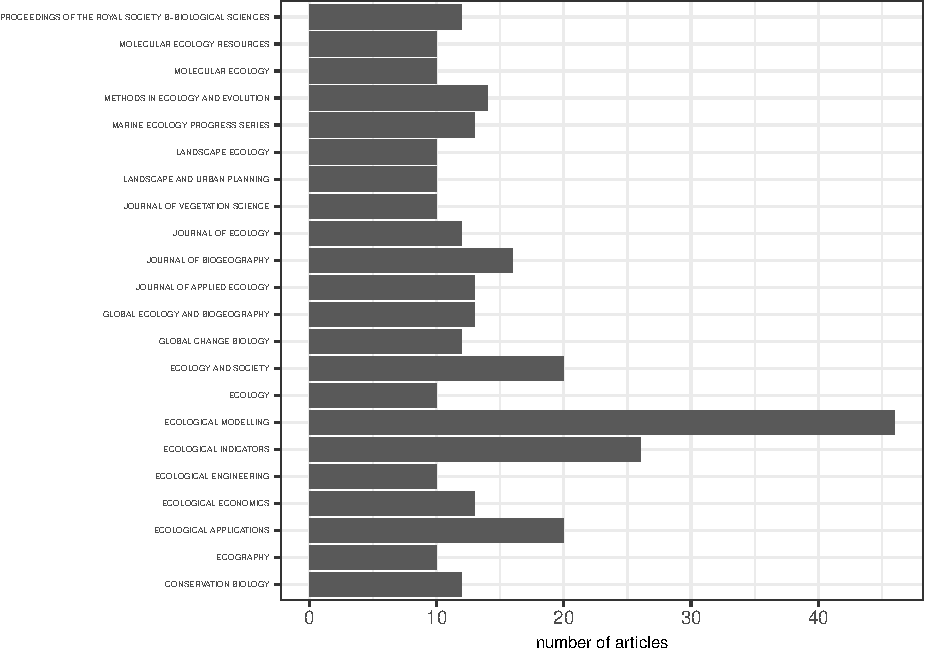
\includegraphics{_myDissertation_files/figure-latex/wosRegimePubsByJrnlmin10Pubs-1.pdf}
The search boolean for WoS boolean \emph{not} including restriction to fields (WC) `Ecology' and `Conservation Biology' yielded over 20,000 results. Restricting to the abovementioned fields created a manageable database from which to filter. This search yielded 2,776 articles. 654 of these papers included terms relating to `regime shifts' (Figure \ref{fig:wosRegimePubsByYear}), many appearing in the journal \emph{Ecological Modelling} (Figure \ref{fig:wosRegimePubsByJrnlmin10Pubs}). The rate of publication of `regime shift' articles is not strongly correlated with the rate of papers published in `Ecology' and `Biodiversity Conservation' fields (Figure \ref{fig:wosRegimePubsByYearwithNumEcolPubs}).
\begin{figure}
\centering
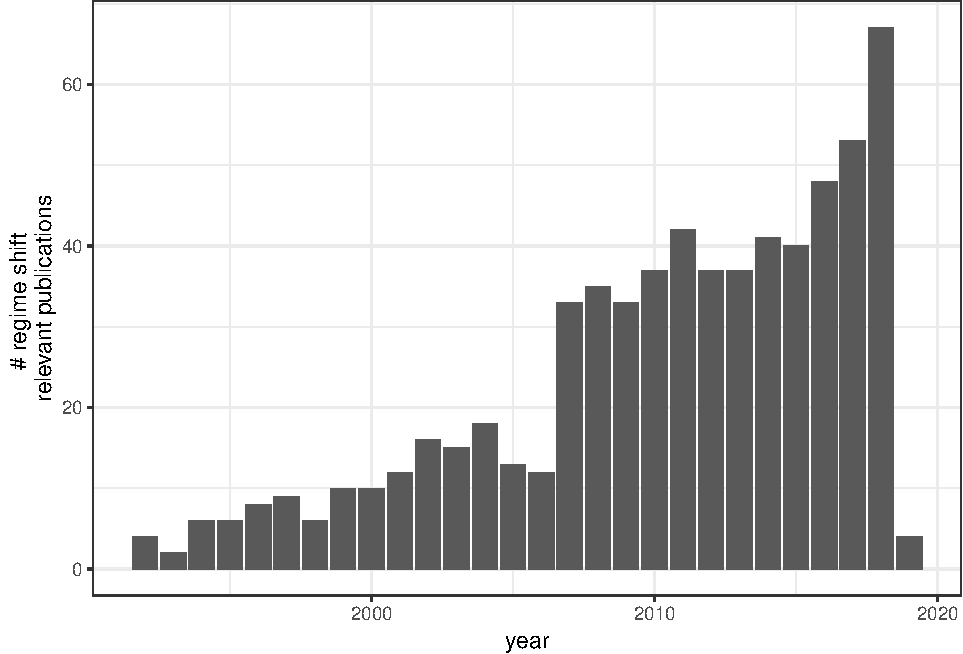
\includegraphics{_myDissertation_files/figure-latex/wosRegimePubsByYear-1.pdf}
\caption{\label{fig:wosRegimePubsByYear}Number of publications by year in fields `Ecology' and `Biodiversity Conservation' which included terms related to `regime shift' (total = 654).}
\end{figure}
Filtering the Web of Science results by including only articles mentioning terms related to `new method' yielded 202 articles. After removing prior knowledge, only 93 articles remained to be reviewed `by hand' (i.e., reading the entire paper). Of those reviewed I identified 2 `new' methods (\ref{fig:rdmReviewFlow}). Similarly, of the 250 articles reviewed from the Google Scholar search, I retained only 3 methods. I was previously aware of an additional 68 articles containing `new' methods (\ref{fig:rdmReviewFlow}), approximately half of which were identified using the abovementioned techniques.
\begin{figure}
\centering
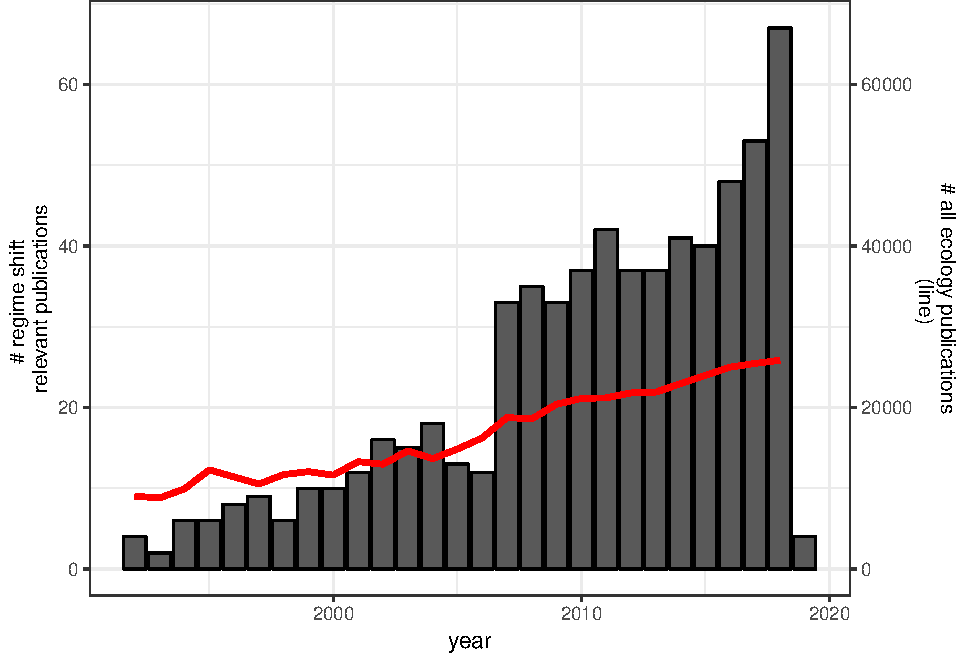
\includegraphics{_myDissertation_files/figure-latex/wosRegimePubsByYearwithNumEcolPubs-1.pdf}
\caption{\label{fig:wosRegimePubsByYearwithNumEcolPubs}Number of publications by year in fields `Ecology' and `Biodiversity Conservation' which included terms related to `regime shift' (total = 654).}
\end{figure}
\begin{figure}
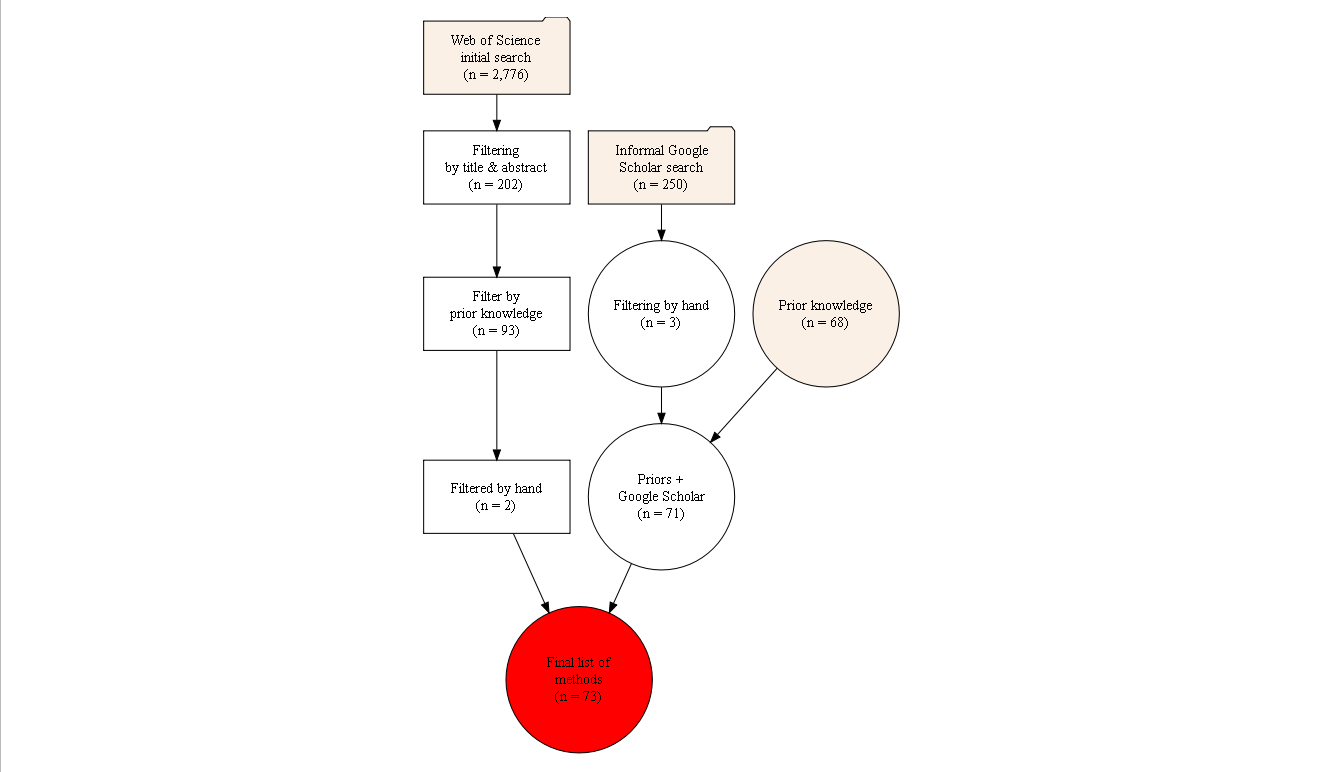
\includegraphics[width=0.95\linewidth]{./chapterFiles/rdmReview/figures/figsCalledInDiss/myDiagraph} \caption{Flowchart of the litearture review process for identifying new regime detection methods. *Only the first ten pages (250 articles) of Google Scholar results were examined. Node shapes: folder = unfiltered articles; box = articles actively filtered; diamond = number of articles with new methods.}\label{fig:rdmReviewFlow}
\end{figure}
\begin{verbatim}
Warning in pandoc.table.return(...): Supplied relative values don't add up
to 100%. Reverting to default
\end{verbatim}
\begin{longtable}[]{@{}lc@{}}
\caption{List of the regime detection methods identified in this review. (continued below)}\tabularnewline
\toprule
\begin{minipage}[b]{0.43\columnwidth}\raggedright
Method\strut
\end{minipage} & \begin{minipage}[b]{0.35\columnwidth}\centering
Metric type\strut
\end{minipage}\tabularnewline
\midrule
\endfirsthead
\toprule
\begin{minipage}[b]{0.43\columnwidth}\raggedright
Method\strut
\end{minipage} & \begin{minipage}[b]{0.35\columnwidth}\centering
Metric type\strut
\end{minipage}\tabularnewline
\midrule
\endhead
\begin{minipage}[t]{0.43\columnwidth}\raggedright
Characteristic length scale
(CLS) estimation\strut
\end{minipage} & \begin{minipage}[t]{0.35\columnwidth}\centering
attractor reconstruction\strut
\end{minipage}\tabularnewline
\begin{minipage}[t]{0.43\columnwidth}\raggedright
Average standard deviates\strut
\end{minipage} & \begin{minipage}[t]{0.35\columnwidth}\centering
metric\strut
\end{minipage}\tabularnewline
\begin{minipage}[t]{0.43\columnwidth}\raggedright
BDS test\strut
\end{minipage} & \begin{minipage}[t]{0.35\columnwidth}\centering
metric\strut
\end{minipage}\tabularnewline
\begin{minipage}[t]{0.43\columnwidth}\raggedright
Coefficient of variation (CV)\strut
\end{minipage} & \begin{minipage}[t]{0.35\columnwidth}\centering
metric\strut
\end{minipage}\tabularnewline
\begin{minipage}[t]{0.43\columnwidth}\raggedright
Conditional heteroskedasticity\strut
\end{minipage} & \begin{minipage}[t]{0.35\columnwidth}\centering
metric\strut
\end{minipage}\tabularnewline
\begin{minipage}[t]{0.43\columnwidth}\raggedright
Cumulative deviation test
(CUSUM)\strut
\end{minipage} & \begin{minipage}[t]{0.35\columnwidth}\centering
metric\strut
\end{minipage}\tabularnewline
\begin{minipage}[t]{0.43\columnwidth}\raggedright
Degenerate Fingerprinting\strut
\end{minipage} & \begin{minipage}[t]{0.35\columnwidth}\centering
metric\strut
\end{minipage}\tabularnewline
\begin{minipage}[t]{0.43\columnwidth}\raggedright
Degenerate Fingerprinting\strut
\end{minipage} & \begin{minipage}[t]{0.35\columnwidth}\centering
metric\strut
\end{minipage}\tabularnewline
\begin{minipage}[t]{0.43\columnwidth}\raggedright
Downton-Katz test\strut
\end{minipage} & \begin{minipage}[t]{0.35\columnwidth}\centering
metric\strut
\end{minipage}\tabularnewline
\begin{minipage}[t]{0.43\columnwidth}\raggedright
Fisher Information\strut
\end{minipage} & \begin{minipage}[t]{0.35\columnwidth}\centering
metric\strut
\end{minipage}\tabularnewline
\begin{minipage}[t]{0.43\columnwidth}\raggedright
Intervention Analysis\strut
\end{minipage} & \begin{minipage}[t]{0.35\columnwidth}\centering
metric\strut
\end{minipage}\tabularnewline
\begin{minipage}[t]{0.43\columnwidth}\raggedright
Inverse of AR(1) coefficient,
variance, etc.\strut
\end{minipage} & \begin{minipage}[t]{0.35\columnwidth}\centering
metric\strut
\end{minipage}\tabularnewline
\begin{minipage}[t]{0.43\columnwidth}\raggedright
Kurtosis\strut
\end{minipage} & \begin{minipage}[t]{0.35\columnwidth}\centering
metric\strut
\end{minipage}\tabularnewline
\begin{minipage}[t]{0.43\columnwidth}\raggedright
LePage test\strut
\end{minipage} & \begin{minipage}[t]{0.35\columnwidth}\centering
metric\strut
\end{minipage}\tabularnewline
\begin{minipage}[t]{0.43\columnwidth}\raggedright
Mann-Kendall test\strut
\end{minipage} & \begin{minipage}[t]{0.35\columnwidth}\centering
metric\strut
\end{minipage}\tabularnewline
\begin{minipage}[t]{0.43\columnwidth}\raggedright
Mann-whitney U-test\strut
\end{minipage} & \begin{minipage}[t]{0.35\columnwidth}\centering
metric\strut
\end{minipage}\tabularnewline
\begin{minipage}[t]{0.43\columnwidth}\raggedright
Moving detrended fluctuation
analysis (MDFA)\strut
\end{minipage} & \begin{minipage}[t]{0.35\columnwidth}\centering
metric\strut
\end{minipage}\tabularnewline
\begin{minipage}[t]{0.43\columnwidth}\raggedright
Nearest-neighbor statistics\strut
\end{minipage} & \begin{minipage}[t]{0.35\columnwidth}\centering
metric\strut
\end{minipage}\tabularnewline
\begin{minipage}[t]{0.43\columnwidth}\raggedright
Nikiforiv method\strut
\end{minipage} & \begin{minipage}[t]{0.35\columnwidth}\centering
metric\strut
\end{minipage}\tabularnewline
\begin{minipage}[t]{0.43\columnwidth}\raggedright
Oerleman's method\strut
\end{minipage} & \begin{minipage}[t]{0.35\columnwidth}\centering
metric\strut
\end{minipage}\tabularnewline
\begin{minipage}[t]{0.43\columnwidth}\raggedright
Pettitt test\strut
\end{minipage} & \begin{minipage}[t]{0.35\columnwidth}\centering
metric\strut
\end{minipage}\tabularnewline
\begin{minipage}[t]{0.43\columnwidth}\raggedright
Probability density function
entropy method\strut
\end{minipage} & \begin{minipage}[t]{0.35\columnwidth}\centering
metric\strut
\end{minipage}\tabularnewline
\begin{minipage}[t]{0.43\columnwidth}\raggedright
Quickest detection method
(ShiryaevRoberts
statistic)\strut
\end{minipage} & \begin{minipage}[t]{0.35\columnwidth}\centering
metric\strut
\end{minipage}\tabularnewline
\begin{minipage}[t]{0.43\columnwidth}\raggedright
Rodionov method\strut
\end{minipage} & \begin{minipage}[t]{0.35\columnwidth}\centering
metric\strut
\end{minipage}\tabularnewline
\begin{minipage}[t]{0.43\columnwidth}\raggedright
STARS\strut
\end{minipage} & \begin{minipage}[t]{0.35\columnwidth}\centering
metric\strut
\end{minipage}\tabularnewline
\begin{minipage}[t]{0.43\columnwidth}\raggedright
Sequential tests/moving
windows\strut
\end{minipage} & \begin{minipage}[t]{0.35\columnwidth}\centering
metric\strut
\end{minipage}\tabularnewline
\begin{minipage}[t]{0.43\columnwidth}\raggedright
Signal-to-noise ratio\strut
\end{minipage} & \begin{minipage}[t]{0.35\columnwidth}\centering
metric\strut
\end{minipage}\tabularnewline
\begin{minipage}[t]{0.43\columnwidth}\raggedright
Skewness\strut
\end{minipage} & \begin{minipage}[t]{0.35\columnwidth}\centering
metric\strut
\end{minipage}\tabularnewline
\begin{minipage}[t]{0.43\columnwidth}\raggedright
Spectral density ratio
indicator\strut
\end{minipage} & \begin{minipage}[t]{0.35\columnwidth}\centering
metric\strut
\end{minipage}\tabularnewline
\begin{minipage}[t]{0.43\columnwidth}\raggedright
Spectrum indicator\strut
\end{minipage} & \begin{minipage}[t]{0.35\columnwidth}\centering
metric\strut
\end{minipage}\tabularnewline
\begin{minipage}[t]{0.43\columnwidth}\raggedright
Stability Index of the
Ecological Units\strut
\end{minipage} & \begin{minipage}[t]{0.35\columnwidth}\centering
metric\strut
\end{minipage}\tabularnewline
\begin{minipage}[t]{0.43\columnwidth}\raggedright
Standard deviation (rising
variance)\strut
\end{minipage} & \begin{minipage}[t]{0.35\columnwidth}\centering
metric\strut
\end{minipage}\tabularnewline
\begin{minipage}[t]{0.43\columnwidth}\raggedright
Standard normal homoegeneity\strut
\end{minipage} & \begin{minipage}[t]{0.35\columnwidth}\centering
metric\strut
\end{minipage}\tabularnewline
\begin{minipage}[t]{0.43\columnwidth}\raggedright
T-test\strut
\end{minipage} & \begin{minipage}[t]{0.35\columnwidth}\centering
metric\strut
\end{minipage}\tabularnewline
\begin{minipage}[t]{0.43\columnwidth}\raggedright
Threshold Indicator Taxa
ANalysis (TITAN)\strut
\end{minipage} & \begin{minipage}[t]{0.35\columnwidth}\centering
metric\strut
\end{minipage}\tabularnewline
\begin{minipage}[t]{0.43\columnwidth}\raggedright
Variance Index\strut
\end{minipage} & \begin{minipage}[t]{0.35\columnwidth}\centering
metric\strut
\end{minipage}\tabularnewline
\begin{minipage}[t]{0.43\columnwidth}\raggedright
Wilcoxon rank-sum\strut
\end{minipage} & \begin{minipage}[t]{0.35\columnwidth}\centering
metric\strut
\end{minipage}\tabularnewline
\begin{minipage}[t]{0.43\columnwidth}\raggedright
dimension reduction techniques
(e.g., PCA)\strut
\end{minipage} & \begin{minipage}[t]{0.35\columnwidth}\centering
metric\strut
\end{minipage}\tabularnewline
\begin{minipage}[t]{0.43\columnwidth}\raggedright
NA\strut
\end{minipage} & \begin{minipage}[t]{0.35\columnwidth}\centering
metric\strut
\end{minipage}\tabularnewline
\begin{minipage}[t]{0.43\columnwidth}\raggedright
NA\strut
\end{minipage} & \begin{minipage}[t]{0.35\columnwidth}\centering
metric\strut
\end{minipage}\tabularnewline
\begin{minipage}[t]{0.43\columnwidth}\raggedright
NA\strut
\end{minipage} & \begin{minipage}[t]{0.35\columnwidth}\centering
metric\strut
\end{minipage}\tabularnewline
\begin{minipage}[t]{0.43\columnwidth}\raggedright
two-phase regression\strut
\end{minipage} & \begin{minipage}[t]{0.35\columnwidth}\centering
metric of a model\strut
\end{minipage}\tabularnewline
\begin{minipage}[t]{0.43\columnwidth}\raggedright
Zonal thresholding\strut
\end{minipage} & \begin{minipage}[t]{0.35\columnwidth}\centering
metric*\strut
\end{minipage}\tabularnewline
\begin{minipage}[t]{0.43\columnwidth}\raggedright
Bayesian approaches\strut
\end{minipage} & \begin{minipage}[t]{0.35\columnwidth}\centering
model\strut
\end{minipage}\tabularnewline
\begin{minipage}[t]{0.43\columnwidth}\raggedright
Convex model\strut
\end{minipage} & \begin{minipage}[t]{0.35\columnwidth}\centering
model\strut
\end{minipage}\tabularnewline
\begin{minipage}[t]{0.43\columnwidth}\raggedright
Generalized model\strut
\end{minipage} & \begin{minipage}[t]{0.35\columnwidth}\centering
model\strut
\end{minipage}\tabularnewline
\begin{minipage}[t]{0.43\columnwidth}\raggedright
Multivariable autoregressive
models (MAR1)\strut
\end{minipage} & \begin{minipage}[t]{0.35\columnwidth}\centering
model\strut
\end{minipage}\tabularnewline
\begin{minipage}[t]{0.43\columnwidth}\raggedright
Nonparametric
drift-diffusion-jump model\strut
\end{minipage} & \begin{minipage}[t]{0.35\columnwidth}\centering
model\strut
\end{minipage}\tabularnewline
\begin{minipage}[t]{0.43\columnwidth}\raggedright
Potential analysis\strut
\end{minipage} & \begin{minipage}[t]{0.35\columnwidth}\centering
model\strut
\end{minipage}\tabularnewline
\begin{minipage}[t]{0.43\columnwidth}\raggedright
Regression-based models\strut
\end{minipage} & \begin{minipage}[t]{0.35\columnwidth}\centering
model\strut
\end{minipage}\tabularnewline
\begin{minipage}[t]{0.43\columnwidth}\raggedright
Self-exciting threshold
autoregressive state-space
model SETARSS(p)\strut
\end{minipage} & \begin{minipage}[t]{0.35\columnwidth}\centering
model\strut
\end{minipage}\tabularnewline
\begin{minipage}[t]{0.43\columnwidth}\raggedright
Smooth transition
autoregressive model\strut
\end{minipage} & \begin{minipage}[t]{0.35\columnwidth}\centering
model\strut
\end{minipage}\tabularnewline
\begin{minipage}[t]{0.43\columnwidth}\raggedright
shiftogram\strut
\end{minipage} & \begin{minipage}[t]{0.35\columnwidth}\centering
model\strut
\end{minipage}\tabularnewline
\begin{minipage}[t]{0.43\columnwidth}\raggedright
Autocorrelation at-lag-1\strut
\end{minipage} & \begin{minipage}[t]{0.35\columnwidth}\centering
model-based\strut
\end{minipage}\tabularnewline
\begin{minipage}[t]{0.43\columnwidth}\raggedright
Online dynamic linear
modelling + time\_varying
autoregressive state\_space
models (TVARSS)\strut
\end{minipage} & \begin{minipage}[t]{0.35\columnwidth}\centering
models\strut
\end{minipage}\tabularnewline
\begin{minipage}[t]{0.43\columnwidth}\raggedright
Clustering, various\strut
\end{minipage} & \begin{minipage}[t]{0.35\columnwidth}\centering
NA\strut
\end{minipage}\tabularnewline
\begin{minipage}[t]{0.43\columnwidth}\raggedright
Degenerate Fingerprinting\strut
\end{minipage} & \begin{minipage}[t]{0.35\columnwidth}\centering
NA\strut
\end{minipage}\tabularnewline
\begin{minipage}[t]{0.43\columnwidth}\raggedright
Fourier Analysis\strut
\end{minipage} & \begin{minipage}[t]{0.35\columnwidth}\centering
NA\strut
\end{minipage}\tabularnewline
\begin{minipage}[t]{0.43\columnwidth}\raggedright
Free-knot splines \& piecewise
linear modelling\strut
\end{minipage} & \begin{minipage}[t]{0.35\columnwidth}\centering
NA\strut
\end{minipage}\tabularnewline
\begin{minipage}[t]{0.43\columnwidth}\raggedright
Lanzante method\strut
\end{minipage} & \begin{minipage}[t]{0.35\columnwidth}\centering
NA\strut
\end{minipage}\tabularnewline
\begin{minipage}[t]{0.43\columnwidth}\raggedright
MCMC\strut
\end{minipage} & \begin{minipage}[t]{0.35\columnwidth}\centering
NA\strut
\end{minipage}\tabularnewline
\begin{minipage}[t]{0.43\columnwidth}\raggedright
Method 1-TBD\strut
\end{minipage} & \begin{minipage}[t]{0.35\columnwidth}\centering
NA\strut
\end{minipage}\tabularnewline
\begin{minipage}[t]{0.43\columnwidth}\raggedright
Method 2-TBD\strut
\end{minipage} & \begin{minipage}[t]{0.35\columnwidth}\centering
NA\strut
\end{minipage}\tabularnewline
\begin{minipage}[t]{0.43\columnwidth}\raggedright
Vector-autoregressive method\strut
\end{minipage} & \begin{minipage}[t]{0.35\columnwidth}\centering
NA\strut
\end{minipage}\tabularnewline
\begin{minipage}[t]{0.43\columnwidth}\raggedright
Wavelet analysis
(decomposition)\strut
\end{minipage} & \begin{minipage}[t]{0.35\columnwidth}\centering
NA\strut
\end{minipage}\tabularnewline
\begin{minipage}[t]{0.43\columnwidth}\raggedright
method-fuzzy synthetic
evaluation (FSE)\strut
\end{minipage} & \begin{minipage}[t]{0.35\columnwidth}\centering
NA\strut
\end{minipage}\tabularnewline
\bottomrule
\end{longtable}
\begin{longtable}[]{@{}c@{}}
\toprule
\begin{minipage}[b]{0.46\columnwidth}\centering
Source\strut
\end{minipage}\tabularnewline
\midrule
\endhead
\begin{minipage}[t]{0.46\columnwidth}\centering
@NA\strut
\end{minipage}\tabularnewline
\begin{minipage}[t]{0.46\columnwidth}\centering
@ebbesmeyer19911976\strut
\end{minipage}\tabularnewline
\begin{minipage}[t]{0.46\columnwidth}\centering
@carpenterBrock2011early\strut
\end{minipage}\tabularnewline
\begin{minipage}[t]{0.46\columnwidth}\centering
@NA\strut
\end{minipage}\tabularnewline
\begin{minipage}[t]{0.46\columnwidth}\centering
@seekell2011conditional\strut
\end{minipage}\tabularnewline
\begin{minipage}[t]{0.46\columnwidth}\centering
@buishand1982some\strut
\end{minipage}\tabularnewline
\begin{minipage}[t]{0.46\columnwidth}\centering
@held2004detection\strut
\end{minipage}\tabularnewline
\begin{minipage}[t]{0.46\columnwidth}\centering
@livina2007modified\strut
\end{minipage}\tabularnewline
\begin{minipage}[t]{0.46\columnwidth}\centering
@karl1987approach\strut
\end{minipage}\tabularnewline
\begin{minipage}[t]{0.46\columnwidth}\centering
@fath\_regime\_2003\strut
\end{minipage}\tabularnewline
\begin{minipage}[t]{0.46\columnwidth}\centering
@francis1994decadal\strut
\end{minipage}\tabularnewline
\begin{minipage}[t]{0.46\columnwidth}\centering
@carpenter2008leading\strut
\end{minipage}\tabularnewline
\begin{minipage}[t]{0.46\columnwidth}\centering
@biggs2009turning\strut
\end{minipage}\tabularnewline
\begin{minipage}[t]{0.46\columnwidth}\centering
@yonetani1993detection\strut
\end{minipage}\tabularnewline
\begin{minipage}[t]{0.46\columnwidth}\centering
@goossens1987recognize\strut
\end{minipage}\tabularnewline
\begin{minipage}[t]{0.46\columnwidth}\centering
@mauget2003multidecadal\strut
\end{minipage}\tabularnewline
\begin{minipage}[t]{0.46\columnwidth}\centering
@he2008new\strut
\end{minipage}\tabularnewline
\begin{minipage}[t]{0.46\columnwidth}\centering
@pawlowski\_identification\_2008\strut
\end{minipage}\tabularnewline
\begin{minipage}[t]{0.46\columnwidth}\centering
@NA\strut
\end{minipage}\tabularnewline
\begin{minipage}[t]{0.46\columnwidth}\centering
@oerlemans1978objective\strut
\end{minipage}\tabularnewline
\begin{minipage}[t]{0.46\columnwidth}\centering
@pettitt1979non\strut
\end{minipage}\tabularnewline
\begin{minipage}[t]{0.46\columnwidth}\centering
@pawlowski\_identification\_2008\strut
\end{minipage}\tabularnewline
\begin{minipage}[t]{0.46\columnwidth}\centering
@moustakides2009numerical\strut
\end{minipage}\tabularnewline
\begin{minipage}[t]{0.46\columnwidth}\centering
@rodionov\_sequential\_2005\strut
\end{minipage}\tabularnewline
\begin{minipage}[t]{0.46\columnwidth}\centering
@buishand1982some\strut
\end{minipage}\tabularnewline
\begin{minipage}[t]{0.46\columnwidth}\centering
@NA\strut
\end{minipage}\tabularnewline
\begin{minipage}[t]{0.46\columnwidth}\centering
@NA\strut
\end{minipage}\tabularnewline
\begin{minipage}[t]{0.46\columnwidth}\centering
@guttal2008changing\strut
\end{minipage}\tabularnewline
\begin{minipage}[t]{0.46\columnwidth}\centering
@biggs2009turning\strut
\end{minipage}\tabularnewline
\begin{minipage}[t]{0.46\columnwidth}\centering
@NA\strut
\end{minipage}\tabularnewline
\begin{minipage}[t]{0.46\columnwidth}\centering
@parparov2015quantifying\strut
\end{minipage}\tabularnewline
\begin{minipage}[t]{0.46\columnwidth}\centering
@carpenter2006rising\strut
\end{minipage}\tabularnewline
\begin{minipage}[t]{0.46\columnwidth}\centering
@alexandersson1986homogeneity\strut
\end{minipage}\tabularnewline
\begin{minipage}[t]{0.46\columnwidth}\centering
@ducre2003comparison\strut
\end{minipage}\tabularnewline
\begin{minipage}[t]{0.46\columnwidth}\centering
@baker2010new\strut
\end{minipage}\tabularnewline
\begin{minipage}[t]{0.46\columnwidth}\centering
@brock\_variance\_2006\strut
\end{minipage}\tabularnewline
\begin{minipage}[t]{0.46\columnwidth}\centering
@karl1987approach\strut
\end{minipage}\tabularnewline
\begin{minipage}[t]{0.46\columnwidth}\centering
@NA\strut
\end{minipage}\tabularnewline
\begin{minipage}[t]{0.46\columnwidth}\centering
@ives2003estimating\strut
\end{minipage}\tabularnewline
\begin{minipage}[t]{0.46\columnwidth}\centering
@NA\strut
\end{minipage}\tabularnewline
\begin{minipage}[t]{0.46\columnwidth}\centering
@andersen\_ecological\_2009,\strut
\end{minipage}\tabularnewline
\begin{minipage}[t]{0.46\columnwidth}\centering
@easterling1995new\strut
\end{minipage}\tabularnewline
\begin{minipage}[t]{0.46\columnwidth}\centering
@yin2017methods\strut
\end{minipage}\tabularnewline
\begin{minipage}[t]{0.46\columnwidth}\centering
@jo2016bayesian\strut
\end{minipage}\tabularnewline
\begin{minipage}[t]{0.46\columnwidth}\centering
@qi2016resilience\strut
\end{minipage}\tabularnewline
\begin{minipage}[t]{0.46\columnwidth}\centering
@lade2012early\strut
\end{minipage}\tabularnewline
\begin{minipage}[t]{0.46\columnwidth}\centering
@ives2012detecting\strut
\end{minipage}\tabularnewline
\begin{minipage}[t]{0.46\columnwidth}\centering
@carpenter2011early\strut
\end{minipage}\tabularnewline
\begin{minipage}[t]{0.46\columnwidth}\centering
@ives2012detecting\strut
\end{minipage}\tabularnewline
\begin{minipage}[t]{0.46\columnwidth}\centering
@solow1987testing\strut
\end{minipage}\tabularnewline
\begin{minipage}[t]{0.46\columnwidth}\centering
@tong1990nonlinear\strut
\end{minipage}\tabularnewline
\begin{minipage}[t]{0.46\columnwidth}\centering
@see gal2010novel\strut
\end{minipage}\tabularnewline
\begin{minipage}[t]{0.46\columnwidth}\centering
@groger2011analyses\strut
\end{minipage}\tabularnewline
\begin{minipage}[t]{0.46\columnwidth}\centering
@vincent1998technique\strut
\end{minipage}\tabularnewline
\begin{minipage}[t]{0.46\columnwidth}\centering
@parparov2017quantifying\strut
\end{minipage}\tabularnewline
\begin{minipage}[t]{0.46\columnwidth}\centering
@NA\strut
\end{minipage}\tabularnewline
\begin{minipage}[t]{0.46\columnwidth}\centering
@kleinen2003potential\strut
\end{minipage}\tabularnewline
\begin{minipage}[t]{0.46\columnwidth}\centering
@carpenter2010early\strut
\end{minipage}\tabularnewline
\begin{minipage}[t]{0.46\columnwidth}\centering
@gal2010novel\strut
\end{minipage}\tabularnewline
\begin{minipage}[t]{0.46\columnwidth}\centering
@lanzante1996resistant\strut
\end{minipage}\tabularnewline
\begin{minipage}[t]{0.46\columnwidth}\centering
@NA\strut
\end{minipage}\tabularnewline
\begin{minipage}[t]{0.46\columnwidth}\centering
@manly2006two\strut
\end{minipage}\tabularnewline
\begin{minipage}[t]{0.46\columnwidth}\centering
@manly2006two\strut
\end{minipage}\tabularnewline
\begin{minipage}[t]{0.46\columnwidth}\centering
@solow\_test\_2005\strut
\end{minipage}\tabularnewline
\begin{minipage}[t]{0.46\columnwidth}\centering
@cazelles2008wavelet\strut
\end{minipage}\tabularnewline
\begin{minipage}[t]{0.46\columnwidth}\centering
@wang2011application\strut
\end{minipage}\tabularnewline
\bottomrule
\end{longtable}
Using my prior knowledge of the relevant literature and by systematically searching the Web of Science and Google Scholar databases, I identified 66 unique regime detection measures (Figure \ref{fig:rdmReviewFlow}; Table \ref{tab:methodsMetricsListTab1}).
\begin{figure}
\centering
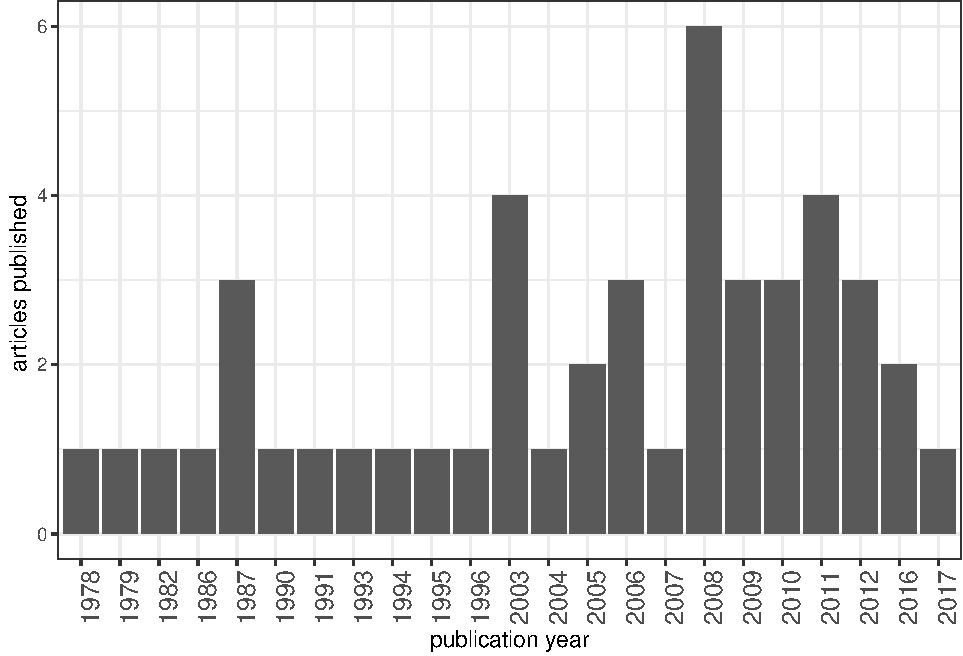
\includegraphics{_myDissertation_files/figure-latex/jrnlYearFig-1.pdf}
\caption{\label{fig:jrnlYearFig}Number of methods published over time.}
\end{figure}
\hypertarget{bibliographic-analysis-of-ecological-regime-shift-literature-1}{%
\subsection{2. Bibliographic analysis of ecological regime shift literature}\label{bibliographic-analysis-of-ecological-regime-shift-literature-1}}

A search of Web of Science for articles in Ecology and Biodiversity Conservation containing phrases related to `regime shifts' yielded 1,636 original articles. These articles were not filtered in any fashion and as such all were considered in the bibliographic analysis.

I used the clustering algorithms of the bibliometrics package to produce a thematic map which uses a clustering algorithm to identify clusters (or themes) based on keywords associated with each article (Cobo, López-Herrera, Herrera-Viedma, \& Herrera, 2011). Keywords are supplied both by the authors and by the ISI Web of Science and appear to be used very differently among this literature (Figure @ref(fig:thematicMaps\_keyword)). The clustering algorithm identified fewer clusters (themes) in the ISI-keywords (Figure @ref(fig:thematicMaps\_keyword)a) than were identified among the author-supplied keywords (Figure @ref(fig:thematicMaps\_keyword)b). This pattern is not surprising given the former keywords are restricted to pre-set themes while the authors can often supply any words. The themes identified in the ISI-keyword analysis were relatively consistent as the number of keywords analysed increasded (Figure @ref(fig:thematicMaps\_keyword\_isi)), but the themes varied drastically among the author-supplied keywords (Figure @ref(fig:thematicMaps\_keyword\_author)). For this reason I make inference on only the ISI-supplied keyword cluster analysis.

Four major themes were identified in the ISI keyword analysis and, interestingly, mostly fell within the two extreme quadrants, the first and the third (Figure @ref(fig:thematicMaps\_keyword\_isi)). The themes identified by ISI keywords were much larger in scope (e.g, dymamics, ecosystems, climate; (Figure @ref(fig:thematicMaps\_keyword)a) than those identified in the author keywords (e.g., eutrophication, trophic cascade; Figure @ref(fig:thematicMaps\_keyword)b). Regime shifts and ecosystems dynamics are usually have both high centrality and density (Figure @ref(fig:thematicMaps\_keyword)b:d), suggesting these two themes are both important to the development of the field and still strongly influence the field. Although dynamics (i.e.~non-linearity) plays a central role in the theory of ecological systems this is not reflected in many case studies of regime shifts in application (Litzow \& Hunsicker, 2016). Litzow \& Hunsicker (2016) found that \(\sim50%
\) of case studies using early warning indicators to identify regime shifts in time series actually tested and/or accounted for non-linear dymamics in the data.

A few patterns appear in analyses of the intellectual structure of regime shift research in ecology (Figure \ref{fig:historiograph}). First, although the concept of stability, thresholds, and multiple stable states in ecological systems first appeared (and was well-receieved) in the literature in the 1970s {[}e.g., Holling (1973);@ may1977thresholds{]}, the most important papers in this field appeared primarily in the early and mid 2000s (Scheffer \& Carpenter, 2003; @ carpenter2006rising;@ folke2004regime; Walker, Holling, Carpenter, \& Kinzig, 2004; Nes \& Scheffer, 2005). The most recent major contributions to the field were concpetual works emphasizing planetery boundaries and tiping points and the impacts of not recognizing these shifts (Hughes, Carpenter, Rockström, Scheffer, \& Walker, 2013). Finally, the ``rise'' of resilience theory (Folke et al., 2004; Walker et al., 2004), the first efforts of a search for early warning indicators of ecological regime shifts (Carpenter \& Brock, 2006) and a spur of critique of regime shift detection methods {[}Andersen et al. (2009);@ contamin\_indicators\_2009{]} are recognized in the historiograph.

The clustering algorithm identified the most influential papers in the field (based solely on number of citations) as those published in the late 2000s (Fig \ref{fig:totArtCitesPerYear}), articles which are broad in-scope and are still used today to frame studies in the context of global change, planetary boundaries, and large-scale tipping points (Bennett, Peterson, \& Gordon, 2009; Rockstr??m et al., 2009; Smith \& Schindler, 2009). Arguably, the papers that are equally influential include those which correspond with the observed rapid increase in the number of publications (in the early 2000s), Folke et al. (2004) and Scheffer \& Carpenter (2003) (Fig \ref{fig:totArtCitesPerYear}).
\begin{Shaded}
\begin{Highlighting}[]
\NormalTok{knitr}\OperatorTok{::}\KeywordTok{include_graphics}\NormalTok{(here}\OperatorTok{::}\KeywordTok{here}\NormalTok{(}\StringTok{"chapterFiles/rdmReview/figures/figsCalledInDiss/historiograph_75quantile.png"}\NormalTok{))}
\end{Highlighting}
\end{Shaded}
\begin{figure}
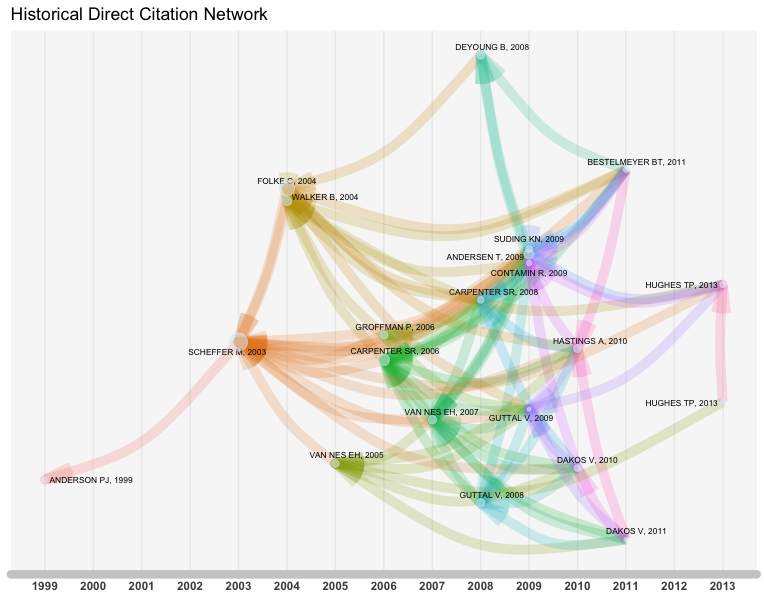
\includegraphics[width=0.85\linewidth]{/Users/jessicaburnett/Documents/GitHub/myDissertation/chapterFiles/rdmReview/figures/figsCalledInDiss/historiograph_75quantile} \caption{Chronological direct citation newtwork suggests the intellectual structure can be mapped to a few papers. This historiograph identifies important works explicitly in chronological, as opposed to absolute, order.}\label{fig:historiograph}
\end{figure}
\begin{Shaded}
\begin{Highlighting}[]
\NormalTok{knitr}\OperatorTok{::}\KeywordTok{include_graphics}\NormalTok{(here}\OperatorTok{::}\KeywordTok{here}\NormalTok{(}\StringTok{"chapterFiles/rdmReview/figures/figsCalledInDiss/totArtCitesPerYear.png"}\NormalTok{))}
\end{Highlighting}
\end{Shaded}
\begin{figure}
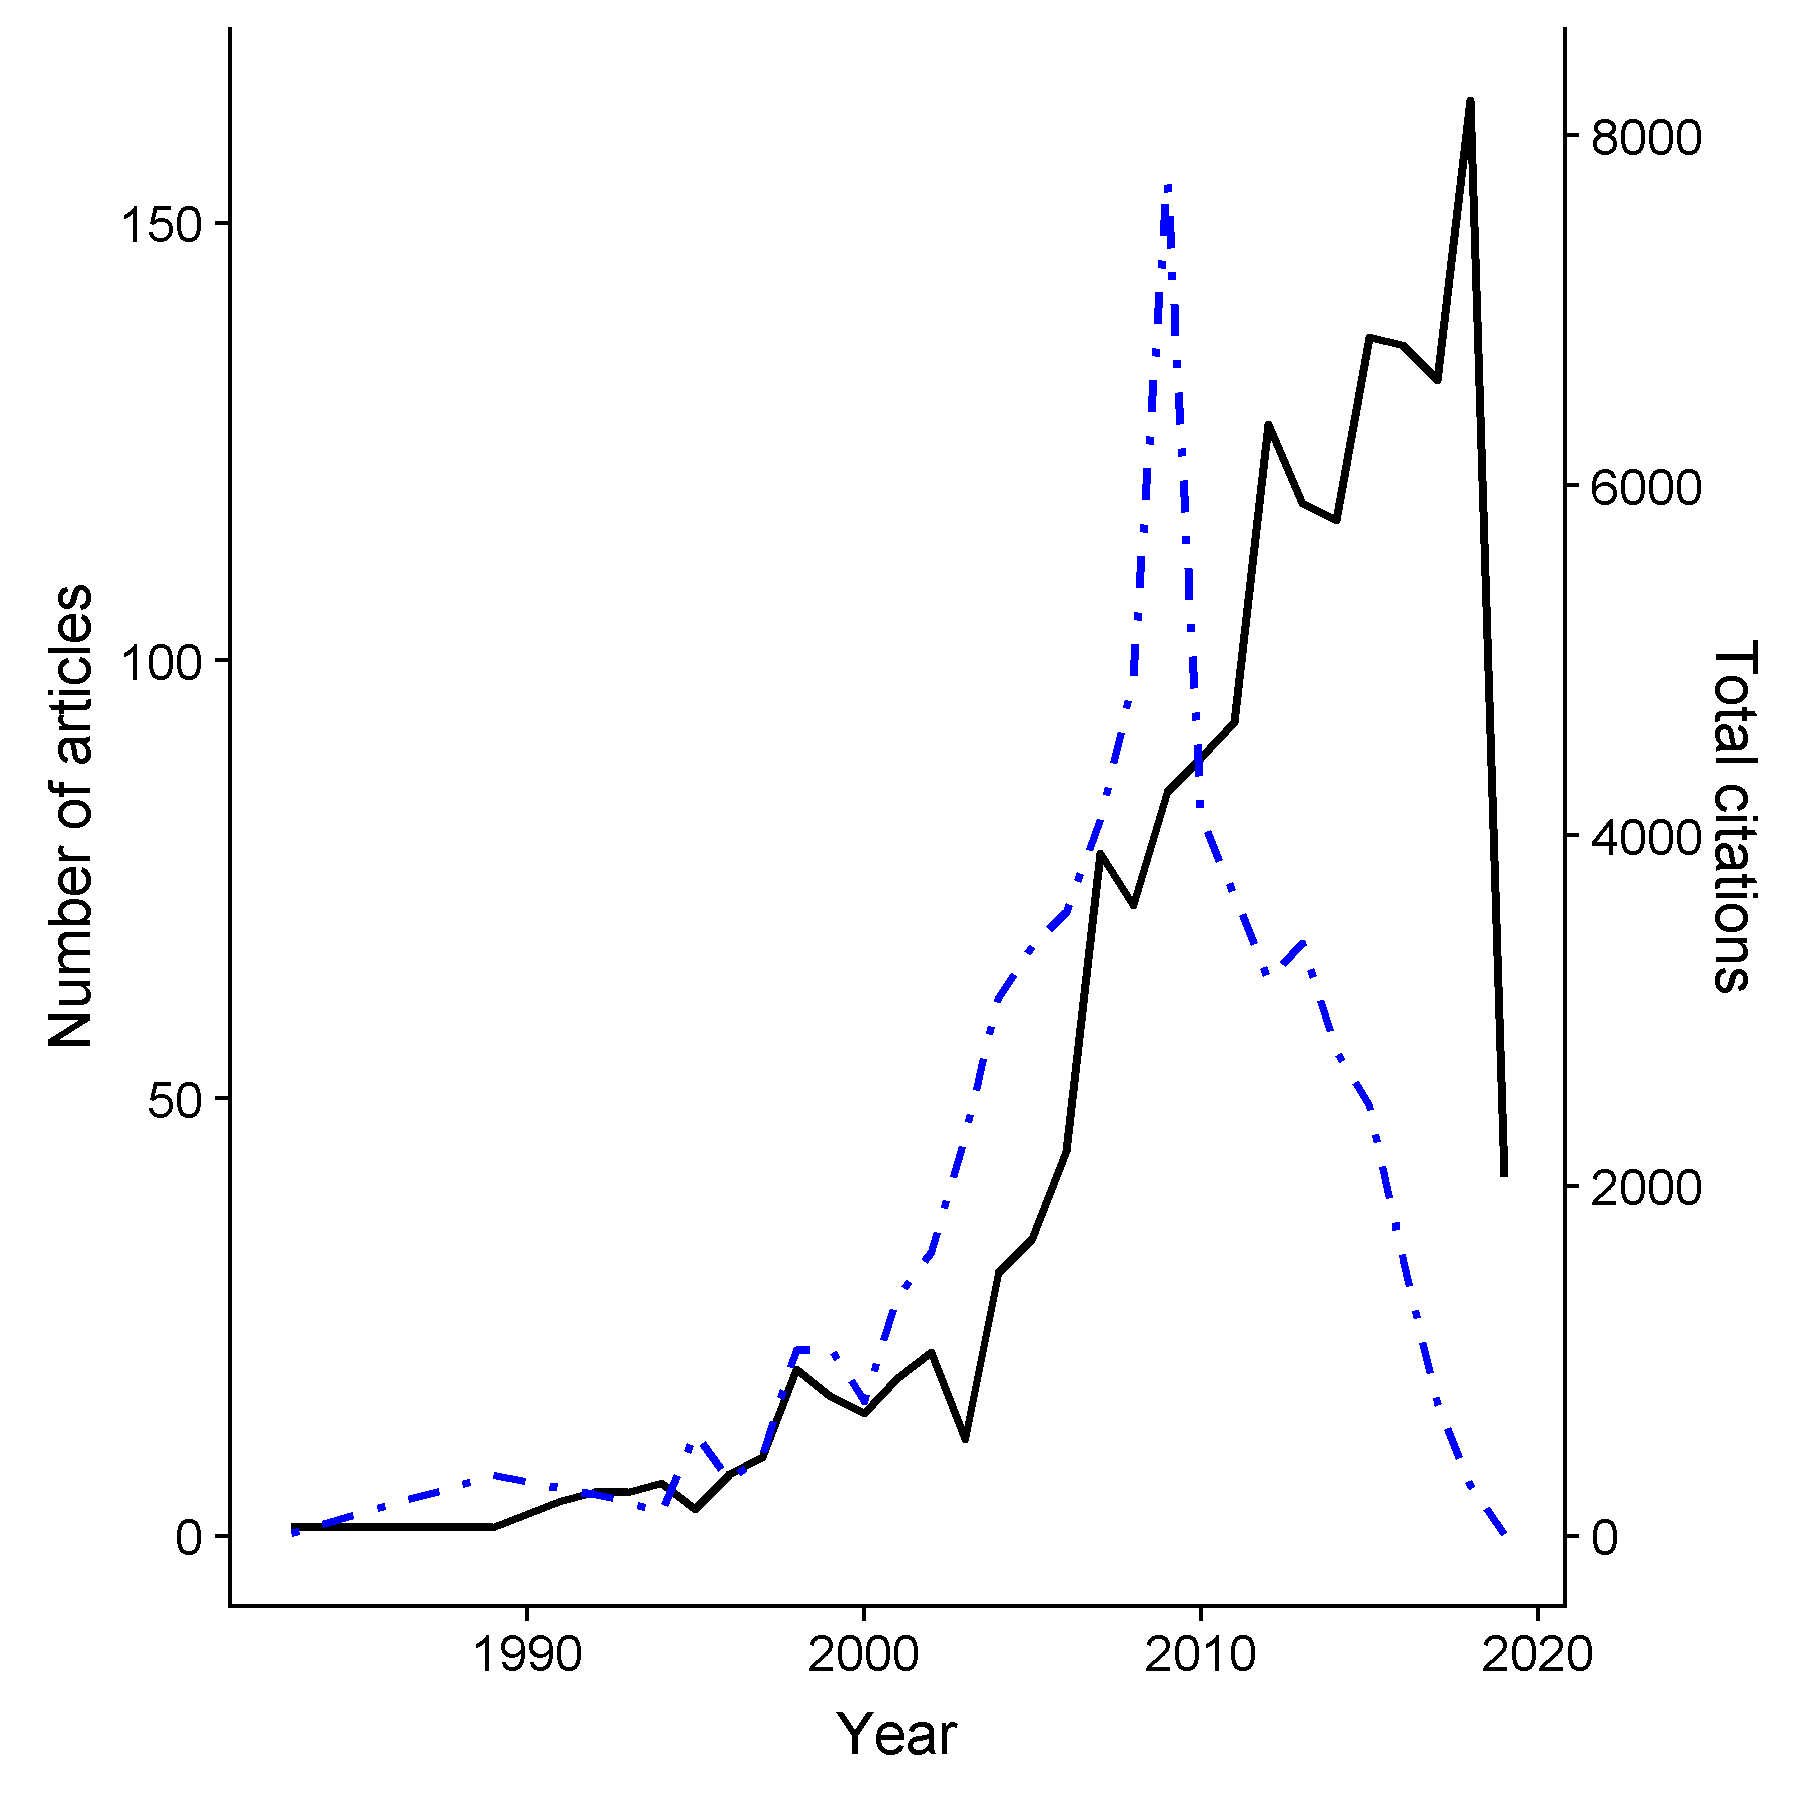
\includegraphics[width=0.85\linewidth]{/Users/jessicaburnett/Documents/GitHub/myDissertation/chapterFiles/rdmReview/figures/figsCalledInDiss/totArtCitesPerYear} \caption{Total number of articles published and corresponding number of citations (for papers published that year). The most highly cited papers to-date are those published in the late 2000s.}\label{fig:totArtCitesPerYear}
\end{figure}
\begin{Shaded}
\begin{Highlighting}[]
\NormalTok{knitr}\OperatorTok{::}\KeywordTok{include_graphics}\NormalTok{(here}\OperatorTok{::}\KeywordTok{here}\NormalTok{(}\StringTok{"chapterFiles/rdmReview/figures/figsCalledInDiss/revArtNums.png"}\NormalTok{))}
\end{Highlighting}
\end{Shaded}
\begin{figure}
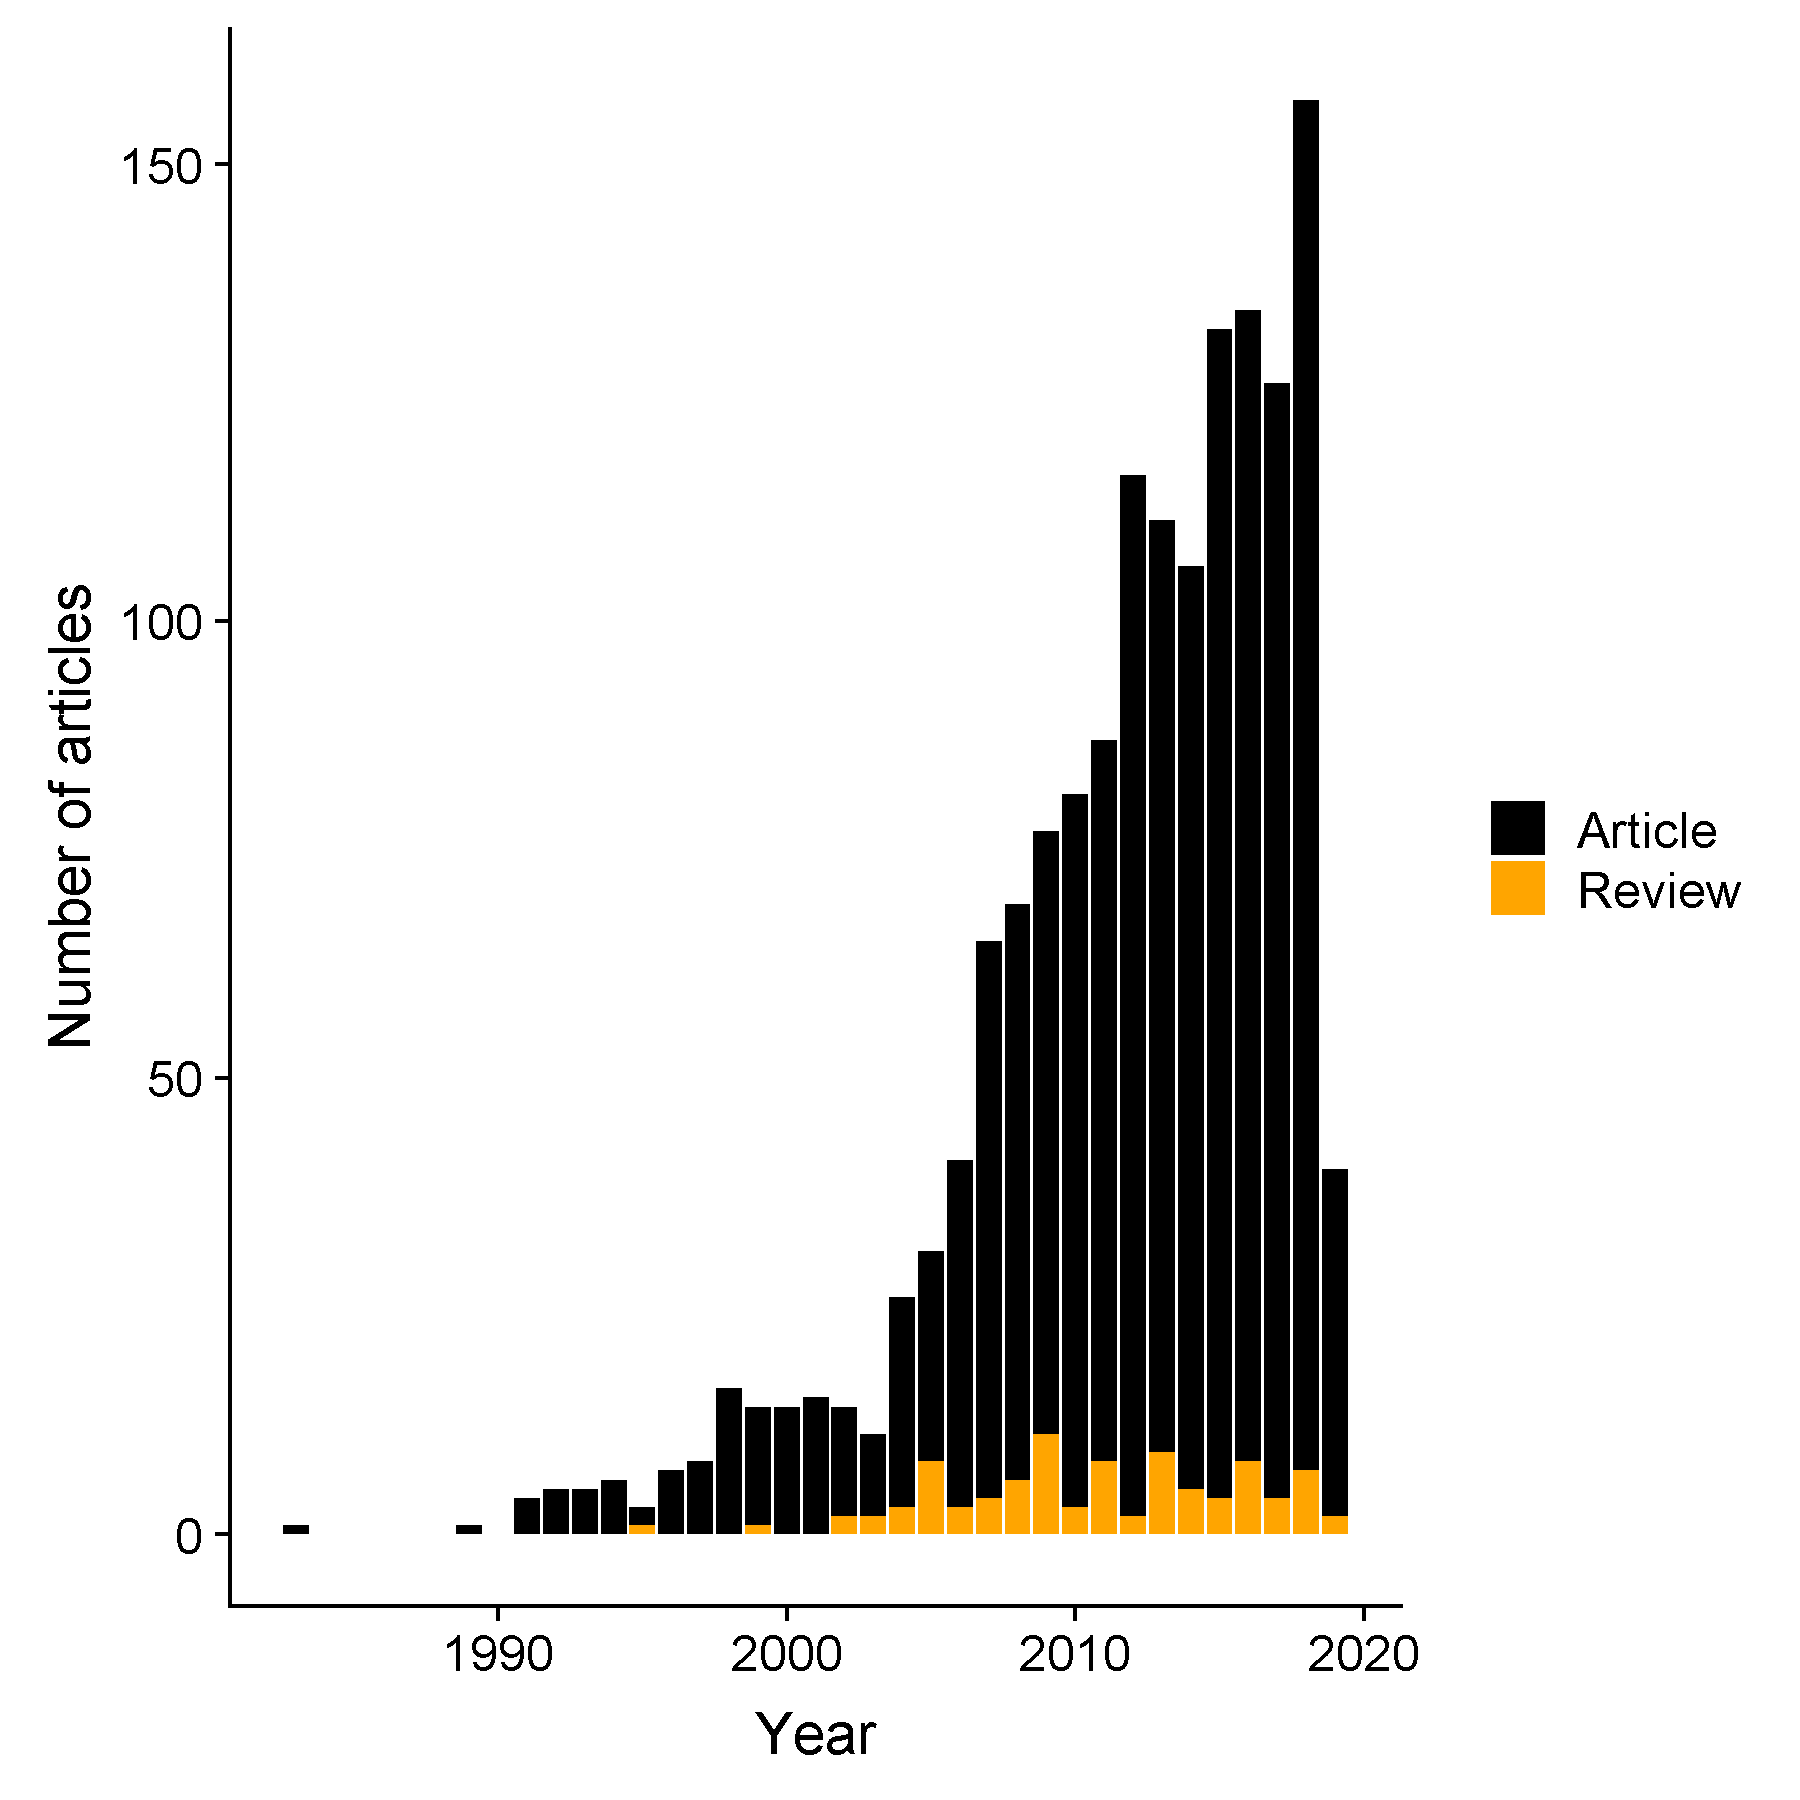
\includegraphics[width=0.85\linewidth]{/Users/jessicaburnett/Documents/GitHub/myDissertation/chapterFiles/rdmReview/figures/figsCalledInDiss/revArtNums} \caption{Total number of articles published per year by category as categorized by ISI. Book chapters, proceedings, editorials, and letters are excluded.}\label{fig:revArtNums}
\end{figure}
Numerous reviews of the regime shift literature exist, ranging from conceptual reviews of the state of regime shift theory in ecology and application {[}e.g., Bestelmeyer et al. (2011);@ mac2014scrutiny;@ andersen\_ecological\_2009{]}, to studies of robustness of early warning indicators under various theoretical and practical conditions {[}e.g., Dutta, Sharma, \& Abbott (2018); Perretti \& Munch (2012); Lindegren et al. (2012); Hastings \& Wysham (2010a); Figure \ref{fig:revArtNums}{]}. Further, comprehensive reviews of the ecological regime shift detetion literautre are increasingly out-dated. A permanent and open-source database containing information critical to the testing, comparison, and implementation of RDMs may prove useful to the reader who is interested in applying RDMs but is lacking the statistical or mathematical background to do so.

The early warning indicators that are often referred to as, ``traditional early warning indicators'' (variance, skewness, autocorrelation at lag-1) are fairly well-reviewed, and have been tested under a variety of conditions (Dakos, Carpenter, et al., 2012; @ ditlevsen2010tipping; Lindegren et al., 2012; Boettiger \& Hastings, 2012; Dutta et al., 2018; Litzow \& Hunsicker, 2016; Perretti \& Munch, 2012; Sommer, Benthem, Fontaneto, \& Ozgul, 2017). However, many of these works apply the traditional (and other) early warning indicators to simulated data, with only some (Contamin \& Ellison, 2009; Dutta et al., 2018; Guttal, Jayaprakash, \& Tabbaa, 2013; Perretti \& Munch, 2012) testing under varying conditions of noise and expected shift types. The utility and robustness of the traditional early warning indicators is not consistent across and within sytems, making them of limited utility in situations where the system cannot be reliably mathematically modelled, or where we have limited data {[}see also Ch. \ref{resampling}{]}. The authors of most reviews and comparative studies of early warning indicators suggest that no early warning indicator is reliable alone, or that work is needed to understand under what empirical conditions early warning indicators might fail (Clements \& Ozgul, 2018; deYoung et al., 2008; Filatova et al., 2016; Kefi et al., 2014).

\hypertarget{a-synthesis-of-the-methods-available-for-the-practical-ecologist}{%
\section{A synthesis of the methods available for the practical ecologist}\label{a-synthesis-of-the-methods-available-for-the-practical-ecologist}}

Many of the methods identified in this review have yet to be tested on multiple, empirical data (see Table \ref{tab:methodsMetricsListTab1}). I categorize the regime detection methods as one of either model-free or model-dependent. Model-free and model-dependent methods are those which do and do not require a mechanistic model to describe the system, respectively. Because many of the model-dependent methods are based on autoregressive modelling apporaches, this is highlighted in the model-dependent section.

\hypertarget{model-depdendent}{%
\subsection{Model-depdendent}\label{model-depdendent}}

Model-dependent require a mechanistic (mathematical) representation of the system, models which often carry strict assumptions that are easily violated by empirical systems (Abadi, Gimenez, Arlettaz, \& Schaub, 2010). Model-dependent methods are usefully categorized are used under two contexts: differentiable systems of equations or autoregressive. The methods relying on mechanistic models include model descriptions of systems with many, dynamic and interacting components. For example, models are used to reconstruct trophic food webs where prey or predator collapse induces trophic regime shifts in freshwater lake systems (Carpenter et al., 2011).

\hypertarget{model-free}{%
\subsection{Model-free}\label{model-free}}

Model-free (or metric-based per Dakos, Carpenter, et al. (2012)) methods are those which do not require a mathematical represntation of the system. In fact, many require much less knowledge about the system component dynamics and their interactions to calculate a results. The utility of these methods vary with respect to the number of state variables encompassed in the method, and are therefore further categorized as either univariate (using a single dimesion) or multivariable (using but not necessarily requiring multiple dimensions).

The most widely used model-free univariate RDMs include descriptive statistics of individual system components (i.e.~univariate), such as variance, skewness, and mean value (Andersen et al., 2009; Mantua, 2004; S. Rodionov \& Overland, 2005). These univariate methods require only very simple calculations, however, their efficacy in empirical systems analysis is controversial. For example, variance (Carpenter \& Brock, 2006) and skewness (of a single variable), oft referred to generally as `leading indicators' or `early-warning indicators' in the literature, has been applied to both theoretical and empirical systems data with varying results.

Hastings \& Wysham (2010a) point out an important feature of using any methods for identifying regime shifts in empirical system data: we only have a single history within which we can compare AND these metrics which depend on the system exhibiting a change in variance or skewness around a mean value before and after a regime shift require hte system to have a smooth potential, rather than one which can manifest complex dynamics (i.e.~non-smooth potential). If we are using RDMs to attempt to forecast and prevent non-smooth or abrupt changes, then there is little justification for relying upon these early warning indicators. Specifcally, these early-warning indicators may be most useful when the system is expected to undergo a transcritical or critical bifurcation before exiting a regime (Lenton, 2011).

Hastings \& Wysham (2010a) aptly point out that any realisitic ecological model should include some degree of stochasticity, and when this stochasticity is introduced into the function, the funciton will likely not be differentiable at the point of the regime shift (Graham \& Tél, 1984). If a function lacks a gradient along its range, then leading indicators will most likely not indicate the abrupt change in system dynamics alony any paramter.

\hypertarget{discussion}{%
\section{Discussion}\label{discussion}}

In this chapter I highlighted the plethora of regime detection metrics proposed in the literature for analyzing ecological data (Table \ref{tab:methodsMetricsListTab1}). Although multiple reviews of regime detection measures exist, they are not comprehensive in their survey of the possible methods. Most reviews have summarized various aspects of regime detection measures. For example, Roberts et al. (2018) summarizes methods capable of handling multiple (c.f. a single) variable, and Dakos et al. (2015b) review only methods designed to detect the phenomenon of critical slowing down. Here, I did not discriminate--rather, I presented an exaustive list of the methods proposed for detecting ecological regime shifts, \emph{sensu lato}, providing a much-needed update to collection provided by S. N. Rodionov (2005); and other review papers (Andersen et al., 2009; Boettiger et al., 2013; Clements \& Ozgul, 2018; Dakos et al., 2015a, 2015b; deYoung et al., 2008; Filatova et al., 2016; Kefi et al., 2014; Litzow \& Hunsicker, 2016; Mac Nally et al., 2014; Mantua, 2004; Roberts et al., 2018; S. N. Rodionov, 2005; Scheffer et al., 2015).

Leading indicators/regime detection measures which analyze only single variables (e.g., variance, autocorrelation at lag-1) are well-tested on both theoretical and empirical data (e.g.~Burthe et al., 2016). Among the most widely used RDMs indicators applied to time-series data include an index of variance, moments around the grand mean (skewness and kurtosis), and critical slowing down (S. Carpenter \& Brock, 2011, p. @carpenter2006rising). Although univariate indicators may provide insight into relatively simple systems, their, their reliability as indicators for complex systems is less certain (Burthe et al., 2016, pp. @dutta2018robustness, @perretti2012regime, @sommer2017generic, @bestelmeyer\_analysis\_2011). Leading indicators can be a reliable warning of impending shift (S. Carpenter \& Brock, 2011), Some methods have been applied to early-warning indicators in whole systems (Carpenter et al.~2011), however, it is uncommon to have enough information to build reliable networks or food webs. Consequently, reliably measuring the ecological system at hand is often realistically (and financially) not possible. To be useful to practitioners it may be necessary to move beyond heuristic methods, to methods which supply statistical signifiances or probabilites. And although critiques of some RDMs exist, the rate at which they are rigorously tested do not exceed the proliferation of new methods in the literature. For any method to gain credible traction as a pragmatic tool in ecology, studies shouldl address the concerns of these critiques. These can be addressed using, e.g., bootstrapping, simulations.

In this review I restricted articles to those implying they introduced a `new method'. Avoiding this potential barrier would have required I review the titles, abstracts, and bodies of over 22,000 articles (Figure \ref{fig:rdmReviewFlow}). Alternatively, this may also be ameliorated by searching the relevant literature for \emph{applications} of regime detection measures to ecological data, however, I suspect this would similarly yield a large number of articles to review. Also, only a handful of methods have been introduced to the mainstream methodological journals in ecology (e.g., \emph{Ecological Modelling}, \emph{Methods in Ecology and Evolution}; Figure \ref{fig:jrnlDistFig}). Although many mainstream publications (e.g., \emph{Science}, \emph{Ecology Letters}) include applications of some of the methods identified in this chapter (Table \ref{tab:methodsMetricsListTab1}), I argue that celebrity and `new and shiny' (Steel, Kennedy, Cunningham, \& Stanovick, 2013) methods may influence which methodological articles are printed in these popular journals.
\begin{figure}
\centering
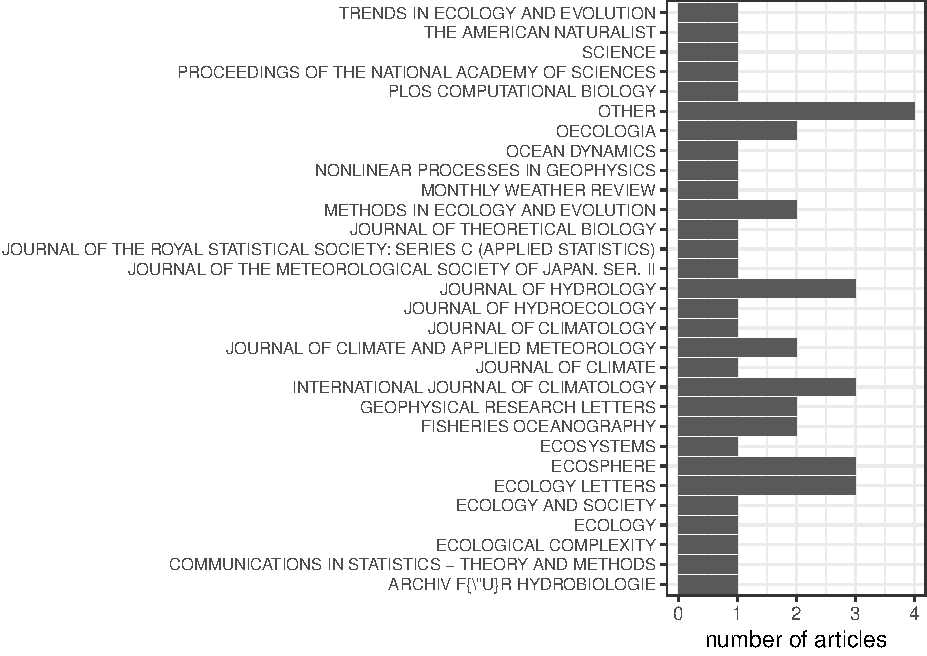
\includegraphics{_myDissertation_files/figure-latex/jrnlDistFig-1.pdf}
\caption{\label{fig:jrnlDistFig}Distribution of identified methods across publications via the literature review.}
\end{figure}
A critical survey of potetial and realized applications of these methods would be useful for highlighting the needs of future research and methodological improvements. Many of the methods presented in Table \ref{tab:methodsMetricsListTab1} have either not been applied to empirical data at all, or were tested only once, often but not always in the article introducing or adapting the methodology (Hawkins et al., 2015). Some methods, especially those dubbed `early warning indicators' (variance, autoregressive model coefficients) have become relativley mainstream in their application to empirical data, despite having been shown to be less robust in noisy and nonlinear systems (Burthe et al., 2016), in systems exhibiting lag-effects (Guttal et al., 2013), and in systems not exhibiting catstrophic shifts (Dutta et al., 2018). Unlike these early warning indicators, fewer efforts have been made to test robustness under these and more simple conditions (Dutta et al., 2018; c.f. Brock \& Carpenter, 2010; Benedetti-Cecchi, Tamburello, Maggi, \& Bulleri, 2015). In addition to the paucity of studies attempting to understand the limitations of these methods, this review suggests that simply identifying the suite of methods used in ecological regime shift detections may be difficult using traditional review methods. Many of the methods metnioned in this review were not identified using a systematic search process in Web of Science and Google Scholar--rather, they were methods of which I was either previously aware and/or highlighted in the few methods reviews (Andersen et al., 2009; Boettiger et al., 2013; Clements \& Ozgul, 2018; Dakos et al., 2015a, 2015b; deYoung et al., 2008; Filatova et al., 2016; Kefi et al., 2014; Litzow \& Hunsicker, 2016; Mantua, 2004; Roberts et al., 2018; S. N. Rodionov, 2005; Scheffer et al., 2015). To facilitate this process, an online, comprehensive database may prove useful to the practical ecologist.

Many of the methods identified in this review have yet to be tested on multiple, empirical datum (see Table \ref{tab:methodsMetricsListTab1}). I categorize the regime detection methods as one of either model-free or model-dependent. Model-free and model-dependent methods are those which do and do not require a mechanistic model to describe the system, respectively. Because many of the model-dependent methods are based on autoregressive modelling apporaches, this is highlighted in the model-dependent section (however most autoregessive models are non-specific).

Model-dependent require a mechanistic (mathematical) representation of the system, models which often carry strict assumptions that are easily violated by empirical systems (Abadi et al., 2010). Model-dependent methods are usefully categorized are used under two contexts: differentiable systems of equations or autoregressive. The methods relying on mechanistic models include model descriptions of systems with many, dynamic and interacting components. For example, models are used to reconstruct trophic food webs where prey or predator collapse induces trophic regime shifts in freshwater lake systems.

Model-free (or metric-based per Dakos, Carpenter, et al., 2012) methods are those which do not require a mathematical represntation of the system. In fact, many require much less knowledge about the system component dynamics and their interactions to calculate a results. The utility of these methods vary with respect to the number of state variables encompassed in the method, and are therefore further categorized as either univariate (using a single dimesion) or multivariable (using but not necessarily requiring multiple dimensions). The most widely used model-free univariate RDMs include descriptive statistics of individual system components (i.e.~univariate), such as variance, skewness, and mean value (Andersen et al., 2009; Mantua, 2004; S. Rodionov \& Overland, 2005). These univariate methods require only very simple calculations, however, their efficacy in empirical systems analysis is controversial. For example, variance (Carpenter \& Brock, 2006) and skewness (of a single variable), oft referred to generally as `leading indicators' or `early-warning indicators' in the literature, has been applied to both theoretical and empirical systems data with varying results.

Hastings \& Wysham (2010a) point out an important feature of using any methods for identifying regime shifts in empirical system data: we only have a single history within which we can compare AND these metrics which depend on the system exhibiting a change in variance or skewness around a mean value before and after a regime shift require hte system to have a smooth potential, rather than one which can manifest complex dynamics (i.e.~non-smooth potential). If we are using RDMs to attempt to forecast and prevent non-smooth or abrupt changes, then there is little justification for relying upon these early warning indicators. Specifcally, these early-warning indicators may be most useful when the system is expected to undergo a transcritical or critical bifurcation before exiting a regime (Lenton, 2011). Hastings \& Wysham (2010a) aptly point out that any realisitic ecological model should incorporate some degree of stochasticity, and when this stochasticity is introduced into the function, the function will likely not be differentiable at the point of the regime shift (Graham \& Tél, 1984). In other words, most (if not all) ecological systems have non-smooth potentials, and many of the current methods for identifying regime shifts assume otherwise, often failing if the assumption is violated.

To make the regime detection measures more available and transparent to the practical ecologist, I recommend the following:
1. consitent use of fewer methods
1. persistent collection and maintenance of baseline data (reference data)
1. an on-line database of all methods
- open-sourced
- linked to the original sources (in ecology and statistics or mathematics)
- linked to applications
1. a critical review of the current state of methods in ecology
- including methodological advancements
- especially highlighting where the method fails to perform
- including historical tracking of specific methods to identify which may need to be retired, rather than resuscitated
1. more empirical applications of these methods (especially of those only tested on toy and experimental data)
1. relation of RDMs in ecology to other fields (computer science, data science, climatology and oceanography)

I suggest (Table \ref{tab:nextStepsTab}) a suite of questions which may be useful in a critical review of the characteristics, rigor, and application potential of methods in the context of ecological regime shift detection.
\begin{longtable}{>{\bfseries}l|>{\raggedright\arraybackslash}p{30em}}
\caption{\label{tab:nextStepsTab}Potential questions for a comprehensive review of the ecological regime detection metrics literature.}\\
\toprule
Type & Questions\\
\midrule
Methodological & Does the method assume smooth potential?\\
 & Does the regime shift need to be identified *a priori*?\\
 & What are the major assumptions about the distribution of the original data?\\
 & Does the method explicitly assume the system/variable is stationary?\\
 & Does the performance of the method change with non-stationarity?\\
\addlinespace
 & Can the method handle unstructured data?\\
 & Can the method handle multiple regime shifts?\\
 & What types of regime shifts can the method detect (e.g., stochastic resonance, slow-fast cycles, noise-induced transition)?\\
 & Is it a model- or metric-based method?\\
 & Does it have forecasting potential?\\
\addlinespace
 & Can the method handle uneven sampling?\\
 & What are the minimum data requirements (resolution, extent, number of observations)?\\
 & How does the method handle missing data (e.g., new invasions)?\\
 & Does the method assume Eulerian or Lagrangian processes?\\
Ecological & Does the system *have* smooth potential?\\
\addlinespace
 & Has the method been tested on empirical data? If so, to what rigor?\\
 & What is the impact of losing state variables on long-term predictions (e.g., species extinction)?\\
 & Can the method identify drivers?\\
 & What assumptions does the method make about the system?\\
 & What types of regime shifts are possible in the system?\\
\addlinespace
 & Are regime shift(s) suspected *a priori*?\\
 & What lag(s) exist in the data (system)?\\
 & Would a positive forecast change management action?\\
 & Do predictions translate to other systems?\\
 & Can we interpolate data if necessary? If so, what does this mean for inference?\\
\addlinespace
 & In which discipline(s) beyond ecology has the method been tested?\\
\bottomrule
\end{longtable}
\hypertarget{fiGuide}{%
\chapter{Decoupling the Calculation of Fisher Information}\label{fiGuide}}

\emph{This chapter is intended for submission to the publication \emph{Methods in Ecology and Evolution}.\footnote{Co-authors include: N.B. Price, A.J. Tyre, D.G. Angeler, T. Eason, D. Twidwell, and C.R. Allen}}

\hypertarget{abstract-1}{%
\section{Abstract}\label{abstract-1}}

Ecological regime shifts are increasingly prevalent in the Anthropocene. The number of methods proposed to detect these shifts are on the rise, yet few are capable detecting regime shifts without a priori knowledge of the shift, and fewer are capable of handling high-dimensional, multivariate and noisy data. A variation of Fisher Information has been proposed as a method for detecting changes in the ``orderliness'' of ecological systems data. Although this method is described and applied in numerous published studies, its calculation and the concepts behind its calculation are not clear. Here, I succinctly describe this calculation using a two-species predator-prey model. Importantly, I demonstrate that the actual equation for calculating Fisher Information metric comprises fewer steps than was previously described, by decoupling the dimensionality-reduction component from the actual Fisher Information calculation component. I hope this work will serve as a reference for those seeking to understand Fisher Information in the context of ecological systems and regime shifts, and will stimulate further research of the efficacy of these composite regime shift detection metrics..

\hypertarget{introduction-1}{%
\section{Introduction}\label{introduction-1}}

Changes in the feedback(s) governing ecosystem processes can trigger unexpected and sometimes undesirable responses in environmental conditions (Scheffer, Carpenter, Foley, Folke, \& Walker, 2001; Walther et al., 2002). Ecologists often refer to such changes as regime shifts, but this term is used interchangeably in the literature with state change, state transition, or alternative state (Andersen et al., 2009). Climate change and globalization are triggering novel and unexpected changes in ecosystems (Hughes, 1994; Parmesan, 2006; Scheffer et al., 2001; Walther et al., 2002), and the rapidity with which these changes occur make predictive modeling difficult. Although detecting regime shifts is increasingly difficult as we increase the extent and complexity of the system in question (Jorgensen \& Svirezhev, 2004), advances in the collection and analysis of ecological data (La Sorte et al.~2018) may improve our ability to detect impending regime shifts in time for intervention (Carpenter et al., 2011; deYoung et al., 2008; Groffman et al., 2006; Jorgensen \& Svirezhev, 2004; Sagarin \& Pauchard, 2012; Wolkovich, Cook, McLauchlan, \& Davies, 2014).

Numerous quantitative approaches have been proposed as regime shift detection methods (Clements \& Ozgul, 2016 ; Mantua, 2004; S. Rodionov \& Overland, 2005, p. @andersen\_ecological\_2009), but few are consistently applied to terrestrial ecological data (deYoung et al., 2008). I broadly classify these methods as either model-based or model-free {[}Boettiger \& Hastings (2012); Hastings \& Wysham (2010b); Dakos, Carpenter, et al. (2012). Model-based methods use mathematical (mechanistic) representations of the system (Hefley, Tyre, \& Blankenship, 2013), which often carrying strict assumptions that are easily violated by dynamic systems such as ecosystems (Abadi et al., 2010). Further, model misspecification may yield spurious results (Perretti, Munch, \& Sugihara, 2013). Model-free (or metric-based, per Dakos, Carpenter, et al., 2012) regime detection methods require fewer assumptions to implement than do model-based methods, and typically require much less knowledge (if any) about system component interactions. The most widely used model-free methods include both descriptive statistics of individual system components, such as variance, skewness, and mean value (Andersen et al., 2009; Mantua, 2004; S. Rodionov \& Overland, 2005) and composite measures of multiple variables, notably principal components analysis (Möllmann, Folke, Edwards, \& Conversi, 2015; Petersen et al., 2008), clustering algorithms (Beaugrand, 2004), and variance index (Brock \& Carpenter, 2006).

\hypertarget{fisher-information-as-a-regime-detection-method}{%
\subsection{Fisher Information as a Regime Detection Method}\label{fisher-information-as-a-regime-detection-method}}

A method which has been more recently applied in the analysis of ecological and social-ecological systems is Fisher Information (Cabezas \& Fath, 2002; Karunanithi, Cabezas, Frieden, \& Pawlowski, 2008). As a multivariate, model-free method, Fisher Information integrates the information present in the entire data of a system and distills this complexity into a single metric. This allows Fisher Information to capture ecosystem dynamics with higher accuracy than univariate-based metrics, which frequently fail to detect regime changes (Burthe et al., 2016). However, despite the potential of this method its mathematical underpinnings -- specifically its calculation and the concepts behind its calculation-- are not clear. In this paper, I address this knowledge gap. I first provide an overview of the method and highlight the need to account for scaling properties, an inherent feature in complex systems. I then succinctly describe the decoupling of the dimensionality-reduction component from the actual Fisher Information calculation component using a two-species predator-prey model. I finally discuss the results from a theoretical viewpoint and its practical utility for predicting regime shifts, an increasing concern motivated by current rates of fast ecological change.

\hypertarget{the-sustainable-regimes-hypothesis}{%
\subsection{The Sustainable Regimes Hypothesis}\label{the-sustainable-regimes-hypothesis}}

Fisher Information (hereafter, FI; Fisher, 1922) is a model-free, composite measure of any number of variables, and is proposed as an early warning signal for ecological regime shift detection and as a measure of system sustainability (Eason \& Cabezas, 2012; Eason et al., 2014a; Karunanithi et al., 2008; Mayer, Pawlowski, Fath, \& Cabezas, 2007). Three definitions of FI in this context exist: (i) a measure of the ability of the data to estimate a parameter, (ii) the amount of information extracted from a set of measurements (Frieden, 1990; Roy Frieden, 1998), and (iii) a measure representing the dynamic order/organization of a system (Cabezas \& Fath, 2002). Although definitions (i) and (ii) are widely applied in the statistical and physical sciences, I focus on definition (iii) as it is gaining traction as a tool to analyze used in the context ofeco ecological systems analysisresponses to fast environmental change. The application of FI to complex ecological systems was posed as part of the ``Sustainable Regimes Hypothesis,'' stating a system is sustainable, or is in a stable dynamic state, if over some period of time the average value of FI does not drastically change (Cabezas \& Fath, 2002). This concept can be described using an ecological example. Consider the simple diffusion of a population released from a point source at \(t=0\). This process can be described by a bivariate normal distribution, \(p(x,y|t)\). As the time since release, \(t\), increases, the spread of the distribution, \(p(x,y|t)\), disperses because the animals have moved further from the release location. As the animal moves away from the release location, the potential area within which it currently occupies will increase with time. In this example, FI will decrease in value as t increases because \(p(x,y|t)\) contains less information (higher uncertainty) about where the animals will be located. If we assume constant dispersal, as \(t\rightarrow\infty\) the animals will be relatively uniformly distributed across the environment and \(p(x,y|t)\) will carry no information about the location of the animals. Consequently, as \(t\rightarrow\infty\) FI approaches zero (no information). Per the Sustainable Regimes Hypothesis (Cabezas \& Fath, 2002), this example system is not in a stable dynamic state over the range of \(t\), since FI decreases with time.

Conversely, if a population following a simple logistic growth model, \(\frac{dN}{dt}=rN(1-\frac{N}{K})\), varies around some carrying capacity, K, and the average system parameters (\(r\), \(K\), and their variances \(\sigma_r, \sigma_k\)) are stationary, then the logarithm of the population size should follow a normal distribution, \(N ~ normal(\mu,\sigma)\). In this situation, the FI measured over any selected window of time will be relatively constant and, per the Sustainable Regimes Hypothesis, indicates the system is in a stable dynamic state. Further, this Hypothesis posits that a perturbation to N will also not affect FI so long as the perturbation occurs with a stationary probability distribution and if the perturbation does not change the distributions of \(r\) and \(K\).

\hypertarget{fisher-information-requires-dimension-reduction}{%
\subsection{Fisher Information Requires Dimension Reduction}\label{fisher-information-requires-dimension-reduction}}

An important feature of the FI method is that it requires a complete reduction in dimensionality (i.e., from \(>1\) to \(1\) system component). For example, a recent application of Fisher Information to empirical data condensed a species pool from 109 species time series into a 1-dimensional time series (Spanbauer et al., 2014). A reduction in dimensionality, i.e.~condensing multivariate data into a single metric, of over two orders of magnitude likely involves a large loss of relevant information, raising the questions of what information is preserved during the dimensionality reduction step in calculating FI, what is lost, and whether this is important. Other dimension reduction techniques, e.g., principal component analysis (PCA) and redundancy analysis (RDA), attempt to preserve the variance of the data, and the number of components scales with the dimensionality of the data (i.e.~they are scale explicit). In contrast, by reducing entirely the dimensionality of the data, the FI method does not identify which features of the data are preserved, and the dimensionality does not scale with the dimensionality of the original data.

\hypertarget{aims}{%
\subsection{Aims}\label{aims}}

The key contribution of this study is that I decouple the dimensionality reduction step of the FI method (Step 1) from the statistical analysis step (Step 2). By isolating the dimensionality reduction step, we can evaluate it based on its own merits and relate it to more well-known and established methods of dimensionality reduction. By isolating the statistical analysis step, one can better understand how Fisher Information is calculated on the single-dimensional data. I believe that this decoupled approach will eliminate some confusion regarding the calculation of FI, allowing interested researchers to readily evaluate the merits of this method. To facilitate our explanation of the method, I reproduce the predator-prey analysis used in (Fath, Cabezas, \& Pawlowski, 2003; Mayer et al., 2007), then induce a ``regime shift'' into the model. I hope this work will serve as a useful explanation of the FI metric for those seeking to understand it in the ecological regime shift context and will stimulate research using this and other multivariate, model-free, and composite measures to understand ecological regime shifts.

\hypertarget{methods-1}{%
\section{Methods}\label{methods-1}}

\hypertarget{predator-prey-model-system}{%
\subsection{Predator-Prey Model System}\label{predator-prey-model-system}}

Our model system is a two-species predator-prey model (Eq. \eqref{eq:predprey}; Fath et al., 2003; Frieden \& Gatenby, 2007; Mayer et al., 2007), hereafter referred to as the ``model system'':
\begin{equation} 
  dx_1 = g_{1}x_{1}(1-\frac{x_1}{k})- \frac{l_{12} x_{1} x_{2}}{1+\beta x_{1}} \\
  dx_2 = \frac{g_{21}x_1 x_2}{1+\beta x_1} - m_2 x_2)
  \label{eq:predprey}
\end{equation}
The specified parameters for the model system are \(g_1=m_2=1\),\(l_{12}=g_{12}= 0.01\) ,\(k=625\) ,and \(\beta=0.005\) (Fath et al., 2003; Frieden \& Gatenby, 2007; Mayer et al., 2007). The initial conditions (predator and prey abundances,) for the model system were not provided in the original references (Fath et al., 2003; Mayer et al., 2007). I used package \texttt{deSolve} in Program R (version 3.3.2) to solve the model system (Eq. Eq. \eqref{eq:predprey}), finding \$x\_1 = 277.781\$5 and \(x_2= 174.551\) to provide reasonable results. A complete cycle of this system corresponds to \(~11.145\) time units.

\hypertarget{inducing-a-regime-shift}{%
\subsection{Inducing a Regime Shift}\label{inducing-a-regime-shift}}

Mayer et al. (2007) calculated FI for a predator-prey system for several discrete values of carrying capacity of prey. The results of this study showed that FI was different for systems with different carrying capacities (\(K\)). However, this study did not address the central question of \textbf{FI behavior during a regime shift}. As an extension of the original study, I simulated a regime shift by modeling an abrupt decline in carrying capacity, \(k\). I assume \(k\) is described by Eq. \eqref{eq:mayerCase} where \(k_1\) is the initial carrying capacity, \(k_2\) is the final carrying capacity, \(t_shift\) is the time the regime shift occurred, and \(\alpha\) is the parameter controlling the rate (slope) of the regime shift. The hyperbolic tangent function (see Eq. \eqref{eq:mayerCase}) simulates a smooth and continuous change in \(k\) while still allowing for the regime shift to occur rapidly. I incorporate the change in \(k\) into our system of differential equations by defining the rate of change in \(k\), \(k'(t)\), given by (Eq. \eqref{eq:mayerCase}). I assume \(k_1=800\) and \(k_2=625\), values corresponding to the range of carrying capacities explored by Mayer et al. (2007). I simulated a time series of 600 time units, introducing a regime change after 200 time units, and \(\alpha=0.05\).
\begin{equation}  
  k(t) = k_1  - 0.5(k_1-k_2)(\tanh(\alpha (t-t^*))+1) \\ 
  k'(t) = 0.5\alpha (k_1-k_2)(\tanh(\alpha(t-t^*))^2 +1) 
\label{eq:mayerCase}
\end{equation}
\hypertarget{decoupling-the-steps-for-calculating-fisher-information}{%
\subsection{Decoupling the Steps for Calculating Fisher Information}\label{decoupling-the-steps-for-calculating-fisher-information}}

Two methods exist for calculating Fisher Information (FI) as applied to ecological systems data to which I refer the ``derivatives-based'' method (first appearing in Cabezas \& Fath (2002) and the binning" method (first appearing in Karunanithi et al. (2008)). Although the binning method is proposed as an alternative to the derivatives-based method for handling noisy and sparse data, our decoupling method reveals it may be an unnecessary method. Therefore, I focus on only the derivatives-based method for explaining the theoretical basis for the FI method. The general form of FI can be found in (Fath et al., 2003; Mayer et al., 2007) and I refer the reader to (Cabezas \& Fath, 2002).

\_\_Step 1: Dimensionality Reduction. The key idea of the dimensionality reduction step is to calculate the Euclidean distance travelled in phase space. In phase space, each coordinate axis corresponds to a system state variable (e.g., number of predators and number of prey). The state of the model system over time describes a path or trajectory through phase space. The distance travelled represents the cumulative change in state relative to an arbitrary starting point in time. For the model system, the distance travelled in phase space can be obtained by solving the differential equation given by Eq. \eqref{eq:s}
\begin{equation}  
\frac{ds}{dt} = \sqrt(\frac{dx_1}{dt}^2 + \frac{dx_2}{dt}^2)
\label{eq:s}
\end{equation}
The original motivation for the dimensionality reduction step is that, under restrictive conditions, there is a one-to-one mapping between the state of the system (\(s\)), defined in a multidimensional phase space, and the distance travelled, a one-dimensional summary (Cabezas \& Fath, 2002). To relate this abstract idea to a more familiar situation, we draw an analogy between the path traced by the system in phase space and the path of a car over the course of a trip. The distance travelled by the car over time is related to the position of the car. Given the route of the car, we could determine the location of the car at any point in time if we know how far it has travelled. However, the distance travelled provides no information about the proximity of locations (i.e., system states). For example, two points in phase space may be arbitrarily close, but the distance travelled would be different if these system states occur at different points in time. Moreover, if the system revisits the same state twice then the one-to-one mapping breaks down and a single state maps to potentially very different values of distance travelled.

What is preserved in the calculation of distance travelled is the rate of change of the system (e.g., the speed and acceleration of the car). The rate of change of the system is the first derivative of the distance travelled in phase space. This is an important point because the concept of a ``regime shift'' is often associated with the idea of a sudden change in system state. Therefore, it may not be unreasonable to employ a dimensionality reduction procedure that preserves these system dynamics.

\textbf{Step 2: Statistical Analysis.} The product of \textbf{Step 1} is a one-dimensional time series of what I call ``distance travelled'', \(s\), (in phase space). The variable \(s\) is referred to as ``Fisher variable s'' and ``represent{[}s{]} a particular state of phase space'' in the FI literature (Mayer et al., 2007). I believe distance travelled (\(s\)) is more descriptive than ``Fisher Variable s'' and avoids confusing the state of the system, defined in multiple dimensionsby the multivariate data , with the one-dimensional summary. Using this measure, we next calculate the probability of observing the system in a particular state by assuming a one-to-one mapping between distance travelled and the system state. That is, we calculate the probability of observing the system at a particular distance, \(p(s)\), along the trajectory for some period of time from 0 to \(t_end\). The time at which we observe the system is assumed to be a random variable, \(T_{obs} \sim Uniform(0,t_end)\). This approach assumes the system is deterministic and is observed without error. However, the observed distance travelled by the system, \(s\), is a random variable because it is a function of the random observation time.

Importantly, the probability of observing the system at a particular value of s increases if the system is changing slowly at that point in time. That is \(p(s)\) is inversely proportional to the system rate of change, \(s'\). Mathematically, the distance travelled in phase space, \(s\), is a monotonically increasing function of time and we assume it is differentiable. Therefore, the probability density function of the distance travelled is \(p(s)=\frac{1}{T}\frac{1}{s'}\), where \(s'=\frac{ds}{dt}\) is the speed (or velocity) of \(s\), and \(T\) is the time interval over which the system was observed (\(t_{start}\)-\(t_{end}\)). We note that \(p(s)\) is simply a constant multiplied by the inverse of the speed of the system.

The original motivation for the FI calculation as applied to ecological systems was the hypothesis that ``since Fisher Information is a measure of the variation'' it is also ``an indicator of system order, and thus system sustainability'' (Cabezas \& Fath, 2002). Equation \eqref{eq:fiAdapted} is a general form of FI and Equation \eqref{eq:fiDerivs} is the form used in the derivative-based method for FI (see eq. 7.3b and 7.12 in Mayer et al., 2007). To better understand the FI calculation, note that Eq.\eqref{eq:fiDerivs} is, in part, a measure of the gradient content of the probability density function. As the probability density function becomes flatter, the FI value will decrease. In this way, the FI calculation is closely related to the variance. In fact, the FI value for a normal distribution calculated according to Eq. \eqref{eq:fiDerivs} is simply one over the variance. It is also important to note that FI is zero for a uniform distribution, as the probability density function is flat. Note also that FI goes approaches \(\inf\) if the system is not changing over some period of time (Eq. \eqref{eq:fiDerivs}).
\begin{equation} 
    I = \int \frac{ds}{p(s)}\left[\frac{dp(s)}{ds}\right]^2  \\
    \label{eq:fiAdapted}
\end{equation}
\begin{equation}
    I=\frac{1}{T}\int_0^Tdt\left[\frac{s''^2}{s'^4}\right]^2 \\
  \label{eq:fiDerivs}
\end{equation}
\begin{figure}
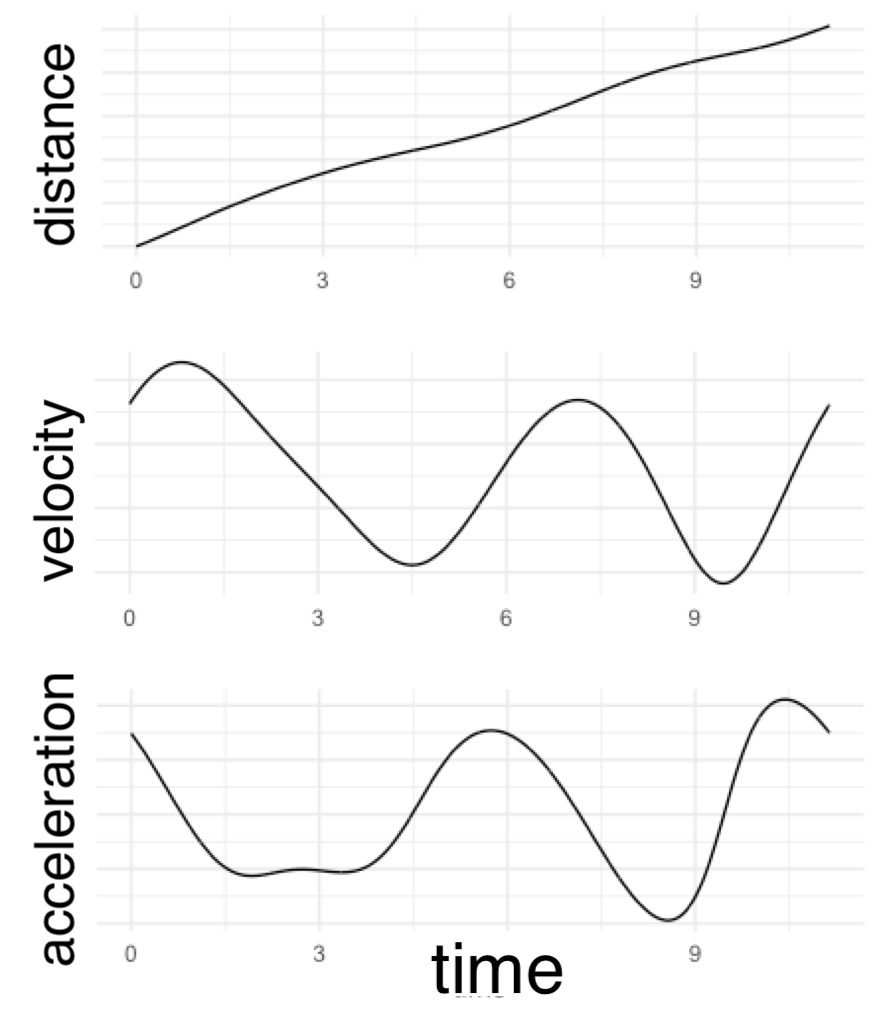
\includegraphics[width=0.95\linewidth]{/Users/jessicaburnett/Documents/GitHub/myDissertation//chapterFiles/fiGuide/figures/distSppedAccel} \caption{From top to bottom, distance traveled in phase space, speed tangential to system trajectory, acceleration tangential to system trajectory.}\label{fig:distSpeedAccel}
\end{figure}
\#\#Results
Distance travelled (\(s\)), speed (\(\frac{ds}{dt}\)), and acceleration (\(\frac{d^2 s}{dt^2}\)) capture the dynamics of the model system {[}Eq. \eqref{eq:predprey}; Fig. @ref(fig:distSpeedAccel{]}. I simulated a regime shift in the carrying capacity of this model system, at approximately \(t=200\) (Fig. \ref{fig:kByTime}). The location of this regime shift with respect to the system trajectory in phase space over the entire simulated time period is shown in (Fig. \ref{fig:kTrajectories}). Although a slight change is captured by \(s\) (Figure 4) at the location of this regime shift, it is not pronounced. Although the distance travelled, \(s\) (Fig. \ref{fig:sOverTime}) changes fairly smoothly around the location of the regime shift, the system exhibits a steep decline in speed ds/dt soon after the induced regime shift (Fig. \ref{fig:dsdtOverTime}).

I calculated FI for the distribution of \(s\) over a series of non-overlapping time windows. According to Mayer et al. (2007) the length of the time window should be equal to one system period such that FI is constant for a periodic system, however, the system periods are not identical before, during, and after the regime shift. Therefore, I performed two separate calculations of FI using window sizes corresponding to the initial (when \(t<200\)) and the final (\(t>200\)) periods of the system (\(winsize = 13.061\) and \(11.135\) time units, respectively). Using these window sizes the drop in FI at the regime shift initiation is bigger than the magnitude of the fluctuations preceding it (Fig. \ref{fig:fiOverTime}).
\begin{figure}
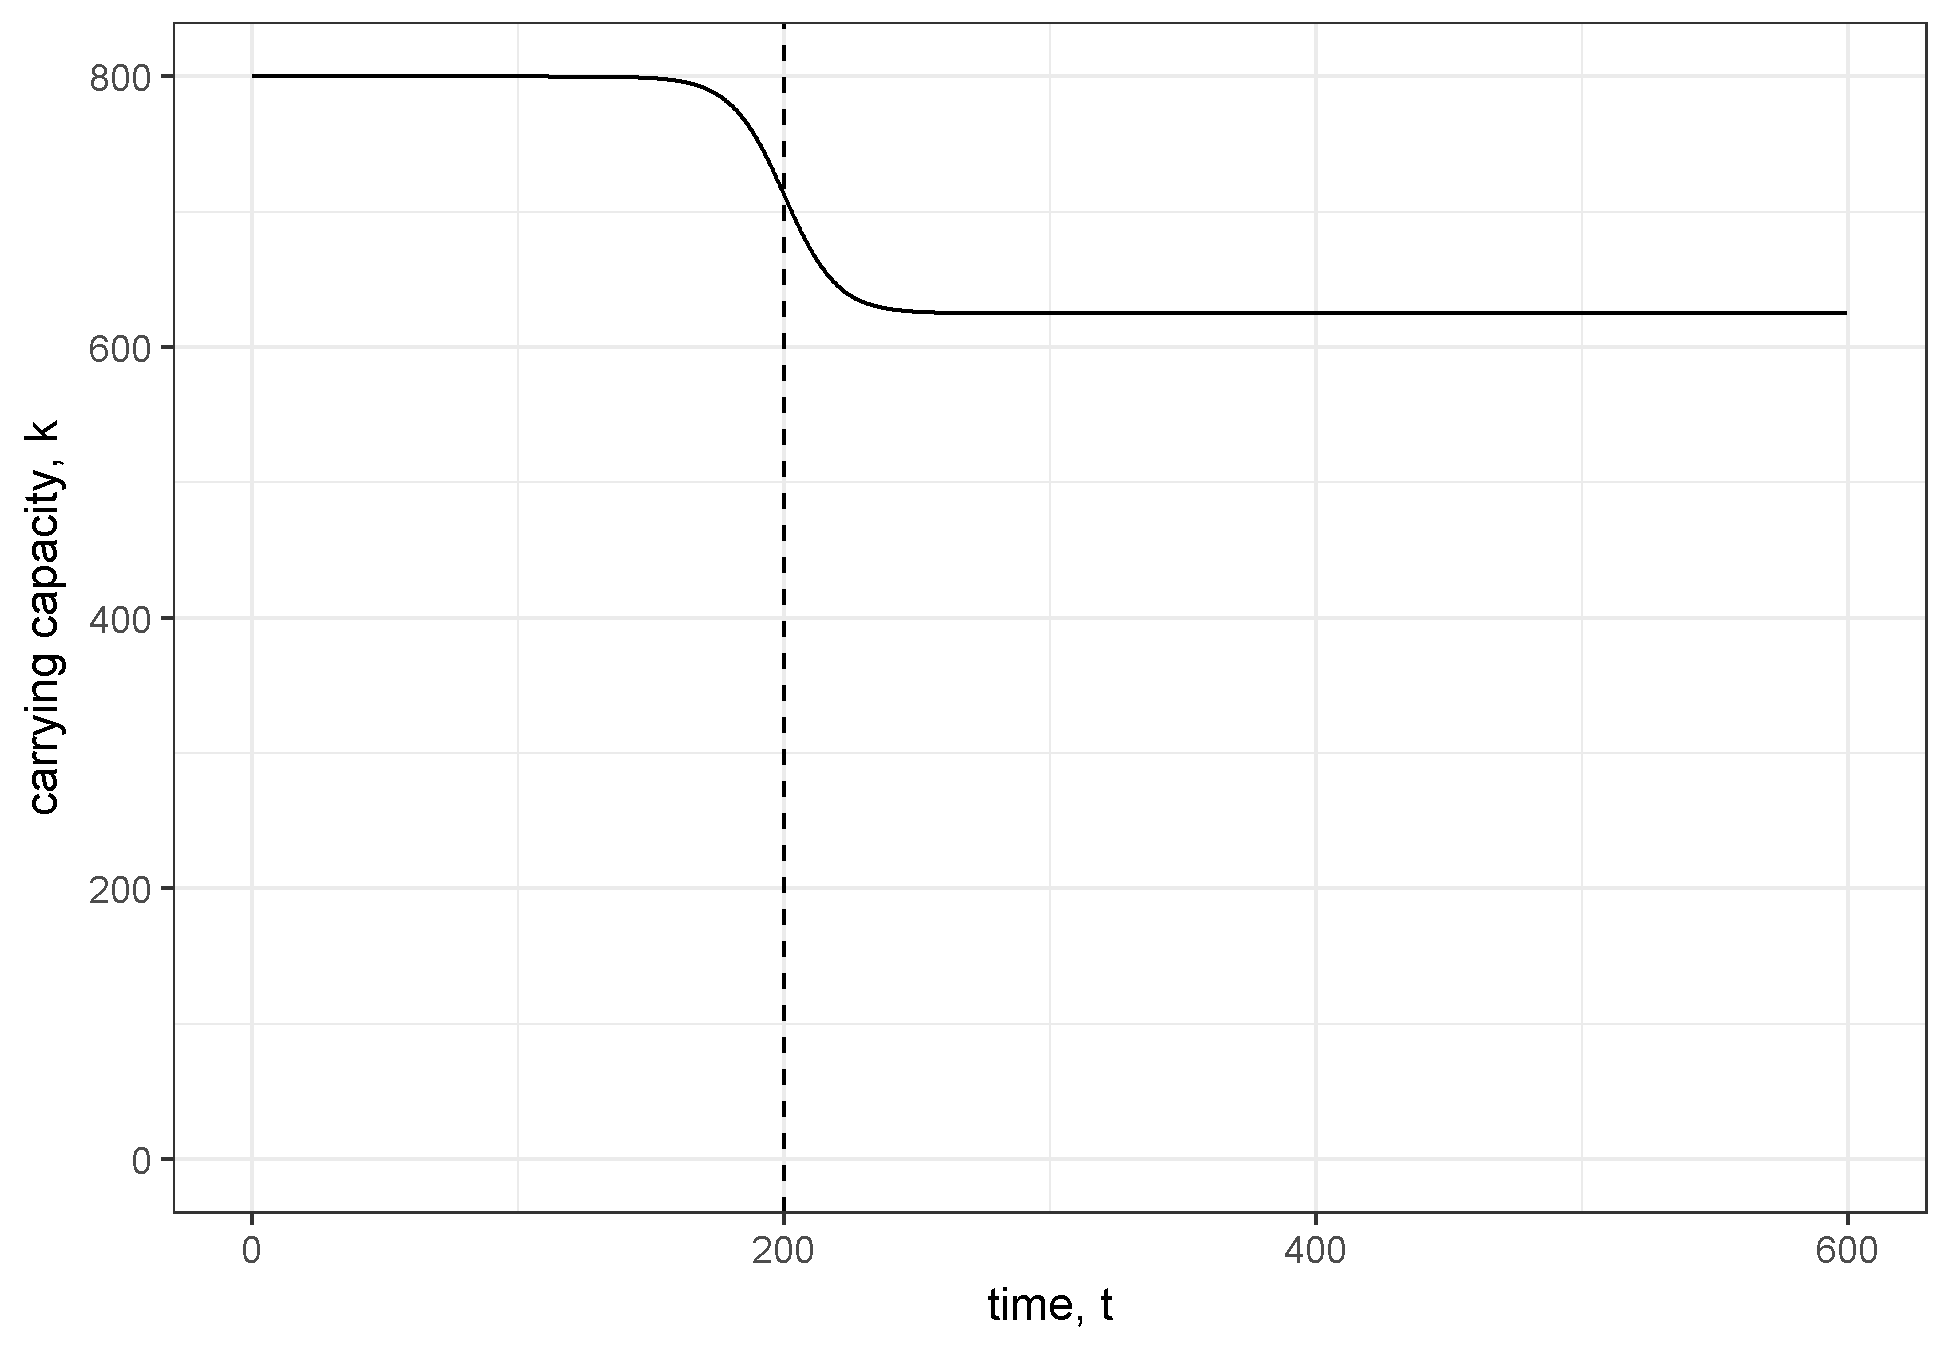
\includegraphics[width=0.95\linewidth]{./chapterFiles/fiGuide/figures/kByTime} \caption{Carrying capacity over time with a regime shift occuring around time 200.}\label{fig:kByTime}
\end{figure}
\begin{figure}
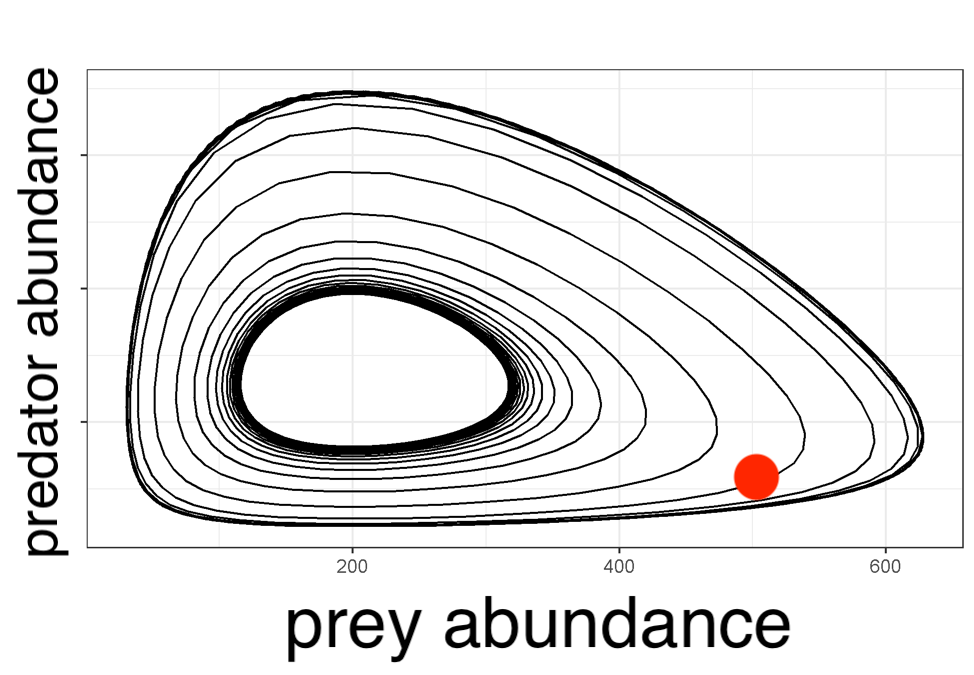
\includegraphics[width=0.95\linewidth]{/Users/jessicaburnett/Documents/GitHub/myDissertation//chapterFiles/fiGuide/figures/kTrajectories} \caption{Phase space plot of system trajectories for different values of k}\label{fig:kTrajectories}
\end{figure}
\begin{figure}
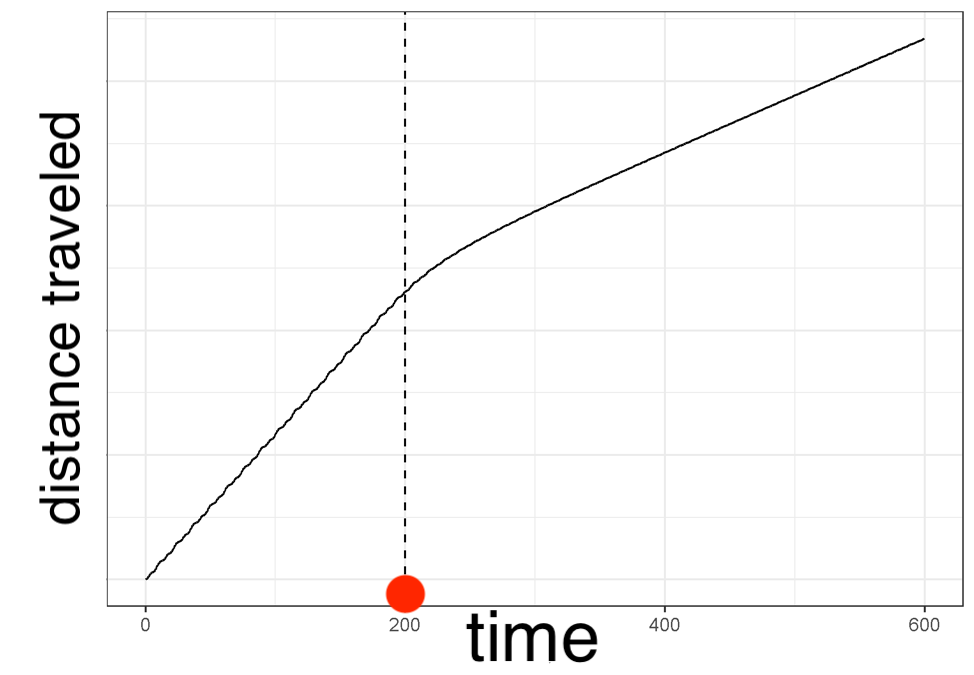
\includegraphics[width=0.95\linewidth]{./chapterFiles/fiGuide/figures/sOverTime} \caption{Distance travelled in phase space over time. Dashed vertical line at time 200 indicates location of regime shift.}\label{fig:sOverTime}
\end{figure}
\hypertarget{discussion-1}{%
\section{Discussion}\label{discussion-1}}

Part of the appeal of the FI method of regime shift detection is that it provides a 1-dimensional visual summary of system ``orderliness''. However, I have demonstrated that the dimensionality reduction step can be performed separately from the calculation of FI. The rate of change of the system (velocity, \(\frac{ds}{dt}\)\}), on which FI method is based, is also a 1-dimensional quantity. In the simple predator-prey example, calculating and plotting FI did not provide a clear benefit over simply plotting the system rate of change directly. I suggest that future research uncouple the dimensionality reduction step and the FI calculation step in order to better illustrate the benefits of the FI method relative to dimensionality reduction alone.
\begin{figure}
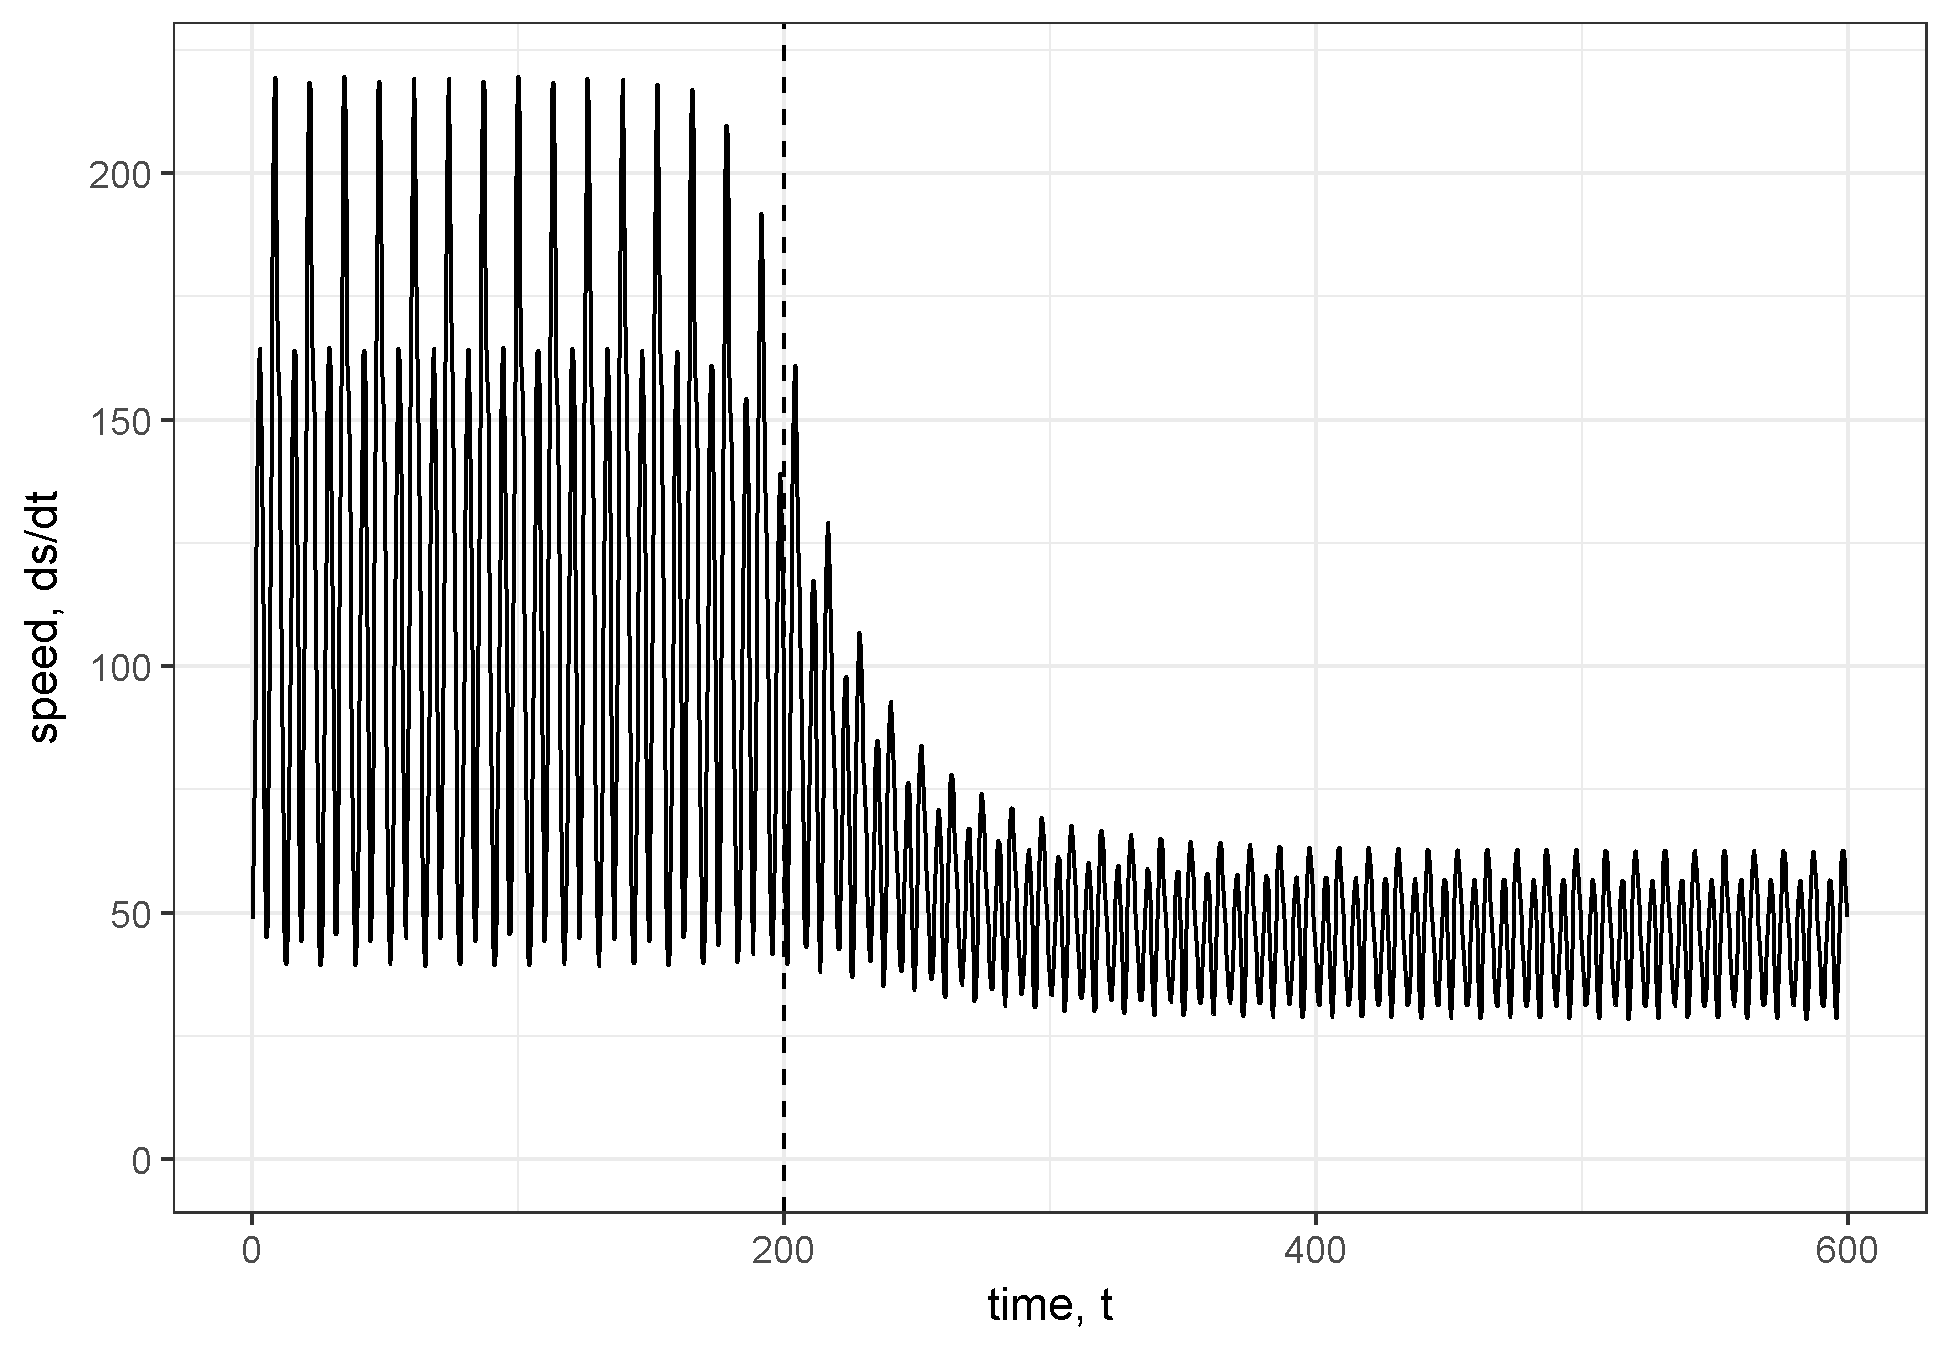
\includegraphics[width=0.95\linewidth]{./chapterFiles/fiGuide/figures/dsdtOverTime} \caption{Speed of the system (rate of change, velocity) in phase space. Dashed vertical line at time 200 indicates location of regime shift.}\label{fig:dsdtOverTime}
\end{figure}
In the predator-prey example, I assumed the data was free from observation error. Despite these ideal conditions, the estimated FI had high variation and the results depended on the size of the time window used in the calculation. This issue arises because the period of the cyclic system is changing during the regime shift such that it is difficult to find a single window size that works well for the entire time series. Mayer et al. (2007) describe this as a ``confounding issue'' related to ``sorting out the FI signal of regime change from that originating from natural cycles'' and suggest using a time window that is large enough to include several periods. However, in the absence of a quantitative decision rule defining what changes in FI indicate regime shifts, it is difficult to separate the signal in the FI metric from the noise due to fluctuations in the natural cycles. Further research is needed to define quantitative decision rules for what changes in FI constitute a regime shift.

The example used in this study is unrealistic in that I assume no measurement error and therefore focus on the ``derivatives-based'' method of calculating FI. However, our analysis also has implications for the ``binning'' method of calculating FI that was later developed for high-dimension noisy data (Karunanithi et al. (2008)). Rather than attempting to estimate the rate of change of each system component (e.g., hundreds of species) and combining these estimates to get the total system rate of change, I suggest an approach where the dimensionality of the data is first reduced by calculating distance travelled in phases-pace and then only a single rate of change is estimated. The advantage of this approach is that for an n-dimensional system it only requires the estimation of one derivative rather than n-derivatives . The drawback to this approach is that noisy observations will likely introduce some bias into the estimate of the system rate of change. Nonetheless, I believe this approach is worth exploring due to its simplicity relative to the ``binning'' method.
\begin{figure}
\includegraphics[width=0.95\linewidth]{./chapterFiles/fiGuide/figures/fiOverTime} \caption{Fisher Information calculated for non-overlapping time windows. Two different window sizes were used as indicated by color. Dashed vertical line at time 200 indicates approximate location of regime shift.}\label{fig:fiOverTime}
\end{figure}
The Fisher Information of an \(n\)-dimensional system is a vector of unitless values which can only be compared within a dataset (e.g., within a single community time series) and interpreting FI is still largely a qualitative effort (Fath et al., 2003; Mantua, 2004), not unlike most regime detection methods {[}Ch. \ref{rdmReview}{]}. When the FI of a system is increasing, the system is said to be moving toward a more orderly state, and most studies of FI propose that sharp changes in FI, regardless of the directionality of the change, may indicate a regime shift (Cabezas \& Fath, 2002; Karunanithi et al., 2008; Spanbauer et al., 2014). Although the aforementioned and numerous other works interpret FI in this context (e.g., Eason et al., 2014a; Eason \& Cabezas, 2012), I suggest future work which clearly identifies the ecological significance of the Fisher Information metric and its significance within the ecological regime shift paradigm.

\hypertarget{acknowledgements}{%
\section{Acknowledgements}\label{acknowledgements}}

I thank H. Cabezas and B. Roy Frieden for early discussions regarding the development of Fisher Information, and T.J. Hefley for comments on an earlier draft. This work was funded by the U.S. Department of Defense's Strategic Environmental Research and Development Program (project ID: RC-2510).

\hypertarget{fisherSpatial}{%
\chapter{An application of Fisher Information to spatially-explicit avian community data}\label{fisherSpatial}}

\hypertarget{introduction-2}{%
\section{Introduction}\label{introduction-2}}

Ecosystems are open, dynamical systems which arguably cannot be fully represented by deterministic models. Despite the complexity of most ecological systems, some patterns have emerged in certain statistical mechanics of ecological observations. An uptick in recent years of studies of \textbf{regime shifts} (\ref{glossary}) in ecology has spurred an increase in the number of `new' methods for detecting ecological regime shifts (\ref{rdmReview}), some of which are proposed as indicators of `spatial' regime shifts (Butitta, Carpenter, Loken, Pace, \& Stanley, 2017, pp. @kefi2014early, @sundstrom2017detecting, @guttal2009spatial, @brock\_variance\_2006).

As defined in \ref{glossary}, a regime shift is largely considered an abrupt and persistent change in a system's structure or functioning. Following this definition and without any associated \textbf{pressures} \ref{glossary}, it is not yet clear whether identifying a `spatial regime' using a snapshot of a system (a single or short period of time relative to the time scale of the pressure) is pragmatic. One spatial regime detection measure (hereafter, SRDM) is variance (Brock \& Carpenter, 2006), despite its controversial applicability to temporal data (Burthe et al., 2016, pp. @dutta2018robustness, @perretti2012regime, @sommer2017generic, @bestelmeyer\_analysis\_2011). By assuming that variance increases across space prior to a `regime' shift, one can calculate the variability across a landscape.

Defining the spatial regime shift is important since observations of non-random spatial processes (e.g., land cover), could manifest as either rapid shift (e.g.~an ecotone) or a gradual change (slow mixing along a gradient). Consequently, and because most RDMs signal abrupt change, only the former may be identified as ``regime shifts'' using SRDMs. For the concept of spatial regimes to be ecologically useful, potential pressures must be associated with system structure over space \emph{and} time. Additionally and perhaps more importantly, the processes driving the observed information (drivers, pressures ) should be such that a statistically identified regime shift will roughly correspond with the time scale on which the pressure(s) operate.

Although it is suggested that statistical and pragmatic models and methods are advanced more rapidly by bottom-up approaches, i.e.~case studies (see DeAngelis \& Yurek, 2017), to my knowledge no studies have yet to test the rigor of SRDMs using spatially-explicit empirical data. The objective of this chapter is to determine the utility of Fisher Information {[}Eq. \eqref{eq:fiDerivs}{]} as a spatial regime detection measure. This chapter is also supported by original software developed for implementation in Program R, which is publicly available {[}see Appendix \ref{regimeDetectionMeasures}{]}.
\begin{figure}
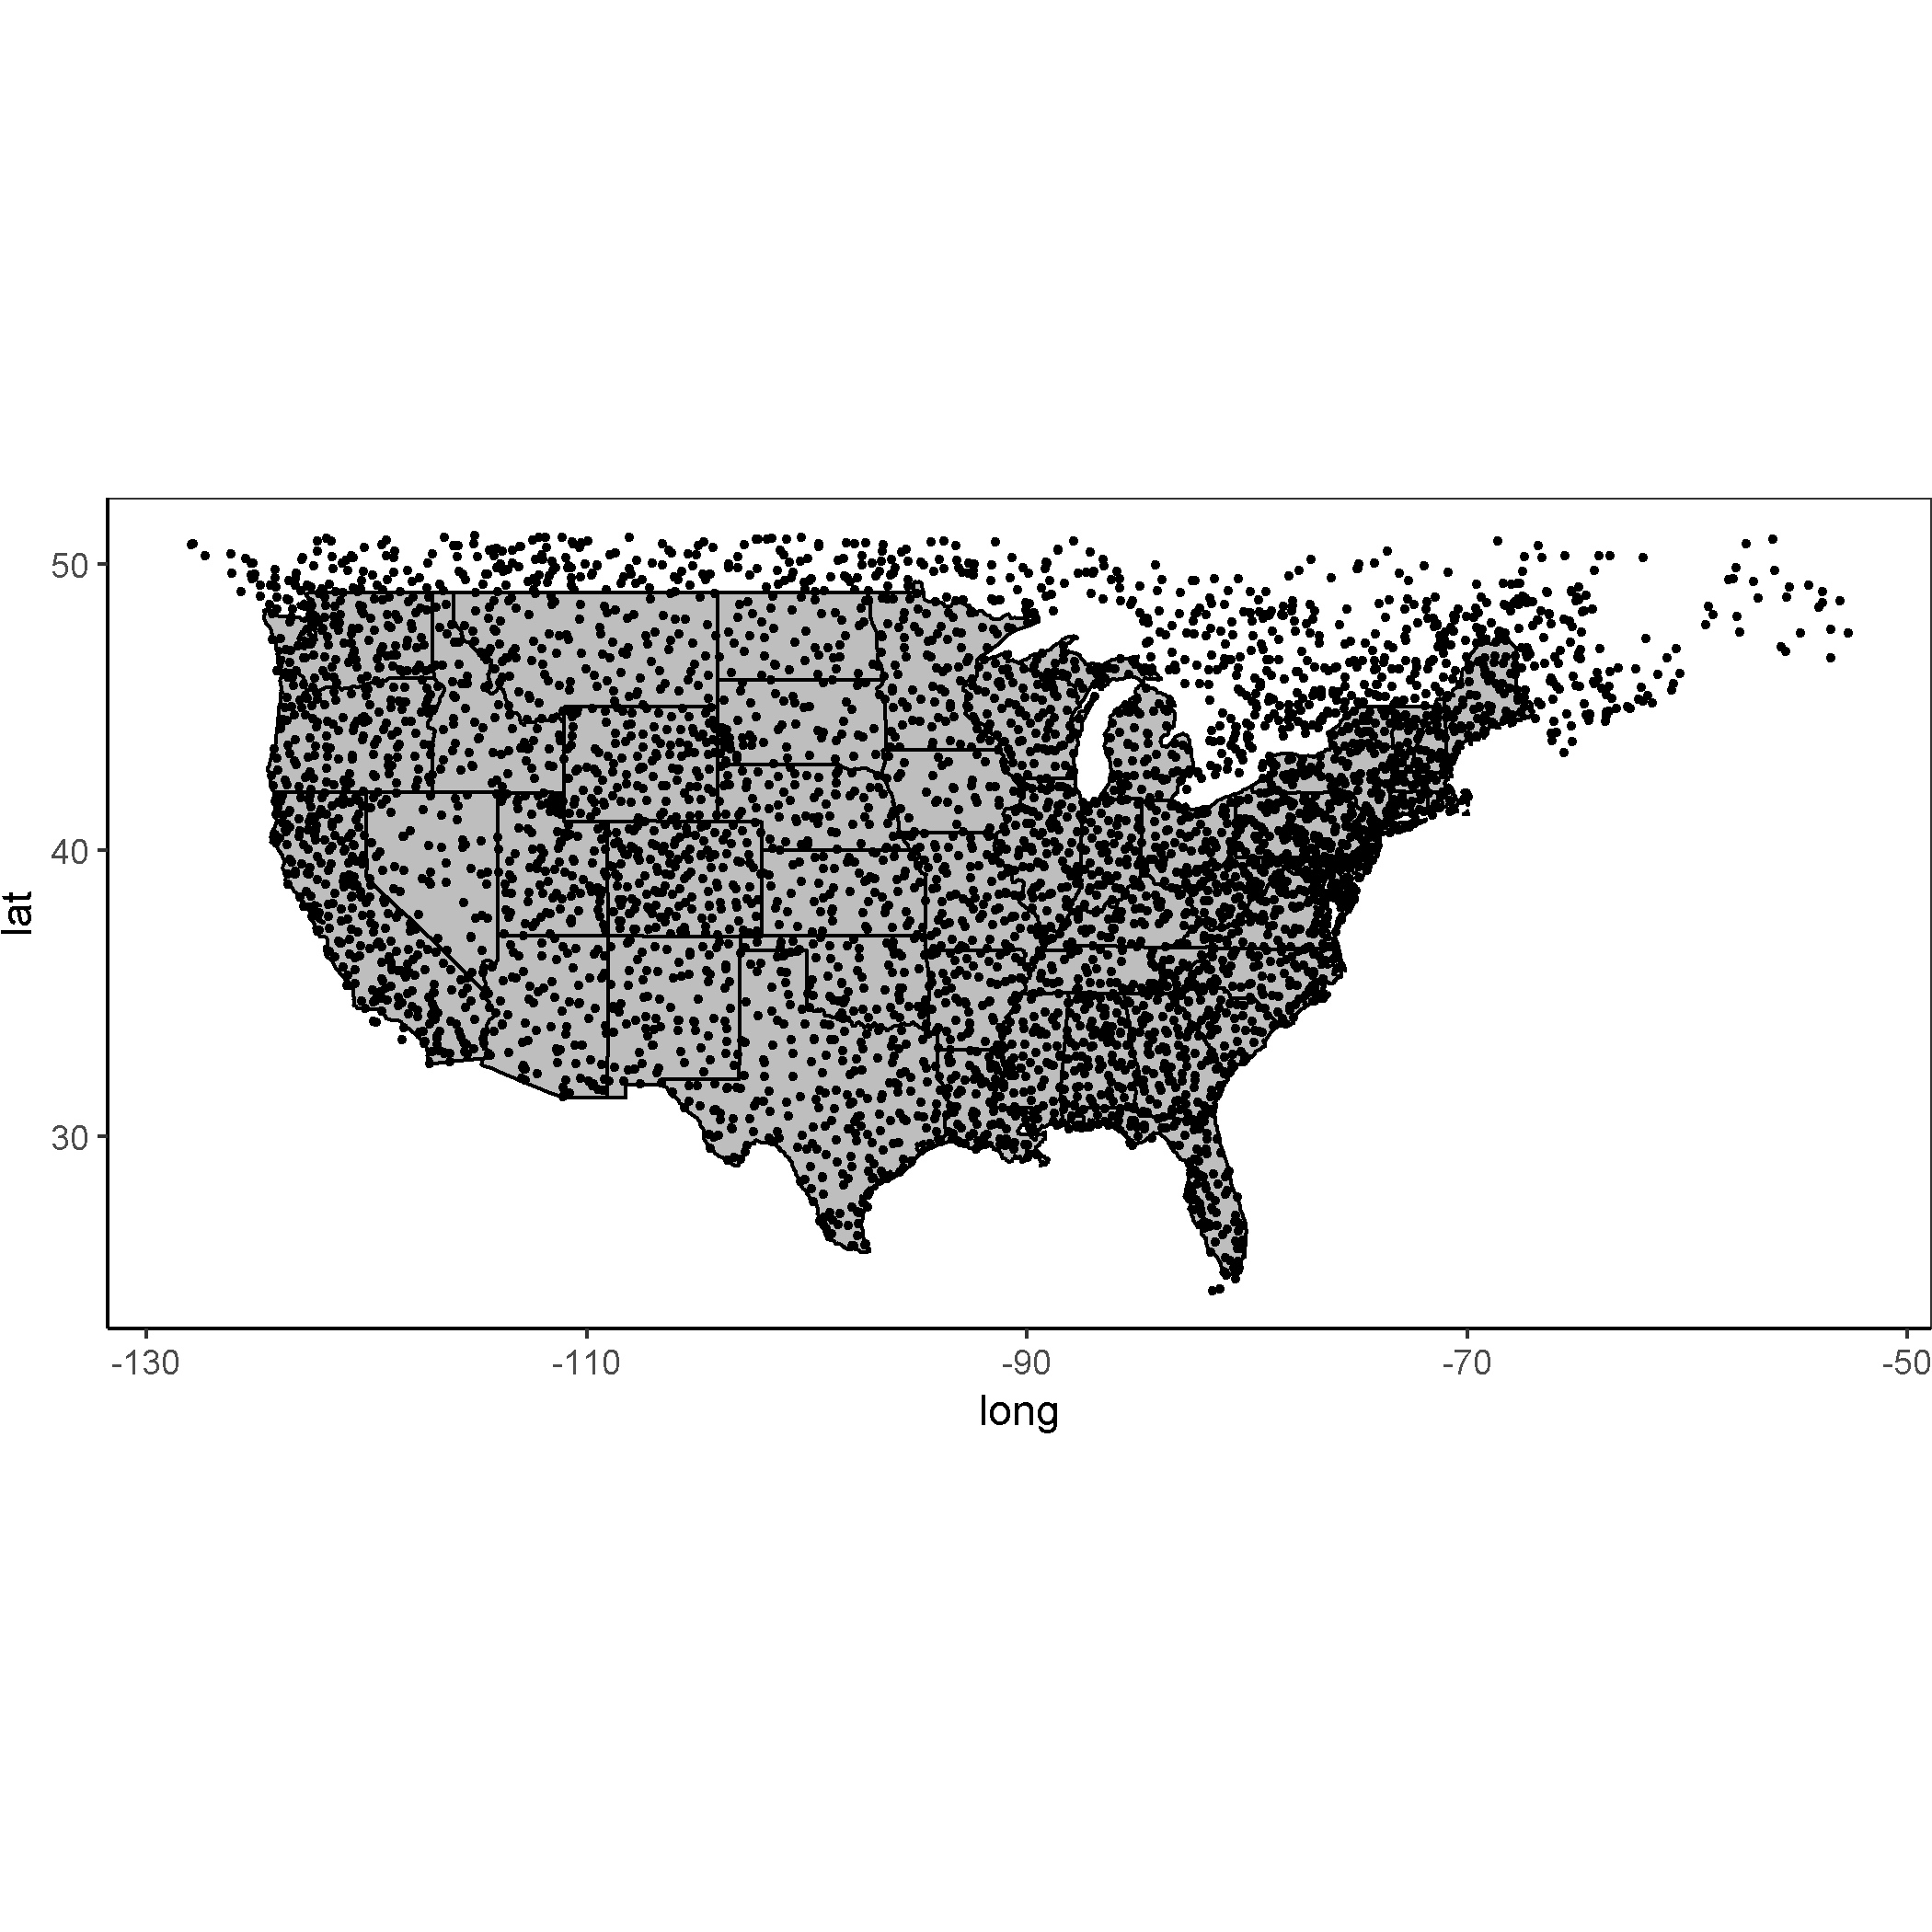
\includegraphics[width=29.17in]{./chapterFiles/fisherSpatial/figures/figsCalledInDiss/bbsRoutesUsed} \caption{Locations of Breeding Bird Survey routes sampled between 1966 and 2017.}\label{fig:bbsPoints}
\end{figure}
\hypertarget{data-and-methods}{%
\section{Data and methods}\label{data-and-methods}}

\hypertarget{data-north-american-breeding-bird-communities}{%
\subsection{Data: North American breeding bird communities}\label{data-north-american-breeding-bird-communities}}

I use community abundance data from long-term monitoring programs to identify spatial and temporal regimes using the Fisher Information (FI) derivatives method (see Eq. \eqref{eq:fiDerivs}). The NABBS trains citizen scientist volunteers to annually collect data using a standardized roadside, single observer point count protocol and has been collecting data regularly across North America (\ref{fig:bbsPoints}) since 1966. The roadside surveys consist of 50 point counts (by sight and sound) along an approximately 24.5 mile stretch of road. Due to strict reliane on volunteers, some routes are not covered every year. Additionally, some routes are moved or discontinued, and some routes are not sampled in a given year. Route-year combinations which are missing years but are not discontinued are treated as missing data. Although NABBS volunteers identify all species as possible, persistent biases exist in this protocol. To reduce the influence of potential sampling bias, I removed waterfowl, waders, and shore species (AOU species codes 0000 through 2880).

\hypertarget{study-area}{%
\subsection{Study area}\label{study-area}}

Although the NABBS conducts surveys throughout much of North America, I limited analyses to the continental United States and parts of southern Canada. NABBS coverage of the boreal forests of Canada are sparse in space, and many routes in Mexico have fewer than 25 years of observations.
\begin{figure}
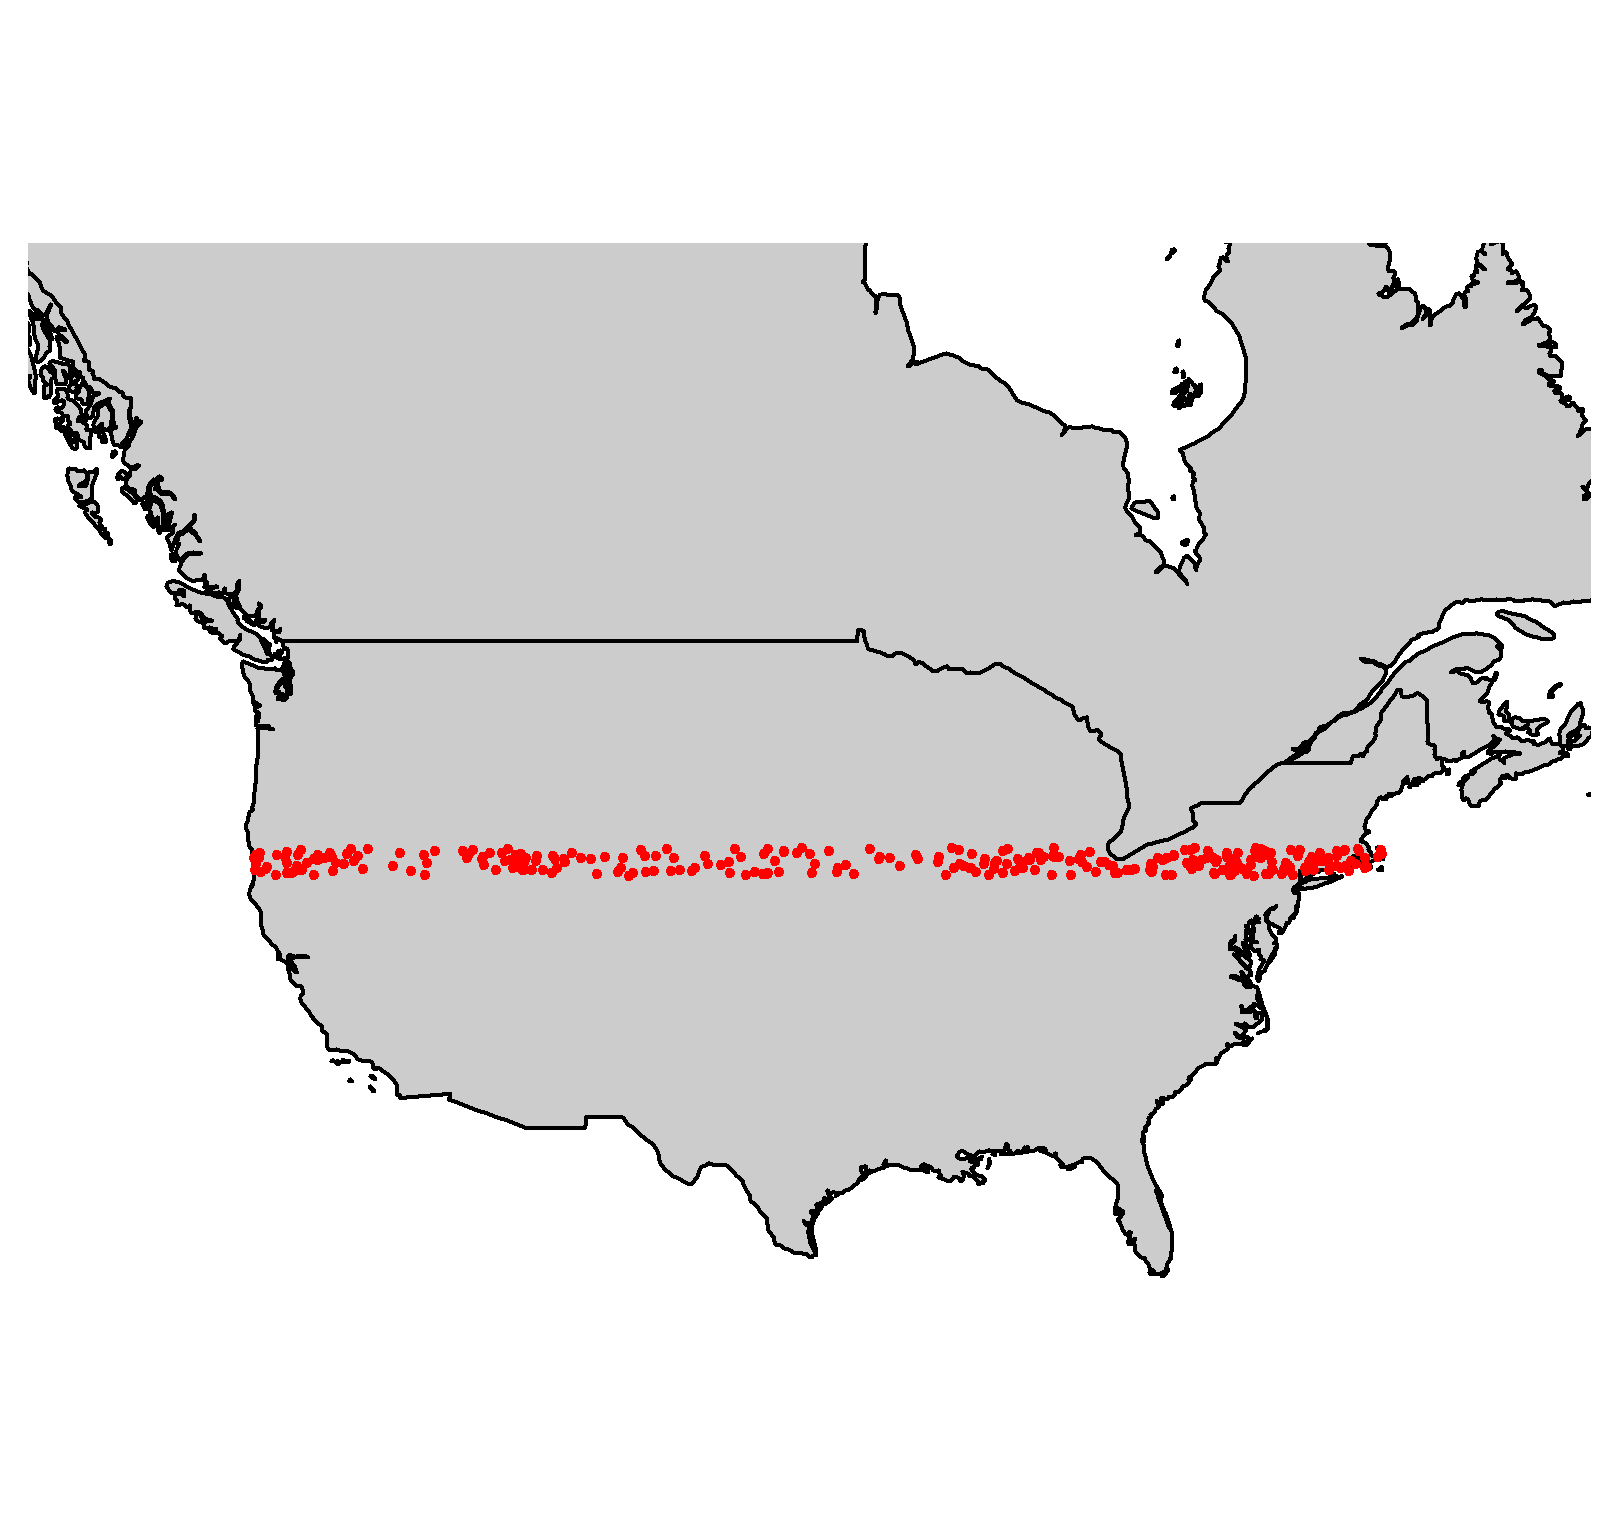
\includegraphics[width=0.85\linewidth]{./chapterFiles/fisherSpatial/figures/figsCalledInDiss/transectSamplingEx_1row} \caption{A single East-West transect of Breeding Bird Survey routes used to calculate the Fisher Information.}\label{fig:ewRouteMap}
\end{figure}
\hypertarget{focal-military-base}{%
\subsubsection{Focal military base}\label{focal-military-base}}

The Mission of the US Department of Defense is to provide military forces to deter war and protect the security of the country, and a primary objective of individual military bases is to maintain military readiness. To maintain readiness, military bases strictly monitor and manage their natural resources. Military bases vary in size and nature, and are heterogeneously distributed across the continental United States (See Fig. \ref{fig:ewRouteMap}). The spread of these bases (Fig. \ref{fig:milBases}), coupled with the top-down management of base-level natural resources presumably influences the inherent difficulties associated with collaborative management within and across military bases and other natural resource management groups (e.g., state management agencies, non-profit environmental groups.

Much like other actively managed landscapes, miltiary bases are typically surrounded by non- or improperly-managed lands. Natural resource managers of military bases face environmental pressures within and surrounding their properties, yet their primary objectives are very different. Natural resource managers of military bases, whose primary objective is to maintain military readiness, are especially concerned with if and how broad-scale external forcings might influence their lands. Prominent concerns include invasive species, wildlife disease, and federally protected species (personal communication with Department of Defense natural resource managers at Eglin Air Force and Fort Riley military bases). For these reasons, natural resource managers attempt to create buffers along their perimeters (e.g., live fire/ammunitions suppression, wide fire breaks). Identifying the proximity of military bases to historic and modern ecological shifts may provide insight into the effectiveness of their natural resource management efforts.
\begin{figure}

{\centering 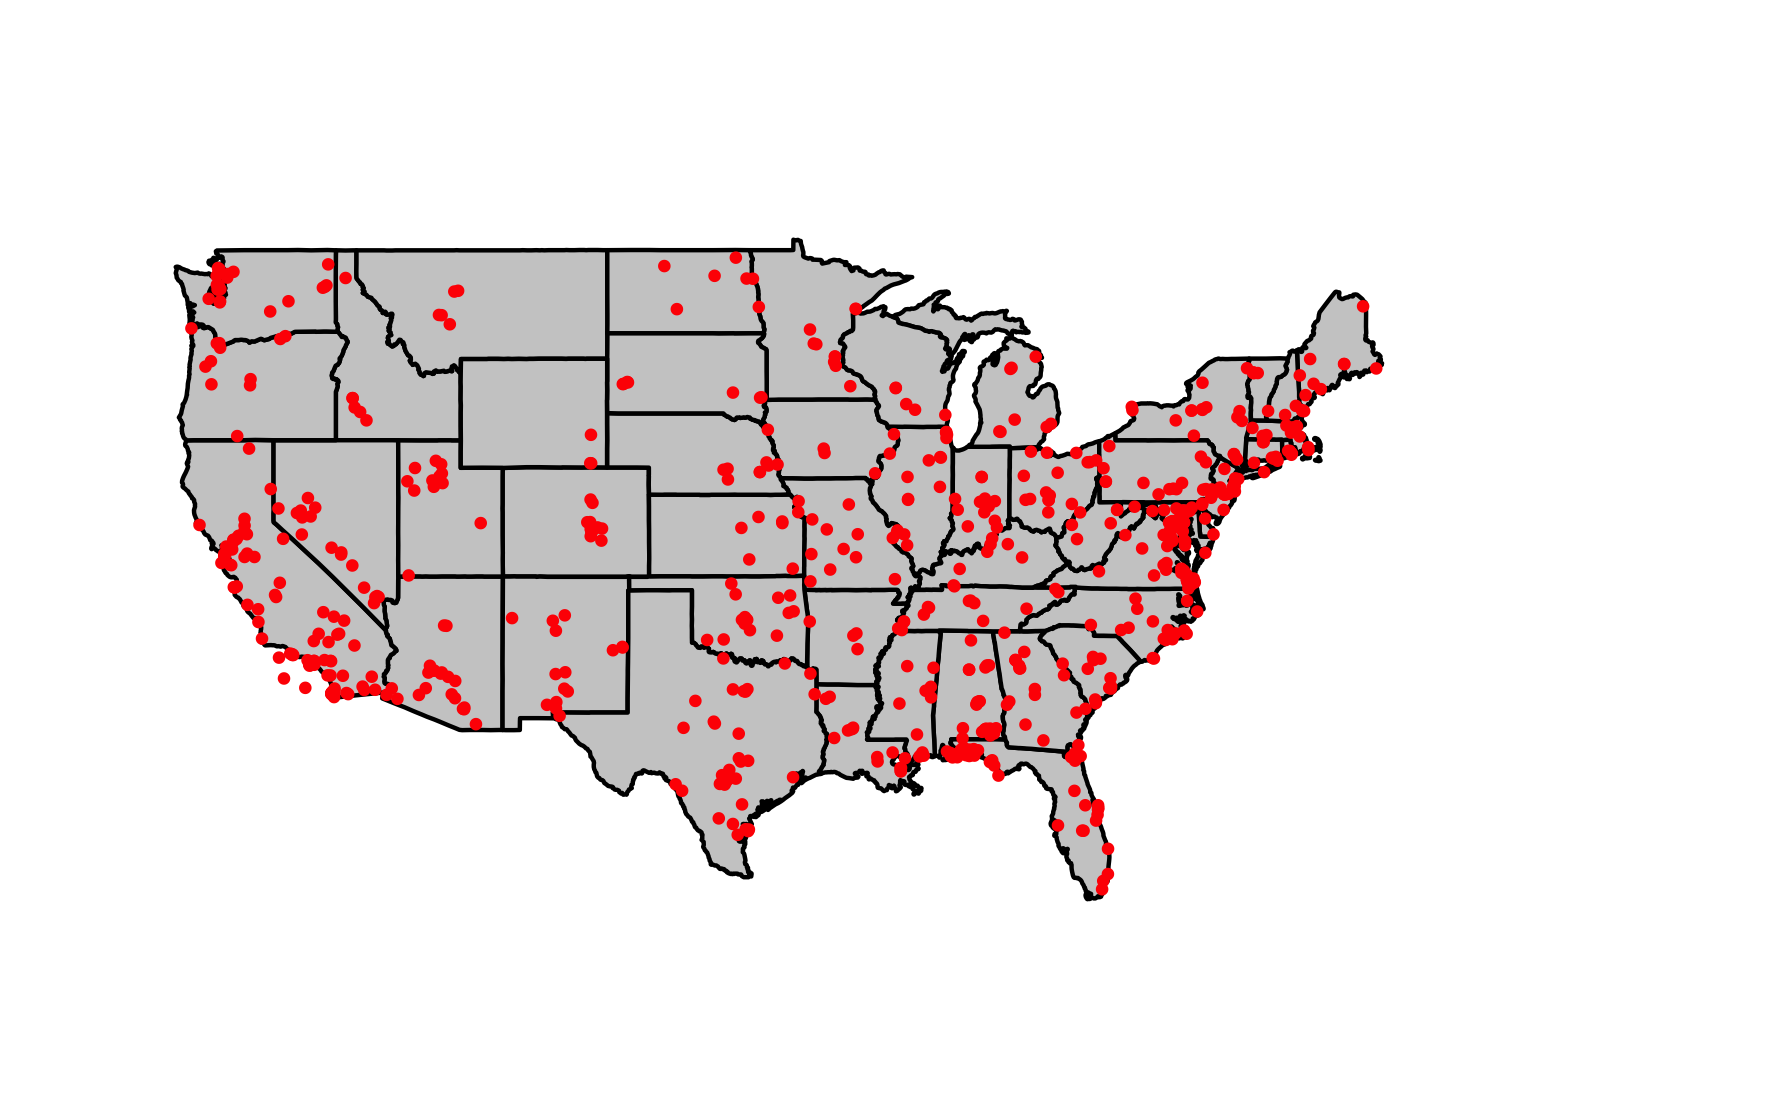
\includegraphics[width=0.85\linewidth]{./chapterFiles/fisherSpatial/figures/figsCalledInDiss/milBases} 

}

\caption{Locations of U.S. military bases in our study area.}\label{fig:milBases}
\end{figure}
The NABBS routes chosen for analyses in this Chapter lie within or near Fort Riley military base (located at approximately \(39.110474^{\circ}\), \(-96.809677^{\circ}\); Kansas, USA). Fort Riley (Fig. \ref{fig:basesOfInterestMap}) is a useful reference site for this study. Woody encroachment of the Central Great Plains over the last century has triggered shifts in dominant vegetative cover and diversity (Ratajczak et al.~2012) in the area surrounding Fort Riley military base (e.g., Van Auken 2009). This phenomena should present itself as a regime boundary should Fisher Information be a robust regime shift detection method.
\begin{figure}

{\centering 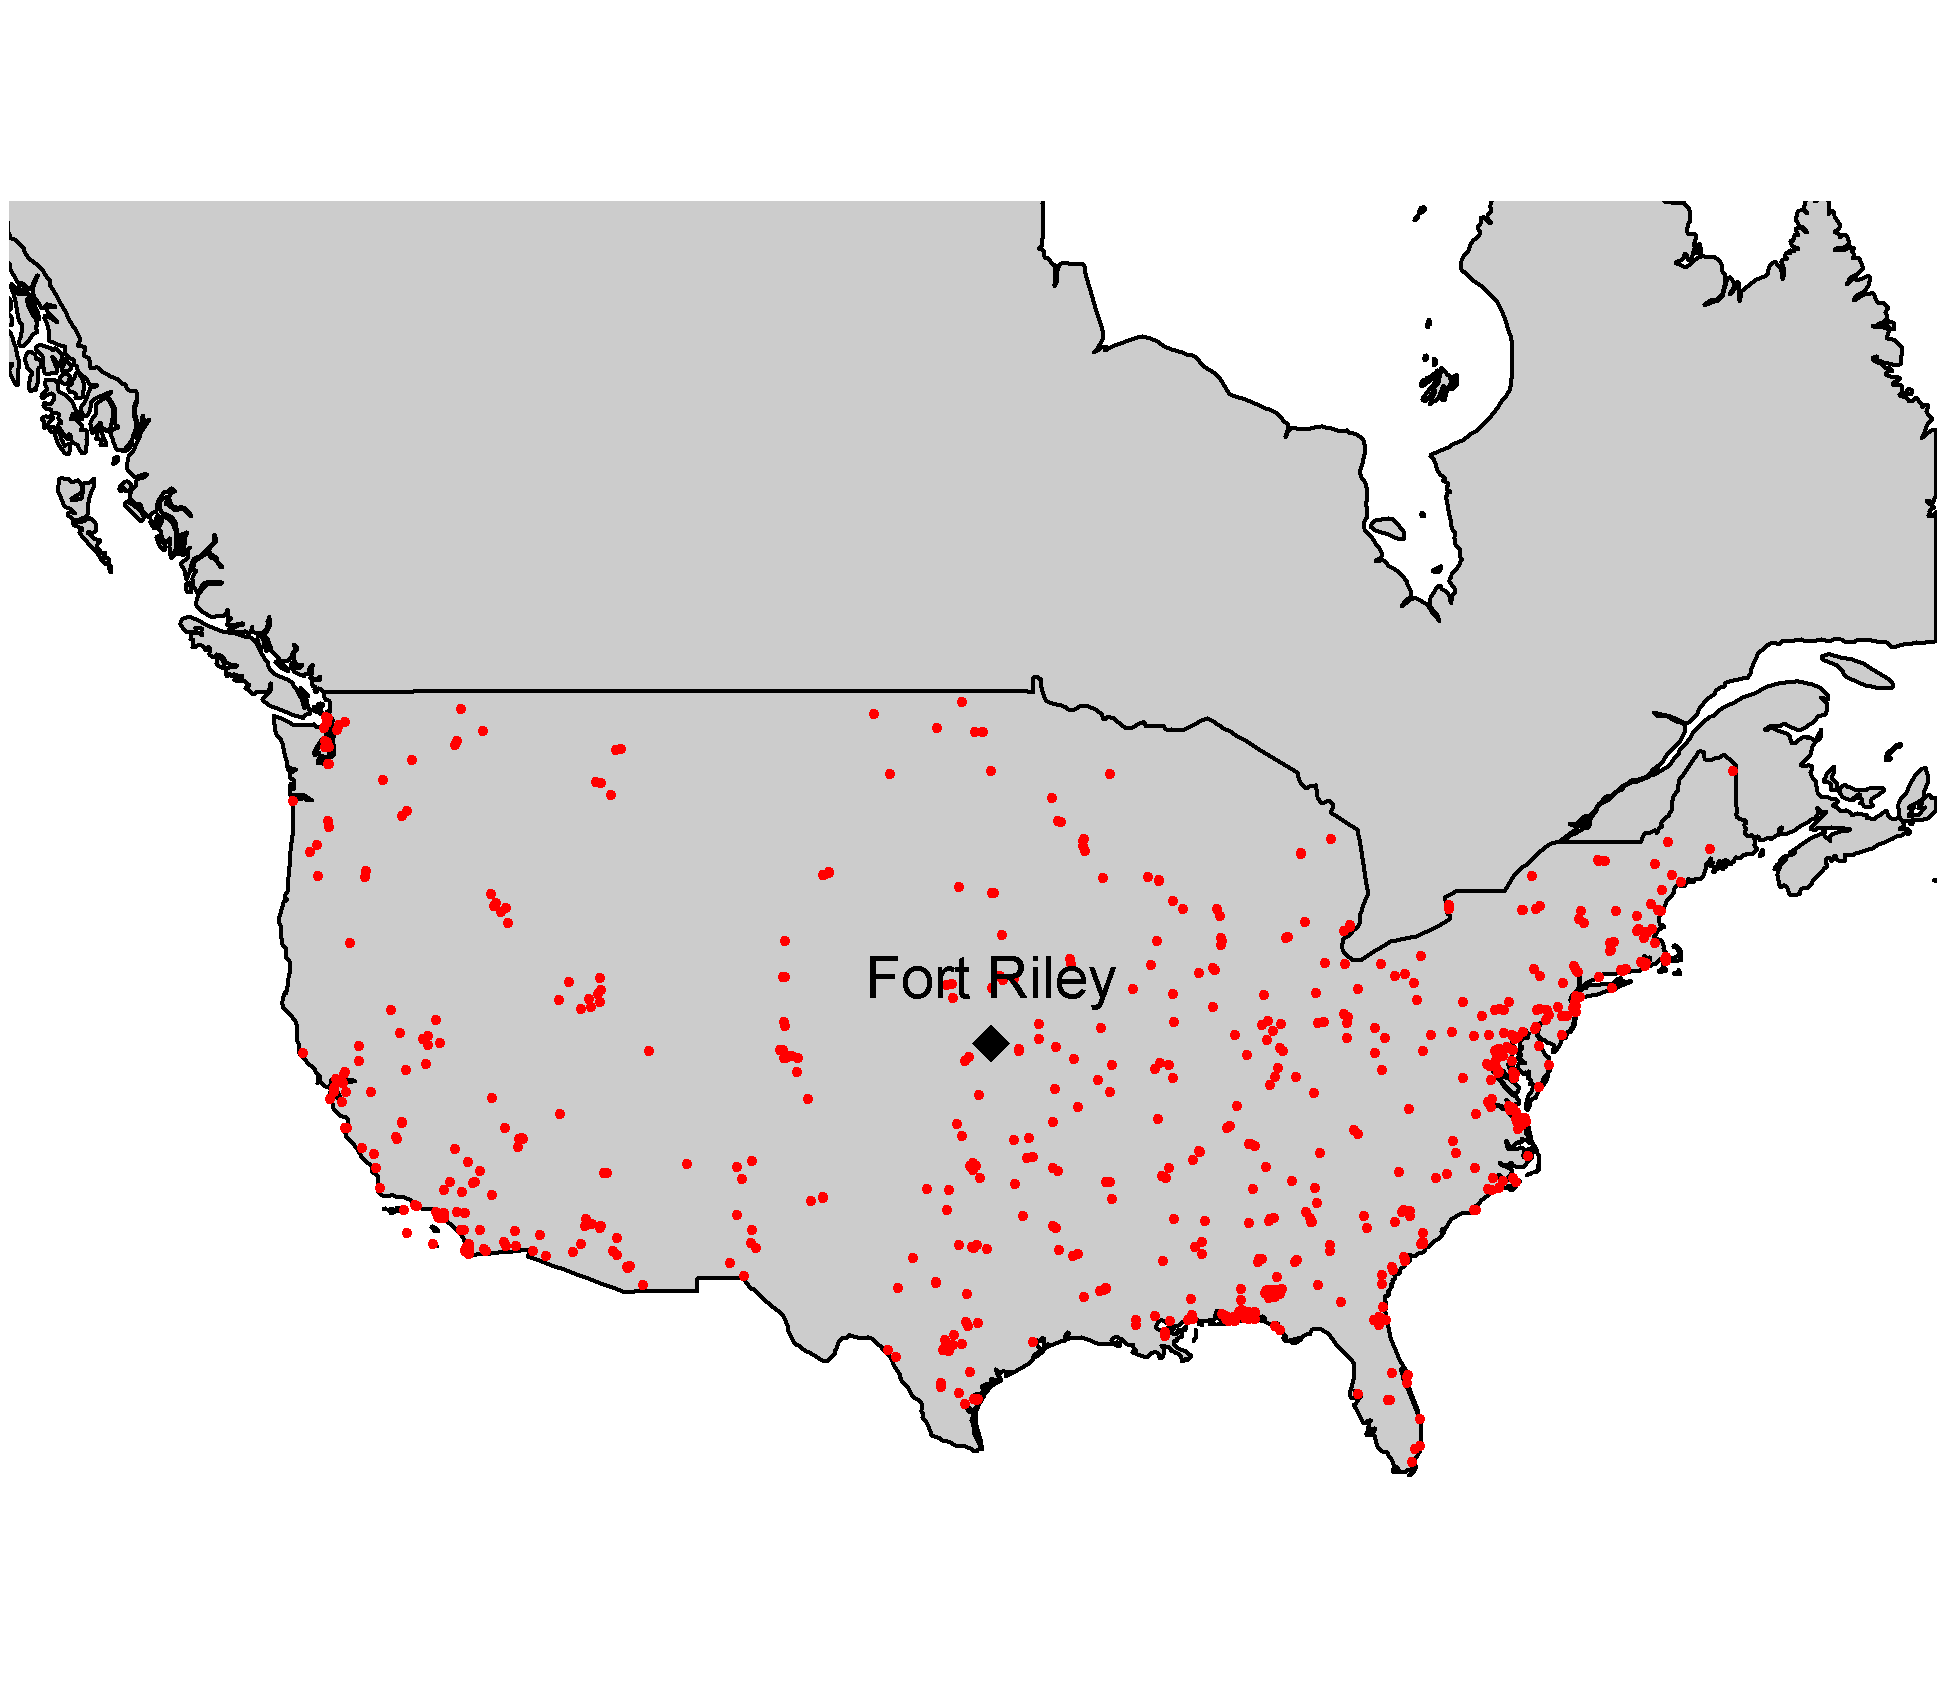
\includegraphics[width=0.85\linewidth]{./chapterFiles/fisherSpatial/figures/figsCalledInDiss/basesOfInterestMap} 

}

\caption{Locations of focal U.S. military bases, Eglin Air Force Base (AFB) and Fort Riley Military Base.}\label{fig:basesOfInterestMap}
\end{figure}
\hypertarget{spatial-sampling-grid}{%
\subsubsection{Spatial sampling grid}\label{spatial-sampling-grid}}

To my knowledge, Sundstrom et al. (2017) is the only study to use the Fisher Information on spatially-referenced data. The authors of this study hand-picked NABBS routes to be included in their samples such that their metrics should detect `regime changes' when adjacent sampling points represented different ecoregions (broad-scale vegetation classification system). The authors also suggest each ecoregion is similarly represented, having a similar number of NABBS routes within each ecoregion in the analysis. However, this method of handpicking routes resulted in a transect which was neither North-South nor East-West running (see Sundstrom et al. (2017)), but rather zigzagged across a midwestern region.
\begin{figure}
\includegraphics[width=0.85\linewidth]{./chapterFiles/fisherSpatial/figures/figsCalledInDiss/transectSamplingALlRoutesUsed} \caption{The three East-West running transects used to visualize results in this chapter.}\label{fig:ewRoutesUsedHere}
\end{figure}
I constructed a gridded system across the continental United States and parts of Canada. The gridded system comprises East-West running transects transects running in either North-South or East-West directions. This method ameliorates some sampling bias, as I have arbitrarily defined sampling transects, rather than hand-picking sites to include in the analysis. Additionally, this approach allows for raster stacking, or layering data layers (e.g., vegetation, LIDAR, weather) on top of the sampling grid and results, allowing one to identify potential relationships with large-scale drivers. This method also provides a simple vector for visualizing changes in the Fisher Information over space-time, using animations and still figures. For brevity, I present visual results of only three, spatially-adjacent, East-West running transects (Fig. \ref{fig:ewRoutesUsedHere}) at multiple time periods.

\hypertarget{calculating-fisher-information-fi}{%
\subsection{Calculating Fisher Information (FI)}\label{calculating-fisher-information-fi}}

Fisher Information, \(I(\theta)\), was developed in 1922 by Ronald Fisher as a measure of the amount of information that an observable variable, X, reveals about an unknown parameter, \(\theta\). Fisher Information is a measure of indeterminacy (Fisher 1922) and is defined as,
\begin{equation} 
  I(\theta) = \int \frac{dy}{p(y|\theta)}\left[\frac{dp(y|\theta)}{d\theta}\right]^2
  \label{eq:fiGeneral1922}
\end{equation}
where \(p(y|\theta)\) is the probability density of obtaining the data in presence of \(\theta\). The Fisher Information measure (FIM) is used to calculate the covariance matrix associated with the likelihood, \(p(y|\theta)\). Fisher Information is described as Extreme Physical Information (EPI; Frieden and Soffer 1995, Kibble 1999, Frieden et al.~2002), a measure that has been used to track the complexity of systems in many scientific disciplines including, physics, cancer research, electrical engineering, and, recently, complex systems theory and ecology

Fisher Information as gathered from observational data provides insight as to the dynamic order of a system, where an orderly system is one with constant (i.e., unchanging) observation points, and one whose nature is highly predictable. A disorderly system is just the opposite, where each next data point is statistically unpredictable. In ecological systems, patterns are assumed to be a realization of ecosystem order; therefore, oneshould expect orderliness in a system with relatively stable processes and feedbacks. Orderliness, however, does not necessarily infer long-term predictability. Equation \eqref{eq:fiGeneral1922} is next adapted to estimate the dynamic order of an entire system, \(s\), as
\begin{equation} 
  I = \int \frac{ds}{p(s)}\left[\frac{dp(s)}{ds}\right]^2
  \label{eq:fi73c}
\end{equation}
where \(p(s)\) is the probability density for \(s\). Here, a relatively high Fisher Information value (\(I\)) infers higher dynamic order, whereas a lower value (approaching zero) infers less orderliness. To limit the potential values of \(I\) in real data, we can calculate the amount of Fisher Information by re-expressing it in terms of a probability amplitude function \(q(s)\) (Fath et al.~2003, Mayer et al.~2007, eq. 7.3):
\begin{equation}
  I = 4 \int ds\left[\frac{dq(s)}{ds}\right]^2
  \label{eq:fiAmp}
\end{equation}
A form specific to the pdf of distance travelled by the entire system, which I call the `derivatives' method, is defined as (Mayer et al., 2007, eq. 7.12):
\begin{equation}
  I = \frac{1}{T} \int_0^T dt\left[\frac{s''^2}{s'^4}\right]^2
  \label{eq:fiDerivs}
\end{equation}
where T is the number of equally spaced time points over which the data are integrated. Numerical calculation of \(I\) using the binning method (Eq. \eqref{eq:fiAmp} and \eqref{eq:fiDerivs}) each incorporate a moving-window procedure for calculating the probability of the system, \(p(s)\), as being in one of an unidentified number of states (\(s\)). Although previously applied to spatially-explicit terrestrial community data,the binning method (Eq. \ref{derivatives}) requires multiple parameters to be defined \emph{a priori}, which have been shown to influence inference based on the metric. I therefore calculated FI using the derivatives equation (Eq. \ref{fiDerivs}).

The binning procedure allows for a single point in time or space to be categorized into more than one state, which violating the properties of alternative stable states theory. The size of states (see Eason and Cabezas 2012) measure is required to construct p(s). In the case of high dimensional data, a univariate binning procedure of p(s) is not intuitive (i.e., reducing a multivariable system to a single probability distribution rather than constructing a multivariate probability distribution). Importantly, when using community or abundance data, rare or highly abundant species can influence the size of states criterion, thus influencing the assignment of each point into states. Finally, Eq. \eqref{eq:fiAmp} assumes equal spacing (in space or time) between sampling points. Each of these violations can be avoided by using Eq. \eqref{eq:fiDerivs}; Cabezas and Fath 2002, Fath et al.~2003) to calculate the Fisher Information measure. The derivatives method (Eq. \eqref{eq:fiDerivs}) estimates the trajectory of the system's state by calculating the integral of the ratio of the system's acceleration and speed in state space (Fath et al., 2003). I calculated Fisher Information using Equation \eqref{eq:fiDerivs} for all East-West transects (see Fig. \ref{fig:ewRoutesUsedHere}) for years 1980, 1990, 2000, and 2010.

\hypertarget{interpreting-and-comparing-fisher-information-across-spatial-transects}{%
\subsection{Interpreting and comparing Fisher Information across spatial transects}\label{interpreting-and-comparing-fisher-information-across-spatial-transects}}

\hypertarget{interpreting-fisher-information-values}{%
\subsubsection{Interpreting Fisher Information values}\label{interpreting-fisher-information-values}}

Here I define a potential regime change as a point(s) having a non-zero derivative, and at which relatively large changes (sharp increase or decrease) in the Fisher Information measure occur. Regime shifts are identified as data changing from one state to another, thus, rapid shifts in the value of FI should indicate the points, in time or space, at which the system undergoes reorganization. Spatial and temporal Fisher Information calculation does not vary, but interpretation of either differ in that a spatial analysis will identify a spatial regime boundary (Sundstrom et al., 2017) in space within a single time period, whereas analysis of temporal data will identify a point(s) in time at which a system in a specific location undergoes a regime shift. I follow the methods outlined in the relevant literature for interpreting the Fisher Information (e.g., Karunanithi et al., 2008, p. @eason\_evaluating\_2012).

Increases in FI is proposed as an indicator of system orderliness, where periods of relatively high values of FI indicate the system is in an ``orderly'' state, or is fluctuating around a single attractor. A rapid change in FI is supposed to indicated the system is no longer orderly and may be undergoing a reorganization phase. Whether Fisher Information can identify a switch among basins of attraction within a single, stable state (or around a single attractor) remains unknown, as does the number of states which a system can occupy. When a system occurs within any number of states equally, i.e., p(s) is equal for each state, both the derivative, (\(\frac{dq(s)}{ds}\), and \(I\) are zero. As \((\frac{dq(s)}{ds} \rightarrow \infty)\), we infer the system is approaching a stable state, and as \(\frac{dq(s)}{ds} \rightarrow 0\) the system is showing no preference for a single stable state and is on an unpredictable trajectory. \eqref{eq:fiAmp} bounds the potential values of Fisher Information at \([0, 8]\), whereas \eqref{eq:fiGeneral1922}, \eqref{eq:fi73c}, and \eqref{eq:fiDerivs} are positively unbounded \([0, \infty)\). If the Fisher Information is assumed to represent the probability of the system being observed in some state, \(s\), then the absolute value of the Fisher Information index is relative within a single datum (here, transect). It follows that Fisher Information should be interpreted relatively, but not absolutely.

\hypertarget{interpolating-results-across-spatial-transects}{%
\subsubsection{Interpolating results across spatial transects}\label{interpolating-results-across-spatial-transects}}

Because the BBS routes are not regularly spaced, pairwise correlations of adjacent transects are not possible without either binning the Fisher Information calculations using a moving-window analysis, or interpolating the results to regularly-spaced positions in space. To avoid potential biases associated with the former option, I linearally interpolated Fisher Information within each spatial transect (Fig. \ref{fig:ewRoutesUsedHere}) at 50 points along the longitudinal axis. The 50 longitudinal points at which I interpolated were the same across each spatial transect. I used the function \emph{stats::approx()} to linearly approximate the Fisher Information. I did not interpolate values beyond the longitudinal range of the original data (using argument \emph{rule=1} in package \emph{approx}).
\begin{figure}
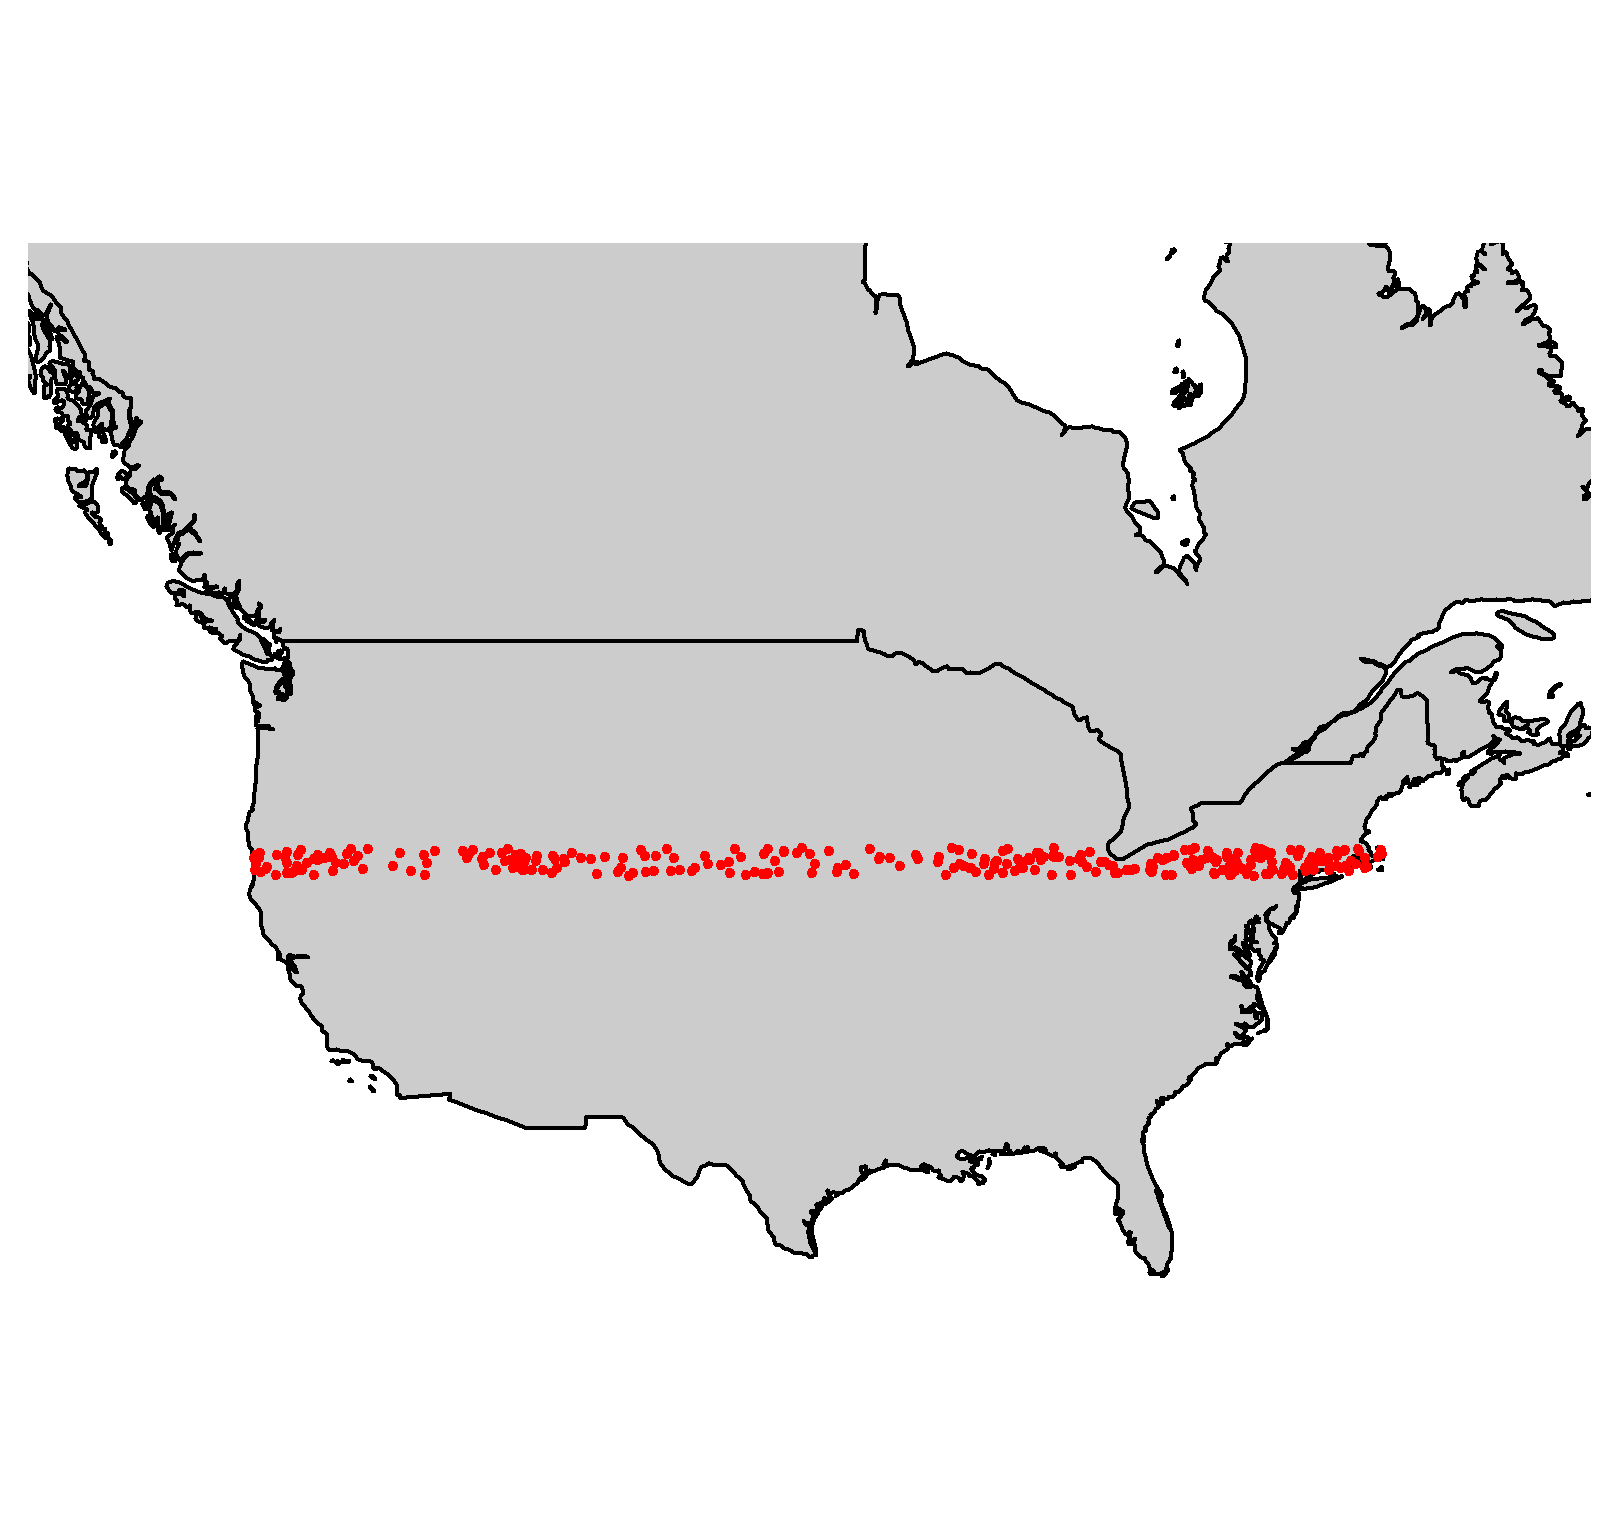
\includegraphics[width=0.85\linewidth]{./chapterFiles/fisherSpatial/figures/figsCalledInDiss/transectSamplingEx_1row} \caption{An example of two adjacent spatial transects within my sampling grid.}\label{fig:oneTsectEx}
\end{figure}
\begin{figure}
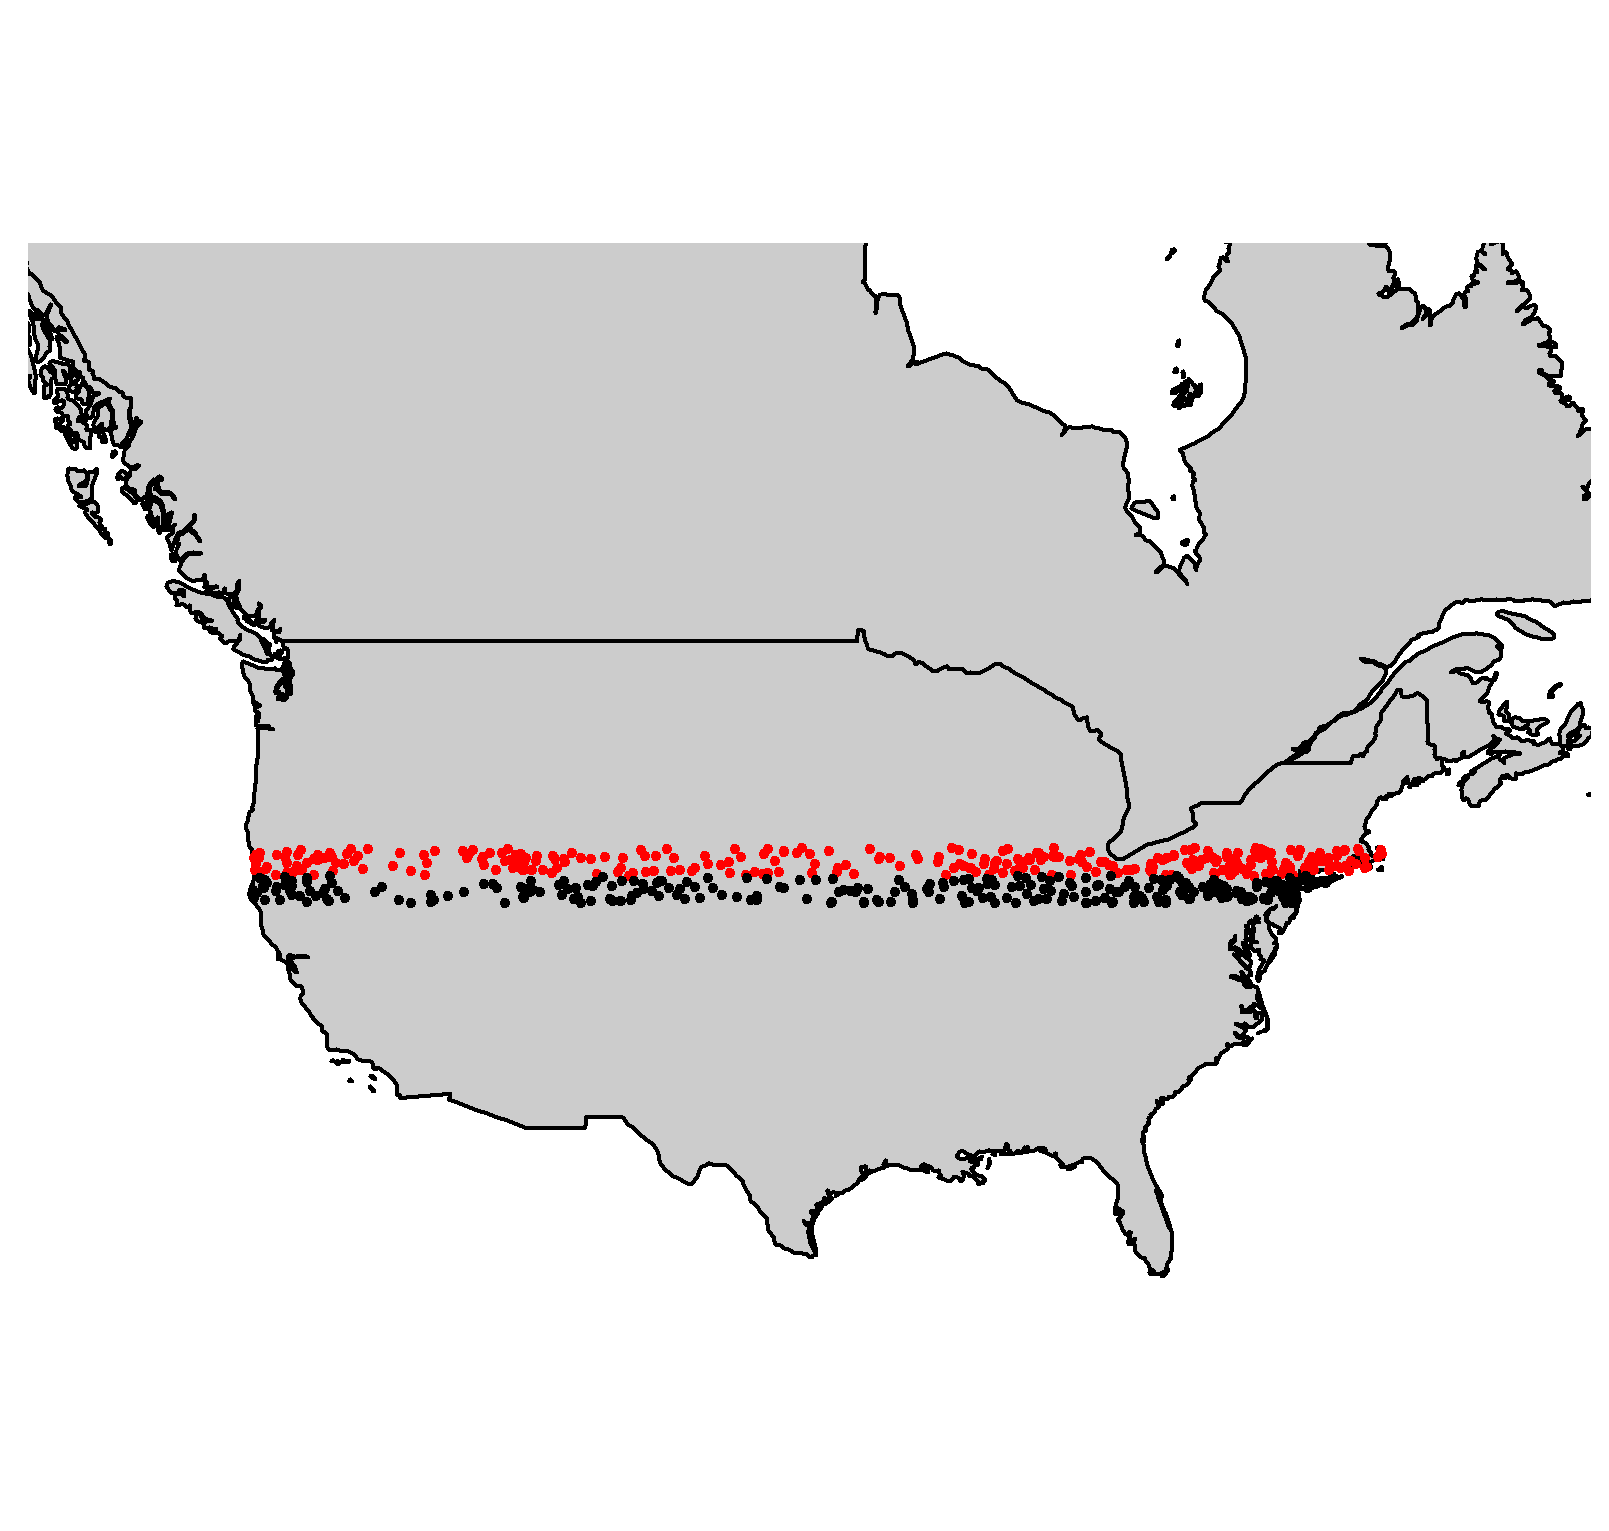
\includegraphics[width=0.85\linewidth]{./chapterFiles/fisherSpatial/figures/figsCalledInDiss/transectSamplingEx_2rows} \caption{An example of two adjacent spatial transects (12, 13) within my sampling grid.}\label{fig:adjacentTsectEx}
\end{figure}
\hypertarget{spatial-correlation-of-fisher-information}{%
\subsubsection{Spatial correlation of Fisher Information}\label{spatial-correlation-of-fisher-information}}

If Fisher Information captures and reduces information regarding abrupt changes in community structure across the landscape, then the values of FI should be spatially autocorrelated. That is, the correlation of FI values should increase as the distance between points decreases. Fisher Information values calculated using Eq. \eqref{eq:fiDerivs} are \textbf{not} relatively comparable outside of our spatial transects, because the possible values are unbounded (can take on any value between \(-\infty\) and \(\infty\). However, because FI is directly comparabe \textbf{within} each spatial transect (e.g., \ref{fig:oneTsectEx}), we can use use pairwise correlations among two transects (e.g., \ref{fig:oneTsectEx}) to determine whether values of FI are consistent across space. I calculate the pairwise correlation (Pearson's) among each pair of adjacent spatial transects (e.g., Fig. \ref{fig:adjacentTsectEx}). I removed a pair of points if at least one point was missing an estimate for Fisher Information. This occurred when the original longitudinal range of one transect exceeded its pair's range, since I did not interpolate beyond the original longitudinal range.

\hypertarget{results-1}{%
\section{Results}\label{results-1}}

\hypertarget{fisher-information-across-spatial-transects}{%
\subsection{Fisher Information across spatial transects}\label{fisher-information-across-spatial-transects}}
\begin{figure}
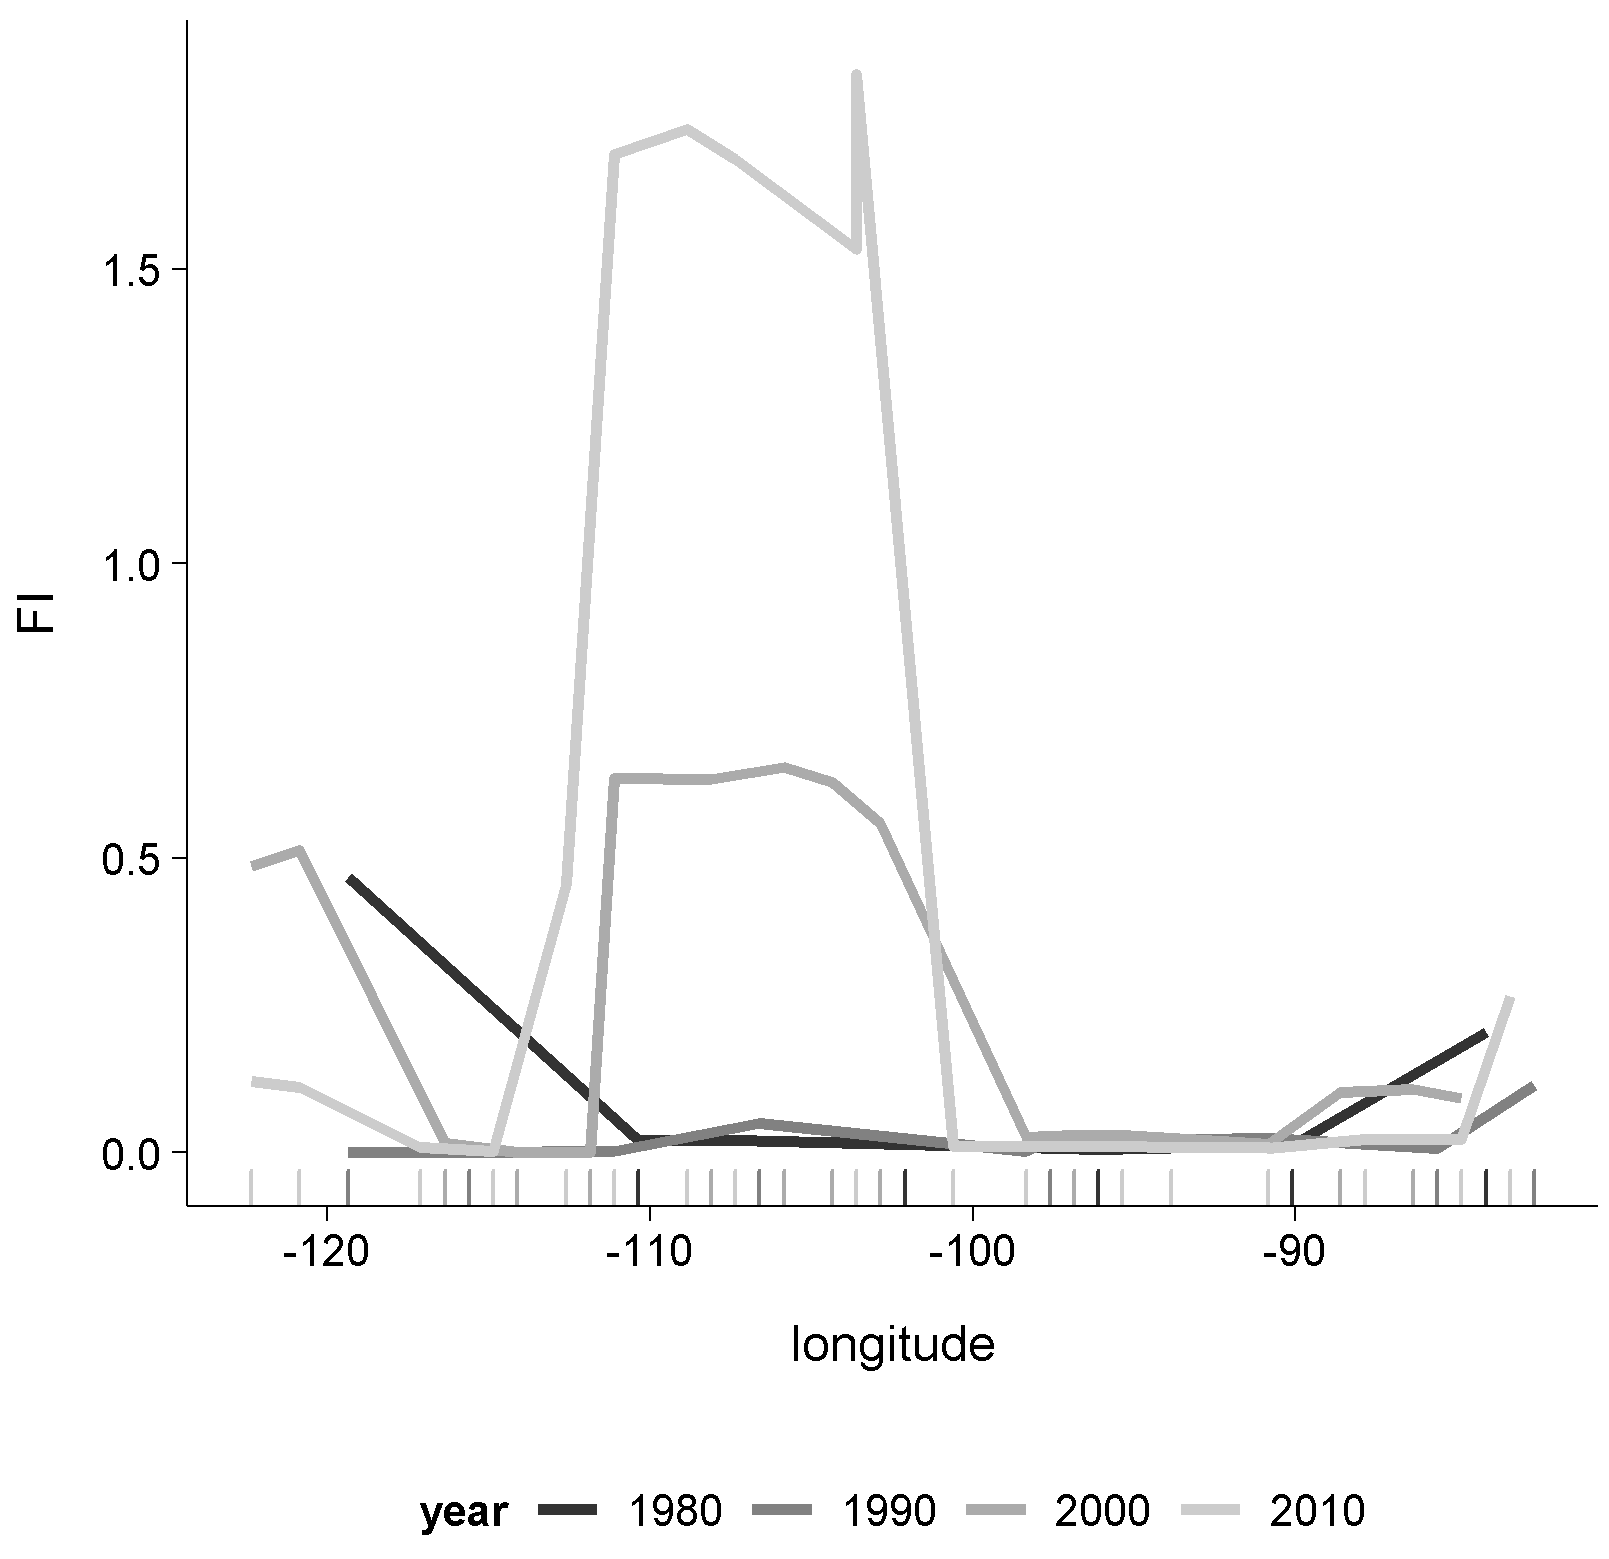
\includegraphics[width=0.85\linewidth]{./chapterFiles/fisherSpatial/figures/figsCalledInDiss/transect_12_East-West_metric_FI_Eqn7_12} \caption{Fisher Information calculated for a single transect over time.}\label{fig:fi1Tsect}
\end{figure}
Interpreting the Fisher Information is currently a qualitative effort. As suggested earlier, rapid increases or decreases in FI are posited indicate a change in system orderliness, potentially suggesting the location of a regime shift. Using this method yields inconclusive results regarding the location of `spatial regimes' (Fig. \ref{fig:fi1Tsect}). Of the three spatial transects analyzed in this chapter (Fig. \ref{fig:ewRoutesUsedHere}), Fig.\ref{fig:fi1Tsect} is representative of the lack of pattern observed in the Fisher Information values aross transects. I identified no clear pattern within or among spatial transects. Log-transforming the Fisher Information metric suppresses some of the extreme values, but still does not clearly identify sharp changes in the Fisher Information values.
\begin{figure}
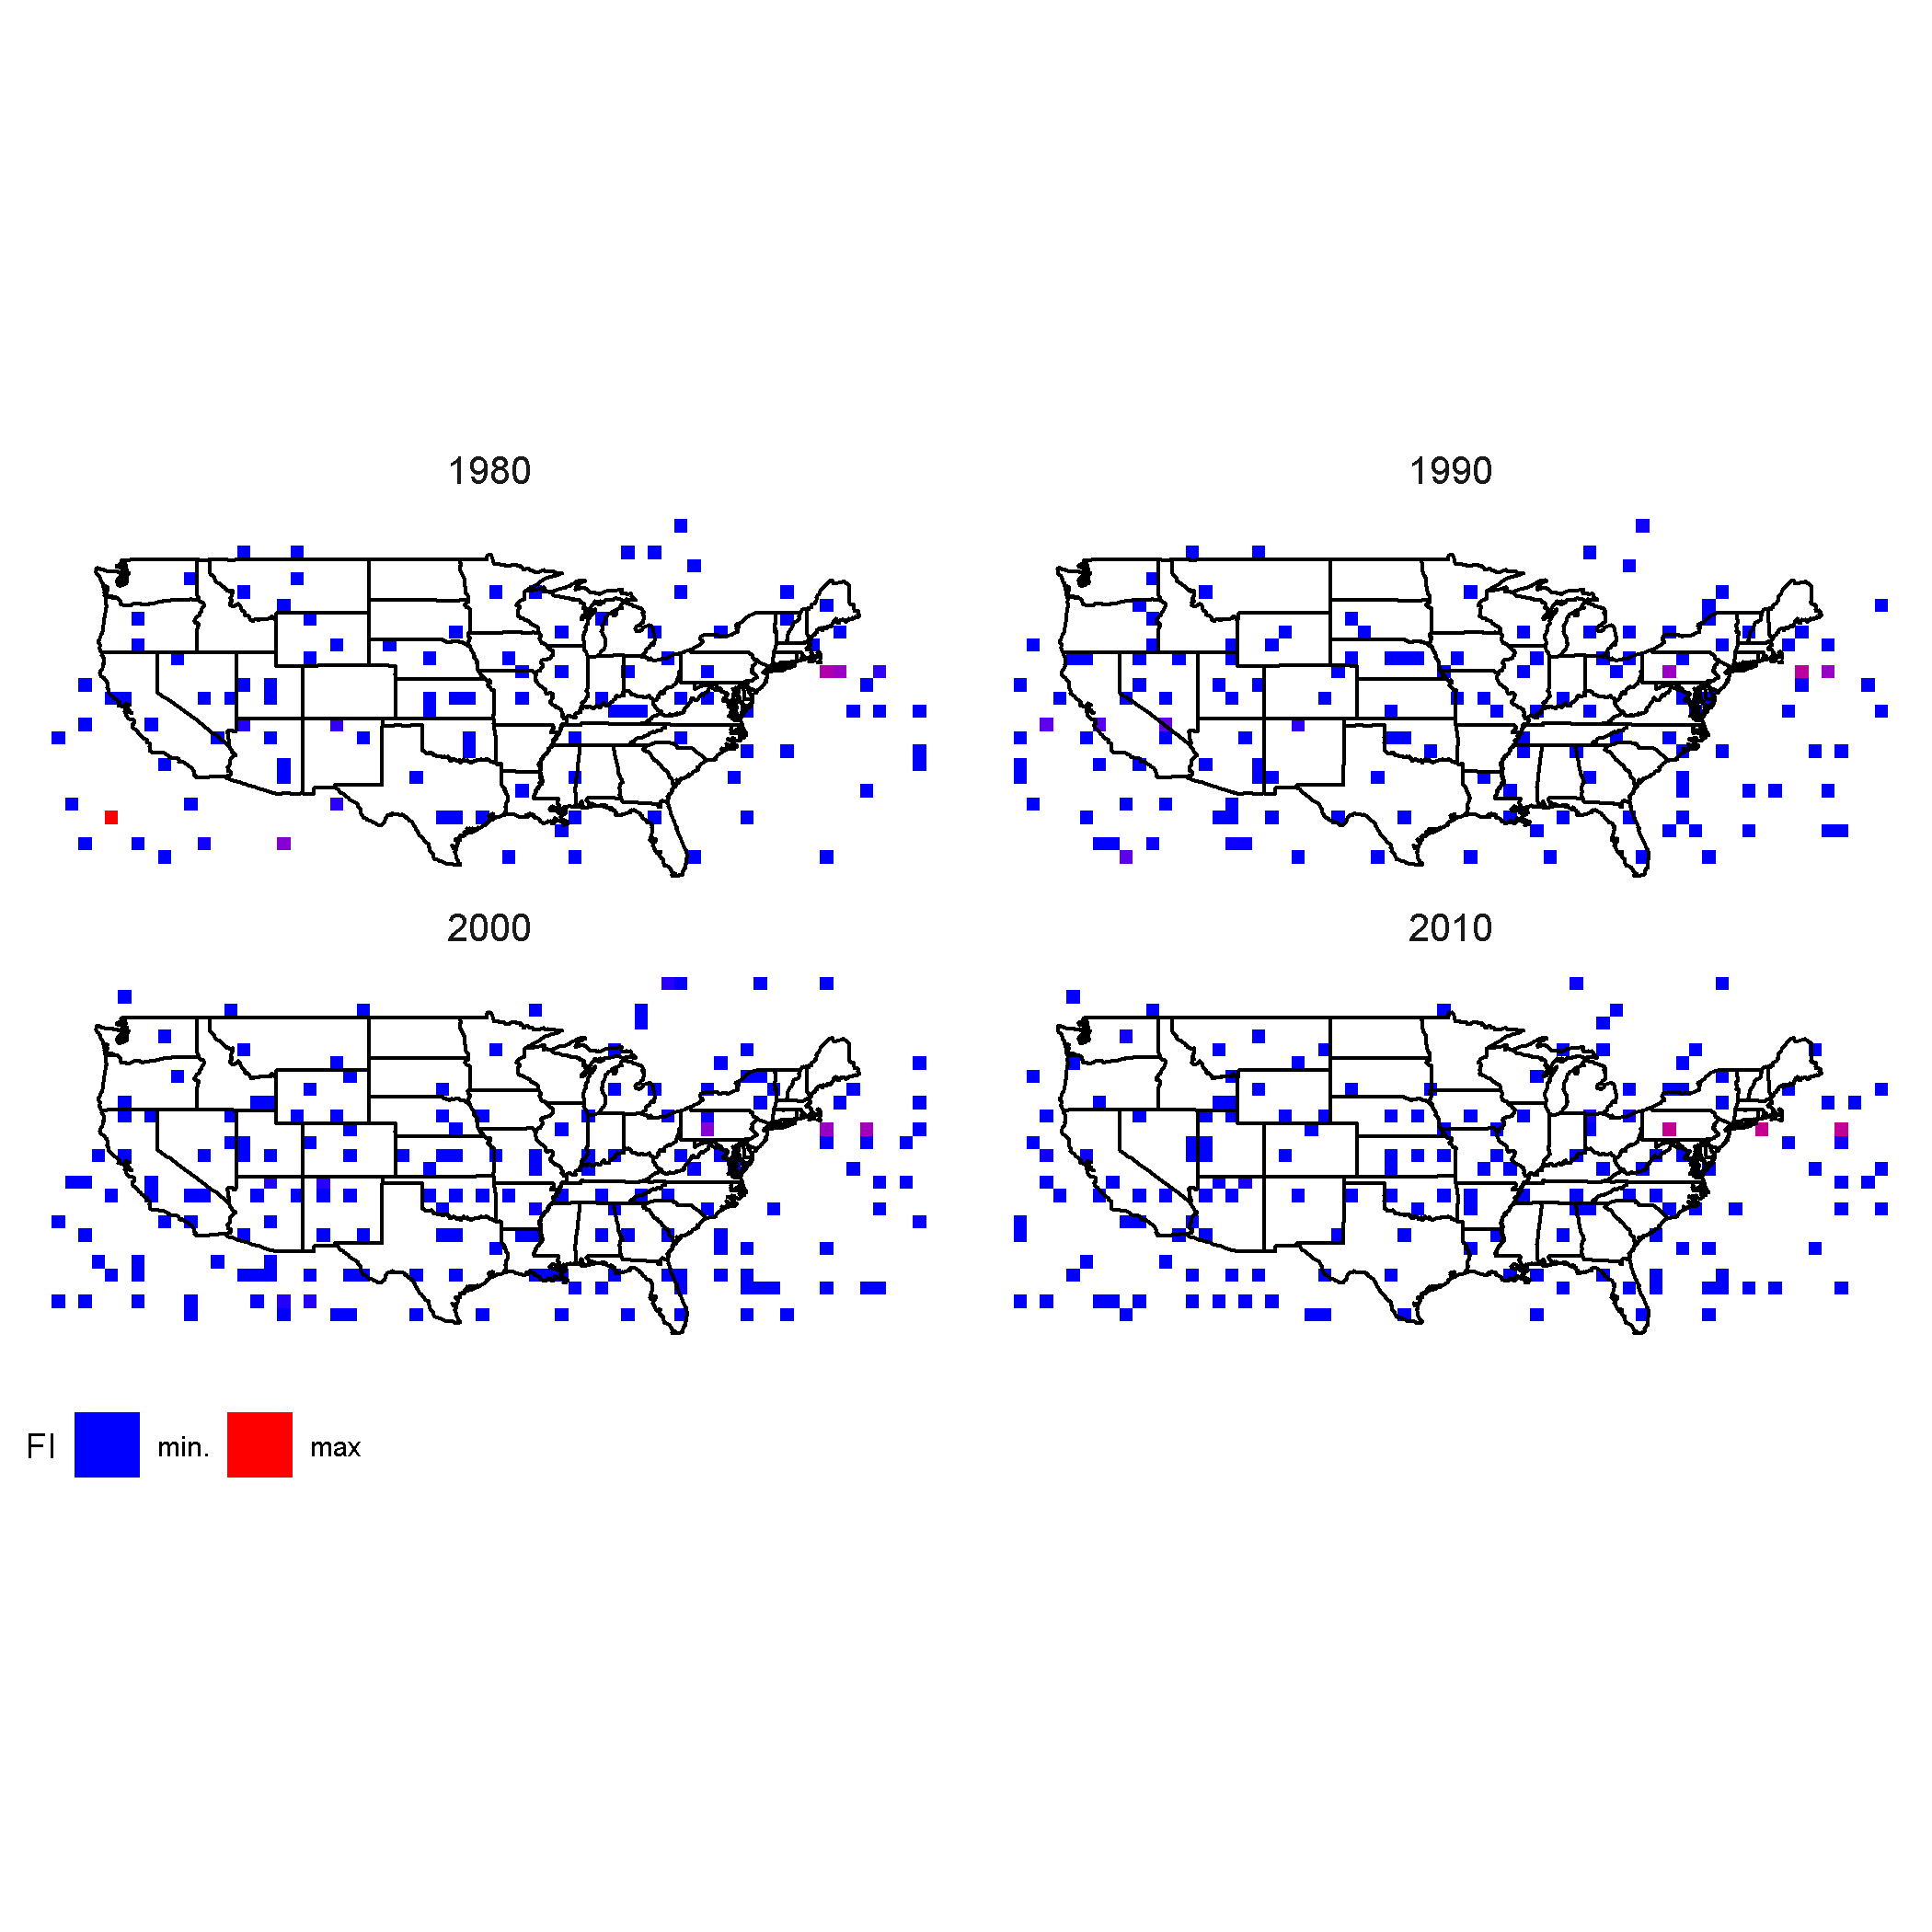
\includegraphics[width=0.85\linewidth]{./chapterFiles/fisherSpatial/figures/figsCalledInDiss/usaAllTsects_East-West_metric_FI} \caption{Fisher Information of 5 East-West spatial transects over time.}\label{fig:usaFI}
\end{figure}
\begin{figure}
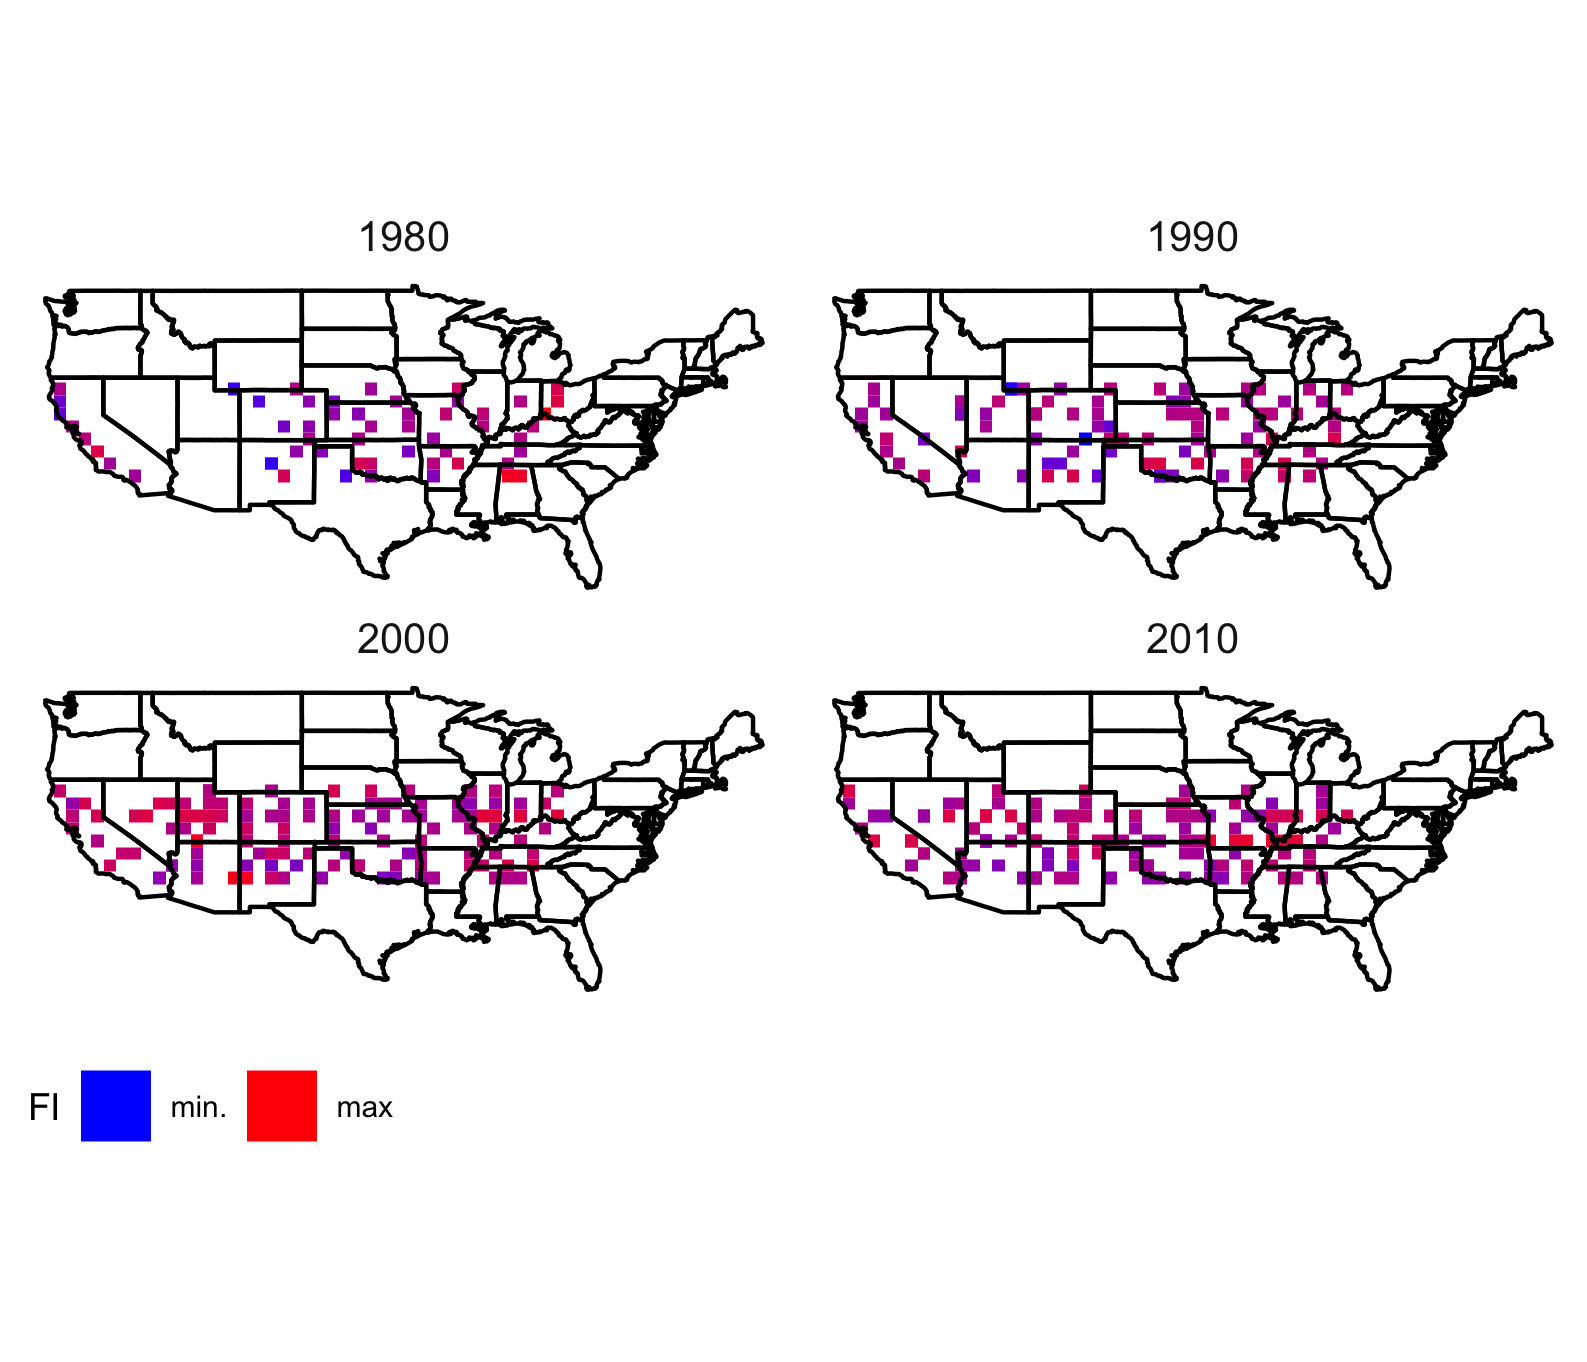
\includegraphics[width=0.85\linewidth]{./chapterFiles/fisherSpatial/figures/figsCalledInDiss/usaAllTsects_East-West_metric_logScaleFI} \caption{Fisher Information of 5 East-West spatial transects over time.}\label{fig:usaFI}
\end{figure}
\begin{figure}
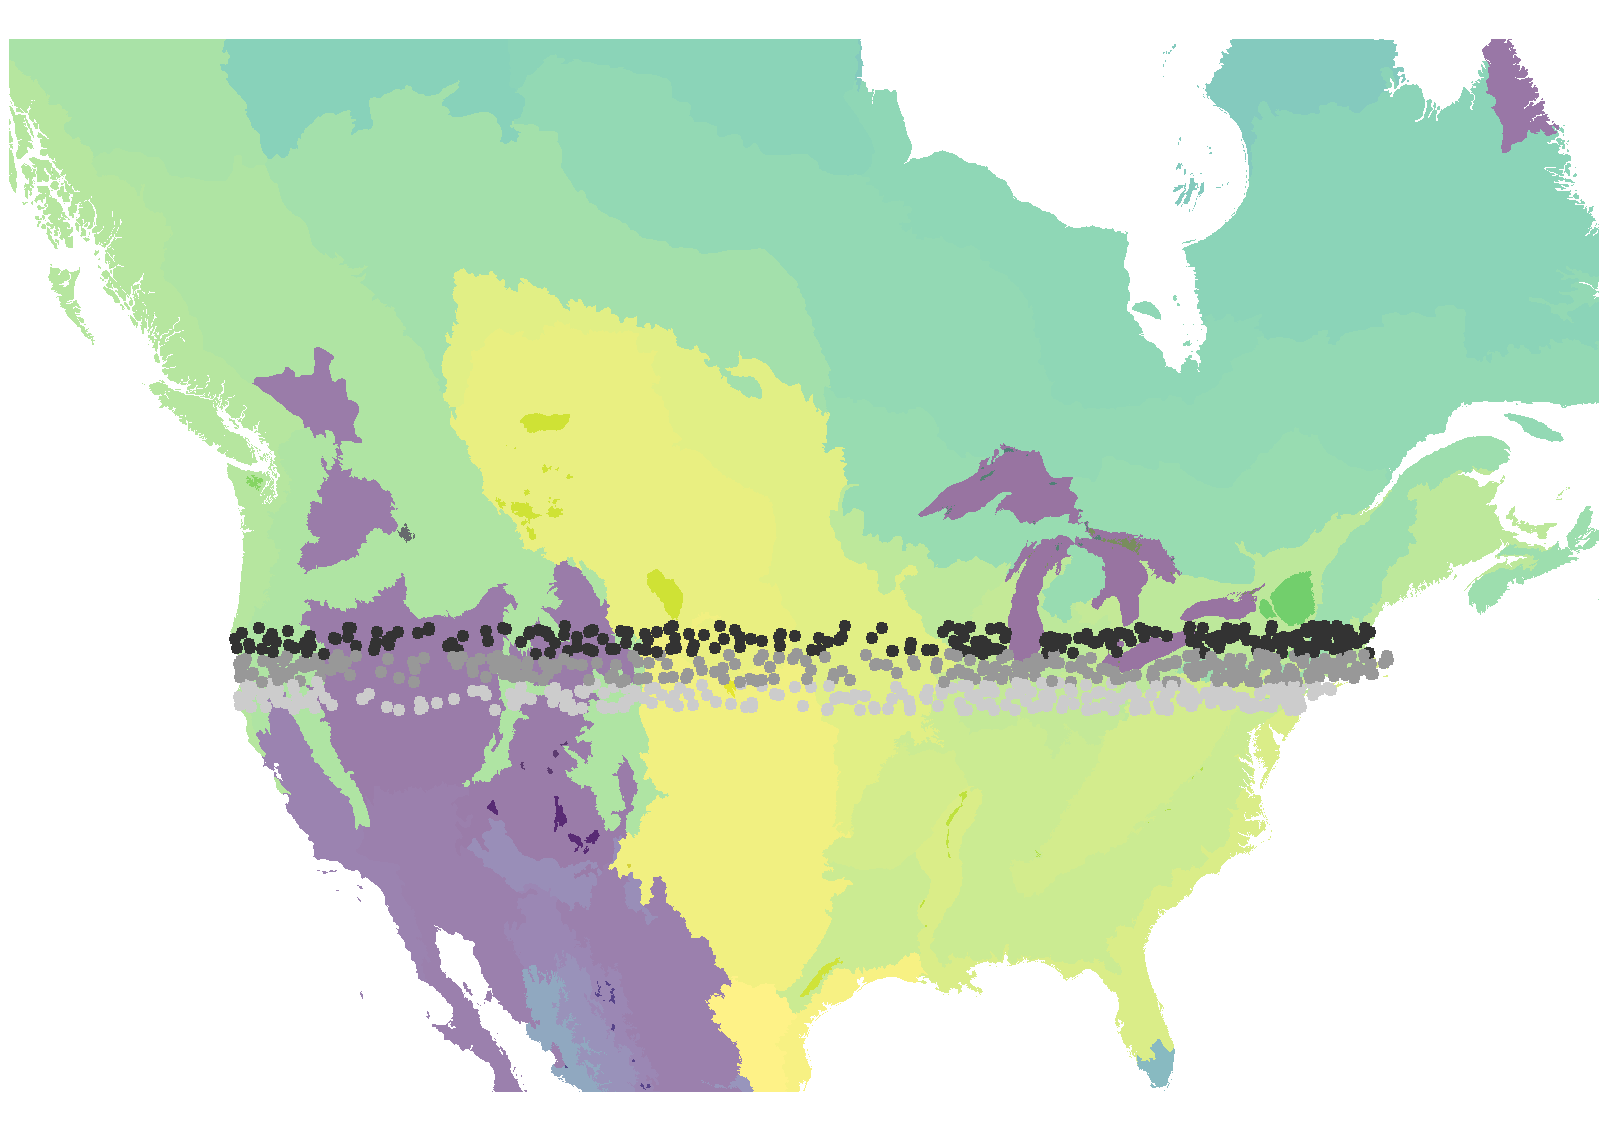
\includegraphics[width=0.85\linewidth]{./chapterFiles/fisherSpatial/figures/figsCalledInDiss/allRoutesUsed_ecoregions} \end{figure}
\begin{figure}
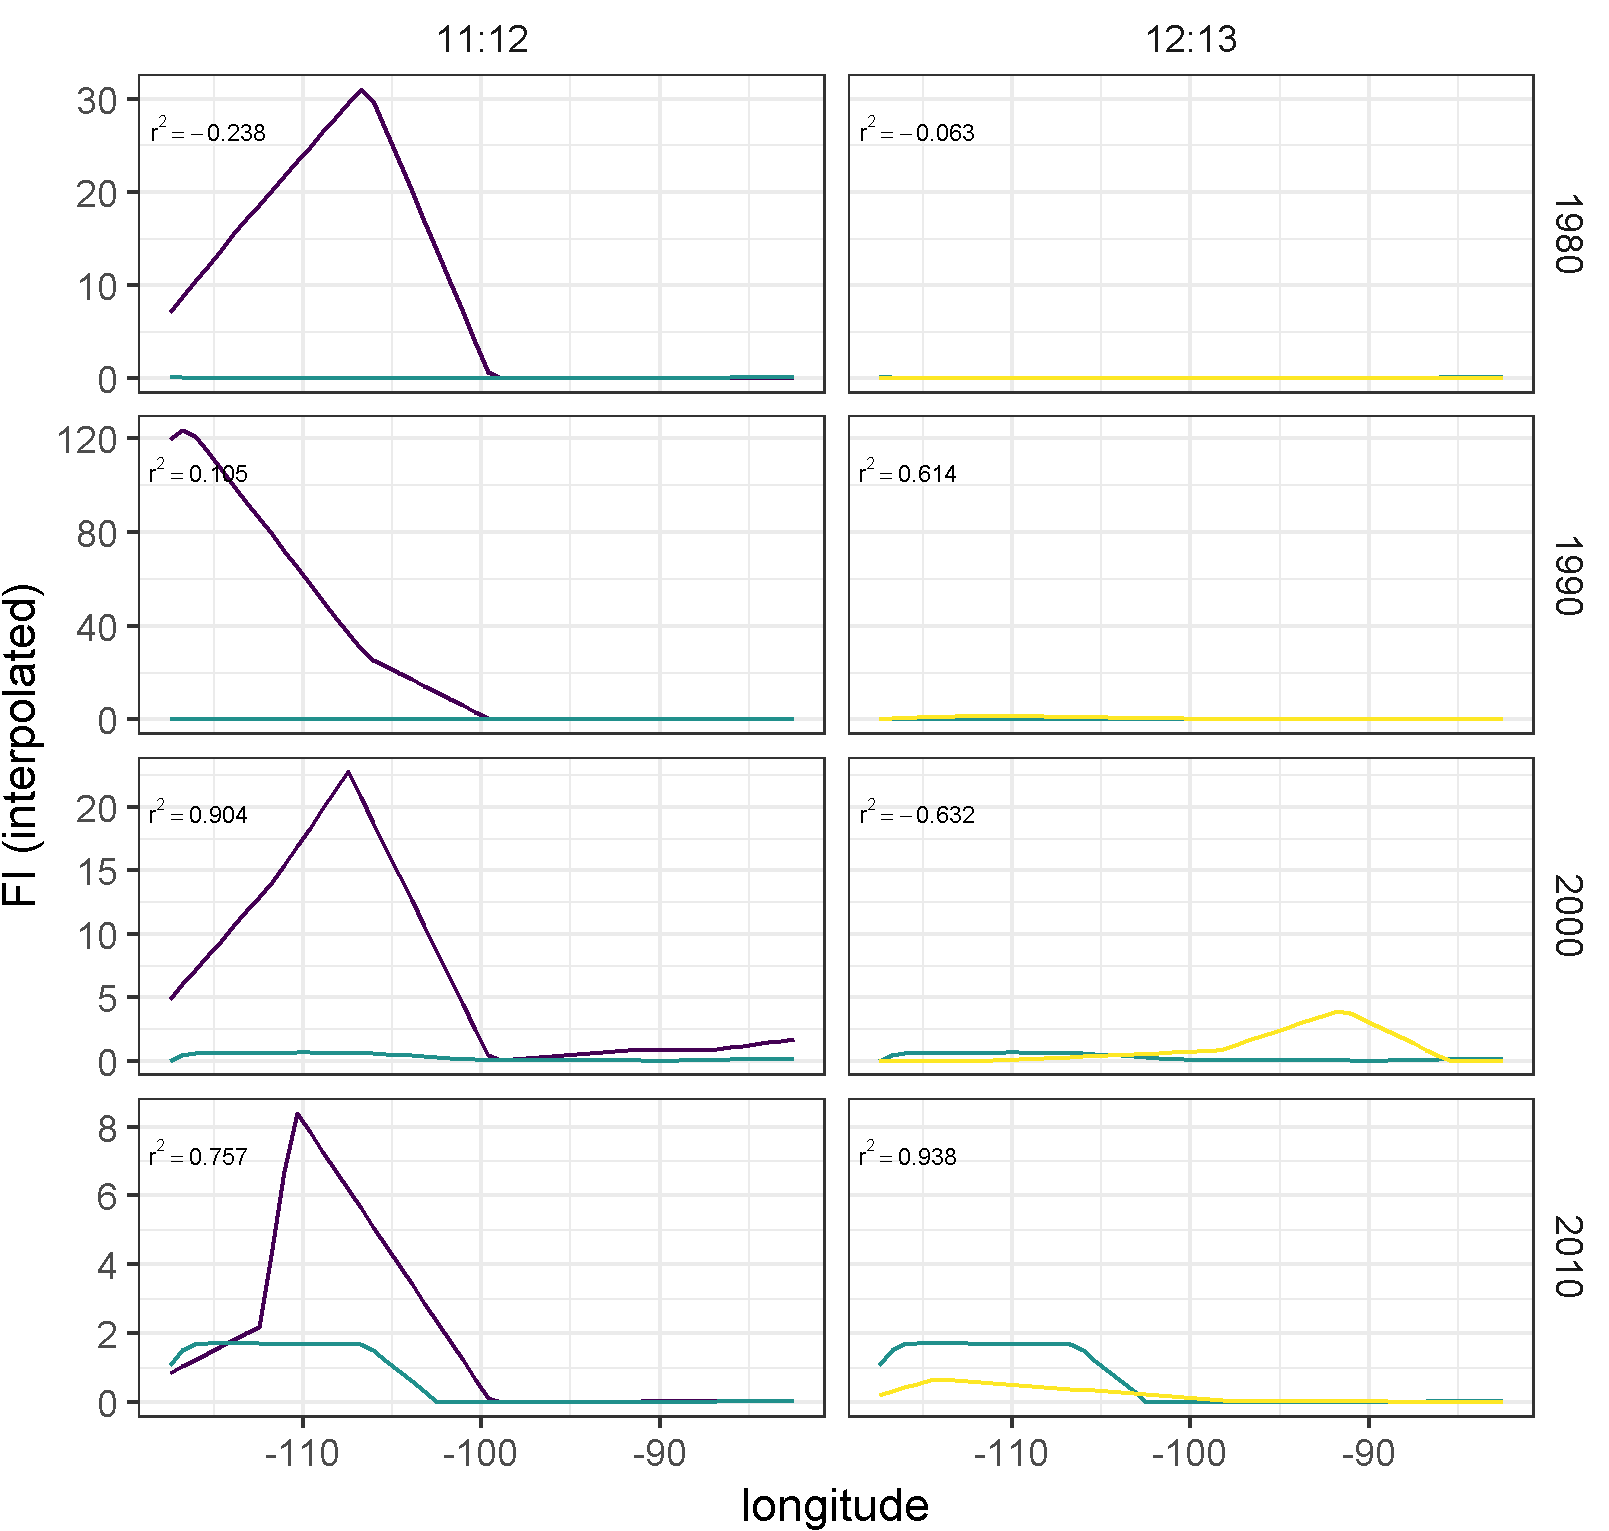
\includegraphics[width=0.85\linewidth]{./chapterFiles/fisherSpatial/figures/figsCalledInDiss/interpolated_FI_corplotSelectTransects_East-West} \caption{Pairwise relationships of Fisher Information (interpolated values) of spatially adjacent transects over time. }\label{fig:corPlotTsectsInterp}
\end{figure}
\begin{figure}
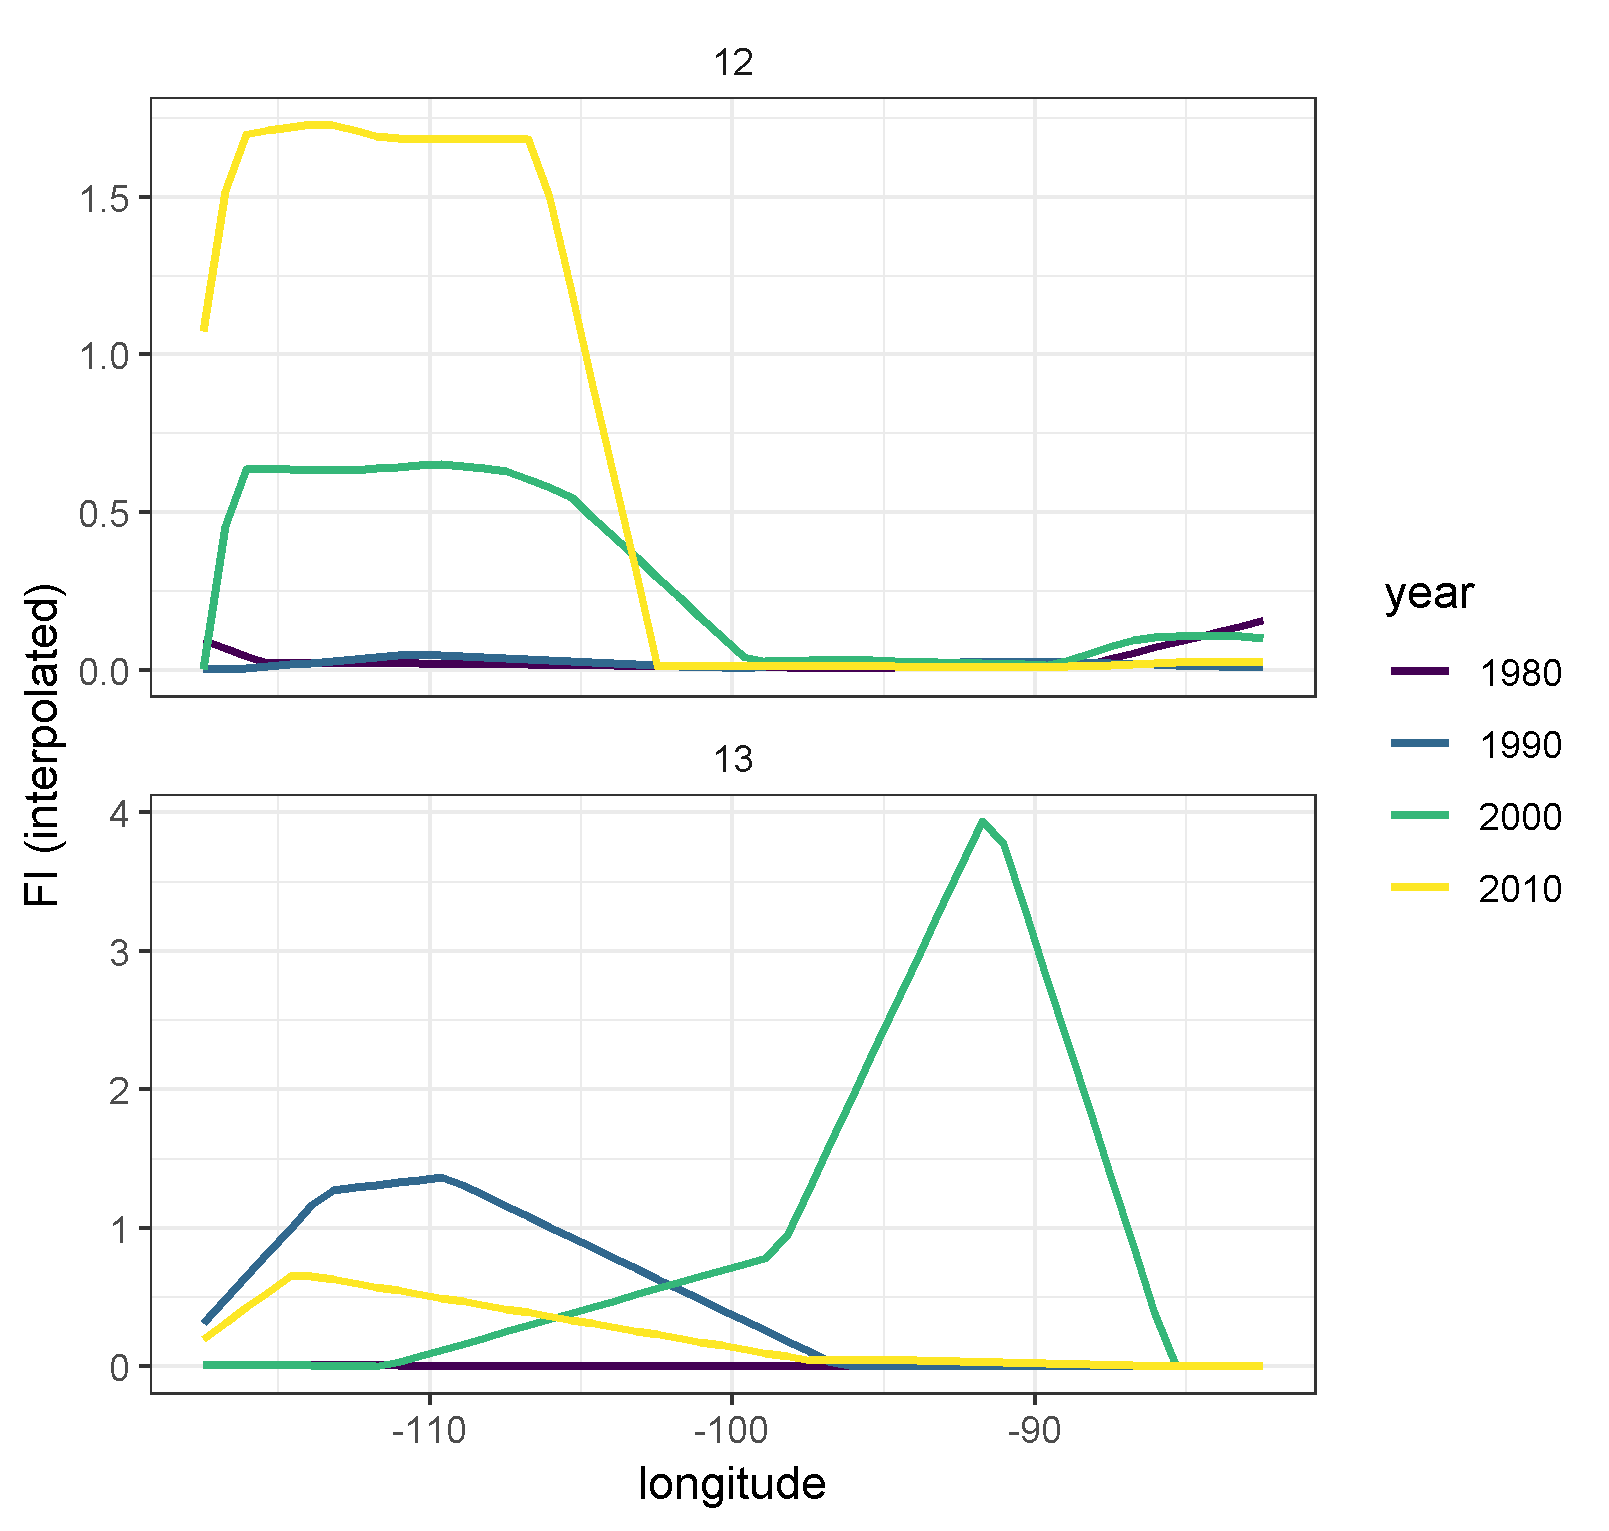
\includegraphics[width=0.85\linewidth]{./chapterFiles/fisherSpatial/figures/figsCalledInDiss/interp_FI_singlePair_corPlot_East-West} \caption{Fisher Information of two transect pairs over time. }\label{fig:fiSinglePair}
\end{figure}
\hypertarget{spatial-correlation-of-fisher-information-1}{%
\subsection{Spatial correlation of Fisher Information}\label{spatial-correlation-of-fisher-information-1}}

In addition to failing to identfiy clear geological boundaries across large swaths of our study area, (Fig \ref{fig:usaFI}) I also did not identify spatial correlation of Fisher Information among adjacent spatial transects (Fig. \ref{fig:corPlotTsectsInterp})\footnote{Pairs were compared (column) at select sampling years (rows), and pair-wise correlations among paired transects are presented. Large, positive correlations indicate Fisher Information signals similarly at adjacent spatial transects.}. For spatially-adjacent transects (e.g, transects 11 and 12, or 12 and 13 in Fig. \ref{fig:corPlotTsectsInterp}), we should expect high and positive correlation values, and these values shoudl stay consistent across time \emph{unless} the spatial transects were separated by an East-West running physical or functional boundary. This is not, however, what I expect in our East-West running transects (Fig. \ref{ewRoutesUsedHere}), as the spatial soft-boundaries limiting the distribution and functional potential of avian communities are largely North-South (Fig. @ref(ewRoutes\_ecoRegions)). Note spatial transects in Fig. @ref(fig:ewRoutes\_ecoRegions) overlap multiple, large spatial ecoregion boundaries, such that we should expect our data to identify these points (boundaries).
\begin{figure}
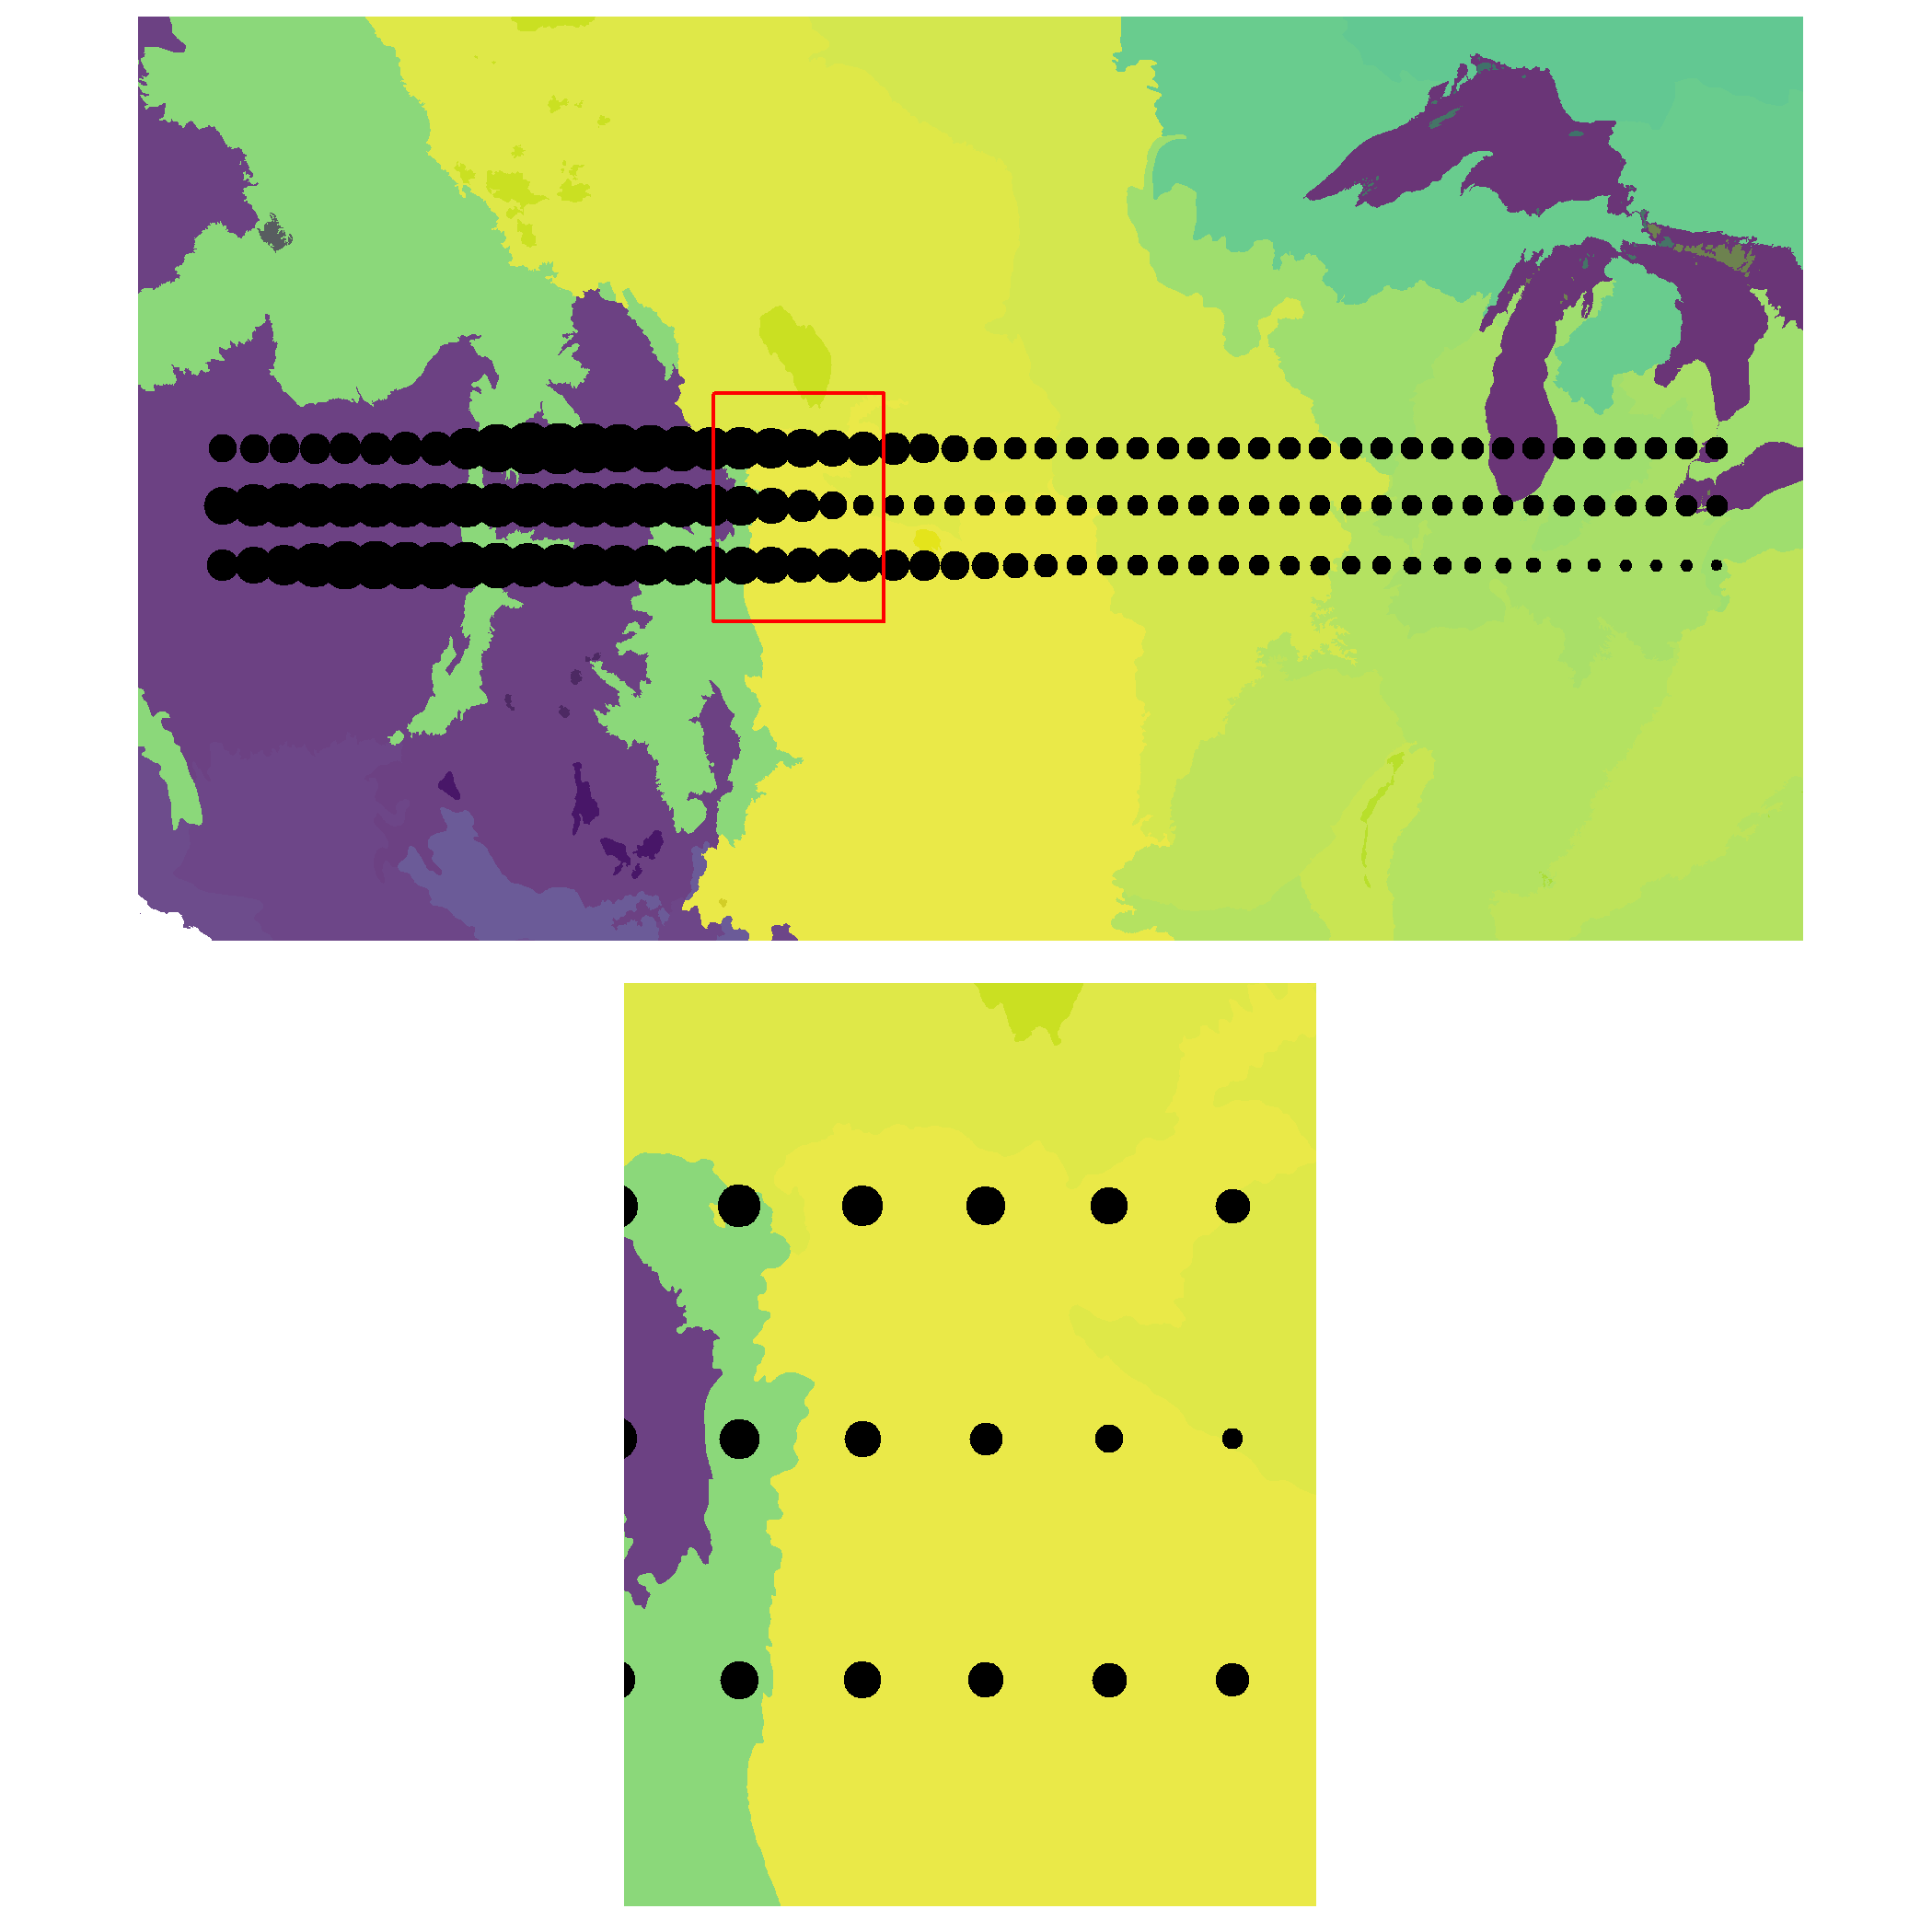
\includegraphics[width=0.85\linewidth]{./chapterFiles/fisherSpatial/figures/figsCalledInDiss/scaledFiInterpolated_year2010_zoom_East-West} \caption{No patterns of abrupt change detected in Fisher Information along three transects in year 2010}\label{fig:fiEcoregion}
\end{figure}
Upon initial investigation, there are no obvious signs of broad-scale patterns in FI across space (Fig. \ref{fig:fiEcoregion})\footnote{Size indicates value of Fisher Information (values are scaled and centered within transects). Red box (in top panel) indicates extent of bottom panel.}. If Fisher Information is an indicator of spatial regime boundaries, we should expect to see large changes in its value (in either direction) near the edges of functional spatial boundaries (e.g., at the boundaries of ecoregions). No clear regime changes appeared in areas where we might expect rapid changes (e.g., along the 105th meridian West, where a sharp change in altitude occurs).

Numerical investigation of the spatial correlation among adjacent transects also yielded no clear patterns. I did not identify any obvious correlation with changes in FI values and functional potential (using Omernick Ecoregion Level 2; see Fig. \ref{fig:fiEcoregion}). Rather than abrupt changes in Fisher Information I found graduaal changes (e.g., see results for years 2000 and 2010 in Figs. \ref{fig:fiEcoregion00},\ref{fig:fiEcoregion}).
\begin{figure}

\includegraphics[width=0.85\linewidth]{./chapterFiles/fisherSpatial/figures/figsCalledInDiss/scaledFiInterpolated_year2000_East-West} \caption{Fisher Information (scaled and centered; point size positively correlated with value) against ecoregion boundaries (EPA Level 2).}\label{fig:fiEcoregion00}
\end{figure}
\hypertarget{discussion-2}{%
\section{Discussion}\label{discussion-2}}

The Fisher Information measure was introduced as a method to avoid some analytical issues related to complex and noisy ecological data (Karunanithi et al., 2008), and has also been suggested as an indicator of \emph{spatial} regimes (Sundstrom et al., 2017). I found no evidence suggesting Fisher Information {[}Eq. \eqref{eq:fiDerivs}{]} can identify `spatial regimes'. Further, the absence of autocorrelation among spatially adjacent transects suggests Fisher Information may not be a realiable indicator of changes in bird community structure.

Although the Fisher Information equation {[}Eq. \eqref{eq:fiDerivs}{]} used in this study is a relatively straightforward and fairly inexpensive computational calculation, extreme care should be taken when applying this index to ecological data. Fisher Information is capable of handling an infinite number of inputs (variables), and given sufficiently low window size paramters, can technically calculate an index value for only two observations. It is important that the user understands the assumptions of identifying 'regime shifts; using Fisher Information, since the efficacy of this method has not been yet subjected to rigorous tests (but see \ref{resampling}). There are three primary assumptions required when using Fisher Information to estimate relative orderliness within ecological data (Mayer et al., 2007):\\
1. the order or state(s) (\(s\)) of the system is observable,
1. any observable change in the information observed in the data represents reality and the variables used in the analyses will not produce false negatives, and
1. changes in \(I\) presumed to be regime shifts do not represent the peaks of cyclic (periodic) patterns.

The first assumption is one of philosophical debate and is thus not controllable. To attempt to control for false negatives, the user should take caution in her choice of input variables. In the the case of a high dimensional data, relativization and/or variable reduction measures may be useful (Rodionov 2005). However, Fisher Information does not convey information on how specific variables relate to the calculated index. Finally, we can take measures to account for cyclic behavior in the data by ensuring integration periods capture at one full cycle of the system and, given sufficently high number of observations, increasing the integration period may also alleviate some issues related to irreducible error (white noise).

The lack of patterns identified using Fisher Information may be influenced by one or more of the following: (1) the Breeding Bird Survey data collection scheme was designed to estimate and track \textbf{species} trends and not changes in entire communities; (2) these data consist of \textless{} 50 time points, and for some BBS routes much fewer. Ecological processes affecting large regions in this study area (e.g., the Central Great Plains) operate on larger time scales (i.e., \textgreater\textgreater{} 50 points). A mismatch among the ecologically relevant scales and the temporal resolution and extent of our data may influence the ability of this index to capture large-scale changes in whole bird communities.

Aside from the typical biases associated with the BBS data (e.g., species detection probability, observer bias), there are additional considerations to be made when using these data to identify `spatial regimes'. Breeding Bird Survey routes are spaced apart so as to reduce the probability of observing the same individuals, but birds which fly (especially in large flocks) overhead to foraging or roosting sites have a higher probability of being detected on multiple routes. We have, however, removed these species (waders, shorebirds, waterfowl, herons) from analysis. Regardless, this study assumes there is potential for each unique BBS route to represent its own state. If routes were closer together, it is more probable that the same type adn number of species would be identified on adjacent routes. Therefore, if this method does not detect slight changes in nearby routes which occupy the same `regime', then it follows that the method is sensitive to loss or inclusion of new species, which are spatially bounded by geological and vegetative characteristics. What new information does this give us about the system? Fisher Information reduces and removes the dimensionality of these middle-numbered systems, which omits critical information.

Effective regime detection measures should provide sufficient evidence of the drivers and/or pressures associated with the identified regime shifts (Mac Nally et al., 2014). The Fisher Information index collapses a wealth of data into a single metric, thereby foregoing the ability to relate state variables to the observed changes in Fisher Information, unlike other dimension reduction techniques. For example, loadings, or the relative influence of variables on the ordinated axes, can be derived from a Principal Components Analysis--this cannot be achieved using Fisher Information. If Fisher Information clearly suggested a spatial regime boundary or shift, a before-and-after post-hoc analysis of the regional community dynamics might confirm the regime shift occurrence.

\hypertarget{efficacy-of-fisher-information-as-a-spatial-rdm}{%
\subsection{Efficacy of Fisher Information as a spatial RDM}\label{efficacy-of-fisher-information-as-a-spatial-rdm}}

This study found no evidence suggesting Fisher Information accurately and consistently detects spatial boundaries of avian communities. Rapid changes in either direction of Fisher Information is suggested to indicate of a regime shift (Mayer, Pawlowski, \& Cabezas, 2006, p. @eason\_evaluating\_2012). Although this interpretation has been applied to multiple case studies of Fisher Information, there is yet a statistical indicator to objectively identify these abrupt changes. After calculating the Fisher Information for each spatial transect (Fig. \ref{fig:ewRoutesUsedHere}) during each sampling year, I used pairwise correlation to determine whether spatial autocorrelation existed among pairs of spatial transects. If some set of points are close in space and are \emph{not} separated by some physical or functional boundary (e.g., an ecotone, high altitude rock formations), then the Fisher Infomration calculate should exhibit a relatively high degree of spatial autocorrelation that is consistent over time. It follows that the correlation coefficient of spatially adjacent transects should be similar, diverging only as the distance beteween the transects differs and/or a functional or physical boundary separates them.

Several questions remain regarding the efficacy of Fisher Information as a regime detection measure in both spatial and temporal data. If signals of regime shifts do exist, it is clearly not possible to identify them using visual interpretation. I also did not find evidence to suggest spatial autocorrelation of the calculations. I suggest future studies of Fisher Infomration focuses on temporal, rather than spatial data. Potential areas of research and questions include:
\begin{enumerate}
\def\labelenumi{\arabic{enumi}.}
\tightlist
\item
  Relationship of Fisher Information to likelihood ratio-based unsupervised change-point detection algorithms (e.g., ChangeFinder; Liu, Yamada, Collier, \& Sugiyama, 2013).\\
\item
  Sensitivity of Fisher Information to data quality and quantity {[}this is explored in Chapter \ref{resampling}{]}.
\item
  What, if any, advantages does FI have over other density estimation techniques?
\item
  Does FI provide signals in addition to or different than geophysical and vegetative (e.g.~LIDAR) observations (data)?
\end{enumerate}
\hypertarget{velocity}{%
\chapter{\texorpdfstring{Velocity (\emph{v}): using rate-of-change of system trajectory to identify abrupt changes}{Velocity (v): using rate-of-change of system trajectory to identify abrupt changes}}\label{velocity}}

\hypertarget{introduction-3}{%
\section{Introduction}\label{introduction-3}}

When, how and why ecological systems exhibit abrupt changes is a hallmark of modern ecological research, and changes which are unexpected and undesirable can have undesirable downstream consequences on, e.g., ecosytem services, biodiversity, and human well-being. Quantitatively detecting and forecasting these changes, however, has yet to be accomplished for most ecological systems (Chapter \ref{rdmReview}; Ratajczak et al., 2018). Moving from abrupt change methods requiring highly descriptive models and \emph{a priori} assumptions of the state variable responses to drivers to methods requiring few, if any, \emph{a priori} assumptions or knowledge is increasingly necessary for forecasting and managing complex ecosystems under an era of intensifying anthropogenic pressures.

A few broad classes of quantitative approaches exist for quantitatively identifying abrupt changes in complex ecosystems. First, one can use simple mathematical models to describe the system and statistically test for discontinuities in the observed variables (e.g., in coral reefs, Mumby, Steneck, \& Hastings, 2013). Although mathematical representations are ideal, very rarely are ecological systems easily and well-described by them and often fail to meet the assumptions of the model. Second, we can track changes in the mean or variance of state variables to identify departures from the norm (e.g., early-warning indicators such as variance and variance index, Brock \& Carpenter, 2006). Much like the mathematical modelling approach, these early-warning indicators have shown to be useful in some simple driver-response systems (e.g., lake eutrophication Carpenter, Brock, Cole, Kitchell, \& Pace, 2008), but are unreliable in other empirical systems (e.g., Perretti \& Munch, 2012; Dakos et al., 2012; Dutta et al., 2018). The last type of approach is the model-free approach {[}Dakos, Carpenter, et al. (2012); Ch. \ref{rdmReview}{]}. This group of abrupt change indicators can incorporate multiple state variables, and ideally requires no \emph{a priori} assumptions about the expected driver-response relationships, or even about the drivers at all. It is this class of abrupt change indicators to which this chapter contributes.

\hypertarget{tracking-ecosystem-trajectory-through-time-to-explore-system-dynamics}{%
\subsection{Tracking ecosystem trajectory through time to explore system dynamics}\label{tracking-ecosystem-trajectory-through-time-to-explore-system-dynamics}}
\begin{Shaded}
\begin{Highlighting}[]
\NormalTok{knitr}\OperatorTok{::}\KeywordTok{include_graphics}\NormalTok{(here}\OperatorTok{::}\KeywordTok{here}\NormalTok{(}\StringTok{"chapterFiles/velocity/figsCalledInDiss/lorenz3D.png"}\NormalTok{))}
\end{Highlighting}
\end{Shaded}
\begin{figure}
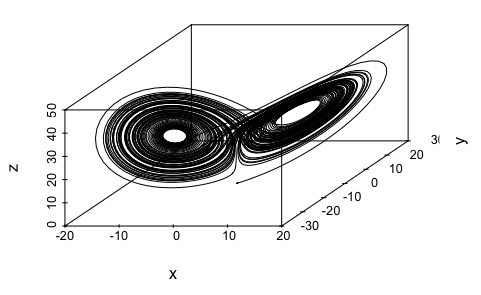
\includegraphics[width=0.85\linewidth]{/Users/jessicaburnett/Documents/GitHub/myDissertation/chapterFiles/velocity/figsCalledInDiss/lorenz3D} \caption{An example solution of the Lorenz ('butterfly') represented in 3-dimensional phase-space. Phase plots are typically used to visualize stable areas within a system's trajectory but reconstruction requires the difference models to be known and parameterized.}\label{fig:lorenz3D}
\end{figure}
\begin{Shaded}
\begin{Highlighting}[]
\NormalTok{knitr}\OperatorTok{::}\KeywordTok{include_graphics}\NormalTok{(here}\OperatorTok{::}\KeywordTok{here}\NormalTok{(}\StringTok{"chapterFiles/velocity/figsCalledInDiss/lorenz3D_timeseries.png"}\NormalTok{))}
\end{Highlighting}
\end{Shaded}
\begin{figure}
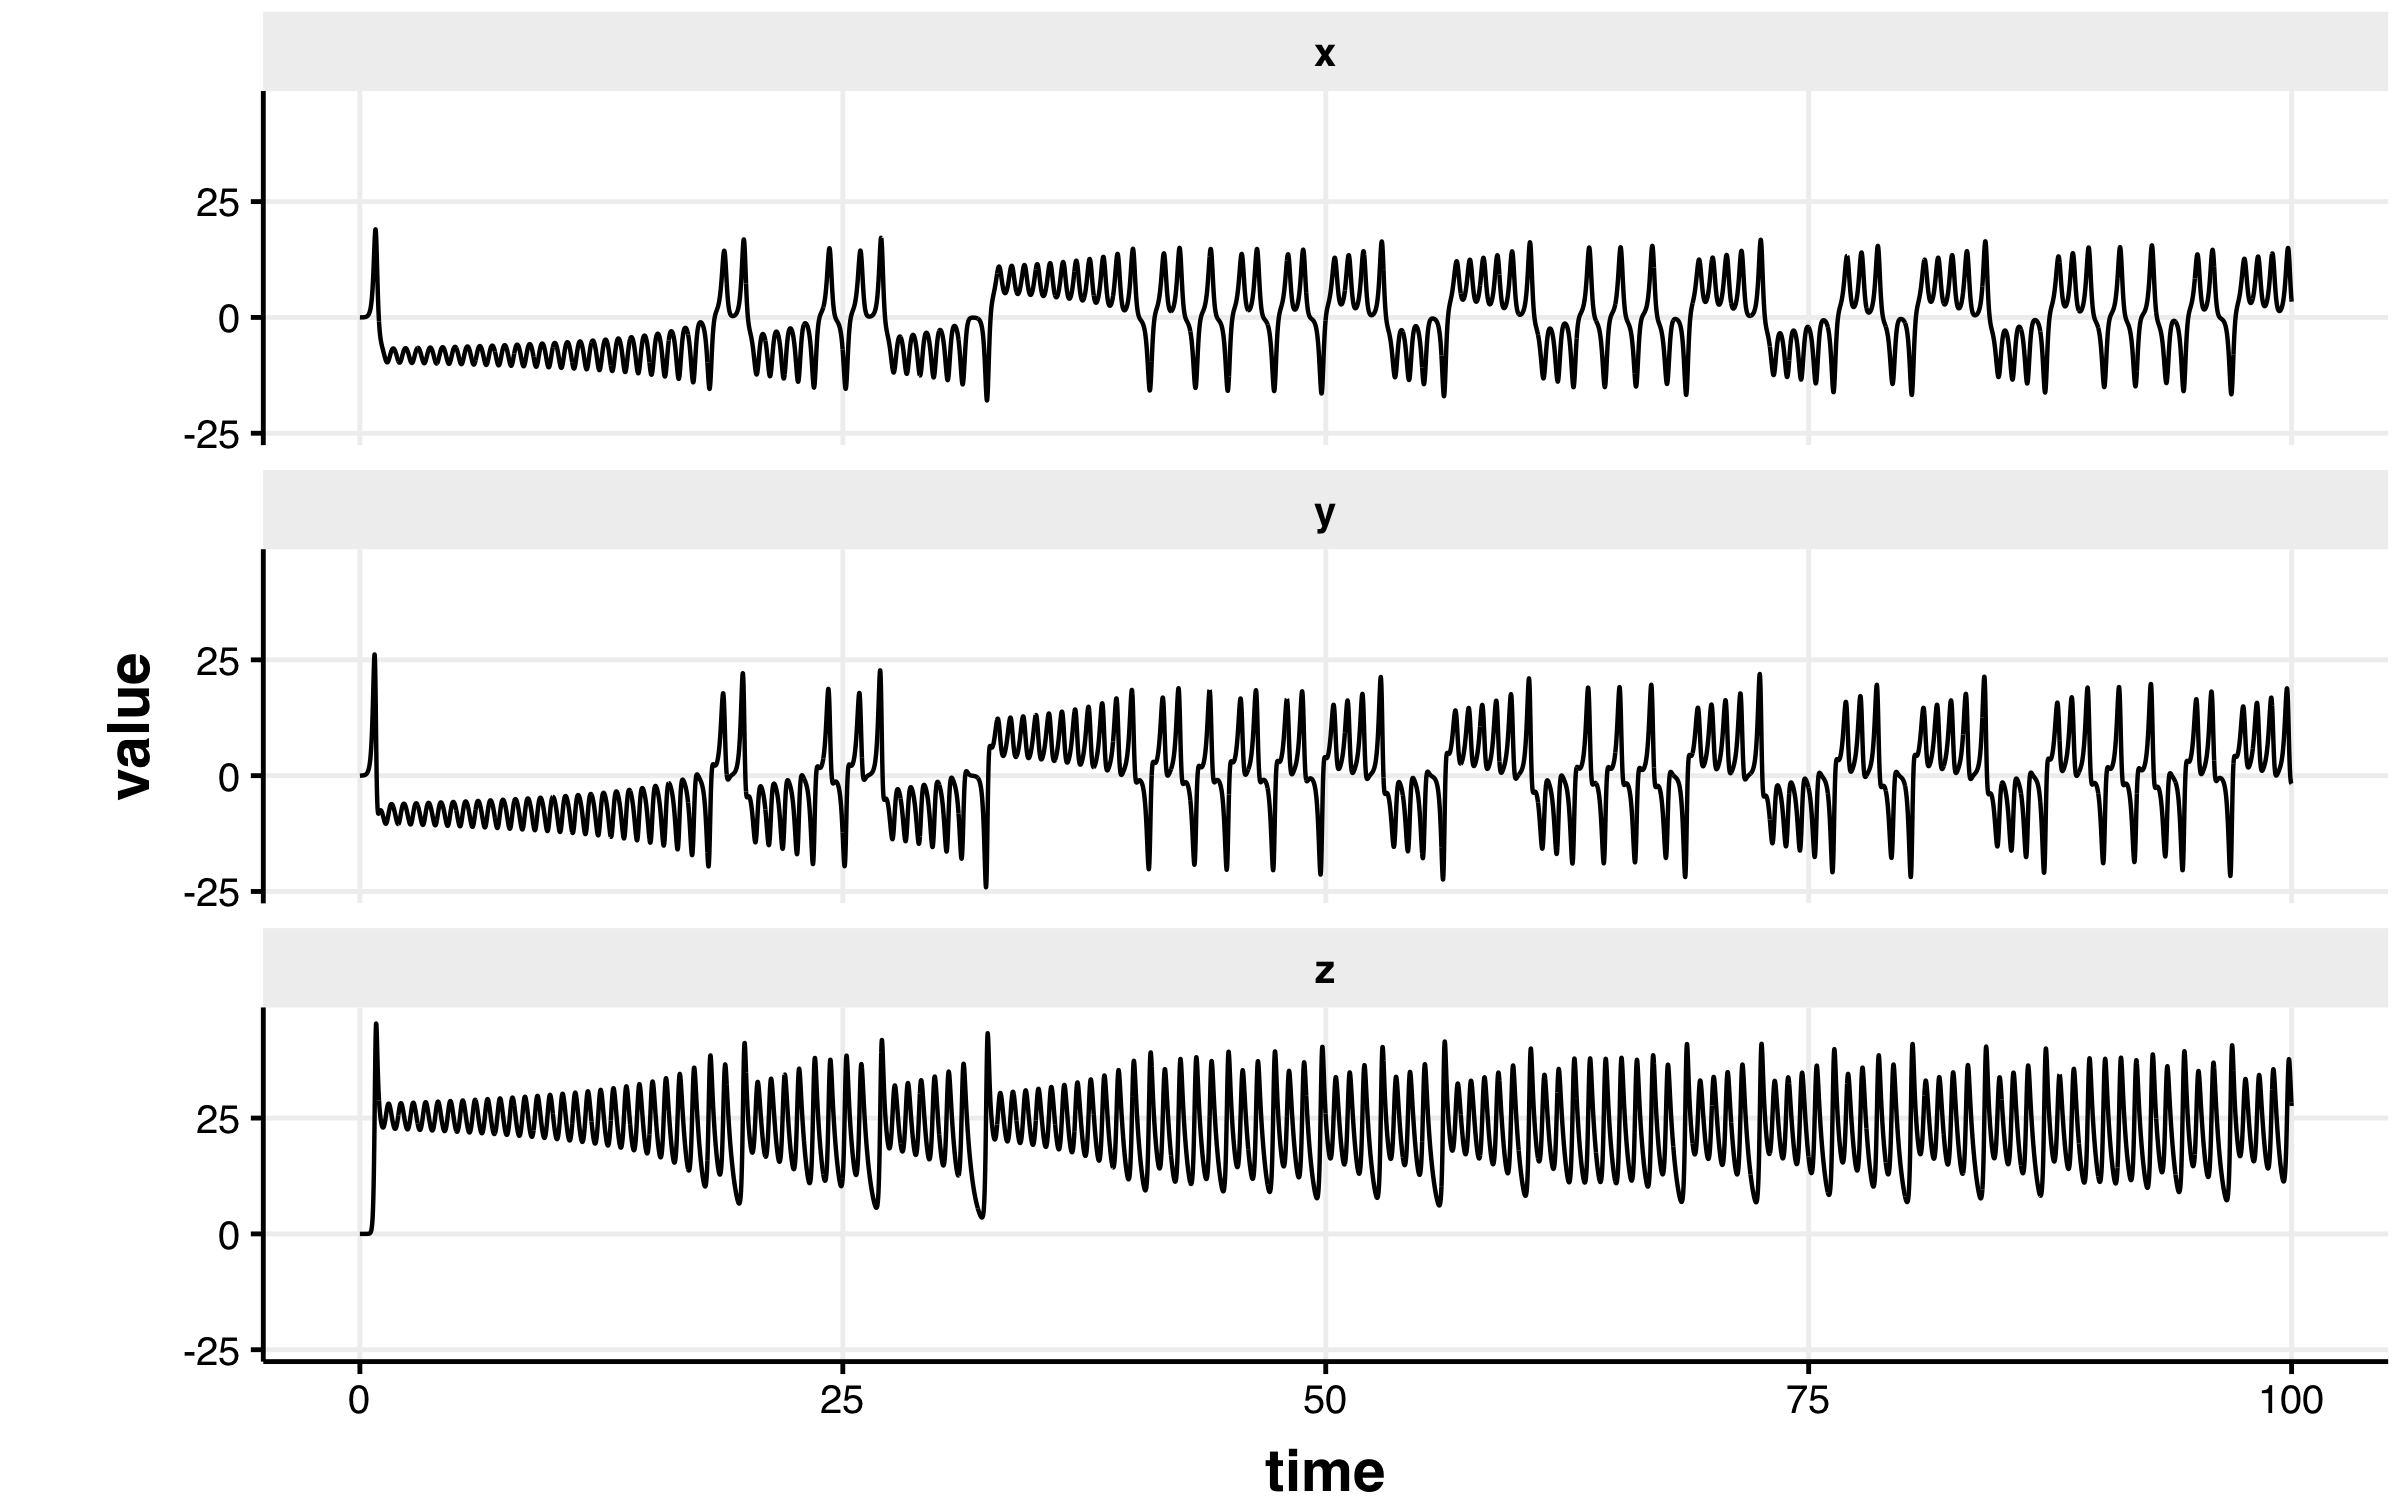
\includegraphics[width=0.85\linewidth]{/Users/jessicaburnett/Documents/GitHub/myDissertation/chapterFiles/velocity/figsCalledInDiss/lorenz3D_timeseries} \caption{An example solution of the Lorenz ('butterfly') represented in individual system compoents.}\label{fig:lorenz3Dts}
\end{figure}
A classic example of state-switching by a system is demonstrated in the Lorenz (`butterfly') attractor (Fig. \ref{fig:lorenz3D}; Takens, 1981). This phase plot (Fig. \ref{fig:lorenz3D}) provides an informative visual of the behavior of a chaotic system manifesting two attractors. Although the periodic, attractor behaviors are made clear when examining the time series of each dimension (Fig \ref{fig:lorenz3Dts}), identifying such behaviors in additional dimensions becomes increasingly difficult.

System behavior/trajectory in phase space are used often in dynamical systems theory and systems ecology to make inference regarding system behavior and dynamics, but phase space (trajectory) dynamics are not commonly applied outside theoretical studies as a tool for ecological data analysis (c.f. Sugihara et al., 2012 for an example of phase-space reconstruction using Taken's theorem of ecological time series). Some methods of attractor reconstruction have been applied to environmental data (e.g., individual time series of fisheries stocks, climate, stock market; Sugihara et al., 2012; Ye et al., 2015), yet they \textbf{do not incorporate the dynamics of whole-systems}. Model-free methods for exploring and describing the dynamics of whole (i.e.~\(>1\) variable) ecological systems are restricted to the commonly-applied dimnesion reduction techniques and clustering algorithms (e.g., Principal Components Analysis, K-means clustering). In fact, this is true of many abrupt change and regime shift indicators.

\hypertarget{rate-of-change-as-an-indicator-of-abrupt-change-in-the-system-trajectory}{%
\subsection{Rate of change as an indicator of abrupt change in the system trajectory}\label{rate-of-change-as-an-indicator-of-abrupt-change-in-the-system-trajectory}}

How quickly a system switches states {[}e.g., moving from attractor to another; \ref{fig:lorenz3D}{]} may yield insights into the responses of ecological systems to perturbations (e.g., anthropogenically induced pressures such as climate change, urbanization) and community shifts (e.g., species introductions or extinctions, shifts in dominance). For example, Beck et al. (2018) tracked rate of change using chord distances---a data transformation for positive values and which is suitable prior to ordination analysis---to capture abrupt changes in community composition of a temperate, paleodiatom community. Chord distance, however, is greatest when the observations among data rows (e.g., time, location) have no species in common. In other words, this measurement may be most useful in high community turnover conditions. Identifying alternative numerical methods for estimating system rates of change may be when the system does not exhibit, for example, high degrees of turnover.

Rate of change (ROC, often represented as \(\Delta\)) is a term used for various measures which describe the relationship among to variables, measuring the change in one variable relative to another. As a refresher ROC is represented as \textbf{speed} (\(\textbf{S}\)) or \textbf{velocity} (\(\textbf{V}\)), where (\(\textbf{S}\)) is the adirectional magnitude (i.e.~it is a scalar) of the displacement of an object over unit time and \(\textbf{V}\) describes both the direction and magnitude (i.e.~it is a vector) of the object's movement in spacetime. \(\textbf{S}\) is a scalar taking values of \(\geq0\) and \(\textbf{V}\) can take any value between \(-\infty\) and \(\infty\). For example, consider a car travelling at a constant speed of \(50\frac{km}{h}\) around along a hilly landscape, where it is ascending and descending hills. Although \(\textbf{S}\) is constant, \(\textbf{V}\) changes in a sunusoidal fashion, where \(\textbf{V}\) is \(\textbf{V}>0\) when ascending, \(\textbf{V}<0\) when descending, and \(\textbf{V}\approx0\) at in the valleys and at the peaks of the hills. Although \(\textbf{S}\) is useful when estimating other scalar quantities (e.g., \(\frac{miles}{gallon}\)), given a starting and/or final position in space, \(\textbf{S}\) is not informative of its the path travelled.

\hypertarget{aims-1}{%
\subsection{Aims}\label{aims-1}}

Here, I propose a method which simply describes the rate of change behavior of system dynamics in phase space: \textbf{velocity}, \(V\). An alternative to other complicated, model-free approaches (e.g., Fisher Information; Cabezas \& Fath, 2002), the velocity metric allows one to examine the behavior of an entire system along its trajectory
(through space or time) without having to reconstruct the pahse space. The ability to handle noisy and high-dimensional data and the lack of subjective parameters in calculating the metric makes this method an ideal alternative to existing early warning indicators and phase-space reconstruction methods.

I first describe the steps for calculating this new metric (\(v\)), as both a dimension reduction technique and abrupt change indicator. Although this is the first instance of this calculation to, alone, be suggested as a regime detection metric, it has been used as part of a larger series of calculations of the Fisher Information metric {[}see Ch. \ref{fiGuide}{]}, first introduced in Fath et al. (2003). I use this theoretical system to present baseline estimates of the expected behavior of \(v\) under various scenarios of changing mean and variability in a theoretical, discussing the contexts under which this metric may signal abrupt changes. Finally, I explore the utility of this metric in identifying known regime shifts in an empirical paleoecological time series data.

\hypertarget{analytical-approach}{%
\subsection{Analytical approach}\label{analytical-approach}}

I first describe the steps for calculating velocity by constructing a simple, two-variable system which exhibits only a rapid, discontinuous change in the means of the state variables. I next vary the mean and variance of the state variables of this system to demonstrate baseline expectations for the behavior of velocity under a simple rapid shift scenario. Next, I construct a second model system similar to the first, but one which exhibits a non-discontinuous rapid change in the state variables. The purpose of this section is three-fold. First, I demonstrate how velocity behaves when the system undergoes varying degrees of change (e.g., slow change versus nearly discontinuous, rapid). Second, I concurrently identify baseline expectations of velocity under varying conditions of mean and variability of the state varilbes before and after a shift. Third, by introducing a smoothing function to the rapid shift, we gain an understanding of how process variability (noise) impacts the shift detectability by the velocity metric. Finally, I calculate the velocity of an empirical, paleolitic freshwater diatom community time series to demonstrate the utility of the velocity metric in highly noisy, high dimensional, and irregularly-sampled data.

\hypertarget{steps-for-calculating-velocity-v}{%
\section{\texorpdfstring{Steps for Calculating velocity, \(v\)}{Steps for Calculating velocity, v}}\label{steps-for-calculating-velocity-v}}

In this section, I first demonstrate the calculations of velocity using a very simple, two-variable toy system. The first system exhibits a rapid shift at a single point in time, where mean and variance are constant before and after the shift point. I demonstrate the signals achieved with and the variability within the \(v\) calculation by exploring a number of scenarios of this simple system. For the examples in this section, observations of \(x_i\) are randomly drawn from distribution \(x_i\sim Normal(\mu, \sigma)\), where \(\mu\) is the mean and \(\sigma\) is the standard deviation.
\begin{figure}
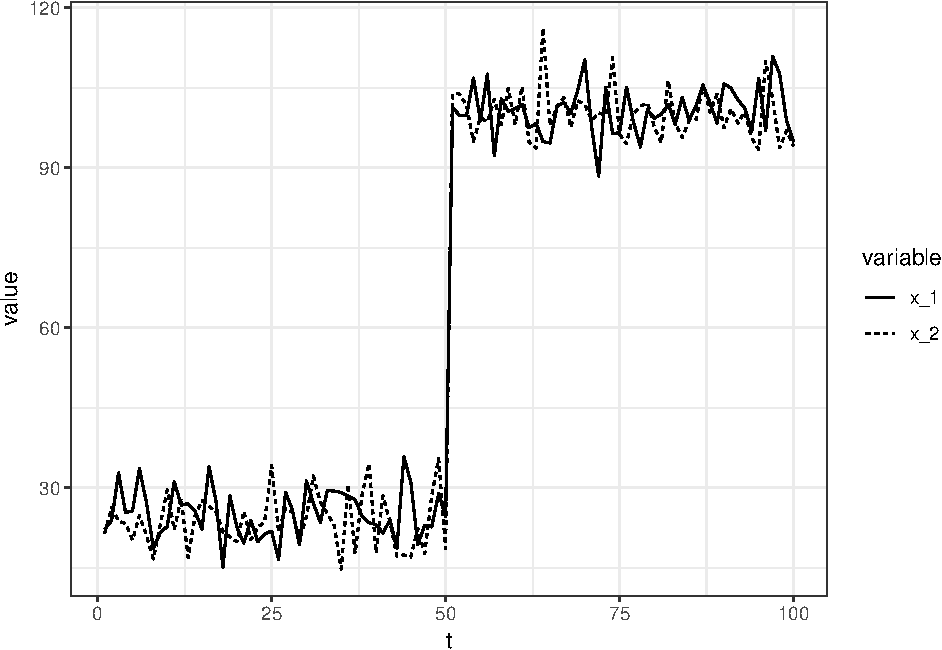
\includegraphics[width=0.85\linewidth]{_myDissertation_files/figure-latex/sysEx-1} \caption{The 2-variable discrete time toy system used to demonstrate steps for calculating system velocity. Each variable, $x$, is drawn from a normal distribution with means that change at $t = 50$. State variables have constant standard deviation, $\sigma = 5$.}\label{fig:sysEx}
\end{figure}
Consider a system (Fig. \ref{fig:sysEx}) with \(N\) state variables (\(x_i\)), with observations taken at time points, \(t\). System velocity is calculated as the cumulative sum over time period \(t_0\) to \(t_j\), as the total change in all state variables, \{\(x_1 ...x_N\)\}, between two adjacent time points, e.g., \(t_j\) and \(t_{j+1}\), denoted \(t_{j,j+1}\). I use this simple, two-variable system to demonstrate how \emph{velocity} is calculated. The system comprises variables \(x_1\) and \(x_2\), with observations occurring at each time point \(t = {1,2,3,...100}\). First, we calculate the change in each state variable, \(x_i\), between two adjacent points in time, \(t_j\) and \(t_{j+1}\), such that the difference, \(x_{t_{j+1}} - x_{t_j}\) is assigned to the latter time point, \(t_{j+1}\). For example, in our toy data, we use observations at time points \(t = 1\) \& \(t=2\) (Fig. \ref{fig:sysEx2}). For all examples in this chapter, the state variables \(x_1\) and \(x_2\) were drawn from a normal distribution (using function \emph{rnorm}), with parameters \(\bar{x}_i\) (mean) and \(\sigma_i\) (sd) for 100 time steps, \(t\). The regime shift in this system occurs at \(t=50\), where a shift in either or both \(\bar{x}_i\) or \(\sigma_i\).
\begin{figure}
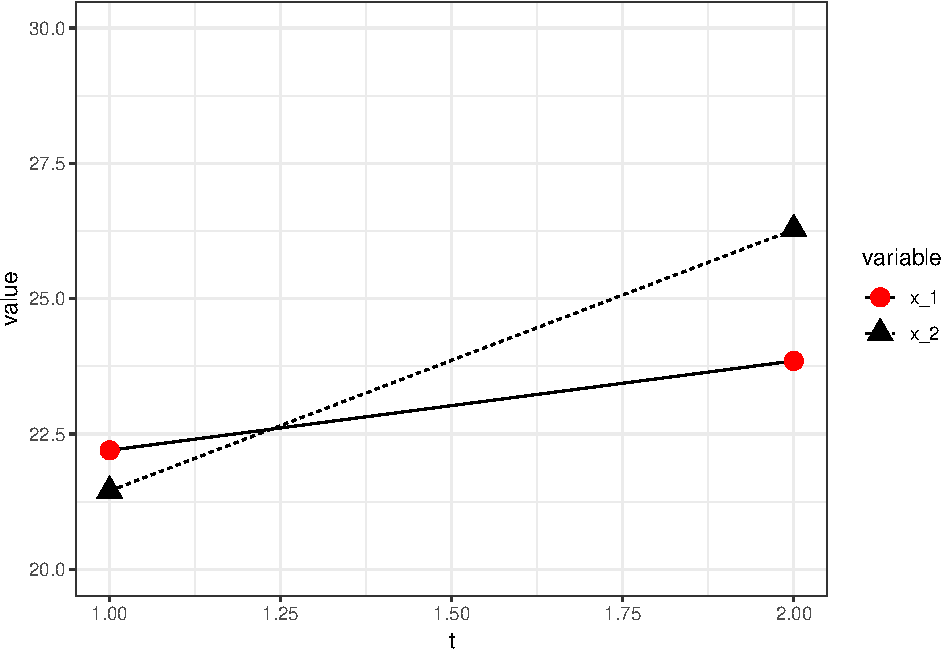
\includegraphics[width=0.85\linewidth]{_myDissertation_files/figure-latex/sysEx2-1} \caption{Data used to calculate velocity at the first two time points, $t_1$ and $t_2$.}\label{fig:sysEx2}
\end{figure}
\hypertarget{steps-for-calculating-v}{%
\subsection{\texorpdfstring{Steps for calculating \(v\)}{Steps for calculating v}}\label{steps-for-calculating-v}}

\hypertarget{step-1-calculate-delta-x_i}{%
\subsubsection{\texorpdfstring{Step 1: Calculate \(\Delta x_i\)}{Step 1: Calculate \textbackslash Delta x\_i}}\label{step-1-calculate-delta-x_i}}

The first step is to calculate the change in values for each state variables, \(x_i\), between two consecutive time points {[}e.g., from time \(t\) to \(t+1\) for the discrete-time system; Fig. \ref{fig:sysEx2}; Eq. \eqref{eq:diffX}{]}:
\begin{equation}
\Delta x_i = x_{i(t+1)} - x_{it} 
\label{eq:diffX}
\end{equation}
Note that \(\Delta x_i\) can take any value between \(-\infty\) and \(\infty\).

\hypertarget{step-2-calculate-distance-travelled-s}{%
\subsubsection{\texorpdfstring{Step 2: Calculate distance travelled, \(s\)}{Step 2: Calculate distance travelled, s}}\label{step-2-calculate-distance-travelled-s}}

Next, we calculate the total change in the multivariable system as a function of the change in all state variables \(x_i\). First, we calculate \(\Delta s\) as the square root of the sum of squares of the changes in all state variables per Pythagora's theorem (Eq. \eqref{eq:ds}):
\begin{equation}
\Delta s = \sqrt{\sum{\Delta x_i^2}}
\label{eq:ds}
\end{equation}
Although \(\Delta s\) represents the absolute change in the system between consecutive points in time, this measure is not yet relative along the system's trajectory. To create a relative value we next calculate the total distance travelled along the system trajectory, \(s\), as the cumulative sum of \(\Delta s\) (Eq. \eqref{eq:ds}) since the first observation, such that a cumulative sum is calculated for every \(t\) over the interval \([0,T]\) (Eq. \eqref{eq:s}):
\begin{equation}
s_T = \Sigma_{t=0}^{T}{\Delta s}) 
  \label{eq:s}
\end{equation}
\begin{figure}
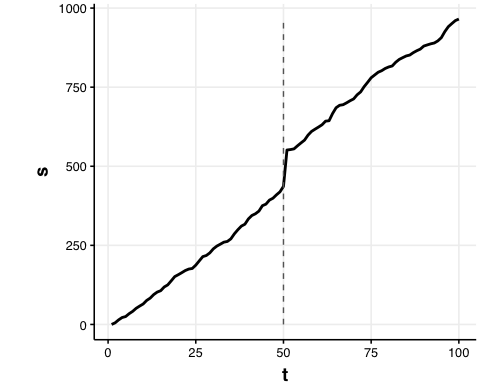
\includegraphics[width=0.85\linewidth]{_myDissertation_files/figure-latex/sysExs-1} \caption{Distance travelled, $s$, for the 2-species toy system.}\label{fig:sysExs}
\end{figure}
We now have a single measure, \(s_T\) {[}hereafter referred to as \(s\); Eq. \eqref{eq:s}{]} at each discrete point in time in our \(N\)-dimensional system (Fig. \ref{fig:sysExs}). It should be noted that \(s\)(Fig. \ref{fig:sysExs}) is monotonically increasing since the value of \(\Delta s\) (Eq. \eqref{eq:ds}) is a sum of squares. Although discussed in a later section, it is important to note that \(s\) is not unitless---that is, \(s\) has units of the state variables, \(x_i\). For example, if our 2-variable toy system represents biomass, then the units of \(s\) represents the cumulative absolute change in biomass of the entire system.

\hypertarget{step-3-calculate-velocity-v-or-fracdelta-sdelta-t}{%
\subsubsection{\texorpdfstring{Step 3: Calculate velocity, \(v\) (or \(\frac{\Delta s}{\Delta t}\))}{Step 3: Calculate velocity, v (or \textbackslash frac\{\textbackslash Delta s\}\{\textbackslash Delta t\})}}\label{step-3-calculate-velocity-v-or-fracdelta-sdelta-t}}

Finally, we calculate the \textbf{system velocity}, \(v\) (or \(\frac{\Delta s}{\Delta t}\)), by first calculating the change in \(s\) (Eq. \eqref{eq:s}), and then divide by the total time elapsed between consecutive sampling points:
\begin{equation}
 v = \frac {s_{t+1}-s_{t}}{\Delta t} 
\label{eq:velocity}
\end{equation}
\begin{figure}
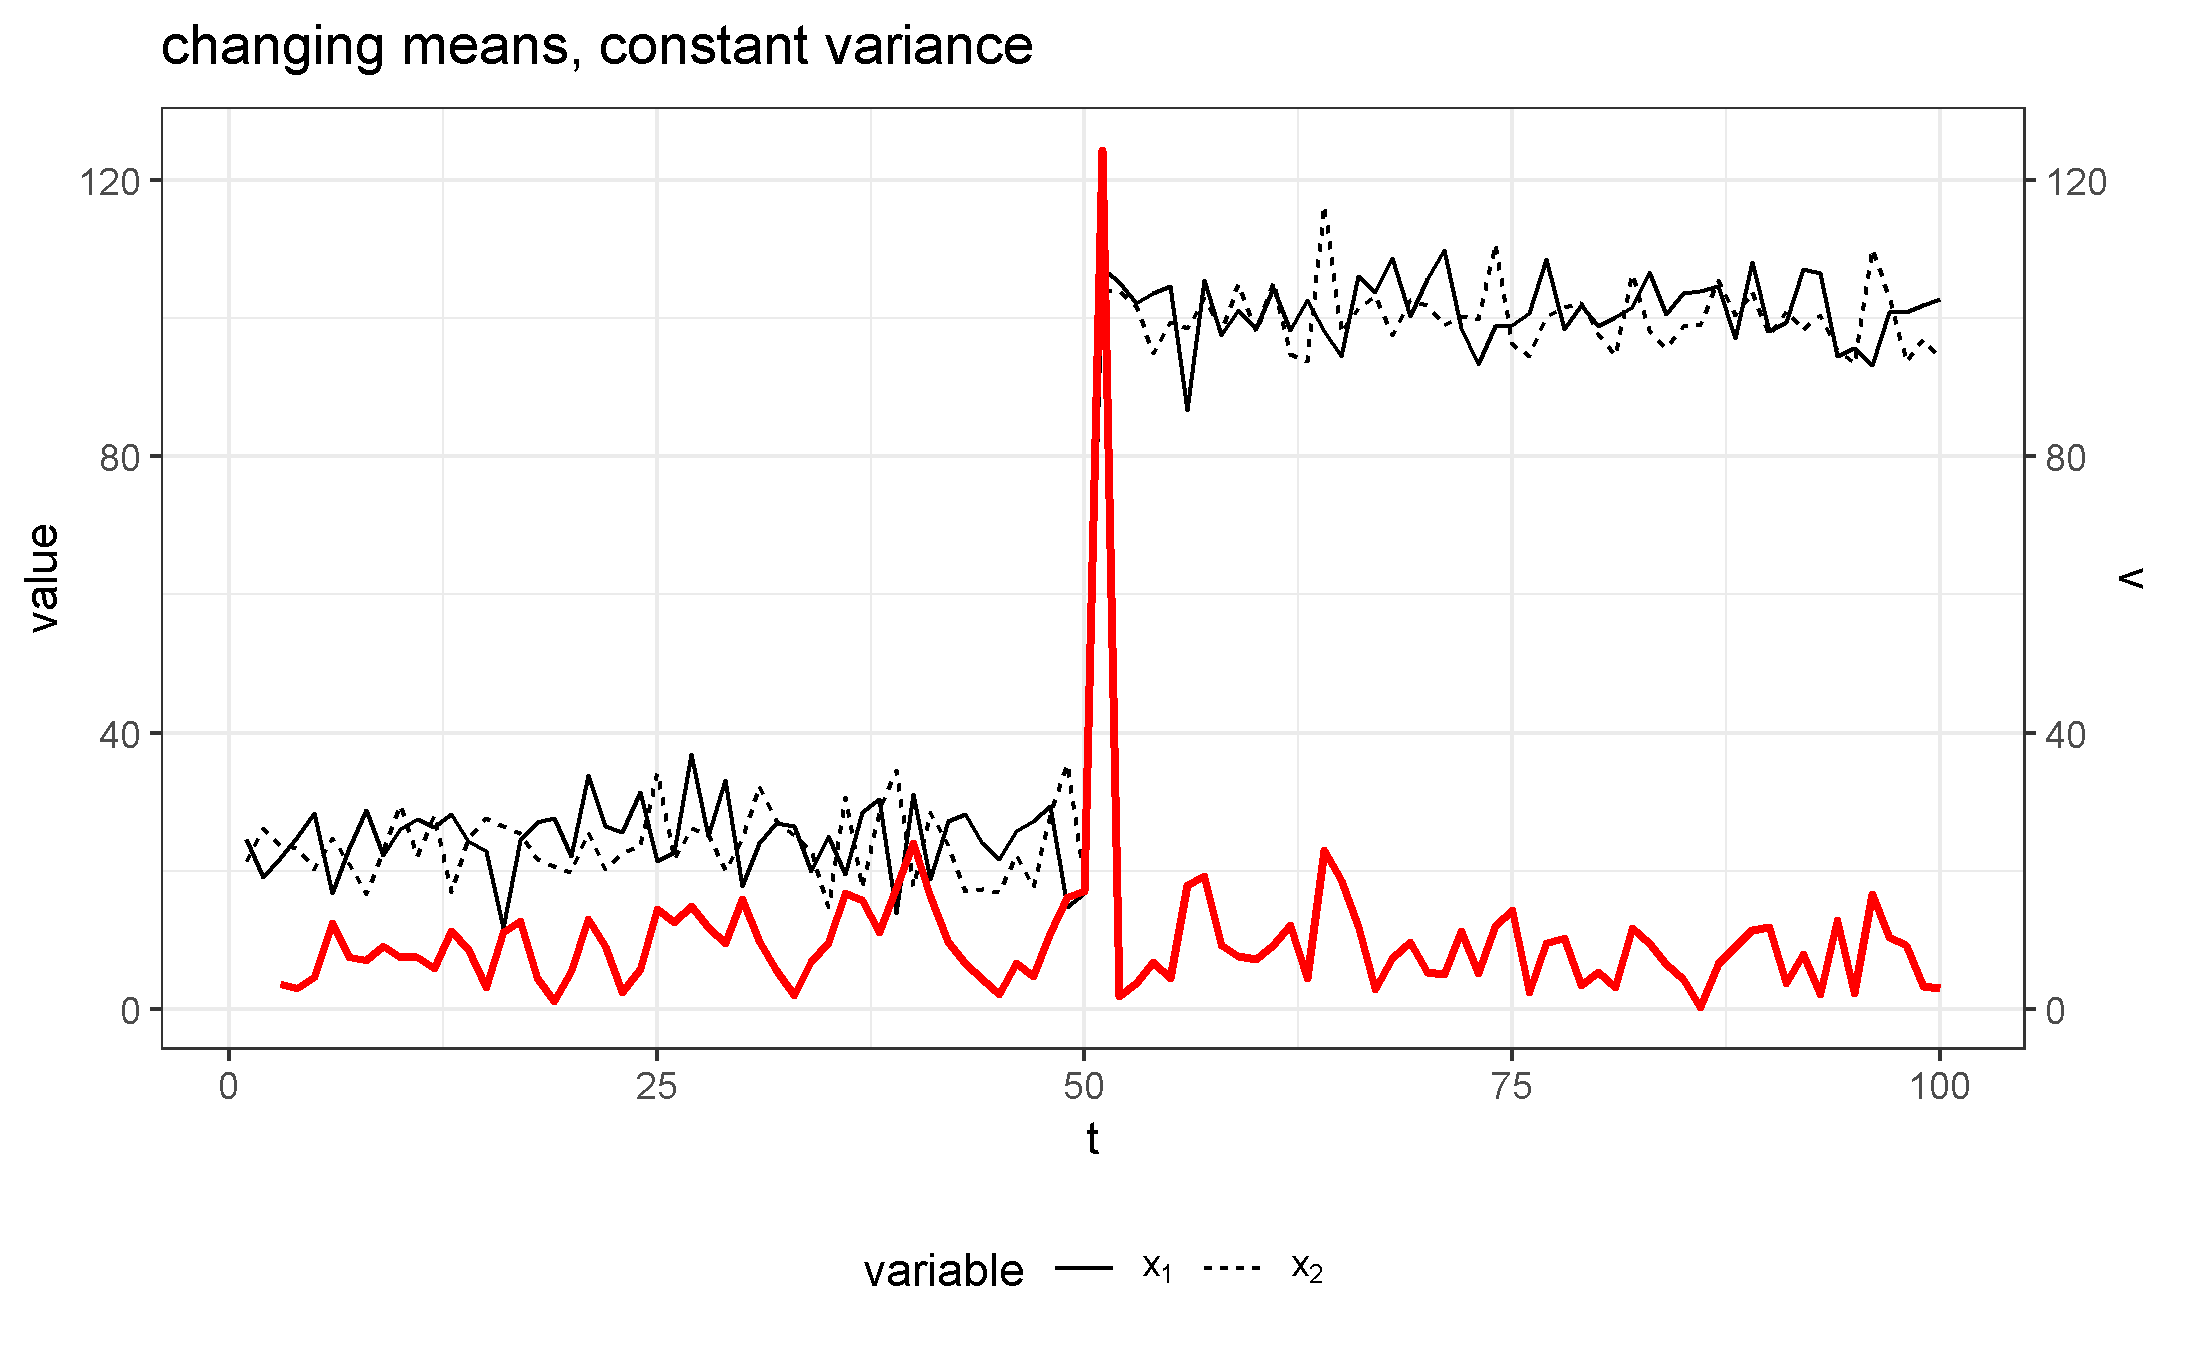
\includegraphics[width=0.85\linewidth]{/Users/jessicaburnett/Documents/GitHub/myDissertation/chapterFiles/velocity/figsCalledInDiss/velocitySysEx1} \caption{System change ($s$) and velocity ($v$) of the model system over the time period. Constant means ($\bar{x}_{pre}=25$, $\bar{x}_{post}=10$) and sharp change in variance for both state variables, $\sigma =5$.}\label{fig:velocSysEx1}
\end{figure}
\begin{table}[t]

\caption{\label{tab:distTab}Steps outlined for calculating system velocity, $v$, using the 2-variable toy data as an example.}
\centering
\begin{tabular}{ccccccccc}
\toprule
t & $x_1$ & $x_2$ & $\Delta x_1$ & $\Delta x_2$ & $\Delta t$ & $\sqrt(\sum_{i=1}^N \Delta x_i^2) $ & $s$ & $v$\\
\midrule
1 & 22.198 & 21.448 &  &  &  &  &  & \\
2 & 23.849 & 26.284 & 1.651 & 4.836 & 1 & 5.111 & 5.111 & \\
3 & 32.794 & 23.767 & 8.944 & -2.518 & 1 & 9.292 & 14.403 & 9.292\\
4 & 25.353 & 23.262 & -7.441 & -0.504 & 1 & 7.458 & 21.861 & 7.458\\
5 & 25.646 & 20.242 & 0.294 & -3.020 & 1 & 3.035 & 24.895 & 3.035\\
\bottomrule
\end{tabular}
\end{table}
The numerical results for each step in the calculation of velocity {[}Eq. \eqref{eq:velocity}{]} is demonstrated using the first five time points of our toy system (Fig. \ref{fig:sysEx}) in Table \ref{tab:distTab}.

\hypertarget{velocity-v-performance-under-a-discontinuous-transition}{%
\section{\texorpdfstring{Velocity \emph{v} performance under a discontinuous transition}{Velocity v performance under a discontinuous transition}}\label{velocity-v-performance-under-a-discontinuous-transition}}

I used simulation techniques to determine the baseline expectations of the performance of velocity \(v\) under varying degrees of rapid shifts in the mean and variance of the toy system. The toy system in this section undergoes a discontinuous shift at \(t = 50\) (see \ref{Fig:sysEx}). If the system undergoes a rapid and discontinuous change in one or more state variables, the velocity, beacuse it is a rate of change, may \(\rightarrow \infty\) as \(\Delta t \rightarrow 0\). Therefore, it is important to understand the degree to which

, while varying two each of the following system parameters at the regime shift:
- \(\bar{x}_1\), increase in the mean value of \(x_1\) at \(t=50\)\\
- \(\sigma_1\), change in variance of \(x_1\) at \(t=50\)

Simulations consisted of 10,000 random samples drawn from the normal distribution for each paramter, I randomly drew the toy system samples 10,000 times under increasing values of \(\bar{x}_1\) and \(\sigma_1\). To identify patterns in the influence of paramter values on velocity, I present the mean values of \(v\) across all simulations, with confidence intervals of \(\pm 2\) standard deviations. As mentioned above, the state variables \(x_1\) and \(x_2\) were drawn from a normal distribution (using function \emph{rnorm}), with parameters \(\bar{x}_i\) (mean) and \(\sigma_i\) (sd) for 50 time steps, \(t\).

\hypertarget{velocity-under-varying-degrees-of-varying-post-shift-mean}{%
\subsubsection{Velocity under varying degrees of Varying post-shift mean}\label{velocity-under-varying-degrees-of-varying-post-shift-mean}}

I examined the influence of the magnitude of change in \(x_1\) in the period before (pre; \(t <50\)) and after (post; \(t \geq 50\)) by varying the mean parameter, \(\bar{x}_1\) in the set \(W=\{25,30,35,...100 \}\) (Figs. \ref{fig:simVplot1},\ref{simVplot2}). As expected, the magnitude of \(v\) increases linearly as the total difference between \(\bar{x}_{1_{pre}}\) and \(\bar{x}_{1_{post}}\) increases (\ref{fig:simVplot2}). This is not surprising because \(s\) increases as the total change in abundance across the entire sytem increases (Eq. \eqref{eq:s}). Consequently the potential of \(v\) also increases with total state variable values (e.g.~abundance, biomass). The linear relationship among \(v\) and total state variable values indicates that while \(v\) is capable of identifying large shifts in data structure, it may fail to identify subtle changes (i.e.~lower effect sizes).
\begin{figure}
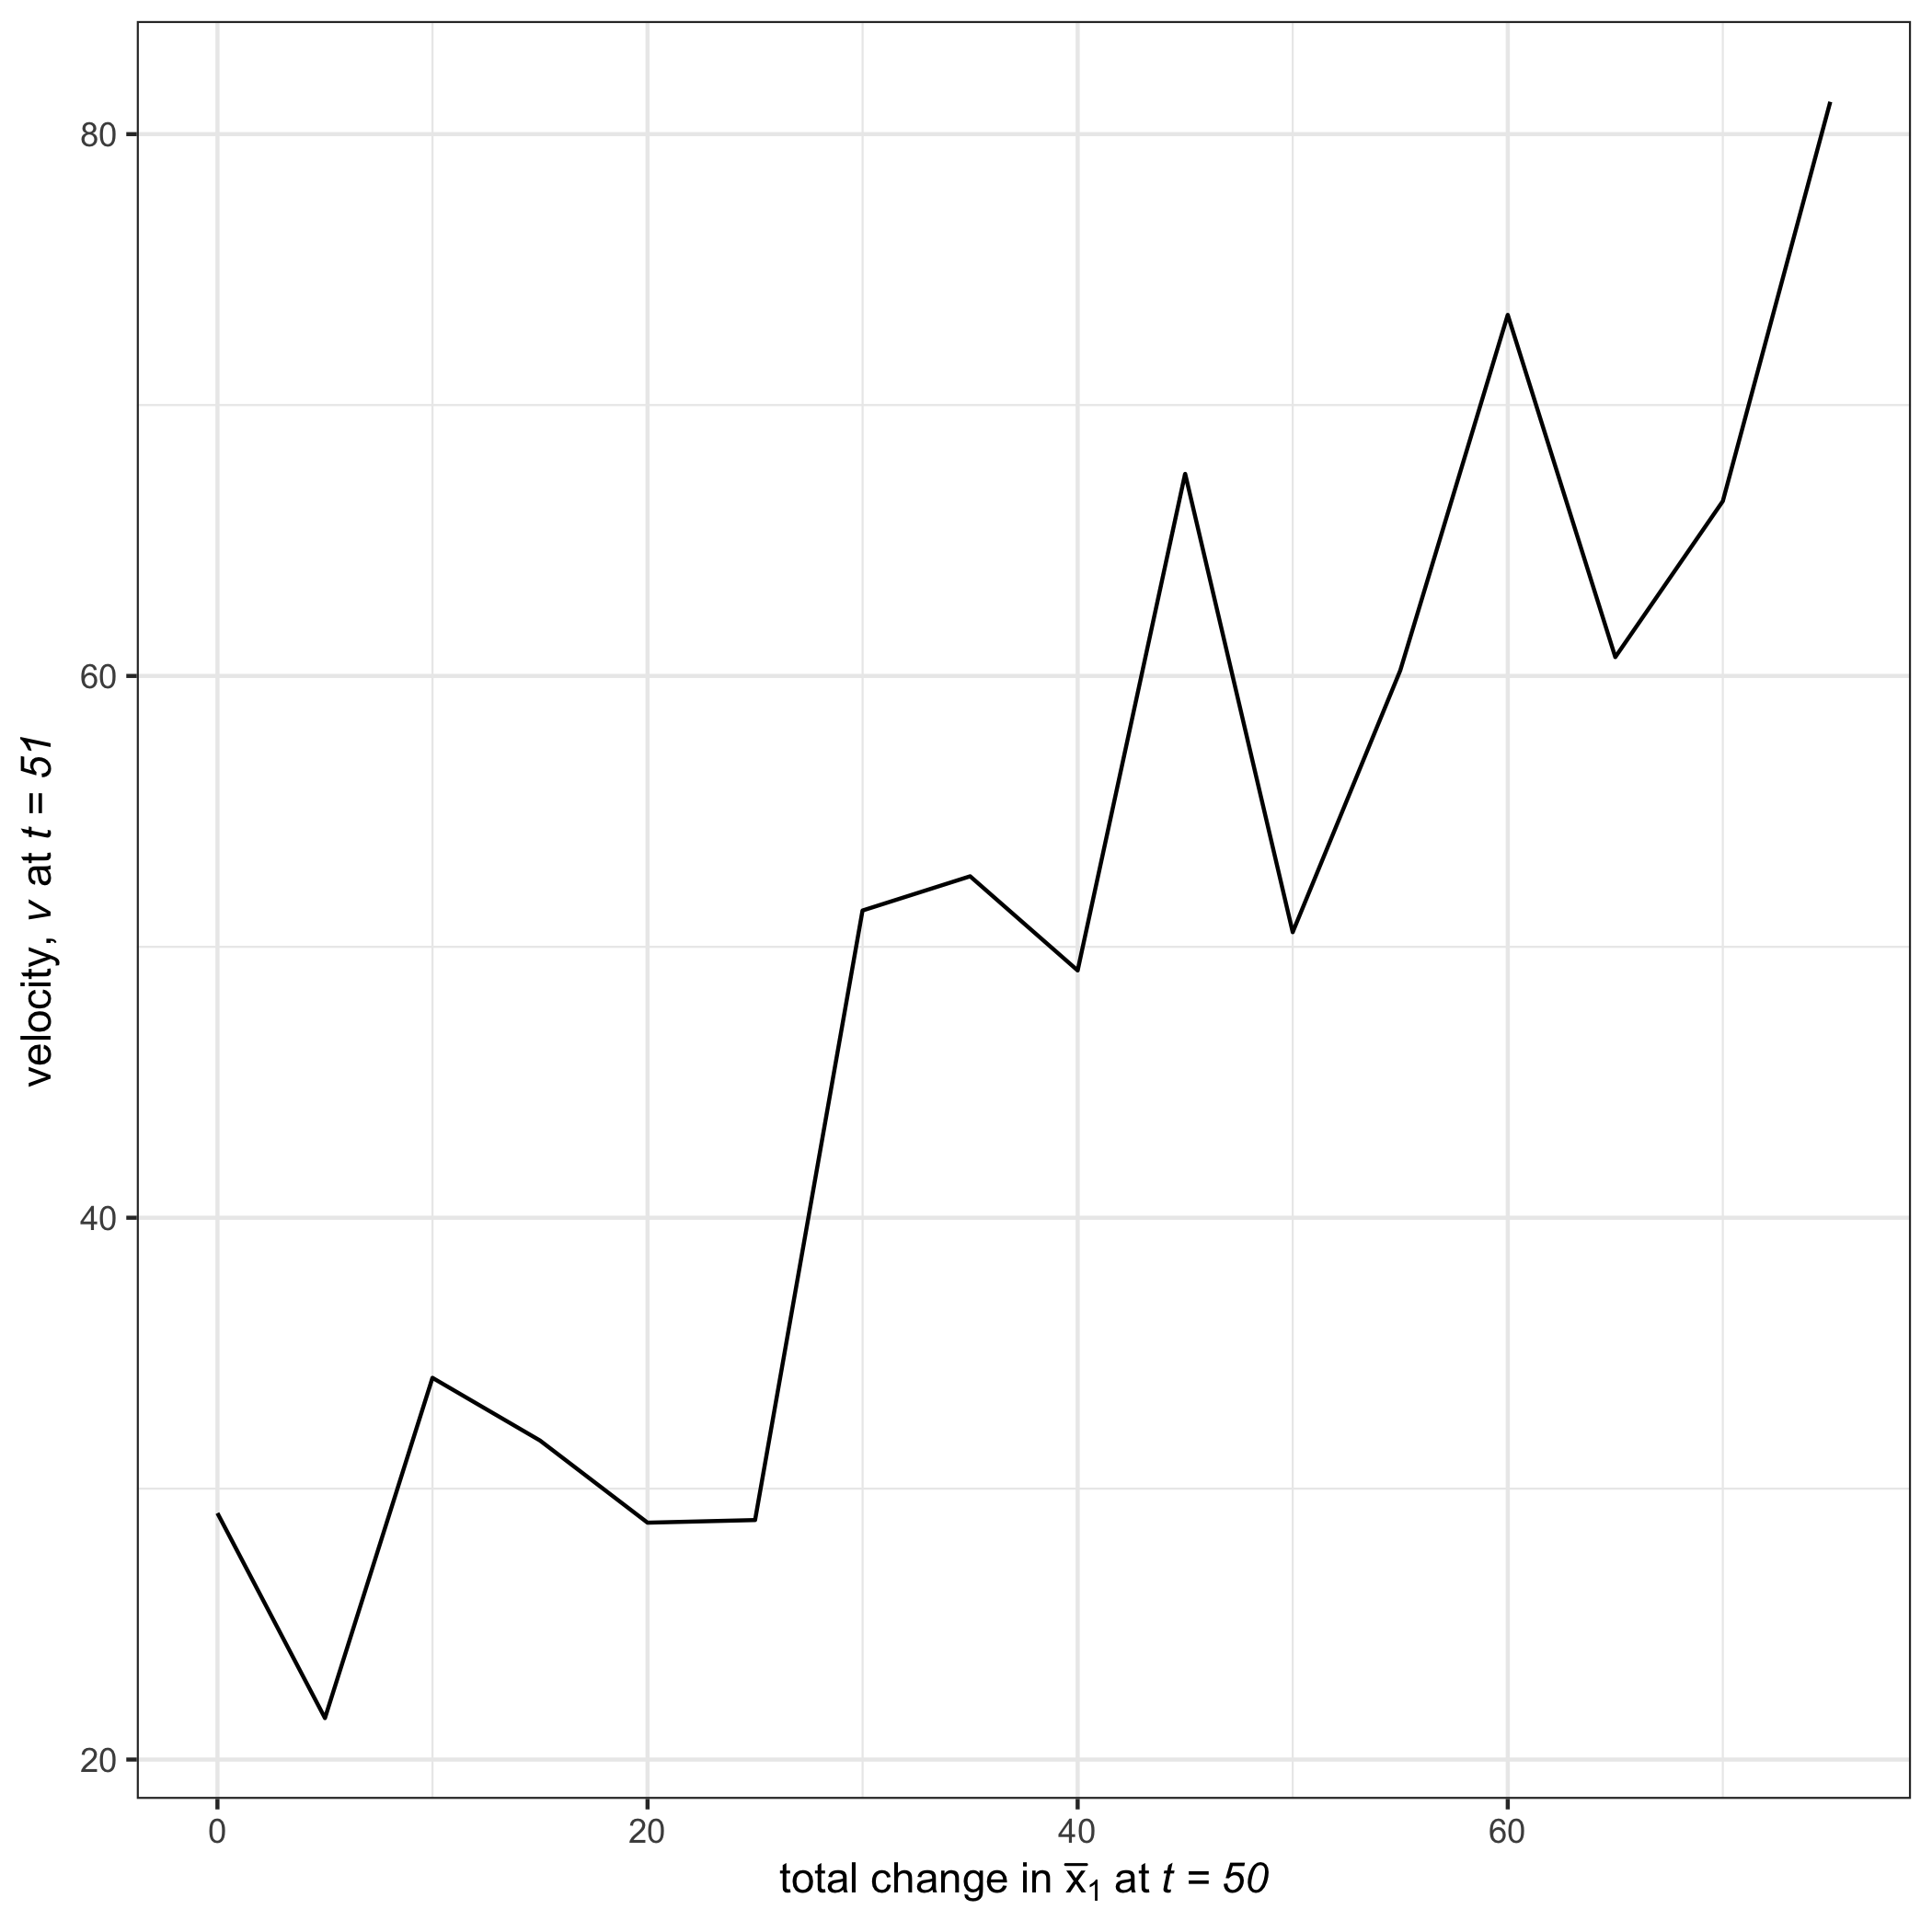
\includegraphics[width=0.85\linewidth]{/Users/jessicaburnett/Documents/GitHub/myDissertation/chapterFiles/velocity/figsCalledInDiss/simVplot1} \caption{Velocity ($v$) generally increases as the total change in the mean value of $\bar{x}_{1_{t=50}}$ increases in a single iteration of our toy system ($N_{iter}=1$, seed = 123). This 2-variable system exhibits a regime shift at $t=50$, where variance is constant $\sigma = 5$, $\bar{x}_1 = 25$ when $t<50$,  $\bar{x}_2=50$ when $t\geq50$, $\bar{x}_1 = 25$ when $t <50$.}\label{fig:simVplot1}
\end{figure}
\begin{figure}
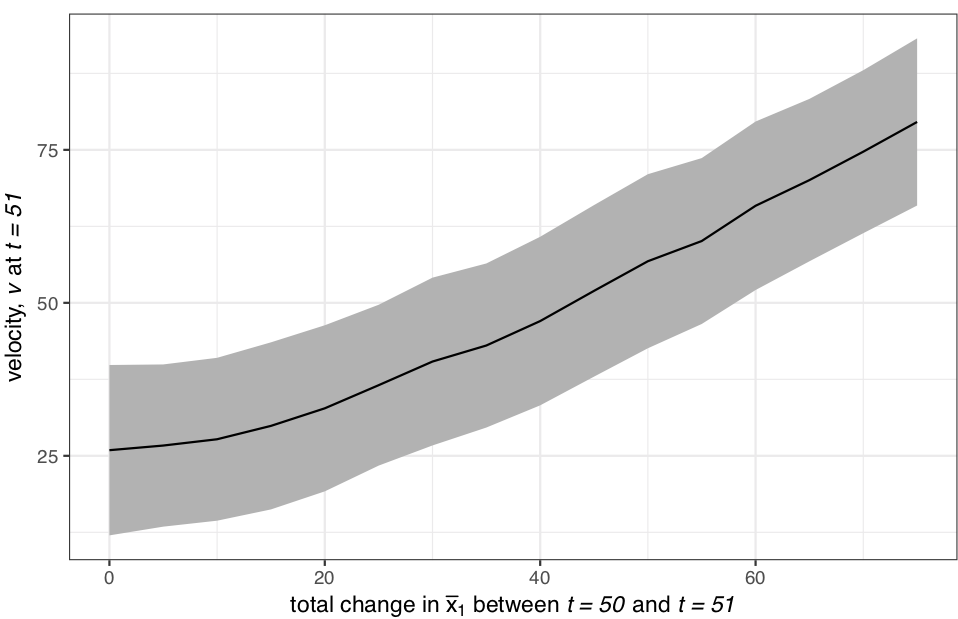
\includegraphics[width=0.85\linewidth]{/Users/jessicaburnett/Documents/GitHub/myDissertation/chapterFiles/velocity/figsCalledInDiss/simVplot2} \caption{Change in velocity ($v$) as the total change in the mean value of $\bar{x}_{2_{t=50}}$ over 10,000 simulations. A regime shift was induced at $t=50$ with constant varoance $\sigma = 5$, $\bar{x}_2 = 25$ when $t<50$,  and changes in variable mean values, $\bar{x}_2 = 50$ when $t \geq 50$, $\bar{x}_1 = 25$ when $t<50$.}\label{fig:simVplot2}
\end{figure}
\hypertarget{varying-post-shift-variance}{%
\subsubsection{Varying post-shift variance}\label{varying-post-shift-variance}}

In the previous example, variance was constant before and after the abrupt shift at \(t=50\). To determine whether the signal emitted by \(v\) at the regime shift is lost or dampened when increasing variance I varied the variance parameter, \(\sigma_1\) along the set \(W = \{1,2,3,...25 \}\). The variance for both state variables (\(x_1, x_2\)) prior to the regime shift, \(\sigma_{x_1}\) and \(\sigma_{x_2}\), was \(5\), with the change occurring in \(\sigma_{x1post}\).
\begin{figure}
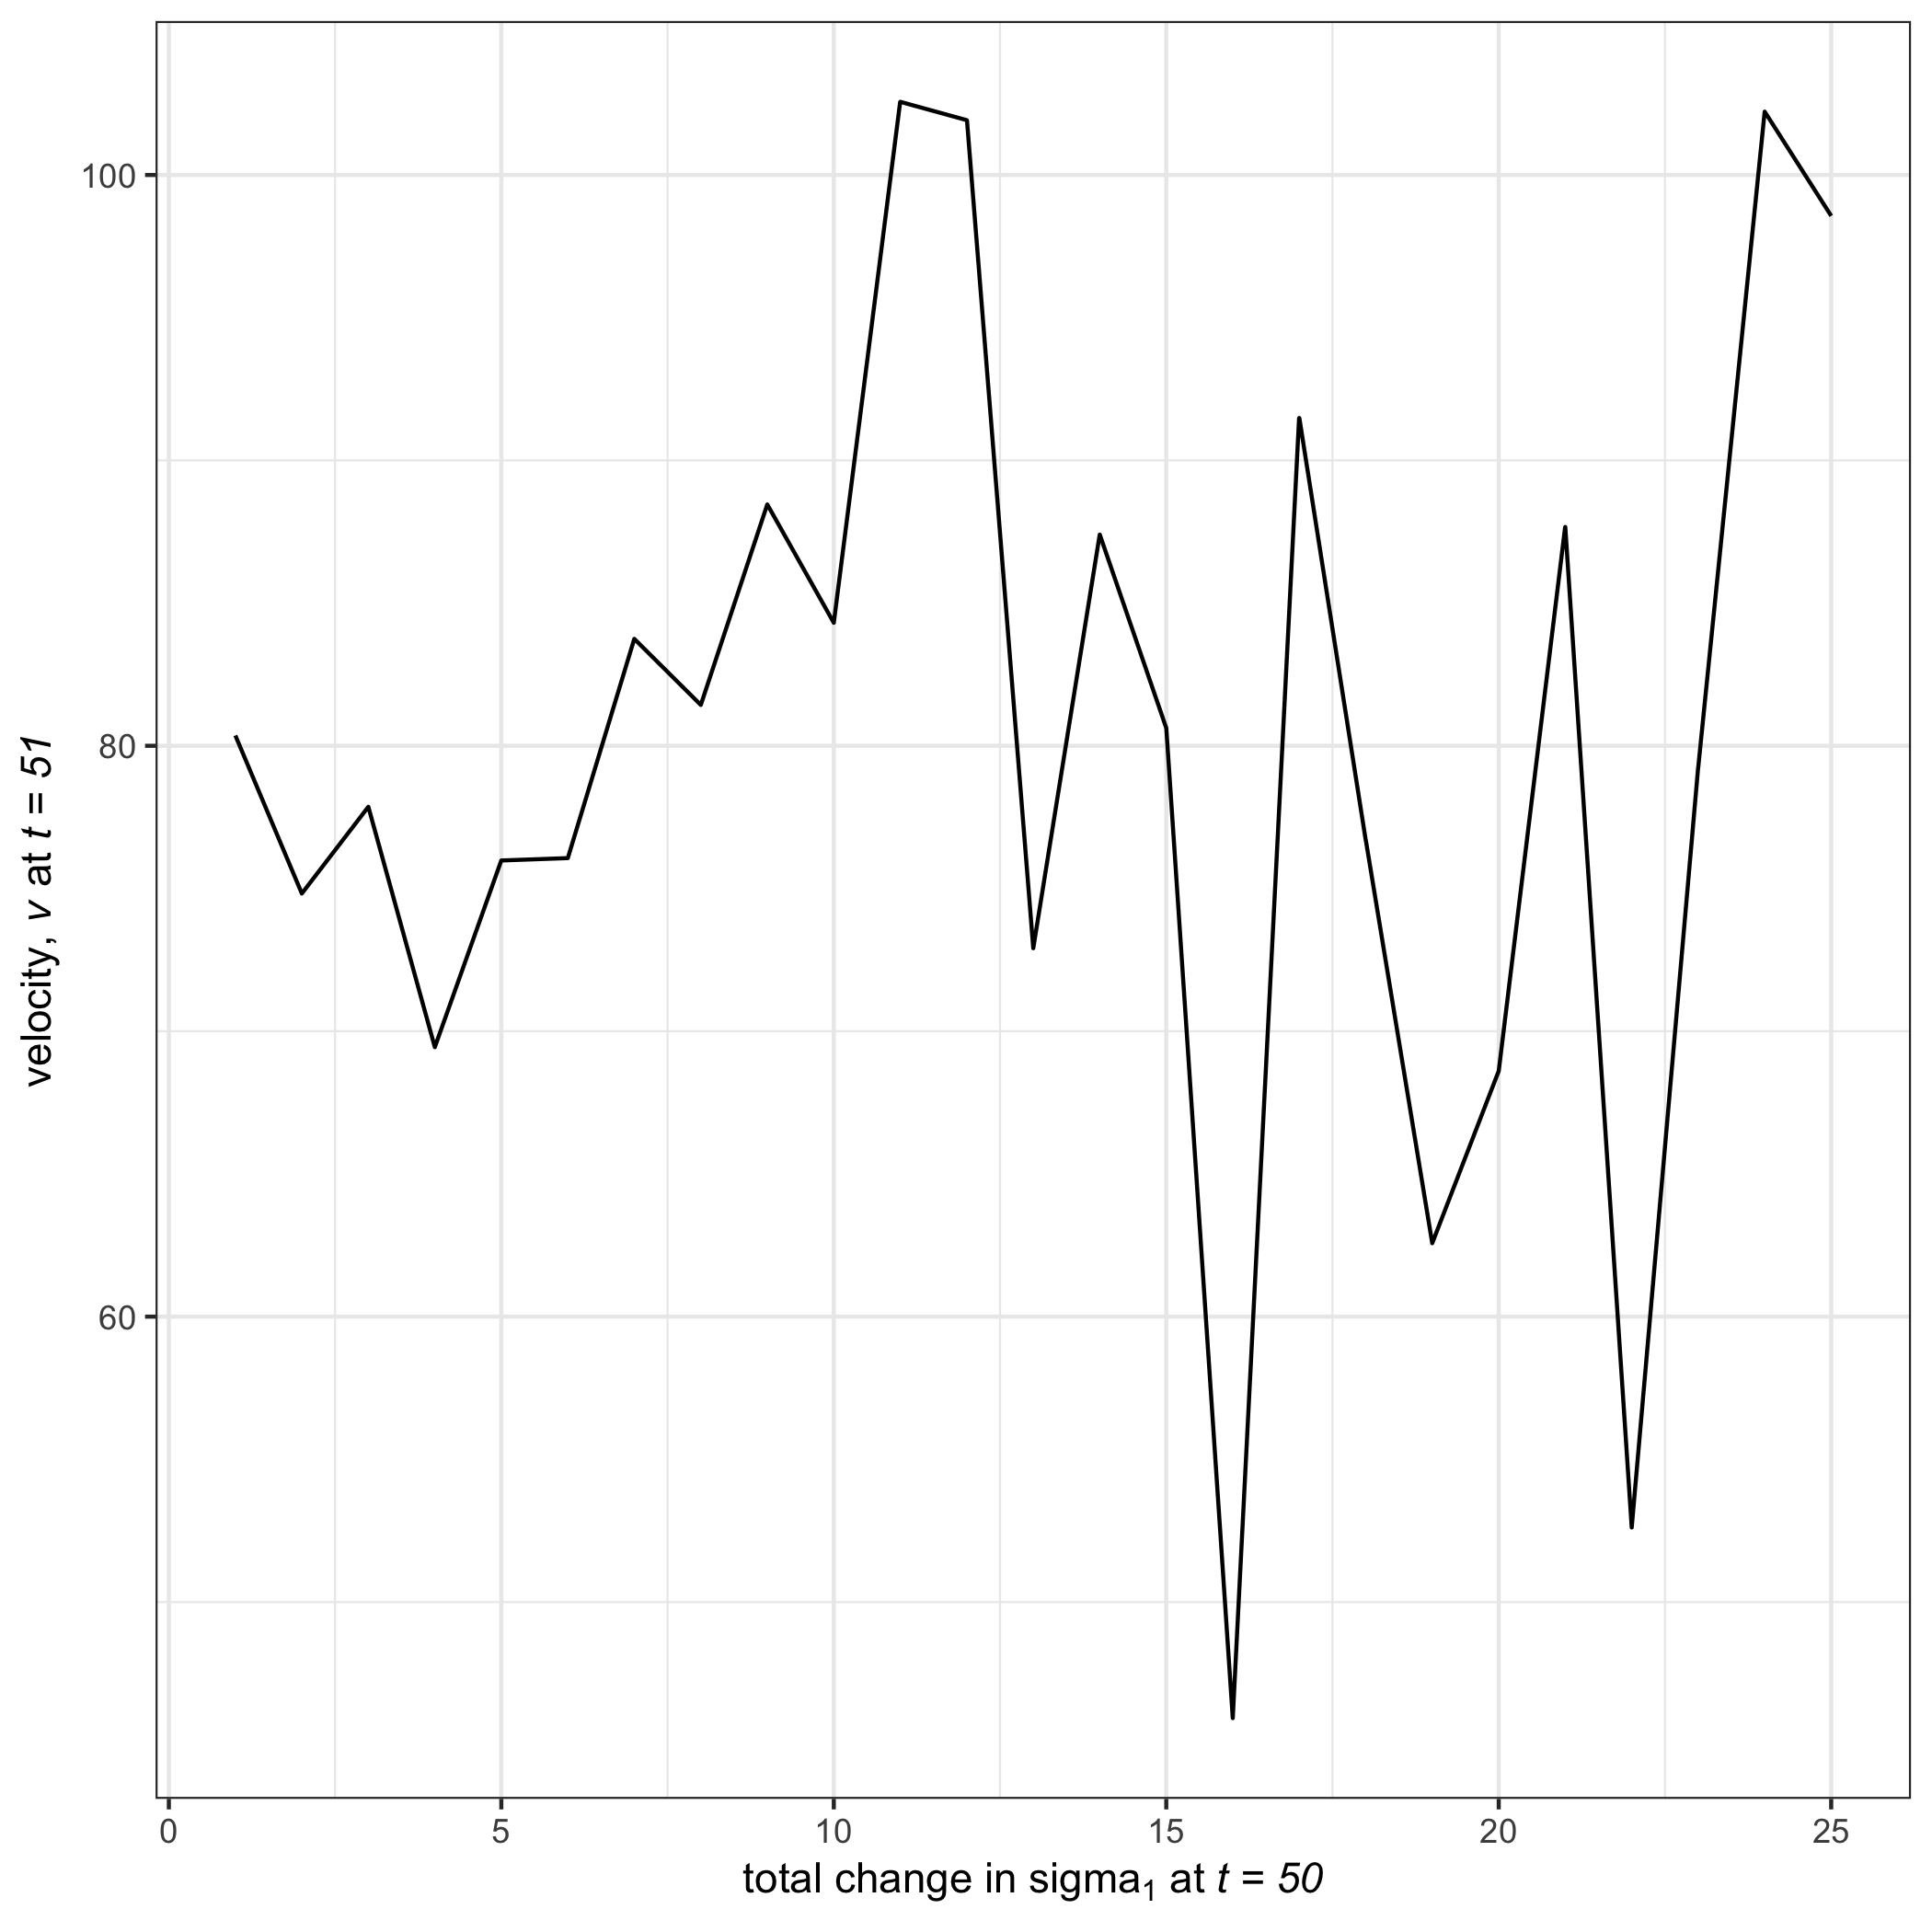
\includegraphics[width=0.85\linewidth]{/Users/jessicaburnett/Documents/GitHub/myDissertation/chapterFiles/velocity/figsCalledInDiss/simVarPlot} \caption{High variance of velocity ($v$) in a single iteration ($N_{iter}=1$, seed = 123) of simulations as we increase $\sigma_1$ at $t=50$.}\label{fig:simVarPlot}
\end{figure}
\begin{figure}
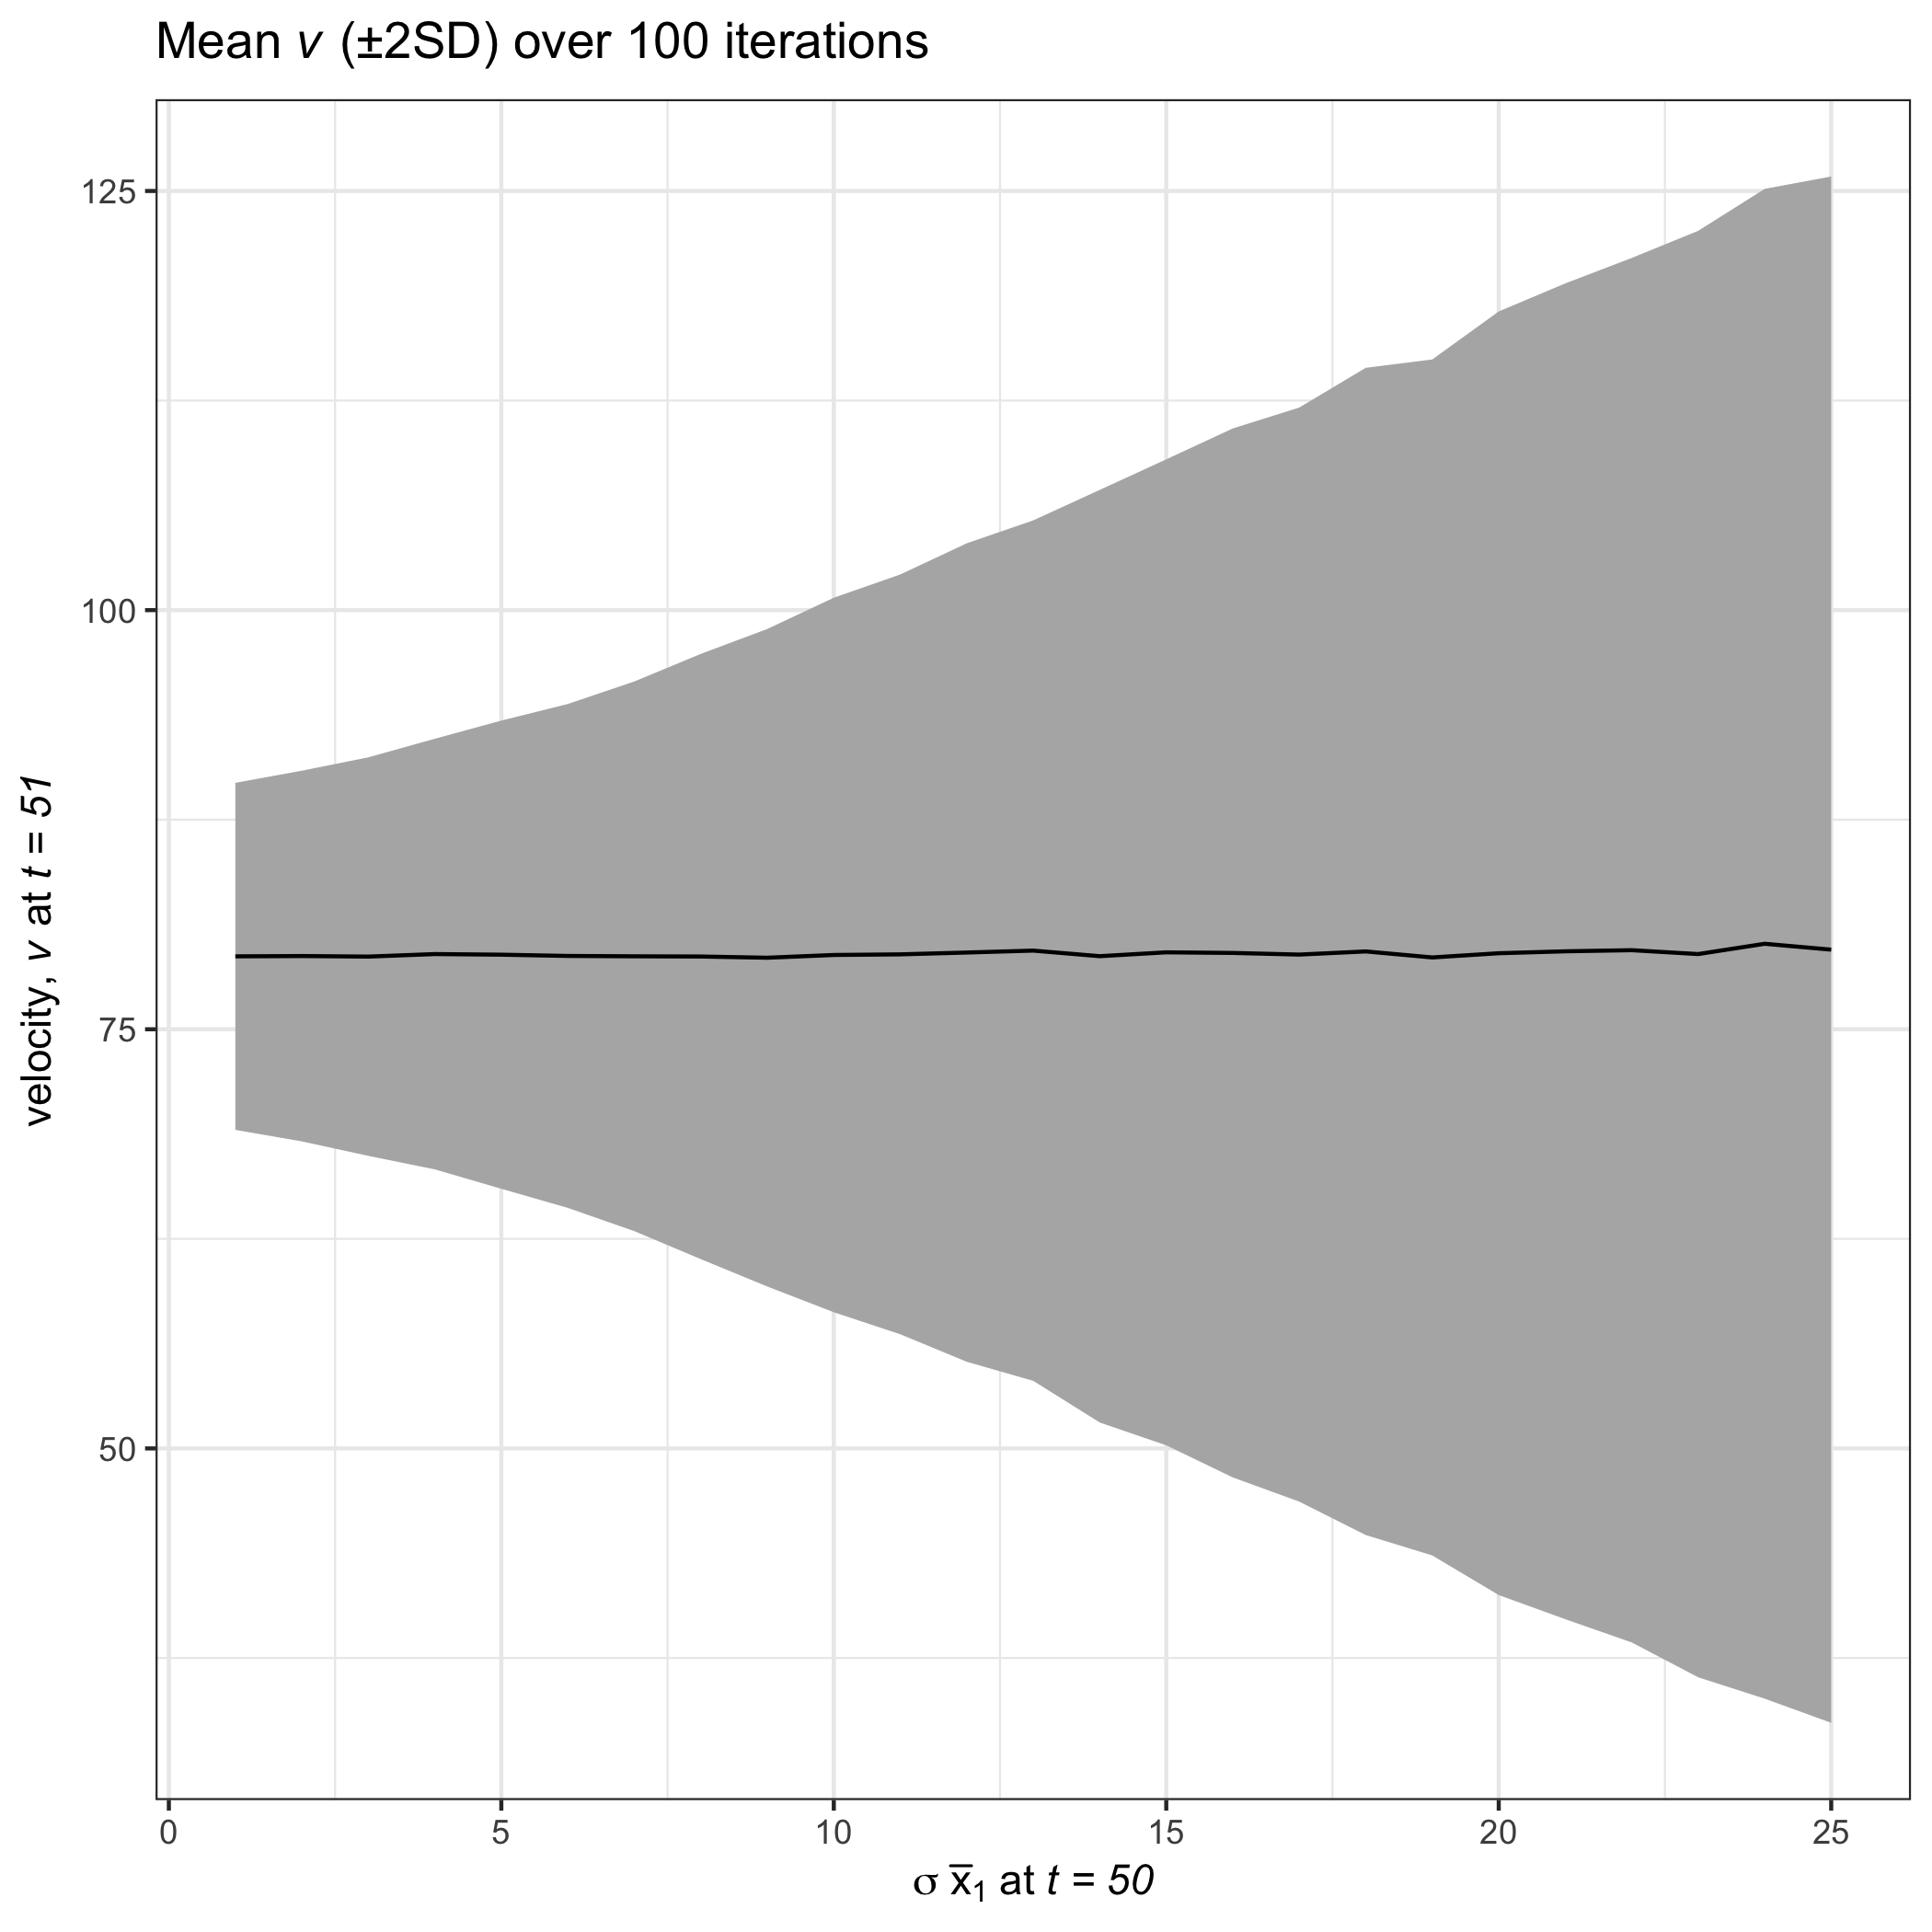
\includegraphics[width=0.85\linewidth]{/Users/jessicaburnett/Documents/GitHub/myDissertation/chapterFiles/velocity/figsCalledInDiss/simVarPlot2} \caption{Average ($\pm 2$ SD) velocity ($v$) worsens as the variance of $\bar{x}_{2_{t=50 (post)}}$ (post shift) increases. $\bar{x}_{1_{pre}} = 25$, $\bar{x}_{1_{post}} = 100$, $\bar{x}_{2_{pre}} = 25$, $\bar{x}_{2_{post}} = 50$, $\sigma_{1_{pre}} = 5$, $\sigma_{2_{pre,post}} = 5$}\label{fig:simVarPlot2}
\end{figure}
Sytem velocity \(v\) appears senstive to increases in the variance at the point of the regime shift (Figs. \ref{fig:simVarplot}, \ref{fig:simVarplot2}). Again, because velocity is a function of the total change in the state variables, the variability of \(v\) will increase with both \(mu\) and \(\sigma\) (Fig. \ref{fig:simVarplot2}). Further, it is unsurpirsing that \(v\) exhibits sensitivity to changes in \(\sigma_{post}\) because, without prior smoothing of the data, the tangential speed of a `noisy' variable will always be noisy itself (see Figs. \ref{velocitySysEx1}, \ref{velocitySysEx2}, \ref{velocitySysEx3}, \ref{velocitySysEx4}).

\hypertarget{smoothing-the-data-prior-to-calculating-v}{%
\subsubsection{\texorpdfstring{Smoothing the data prior to calculating \emph{v}}{Smoothing the data prior to calculating v}}\label{smoothing-the-data-prior-to-calculating-v}}

To determine whether process or observational noise influences the signal in \(v\), I used linear approximation techniques to smooth the data prior to calculating the derivatives. I used the function \emph{stats::approx} which linearaly interpolates the original data, \(x_1\) and \(x_2\), to regularly-spaced time points along the set \(t=\{1:100\}\). I then calculated \(v\) as described in (Eqs. \eqref{eq:diffX}:\eqref{eq:velocity}). Increasing the number of points (\(t\)) at which the original state variables were smoothed (i.e., \(t\)) did not influence the amount of noise surrounding the signal of the regime shift (at \(t=50\)) in system velocity, \(v\) (Fig. \ref{fig:smoothV}).
\begin{figure}
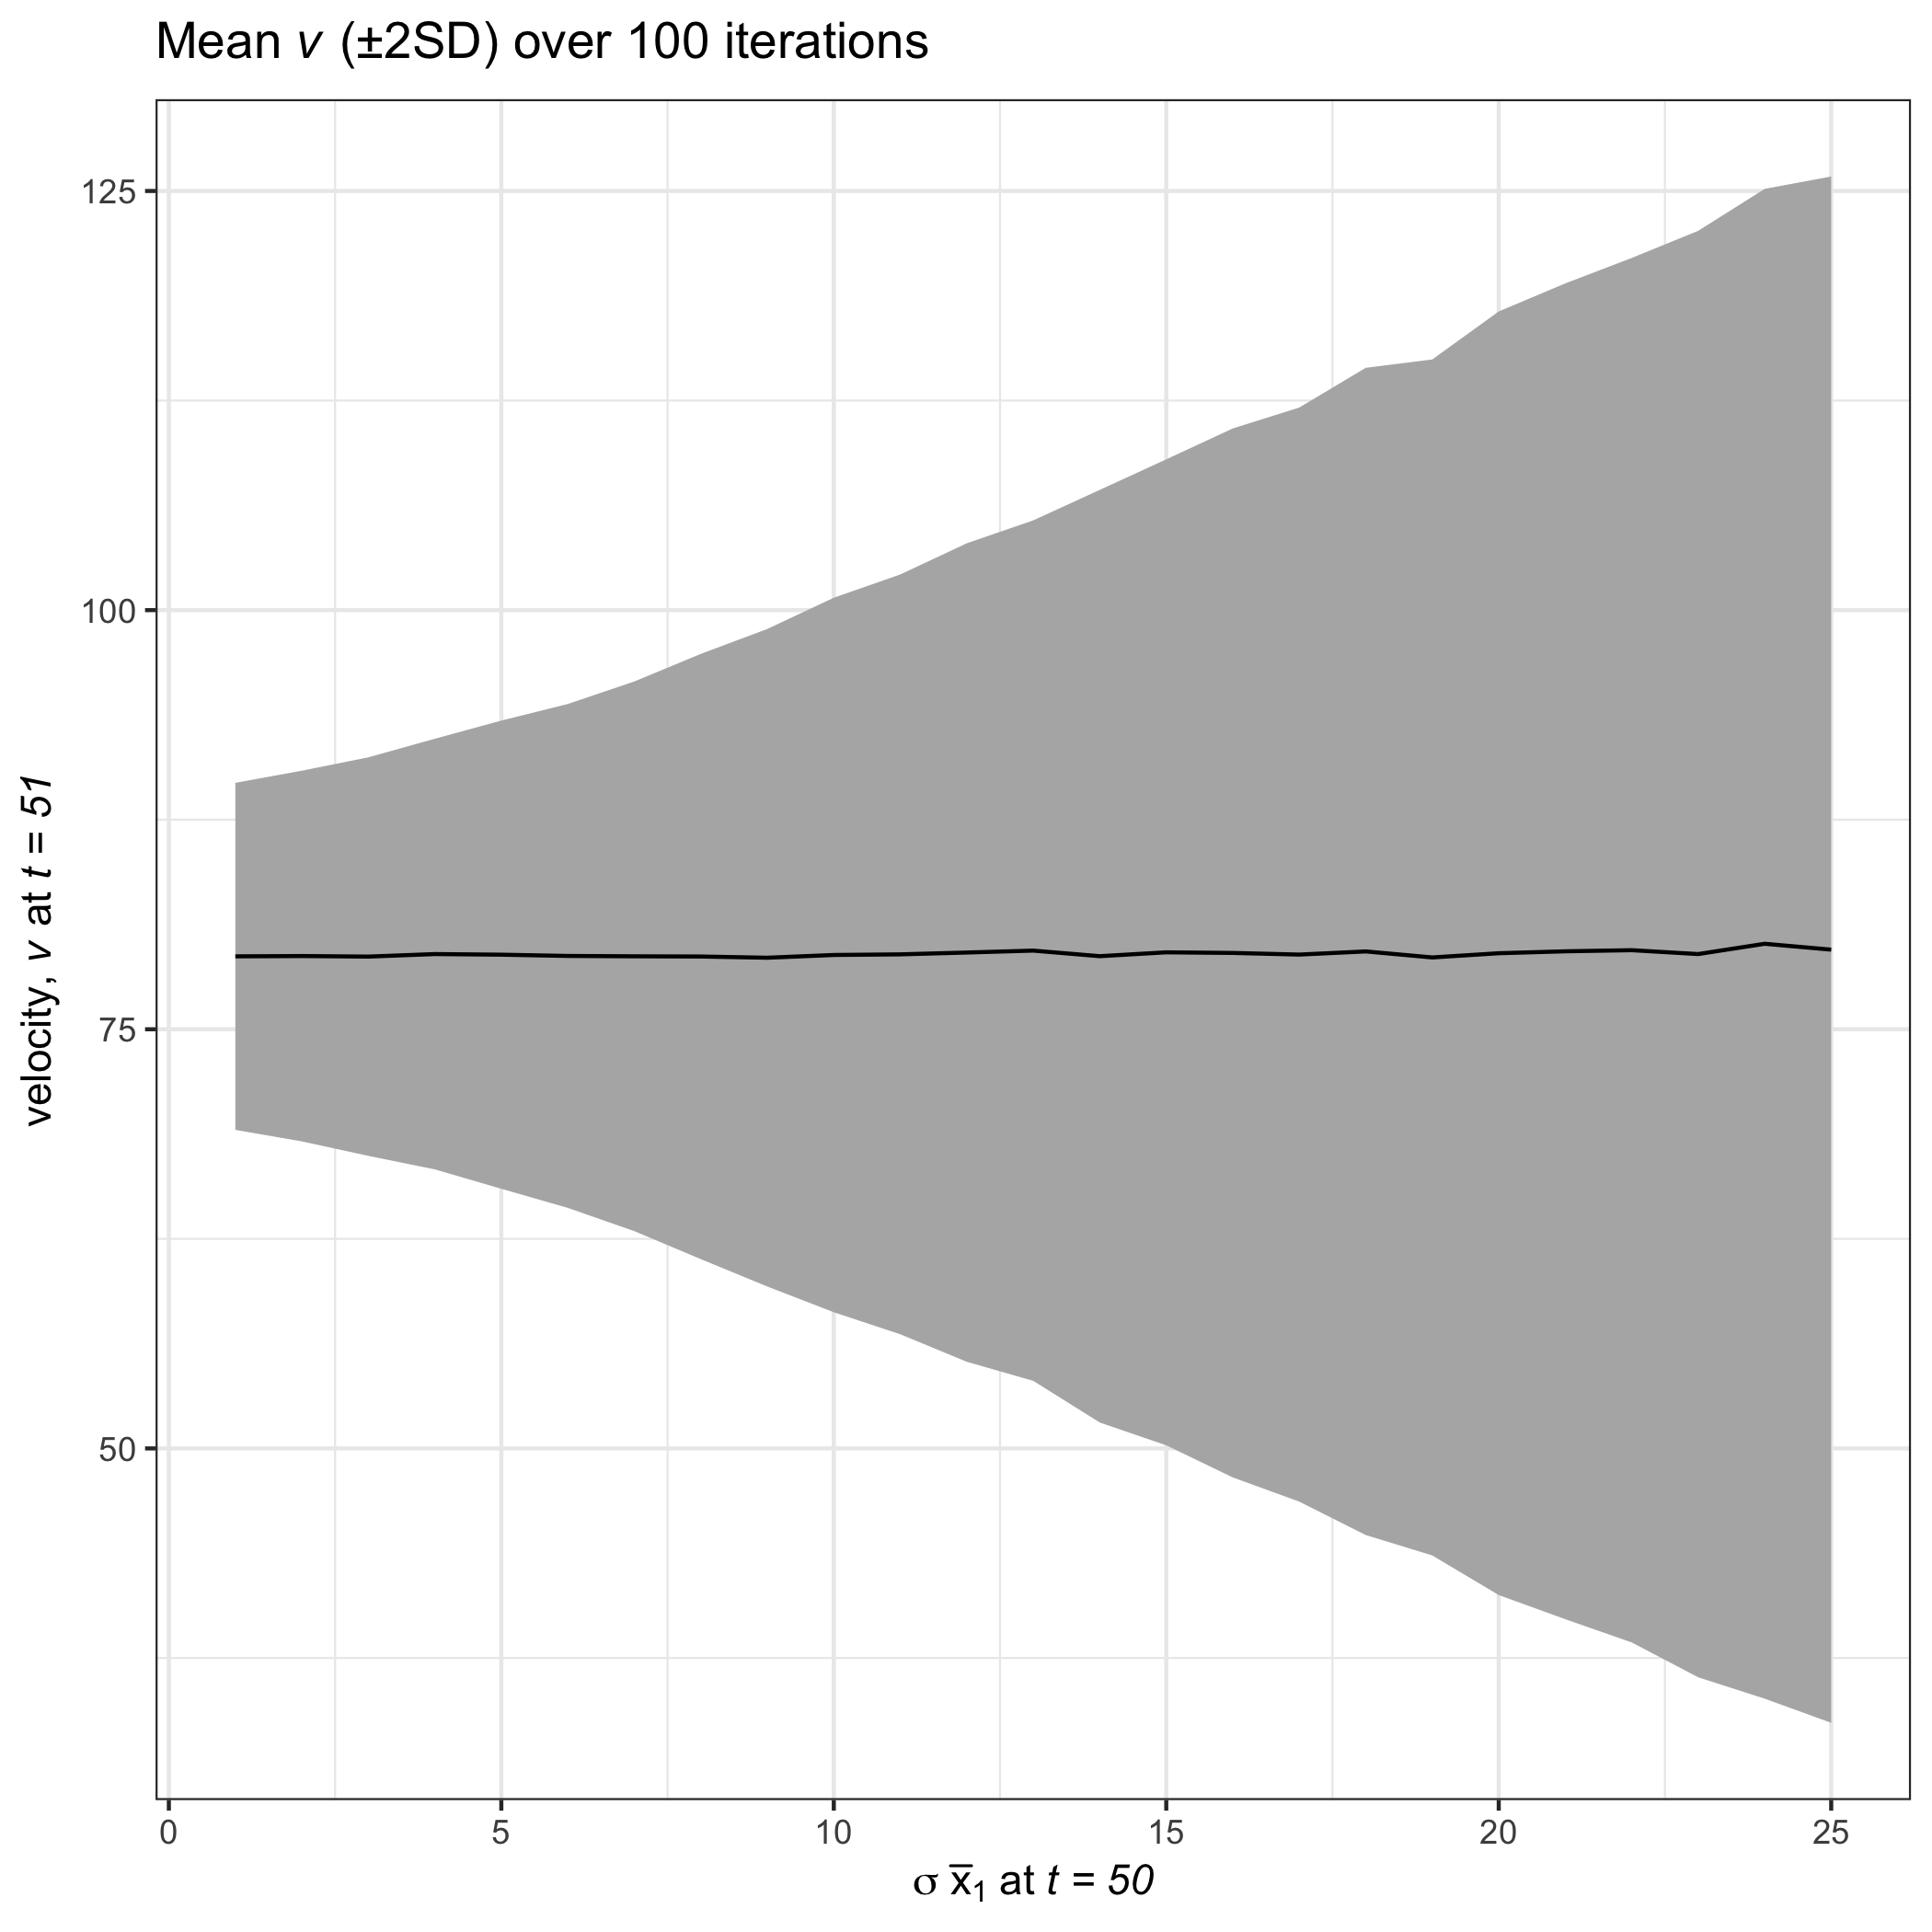
\includegraphics[width=0.85\linewidth]{/Users/jessicaburnett/Documents/GitHub/myDissertation/chapterFiles/velocity/figsCalledInDiss/smoothV} \caption{The noise in system velocity ($v$) is not obviously reduced in this system as the original data ($x_1$, $x_2$) is increasingly smoothed.}\label{fig:smoothV}
\end{figure}
\hypertarget{velocity-performance-under-a-smooth-transition}{%
\section{Velocity performance under a smooth transition}\label{velocity-performance-under-a-smooth-transition}}

In the previous section I presented expectations for velocity signals under a discontinuous transition in a discrete-time system. Given velocity is a measure of the rate of a change in a system and the range of transition speeds ecological systems exhibit (e.g., slow driver-response or threshold dynamics), it is important to understand if and when the velocity signal is dampened under varying degrees of transition speeds. In this section I use a similar toy system, to demonstrate the expectations of velocity under a smooth shift and under varying degrees of rapidity.

Although the data constructed in this section are similar to that used in the previous section in that we are manipulating the mean and variance of two state variables before and/or after an abrupt shift, this section introduces a component of process noise into the shift itself. This is important because the derivative of a nearly discontinuous function is infinite. Although we are interested in identifying rapid shifts in systems, velocity will appraoch infinity as the rate of change in the shift increases and the sampling intervals decrease. In other words, if the system exhibits turnover in e.g.~\(25\%\) of the state variables, we expect the value of velocity to be similar to that of a turnover in e.g.~\(75\%\) of the variables. Removing the possibility of infinite values provides more relative measures within the community time series.

\hypertarget{generating-the-data}{%
\subsection{Generating the data}\label{generating-the-data}}

Here we consider a two-variable system over the time interval \([1,100]\) with state variables \(x_1\) and \(x_2\) which exhibits abrupt shifts in mean and/or variance of one or both variables at time \(t=50\). I generated species observations for the true process and the true process with process variability. The true process data were created using the paramters for \(\mu\) and \(\sigma\) for each of the conditions in described in Table \ref{tab:sysParams} (random seed in Program R was 12345).
\begin{table}[t]

\caption{\label{tab:sysParams}Conditions for generating various scenarios of the hyperbolic tangent-induced abrupt change. $\sigma_i$ represents the standard deviation of $\mu_{x_i}$ as the percent of $\mu_{x_i}$, $\mu_{x_i}$ is the mean of the state variable, $x_i$, and pre and post represent the periods before and after the regime shift at $t=50$, respectively.}
\centering
\begin{tabular}{lllllllll}
\toprule
conditions & $\sigma_{x_{1_{pre}}}$ & $\sigma_{x_{1_{post}}}$ & $\sigma_{x_{2_{pre}}}$ & $\sigma_{x_{2_{post}}}$ & $\mu_{x_{1_{pre}}}$ & $\mu_{x_{1_{post}}}$ & $\mu_{x_{2_{pre}}}$ & $\mu_{x_{2_{post}}}$\\
\midrule
$\mu_{x_1}$, $\mu_{x_2}$, $\sigma_{x_1}$, $\sigma_{x_2}$ & 0.05 & 0.10 & 0.05 & 0.10 & 10 & 55 & 15 & 44\\
$\mu_{x_1}$, $\sigma_{x_1}$ & 0.05 & 0.10 & 0.05 & 0.05 & 10 & 55 & 15 & 15\\
$\mu_{x_1}$, $\mu_{x_2}$ & 0.05 & 0.05 & 0.05 & 0.05 & 10 & 55 & 15 & 44\\
$\mu_{x_1}$ & 0.05 & 0.05 & 0.05 & 0.05 & 10 & 55 & 15 & 15\\
$\sigma_{x_1}$, $\sigma_{x_2}$ & 0.05 & 0.10 & 0.05 & 0.10 & 10 & 10 & 15 & 15\\
\addlinespace
$\sigma_{x_1}$ & 0.05 & 0.10 & 0.05 & 0.05 & 10 & 10 & 15 & 15\\
\bottomrule
\end{tabular}
\end{table}
\hypertarget{true-process-model}{%
\subsubsection{True process model}\label{true-process-model}}

Data were generated from a normal distribution and an abrupt shift in the mean was incorporated using a hyperbolic tangent function. The true process for each state variable, \(x_i\), was generated from Eq. (\eqref{eq:true} (Fig. \ref{fig:trueObsEx})):
\begin{equation}
\mu_{xipre}\sim Normal(\mu_{xipre},\sigma_{xipre}) \\ 
\mu_{xipost} \sim Normal(\mu_{xipre}, \sigma{xipost}) \\ 
\mu_{x_i}(t) = \mu_x{_ipre}  - 0.5(\mu_x{_ipre}-\mu_{xipost})(\tanh(\alpha (t-t_{shift}))+1) \\ f
\label{eq:true}
\end{equation}
where \(\mu_{x_i}(t)\) is the mean value of \(x_i\) at time \(t\) and \emph{pre} and \emph{post} are the periods before and after the abrupt shift (\(t_{shift}\)), respectively. The parameter \(\alpha\) in Eq. \eqref{eq:true} controls for the rate of change at the point of the abrupt change, \(t_{shift}\), where higher values of \(\alpha\) correspond with a higher slope at \(t_{shift}\). I simulated a single iteration (dataset) for various conditions of changing \(\mu_{xi}\) and \(\sigma_{xi}\) (see Table \ref{tab:sysParams}), for two state variables \(x_1\ \&\ x_2\) at intervals of \(t=1\) along the temporal interval \(t=[1,100]\).
\begin{figure}
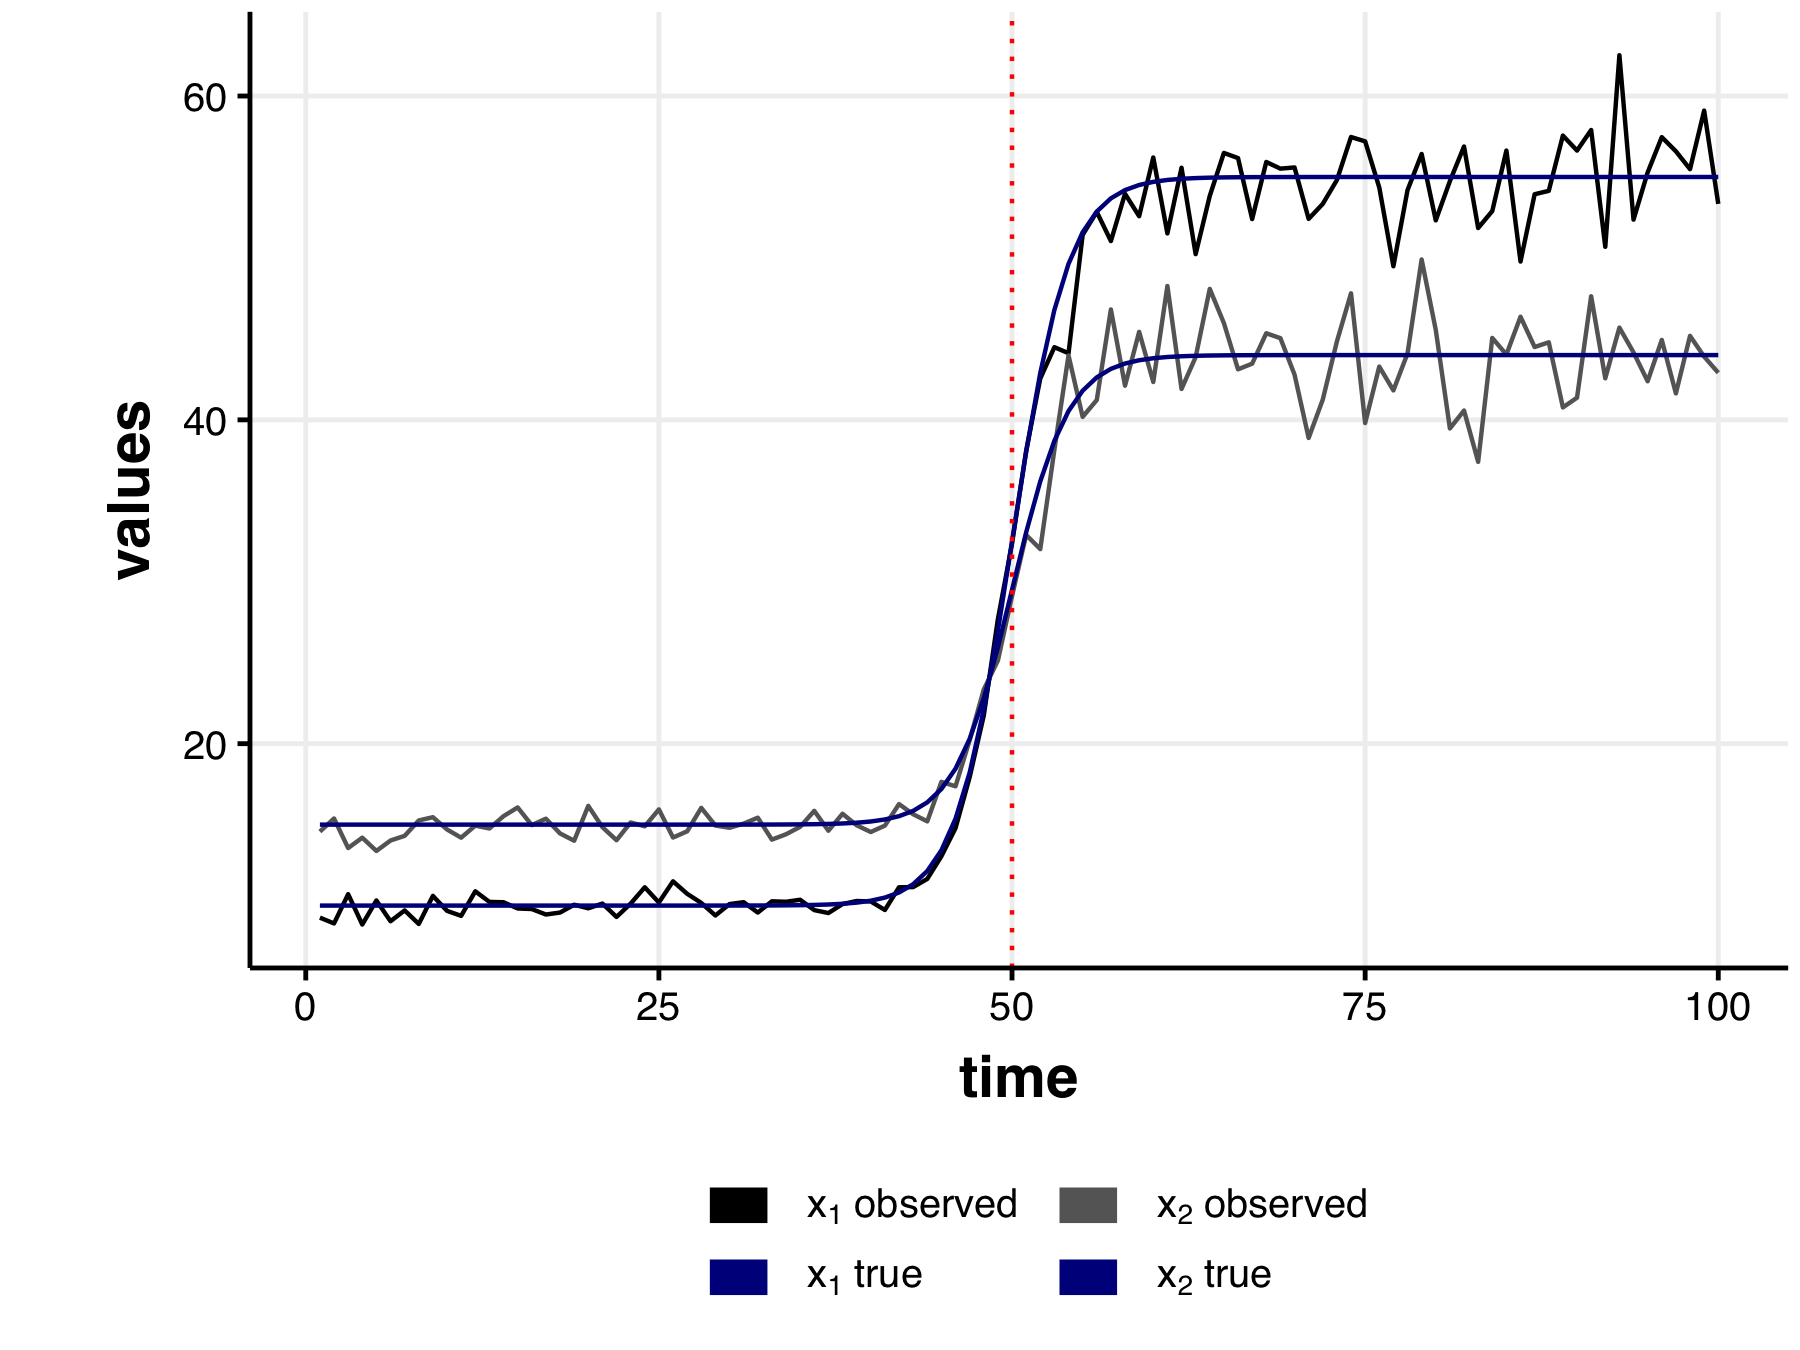
\includegraphics[width=0.85\linewidth]{/Users/jessicaburnett/Documents/GitHub/myDissertation/chapterFiles/velocity/figsCalledInDiss/changeMuBoth_tanhAlpha025-05tvdiffAlpha-1000iter_origDat} \caption{An example of the data generated by the true process model. In this example the mean values ($\mu_{xi}$), but not the percent standard deviation ($\sigma_{xi}$), are varied before and after the transition point. The observed data are plotted against the true-process model for each state variable, $x_i$. Panels represent different degrees of the smoothing parameter, $\alpha$ (top: $\alpha=0.25$, bottom:$\alpha=1.00$).}\label{fig:trueObsEx}
\end{figure}
\begin{figure}
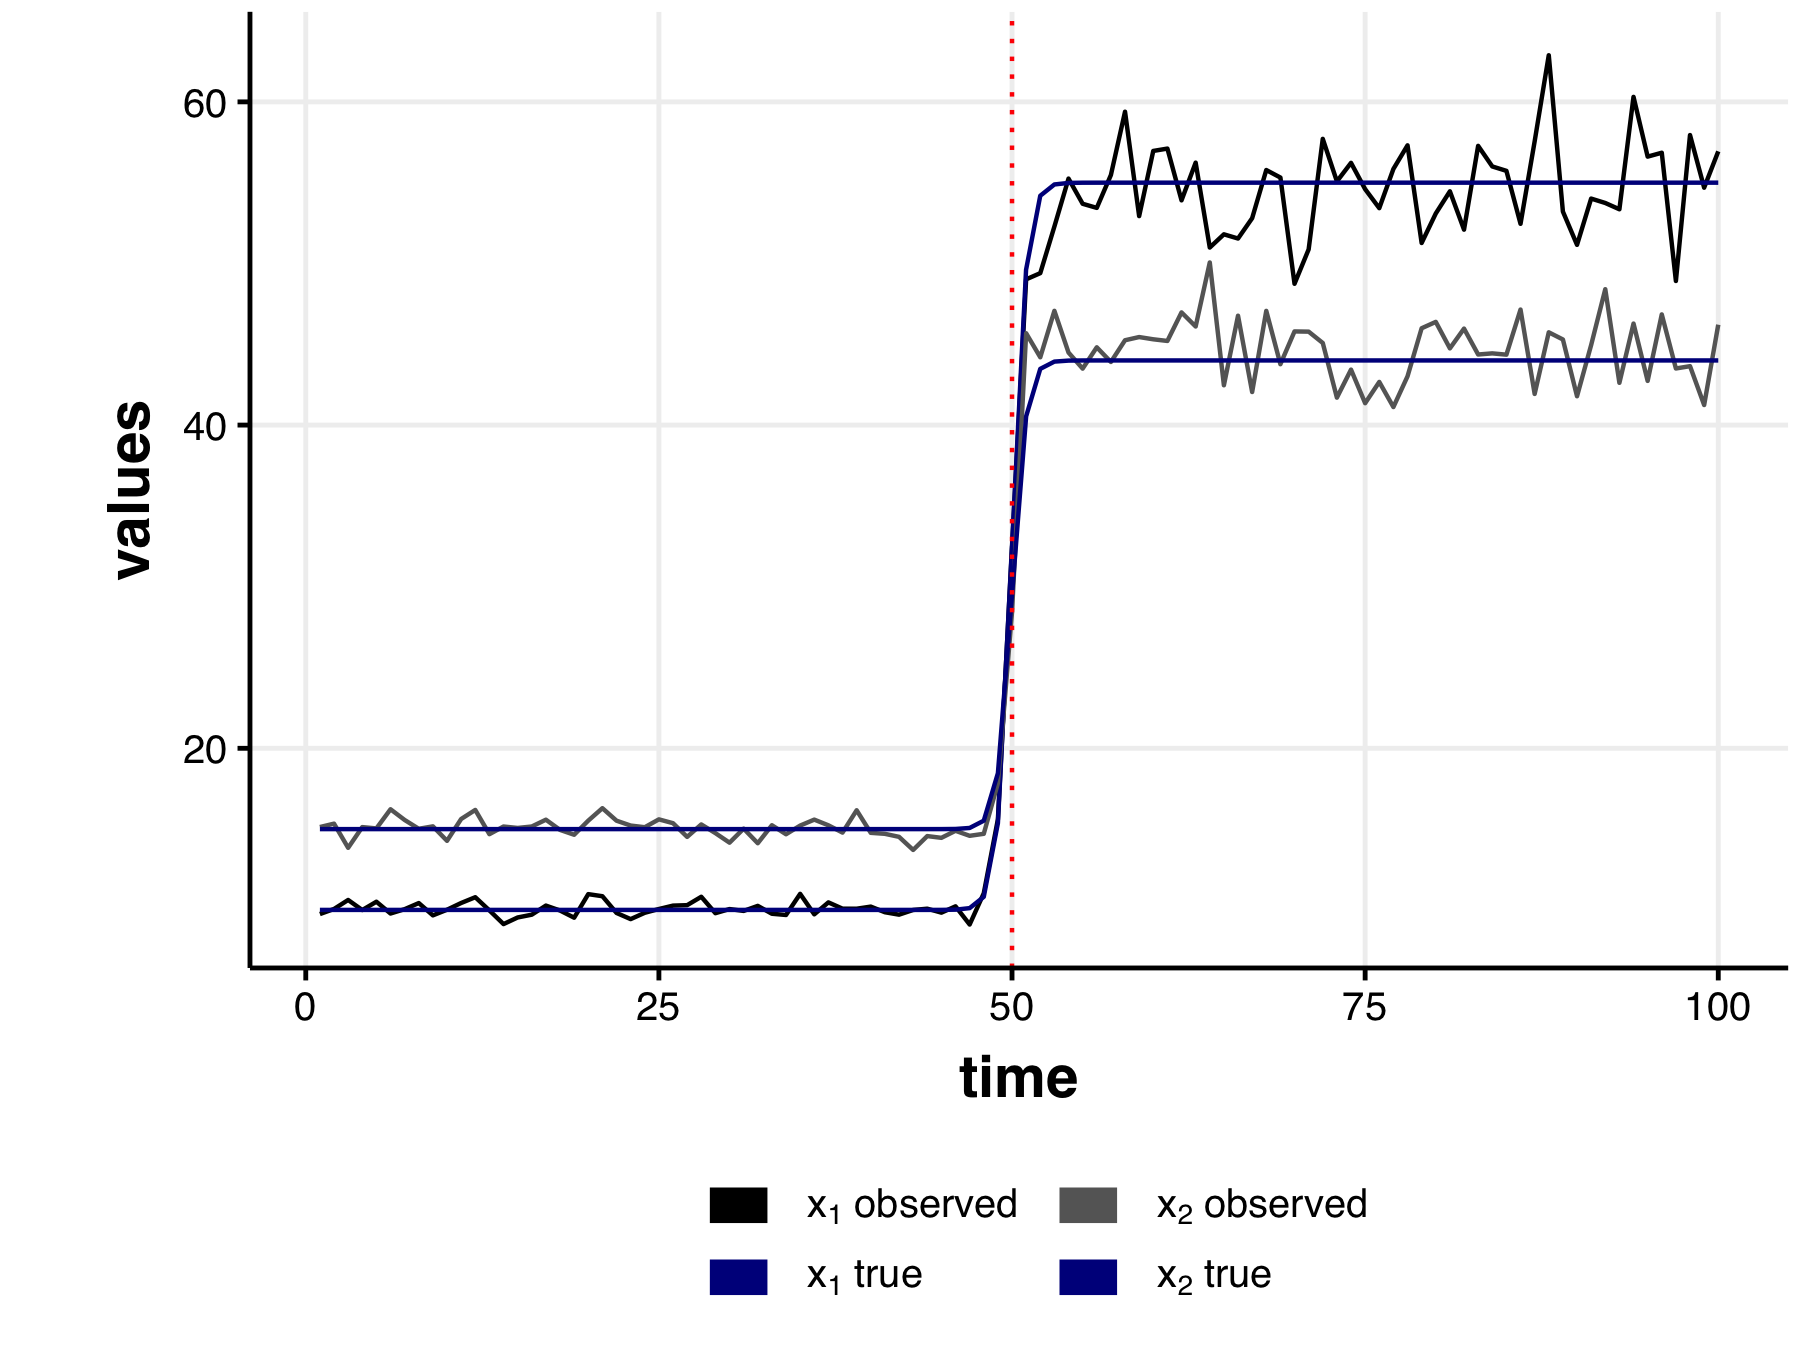
\includegraphics[width=0.85\linewidth]{/Users/jessicaburnett/Documents/GitHub/myDissertation/chapterFiles/velocity/figsCalledInDiss/changeMuBoth_tanhAlpha1-100tvdiffAlpha-1000iter_origDat} \caption{An example of the data generated by the true process model. In this example the mean values ($\mu_{xi}$), but not the percent standard deviation ($\sigma_{xi}$), are varied before and after the transition point. The observed data are plotted against the true-process model for each state variable, $x_i$. Panels represent different degrees of the smoothing parameter, $\alpha$ (top: $\alpha=0.25$, bottom:$\alpha=1.00$).}\label{fig:trueObsEx}
\end{figure}
\hypertarget{observed-process-data}{%
\subsubsection{Observed process data}\label{observed-process-data}}

I generated observations by imputing noise into the true process model (Eq. \eqref{eq:true}) through random sampling of \(\sigma_x{_i}\) from a normal distribution (Eq. \eqref{eq:observed}; Fig. \ref{fig:trueObsEx}):
\begin{equation}
\mu_{xipre}\sim Normal(\mu_{xipre},\sigma_{xipre}) \\ 
\sigma_{xipre} \sim Normal(0,\sigma_{Xipre}\mu_{Xipre}) \\
\mu_{xipost} \sim Normal(\mu_{ipost},\sigma_{ipost}) \\ 
\sigma_{xipost} \sim Normal(0,\sigma_{Xipost}\mu_{xipost}) \\
\mu_{xi}(t) = \mu_x{_ipre}  - 0.5(\mu_{xipre}-\mu_{xipost})(\tanh(\alpha (t-t_{shift}))+1) \\
\label{eq:observed}
\end{equation}
where \(\sigma_{xi}\) is the observed error around \(\mu_{xi}\), and \(\sigma_{Xi}\) is \(X\%\) of \(\mu_{xi}\) under various sampling conditions (as described in Table \ref{tab:sysParams}). I generated the error as a percent of the mean as this scaling relationship is commonly observed in ecological data (Taylor, 1961).

\hypertarget{evaluating-velocity-performance-under-conditions-of-changing-means-andor-variance}{%
\subsection{Evaluating velocity performance under conditions of changing means and/or variance}\label{evaluating-velocity-performance-under-conditions-of-changing-means-andor-variance}}

I simulated a single dataset (R seed 12345) by randomly drawing a single realisation (observed data) of the hyperbolic tangent process model with additive process noise (Eq. \eqref{eq:observed}). I then calculated the distance travelled, \(s\), and the velocity of the distance travelled, \(v\) (also referred to as \(\frac{ds}{dt}\)) using first differences. The first differences approach is a simple alternative to numerical integration tecniques, requiring only simple algebraic techniques. This method is ideal for discrete time data, or where computational power woudl not suffice for numerical integration. When using the first differences method, however, \(v\) will demonstrate high variability, depending on the amount of time between samples (i.e.~as the intervals of \(t-t+1\) increase).

I also calculated \(v\) using a numerical integration method for non-smooth, noisy data, called total variation regularized differentiation (Chartrand, 2011). I used the R package \texttt{tvdiff} (Price \& Burnett, 2019) to perform numerically integrate the distance travelled, \(s\). The regularized differentiation method in this package (function \texttt{tvRegDiff}; descried fully in Chartrand, 2011) provides a numerical solution for calculating non-noisy derivatives of noisy, non-smooth data. Using this smooth-derivative estimation technique may be an ideal supplement to the velocity method in cases where process and observational error generate noisy observational data. Although not possible in most ecological systems data, here we can compare the fit of the smooth-derivative to the derivative of the true process, allowing us to determine the usefulness of calculating a smooth-derivative. There are two tuning paramters required to be chosen by the analyst when implementing the total-variation regularized differentiation, each of which influence the amount of noise smoothed out in the resulting derivative: \(\alpha\) and the number of iterations. I implemented this numerical differentiation over 1,000 iterations, and selected \(\alpha\) by comparing the antidifferentiated distance travelled, \(s\), to the true process values of \(s\) (e.g., see Figure \ref{fig:antiDiffComp}). For most conditions and smoothness I found the tuning parameter for \texttt{tvdiff} \(\alpha=0.50\) provided a good fit of \(s\) (Fig. \ref{fig:antiDiffComp}), however, when the hyperbolic tangent smoothing paramter, \(\alpha\) was low (i.e.~\(\alpha_{tanh}=0.25\)) higher values of \(\alpha_{tvdiff}\) yielded more abrupt changes in the derivative.
\begin{figure}
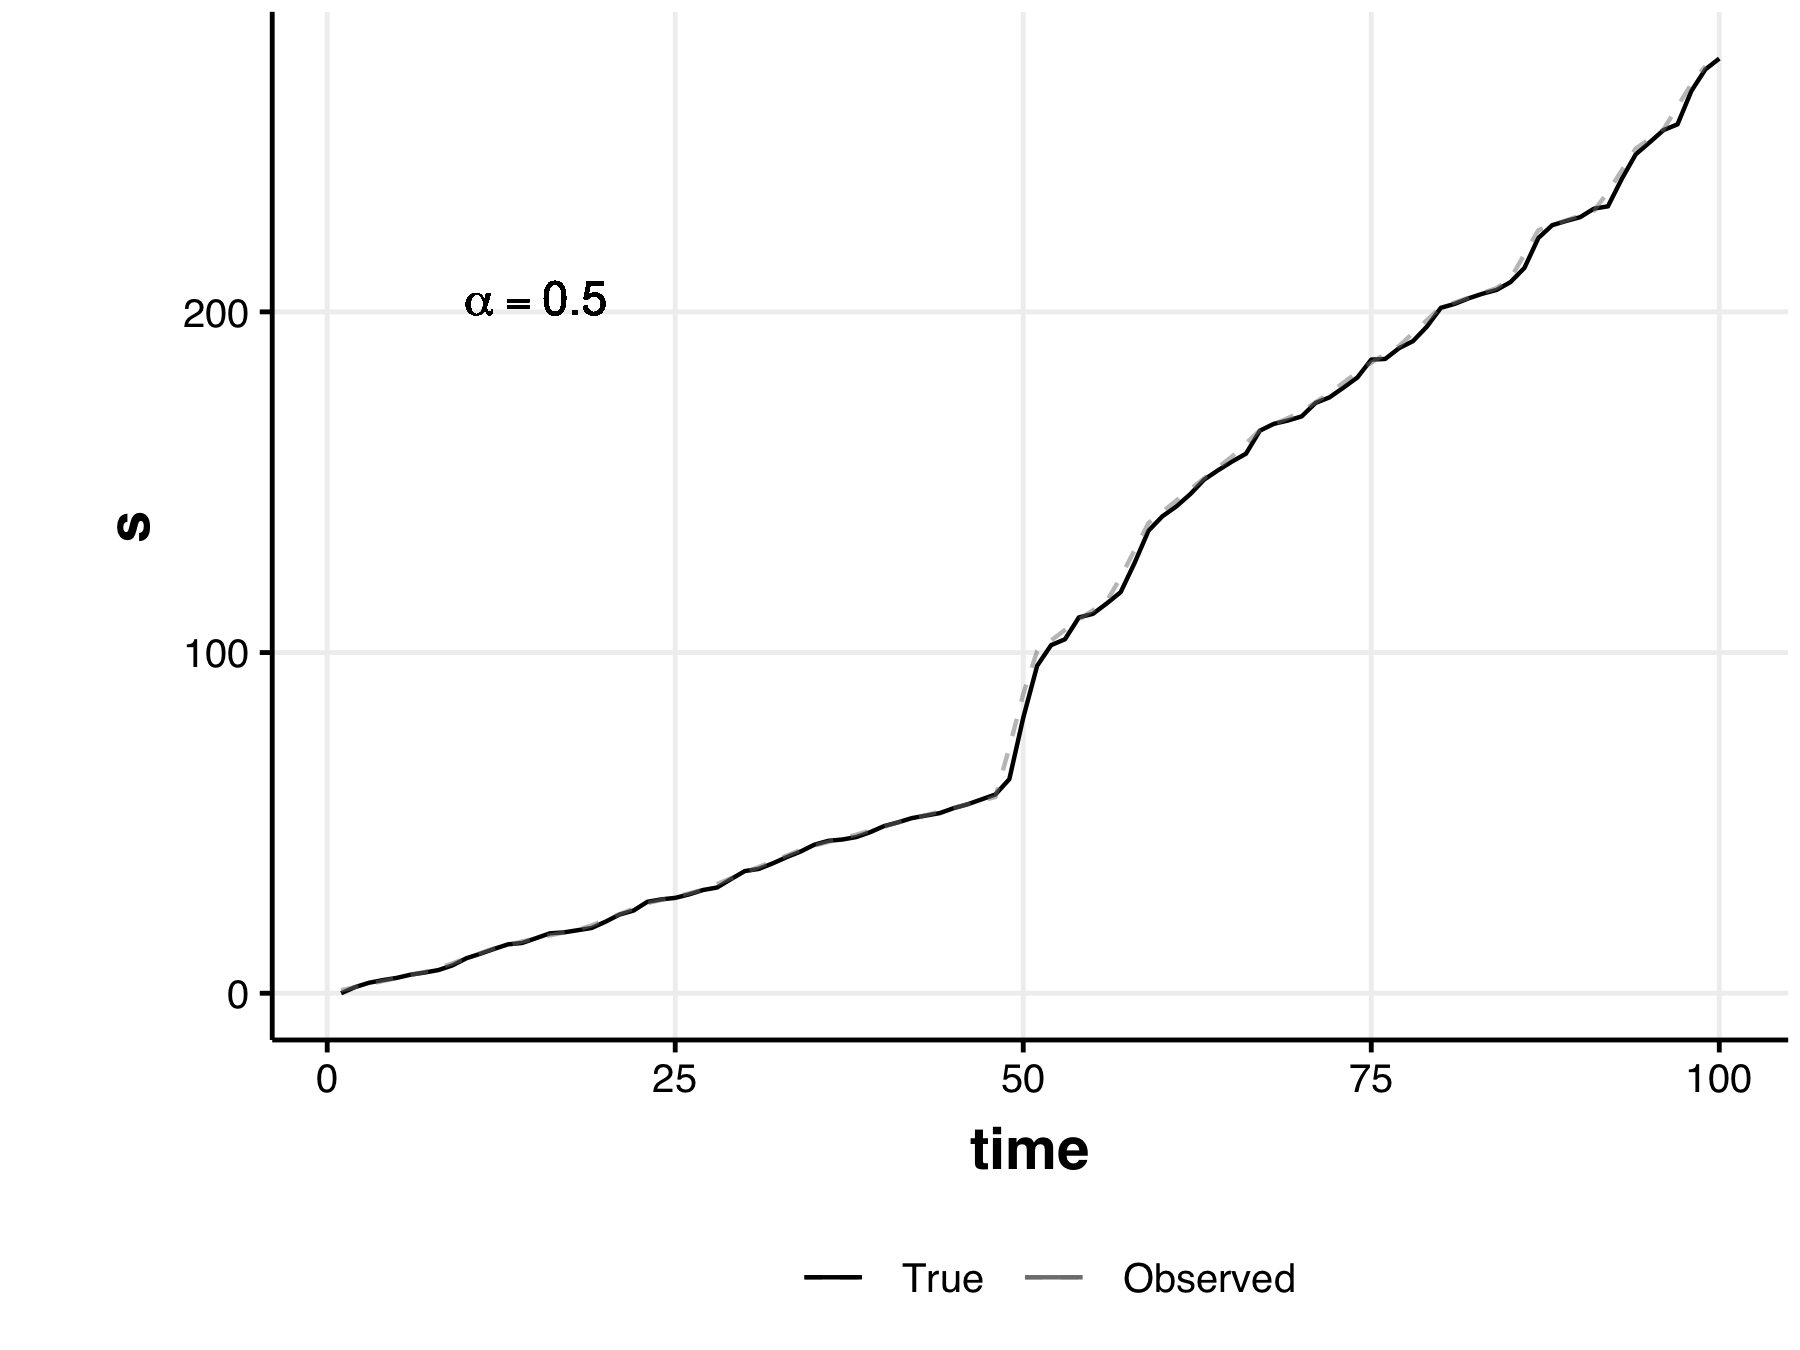
\includegraphics[width=0.33\linewidth]{/Users/jessicaburnett/Documents/GitHub/myDissertation//chapterFiles/velocity/figsCalledInDiss/compareTvdiff_s_changeMuX1_tanhAlpha1-05tvdiffAlpha-1000iter} \caption{Comparison of the antidifferentiated values ('observed') of the distance travelled, $s$, to the true process values of $s$ ('true) provides a method for identifying the best values of the smooothing parameter, $\alpha$. Under most conditions $\alpha \ll$ sufficed. Here, we compare the true and antidifferentiated values of $s$ under the condition of changing $\mu_{x1}$ when the hyperbolic tangent function is most rapid ($\alpha_{tanh}=1$) for the `tvdiff` alpha values of: $\alpha=0.50$ (top), $\alpha=1$ (middle), and $\alpha=10$ (bottom). Notice that the antidifferentiated $s$ (observed) is increasingly smoothed as $\alpha$ increases.}\label{fig:antiDiffComp}
\end{figure}
\begin{figure}
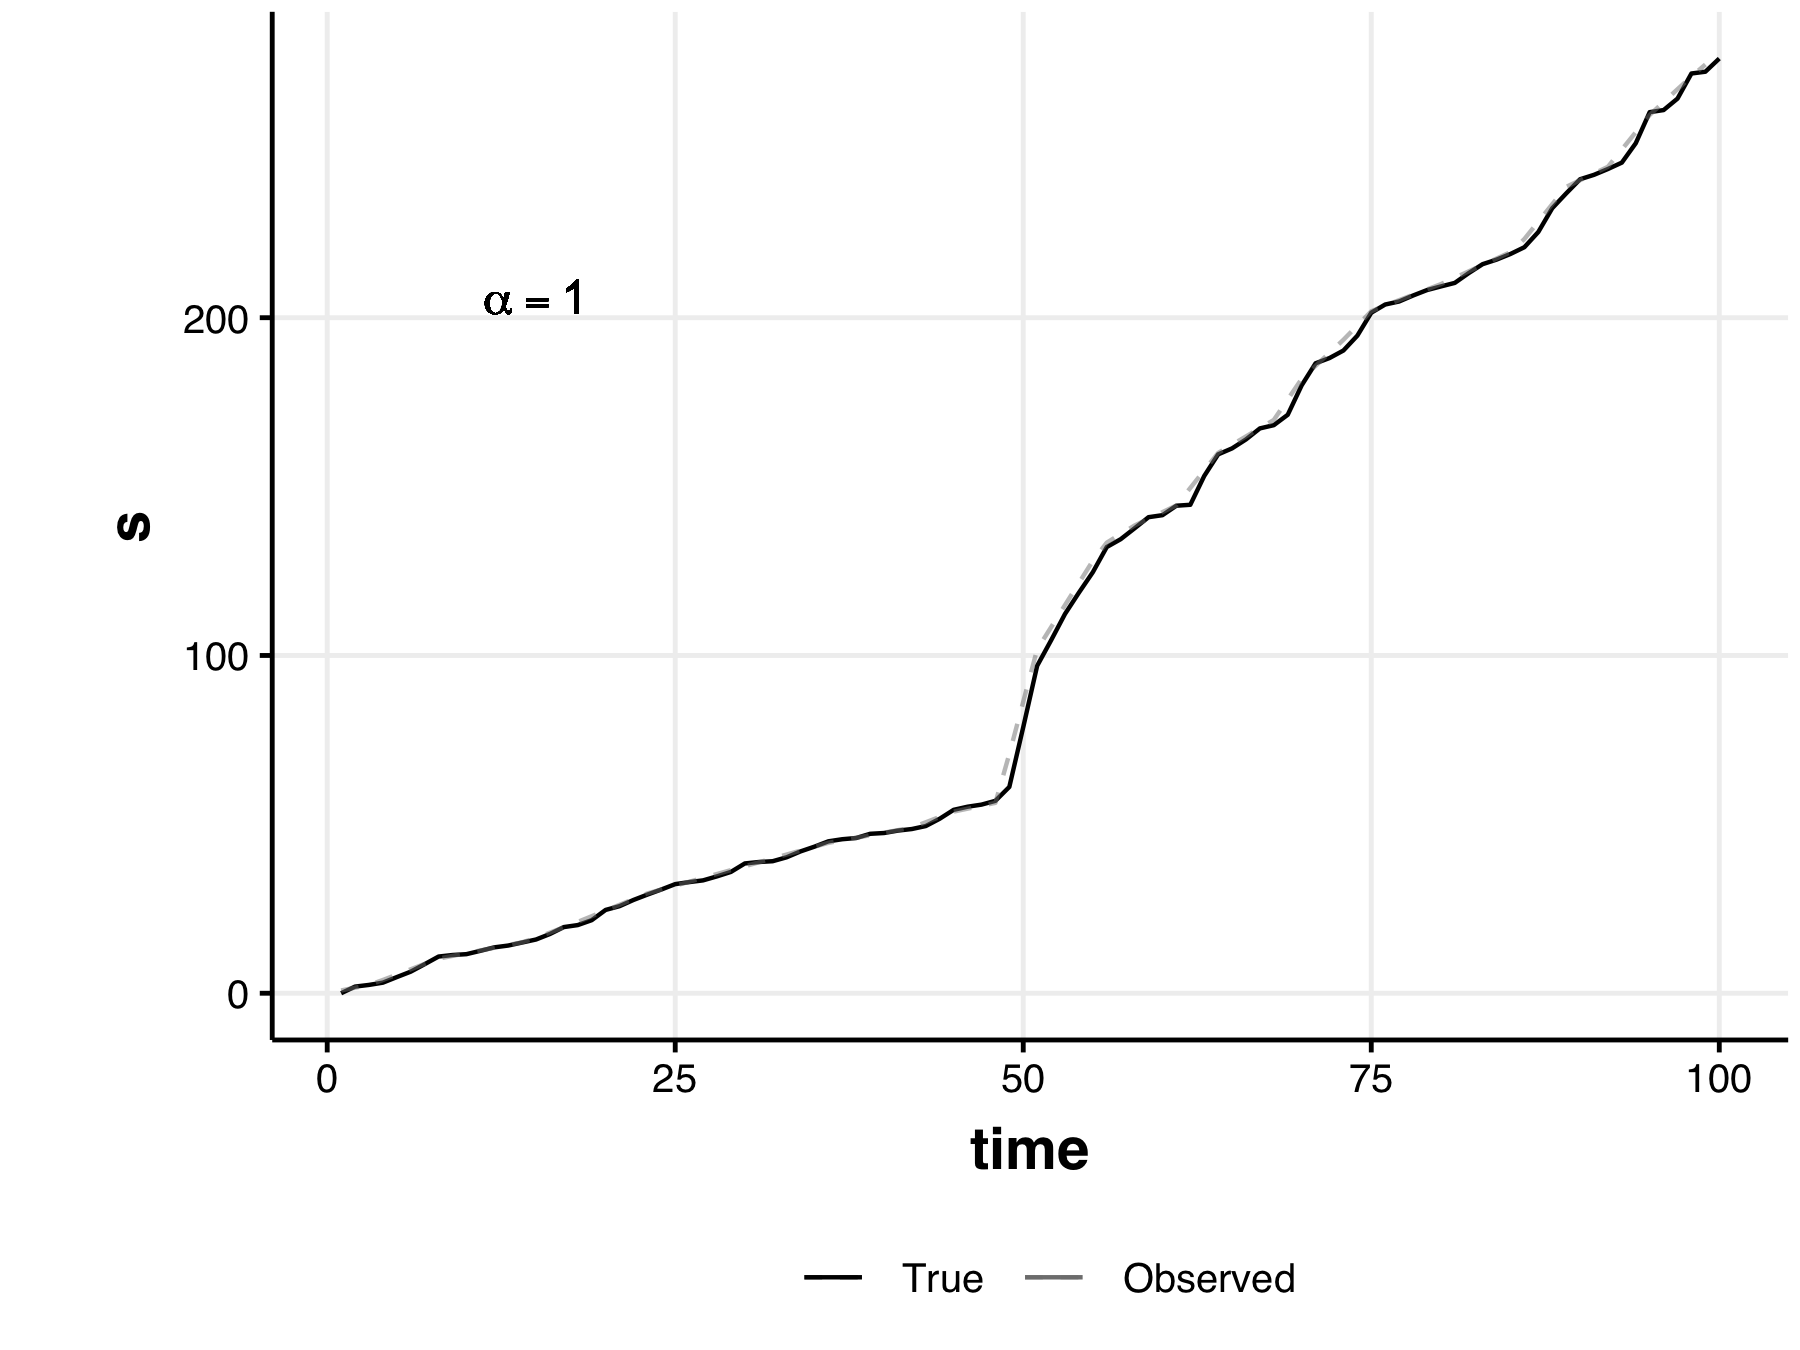
\includegraphics[width=0.33\linewidth]{/Users/jessicaburnett/Documents/GitHub/myDissertation//chapterFiles/velocity/figsCalledInDiss/compareTvdiff_s_changeMuX1_tanhAlpha1-1tvdiffAlpha-1000iter} \caption{Comparison of the antidifferentiated values ('observed') of the distance travelled, $s$, to the true process values of $s$ ('true) provides a method for identifying the best values of the smooothing parameter, $\alpha$. Under most conditions $\alpha \ll$ sufficed. Here, we compare the true and antidifferentiated values of $s$ under the condition of changing $\mu_{x1}$ when the hyperbolic tangent function is most rapid ($\alpha_{tanh}=1$) for the `tvdiff` alpha values of: $\alpha=0.50$ (top), $\alpha=1$ (middle), and $\alpha=10$ (bottom). Notice that the antidifferentiated $s$ (observed) is increasingly smoothed as $\alpha$ increases.}\label{fig:antiDiffComp}
\end{figure}
\begin{figure}
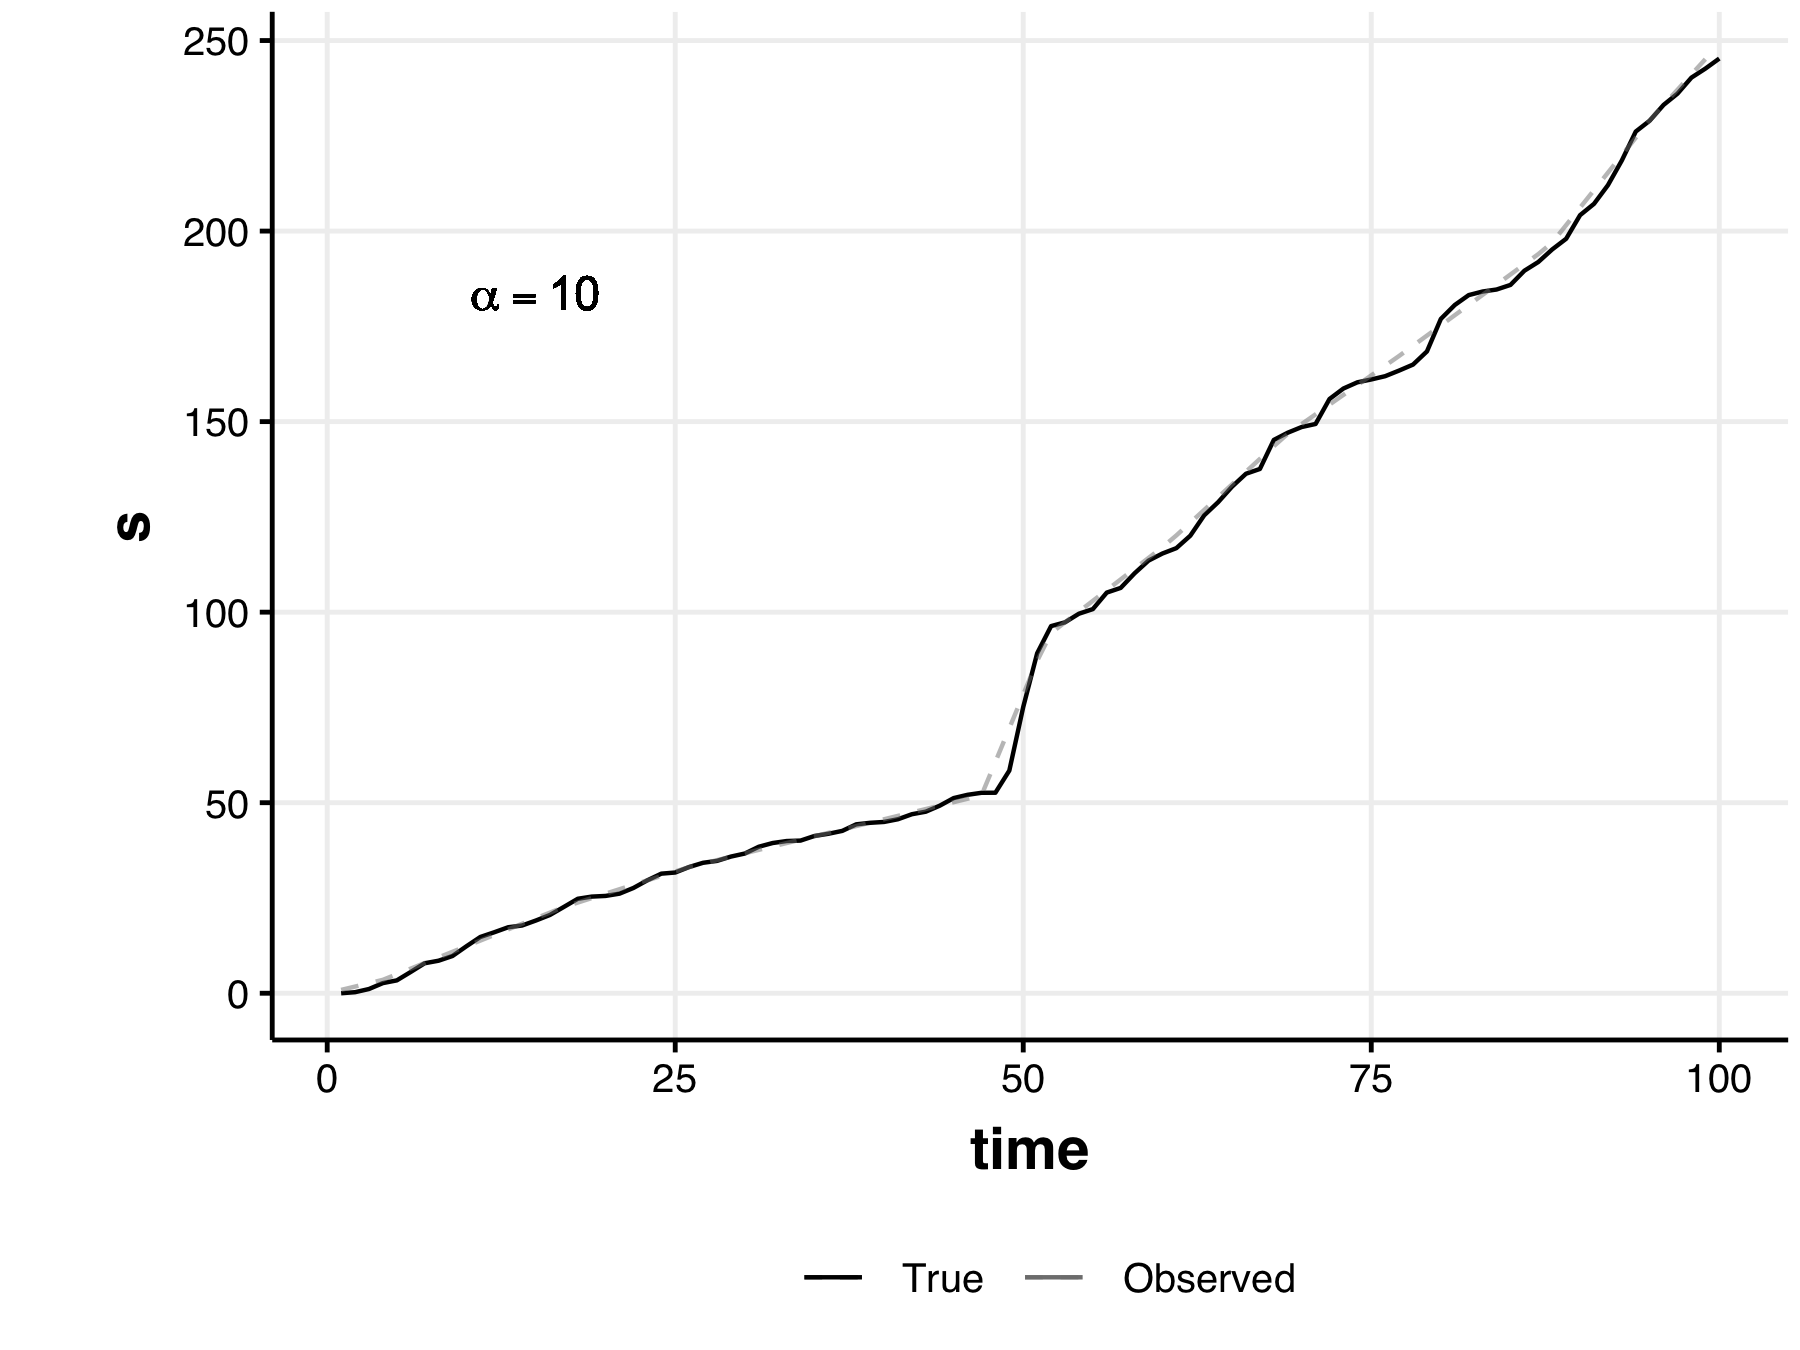
\includegraphics[width=0.33\linewidth]{/Users/jessicaburnett/Documents/GitHub/myDissertation//chapterFiles/velocity/figsCalledInDiss/compareTvdiff_s_changeMuX1_tanhAlpha1-10tvdiffAlpha-1000iter} \caption{Comparison of the antidifferentiated values ('observed') of the distance travelled, $s$, to the true process values of $s$ ('true) provides a method for identifying the best values of the smooothing parameter, $\alpha$. Under most conditions $\alpha \ll$ sufficed. Here, we compare the true and antidifferentiated values of $s$ under the condition of changing $\mu_{x1}$ when the hyperbolic tangent function is most rapid ($\alpha_{tanh}=1$) for the `tvdiff` alpha values of: $\alpha=0.50$ (top), $\alpha=1$ (middle), and $\alpha=10$ (bottom). Notice that the antidifferentiated $s$ (observed) is increasingly smoothed as $\alpha$ increases.}\label{fig:antiDiffComp}
\end{figure}
\hypertarget{smooth-changes-in-the-mean}{%
\subsubsection{Smooth changes in the mean}\label{smooth-changes-in-the-mean}}

As discussed earlier, the velocity of the distance travelled, \(v\), is a measure of how quickly the sum of the squared system variables change between observations (i.e.~time). Consequently, as the total change in state variables grows, so will the maximum potential of the velocity, \(v\). Following this logic, we should expect to see a spike in the derivative of the distance travelled when the system changes quickly. I tested this hypothesis under two conditions of changing means, where either one or both variables underwent mean shifts (see Table \ref{tab:params}), and under varying degrees of transition smooothness (i.e.~\(\alpha_{tanh}={0.25, 0.50, 0.75, 1.00}\)).

When the hyperbolic tangent smooth transition function is less steep (@ref(fig:mu1var.25)) the observed velocity signal is dampened. This signal, however, is quickly recovered when the transition function becomes more abrupt (Figs. @ref(fig:mu1var.5),@ref(fig:mu1var.75,\ref{fig:mu1var1}; \(\alpha_{tanh}=0.5, 0.75, and 1.00\), respectively). Unsurprisingly, when we shift the means of both state variables while holding the relative variance constant, the velocity signal changes more abruptly (Fig. @ref(fig:muBoth.25)) than when only a single variable shifts mean value (compare with Fig. @ref(mu1Var.25)). Figure @ref(muBoth.75) is representative of the increasing signal in velocity as \(\alpha_{tanh}\) increases.
\begin{figure}
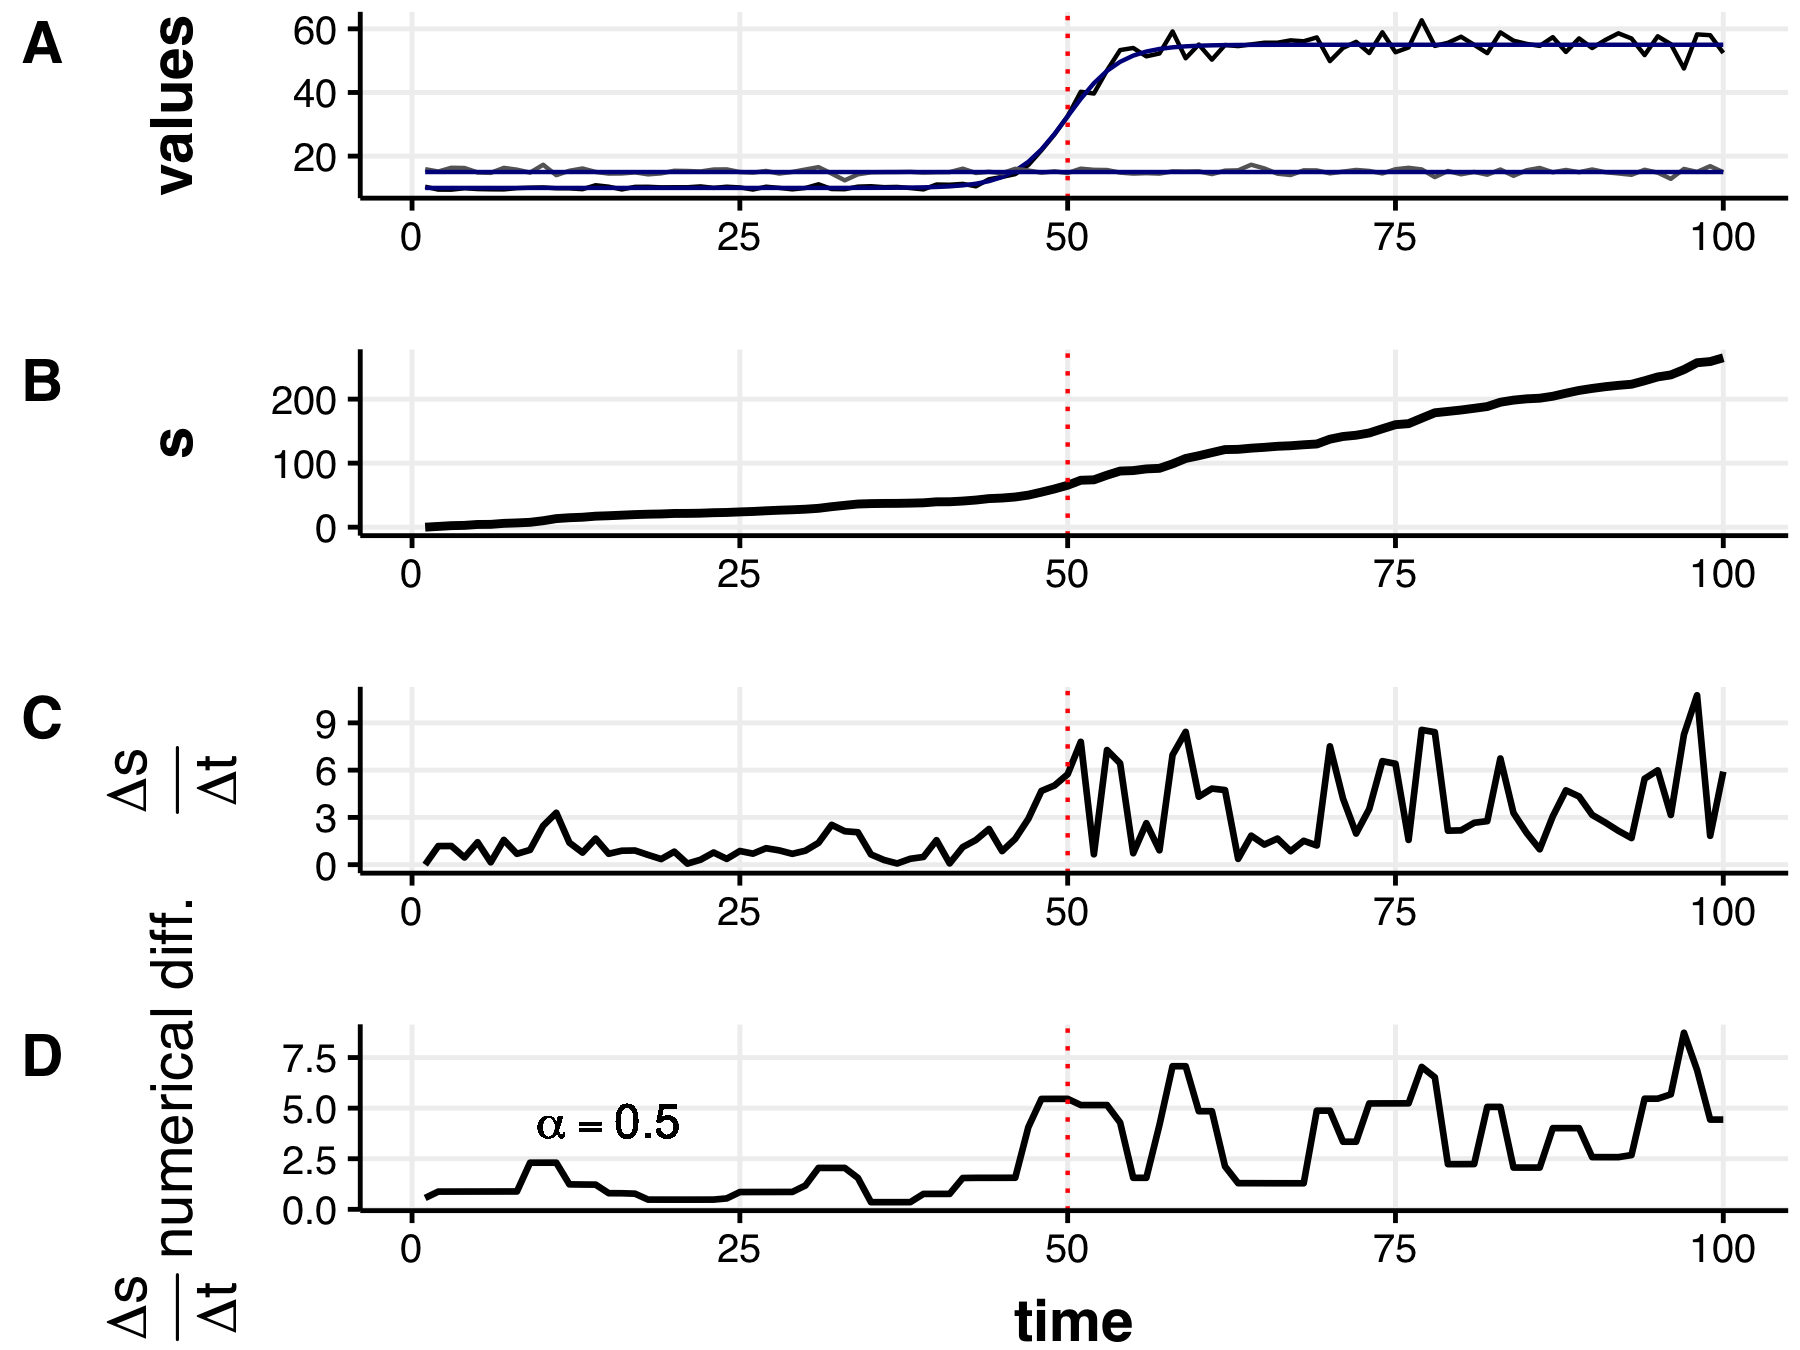
\includegraphics[width=0.85\linewidth]{/Users/jessicaburnett/Documents/GitHub/myDissertation/chapterFiles/velocity/figsCalledInDiss/changeMuX1_tanhAlpha025-05tvdiffAlpha-1000iter_stackTvdiff} \caption{The velocity signal is muted when the  hyperbolic smoothing parameter, $\alpha$, is low (0.25). True and observed values of $x_i$ (panel A), observed distance travelled ($s$, panel B), observed velocity (C), and the smoothed velocity (D). }(\#fig:mu1var.25)
\end{figure}
\begin{figure}
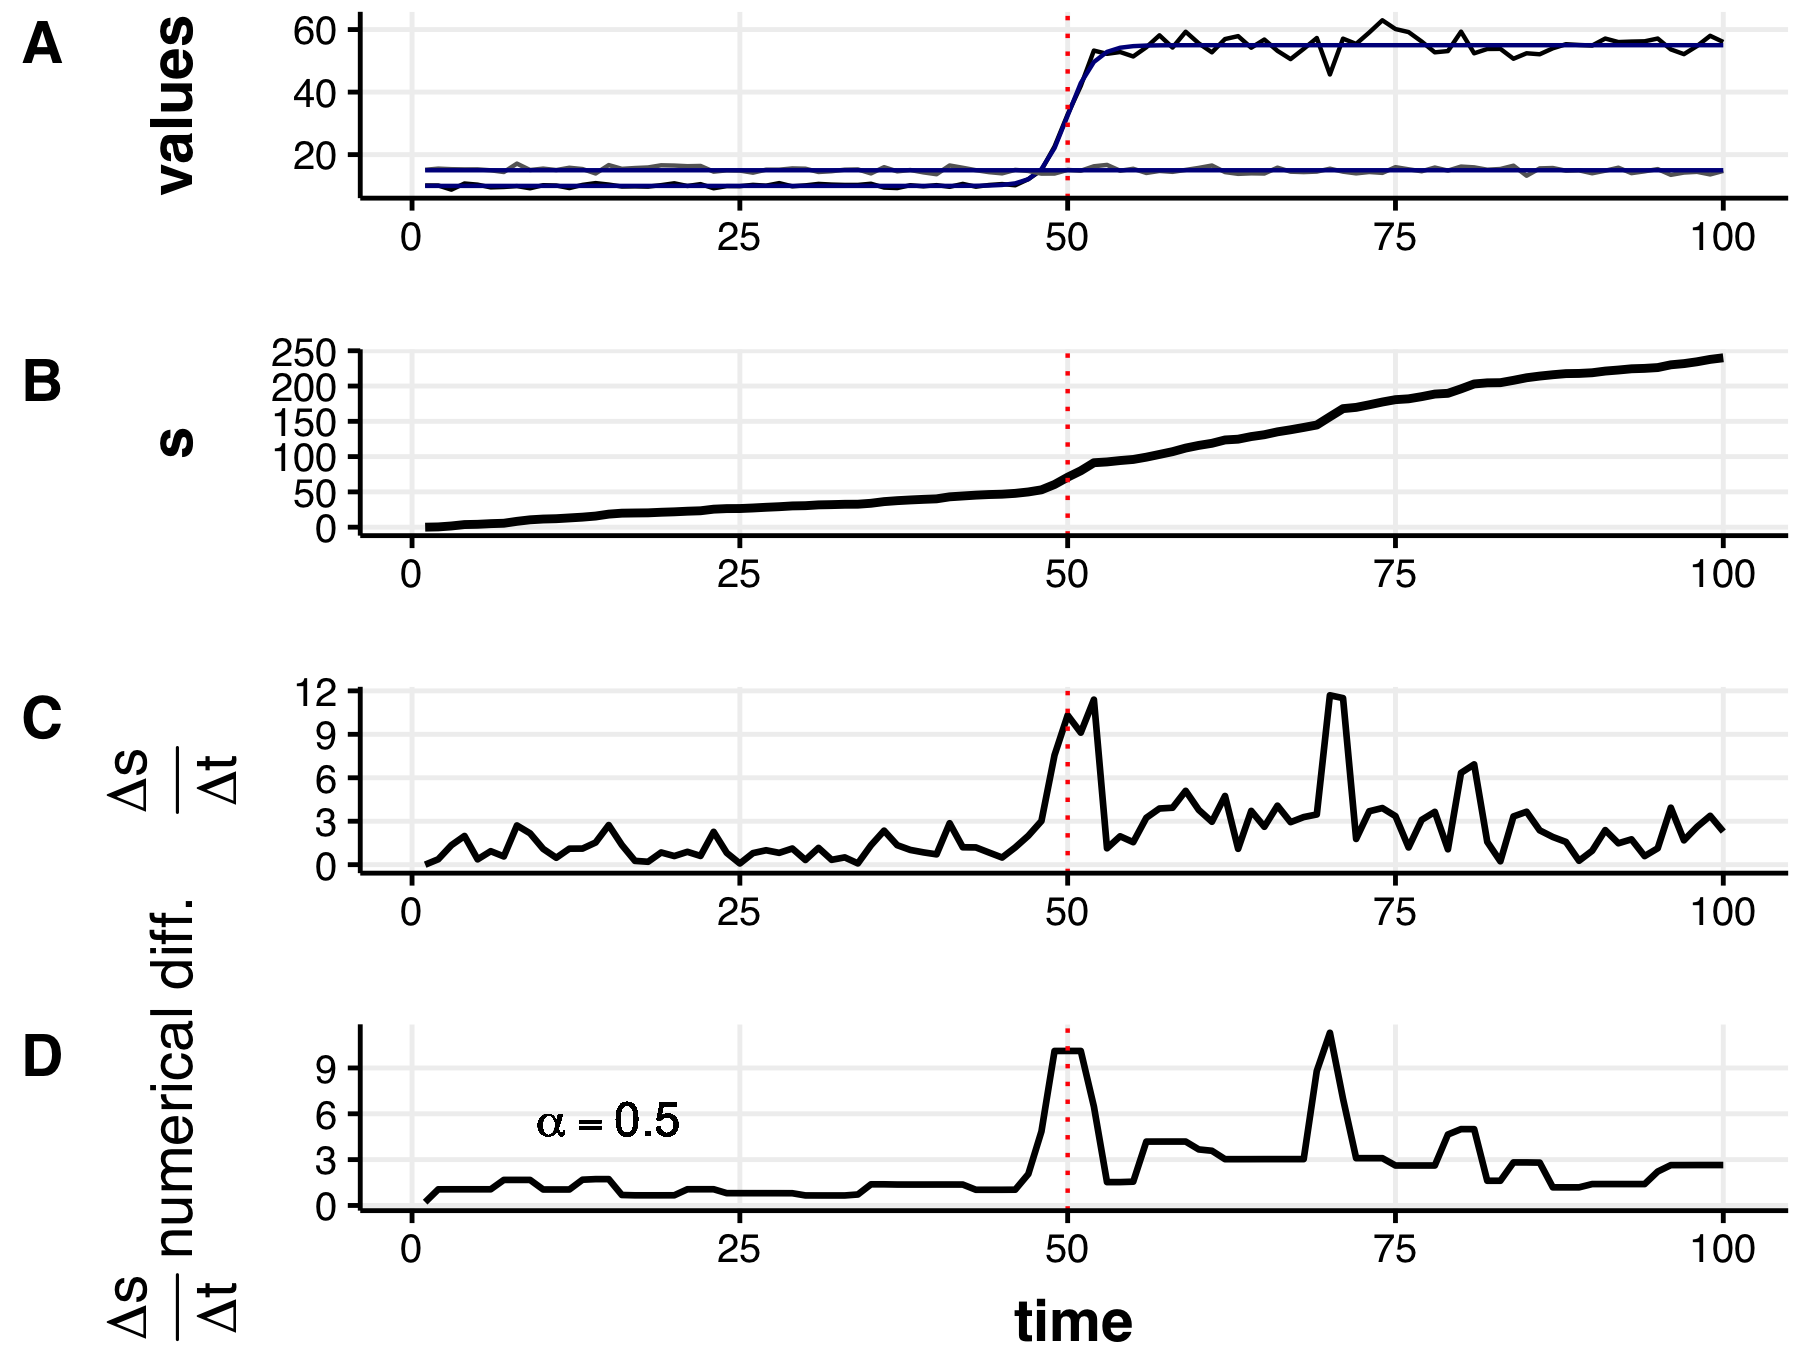
\includegraphics[width=0.85\linewidth]{/Users/jessicaburnett/Documents/GitHub/myDissertation/chapterFiles/velocity/figsCalledInDiss/changeMuX1_tanhAlpha05-05tvdiffAlpha-1000iter_stackTvdiff} \caption{The velocity signal is muted when the  hyperbolic smoothing parameter, $\alpha$, is moderate (0.50). True and observed values of $x_i$ (panel A), observed distance travelled ($s$, panel B), observed velocity (C), and the smoothed velocity (D). }(\#fig:mu1var.5)
\end{figure}
\begin{figure}
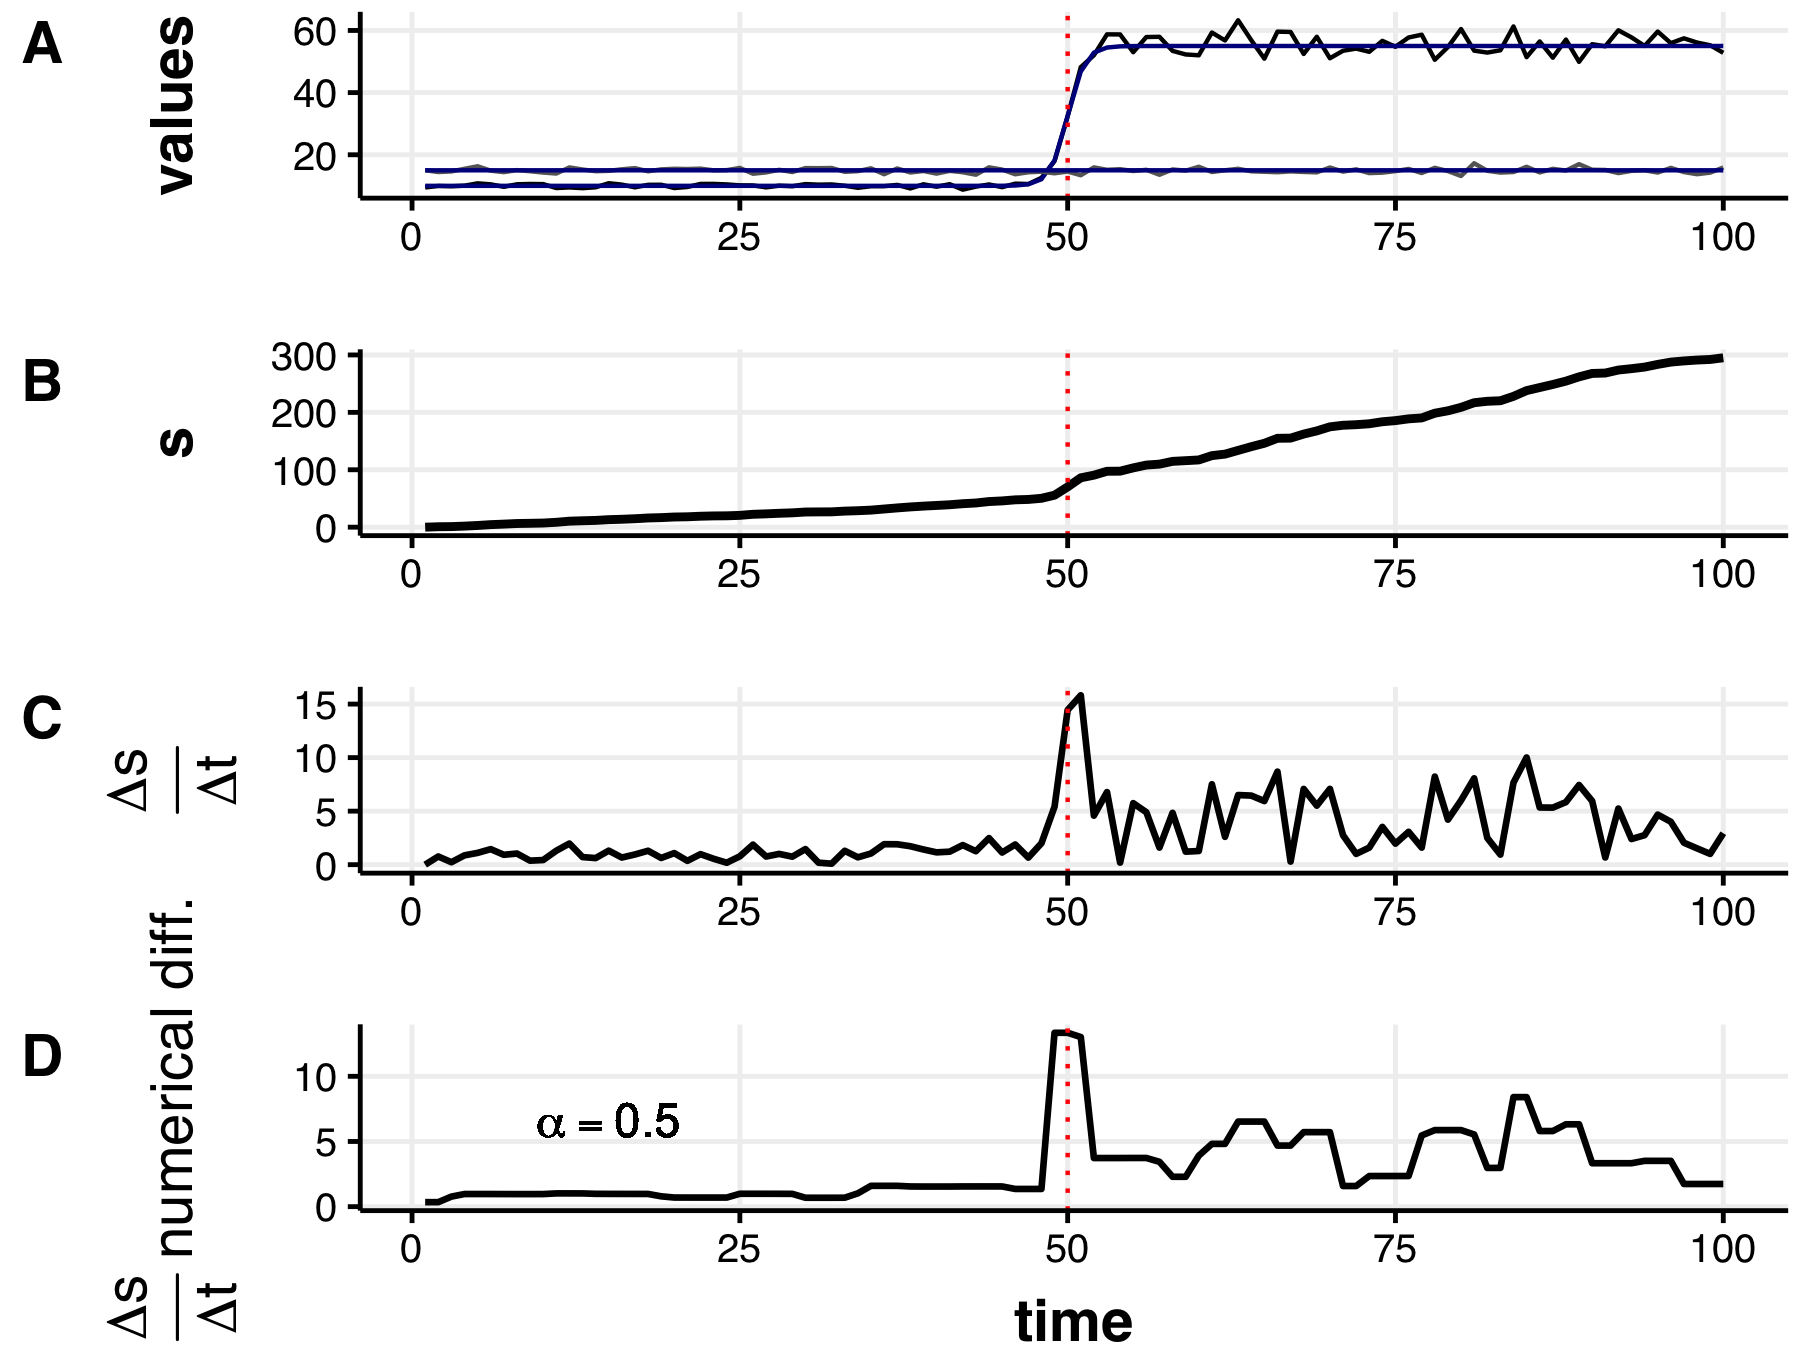
\includegraphics[width=0.85\linewidth]{/Users/jessicaburnett/Documents/GitHub/myDissertation/chapterFiles/velocity/figsCalledInDiss/changeMuX1_tanhAlpha075-05tvdiffAlpha-1000iter_stackTvdiff} \caption{The velocity signal is muted when the  hyperbolic smoothing parameter, $\alpha$, is moderate (0.50). True and observed values of $x_i$ (panel A), observed distance travelled ($s$, panel B), observed velocity (C), and the smoothed velocity (D). }(\#fig:mu1var.75)
\end{figure}
\begin{figure}
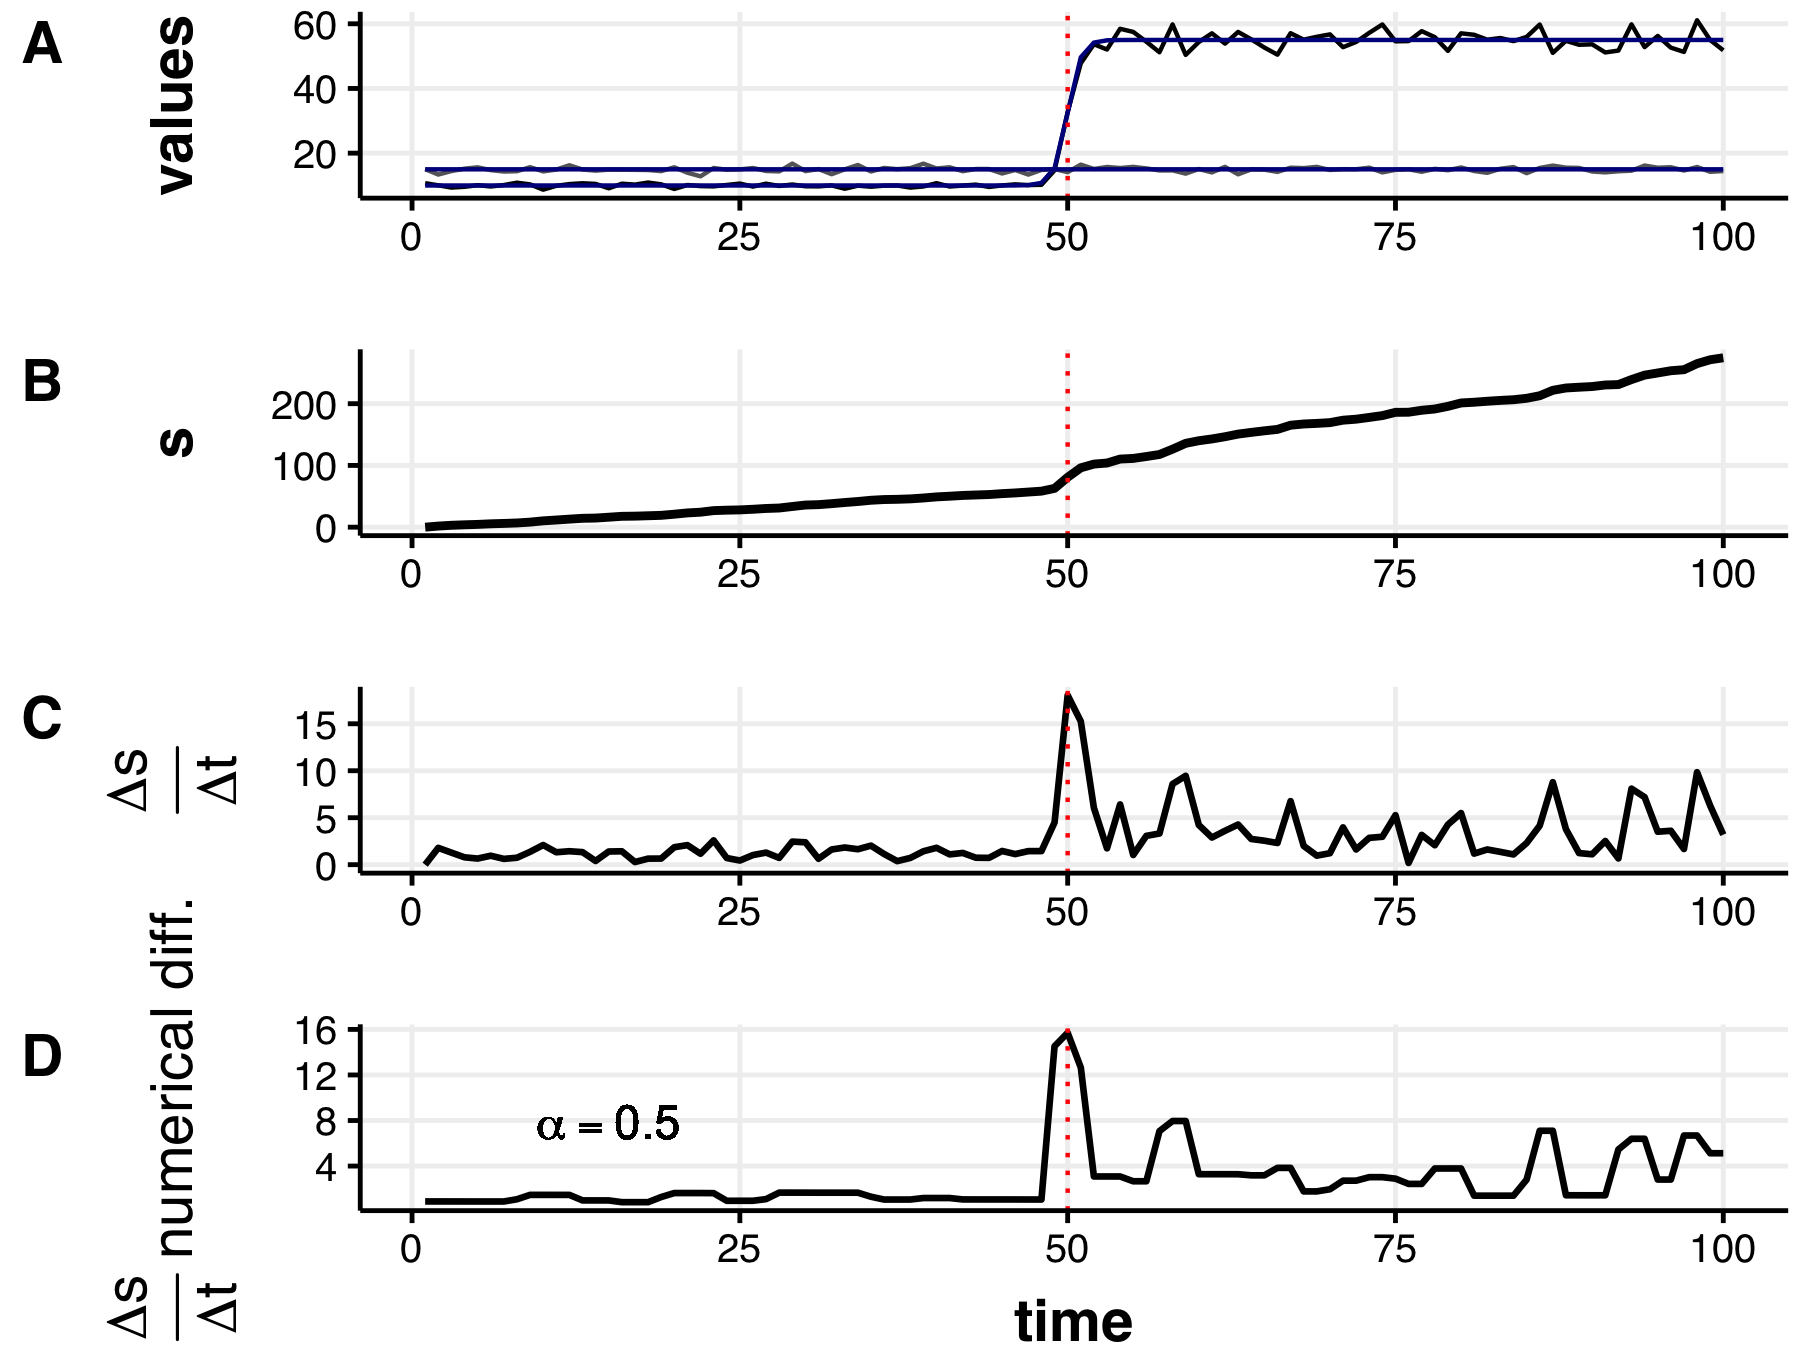
\includegraphics[width=0.85\linewidth]{/Users/jessicaburnett/Documents/GitHub/myDissertation/chapterFiles/velocity/figsCalledInDiss/changeMuX1_tanhAlpha1-05tvdiffAlpha-1000iter_stackTvdiff} \caption{The velocity signal is muted when the  hyperbolic smoothing parameter, $\alpha$, is moderate (0.50). True and observed values of $x_i$ (panel A), observed distance travelled ($s$, panel B), observed velocity (C), and the smoothed velocity (D). }\label{fig:mu1var1}
\end{figure}
\begin{figure}
\includegraphics[width=0.85\linewidth]{/Users/jessicaburnett/Documents/GitHub/myDissertation/chapterFiles/velocity/figsCalledInDiss/changeMuBoth_tanhAlpha025-05tvdiffAlpha-1000iter_stackTvdiff} \caption{The velocity signal is regained under smoooth transition ($\alpha_{tanh}=0.25$) when both state variables undergo a shift in the mean. True and observed values of $x_i$ (panel A), observed distance travelled ($s$, panel B), observed velocity (C), and the smoothed velocity (D). }(\#fig:muBoth.25)
\end{figure}
\begin{figure}
\includegraphics[width=0.85\linewidth]{/Users/jessicaburnett/Documents/GitHub/myDissertation/chapterFiles/velocity/figsCalledInDiss/changeMuBoth_tanhAlpha075-05tvdiffAlpha-1000iter_stackTvdiff} \caption{The velocity signal is regained under smoooth transition ($\alpha_{tanh}=0.75$) when both state variables undergo a shift in the mean. True and observed values of $x_i$ (panel A), observed distance travelled ($s$, panel B), observed velocity (C), and the smoothed velocity (D). }(\#fig:muBoth.75)
\end{figure}
\hypertarget{smooth-changes-in-variance}{%
\subsubsection{Smooth changes in variance}\label{smooth-changes-in-variance}}

Abrupt changes sometimes manifest first as a change in the variability, rather than the mean value, of the state variables. This condition manifests in the velocity signal when both variables experience a shift in relative variance (Fig. \ref{fig:varBoth}), however, does not signal change when only one variable exhibits a shift in variance (Fig. \ref{fig:var1}). Again, given the total magnitude of change influences the distance travelled, \(s\), and the derivative of s, \(v\), it is not surprising that the velocity signal is greater around the transition point when both, compared to a single, state variable exhibits increased variability about the mean. In these scenarios I shifted the variability in the state variables \(x_i\) from only \(\sim 5\%\) to \(\sim10\%\) (see Table \ref{tab:params})---this percent variability is low relative to most empirical observational ecological datasets. As such, I expect the velocity signal to be more pronounced when empirical systems undergo shifts in variance in at least one state variable.
\begin{figure}
\includegraphics[width=0.85\linewidth]{/Users/jessicaburnett/Documents/GitHub/myDissertation/chapterFiles/velocity/figsCalledInDiss/changeVarBoth_tanhAlpha075-5tvdiffAlpha-1000iter_stackTvdiff} \caption{The velocity signals a rapid shift in the variance of both state variables under a moderately abrupt transition ($\alpha_{tanh}=0.75$). True and observed values of $x_i$ (panel A), observed distance travelled ($s$, panel B), observed velocity (C), and the smoothed velocity (D). }\label{fig:varBoth}
\end{figure}
\begin{figure}
\includegraphics[width=0.85\linewidth]{/Users/jessicaburnett/Documents/GitHub/myDissertation/chapterFiles/velocity/figsCalledInDiss/changeVarX1_tanhAlpha075-10tvdiffAlpha-1000iter_stackTvdiff} \caption{The velocity does not signal shifts in the variance of a single variable ($x_1$) under a moderately abrupt transition ($\alpha_{tanh}=0.75$). True and observed values of $x_i$ (panel A), observed distance travelled ($s$, panel B), observed velocity (C), and the smoothed velocity (D). }\label{fig:var1}
\end{figure}
\hypertarget{smooth-changes-in-the-mean-and-variance}{%
\subsubsection{Smooth changes in the mean and variance}\label{smooth-changes-in-the-mean-and-variance}}

Given the signals identified in the velocity when one or both state varialbes exhibits a shift in mean and/or variance, it is unsurprising that even under smooth transitions (when \(\alpha_{tanh} = 0.25\)), velocity manifests as a signal of change (Fig. @ref(muVarBoth.25)). This signal is most pronounced when the shift is abrupt (Fig. \ref{muVarBoth1})
\begin{figure}
\includegraphics[width=0.85\linewidth]{/Users/jessicaburnett/Documents/GitHub/myDissertation/chapterFiles/velocity/figsCalledInDiss/changeMuVarBoth_tanhAlpha025-5tvdiffAlpha-1000iter_stackTvdiff} \caption{The velocity signals a shift when both variables undergo shifts in the mean and variance under a slightly abrupt transition ($\alpha_{tanh}=0.25$). True and observed values of $x_i$ (panel A), observed distance travelled ($s$, panel B), observed velocity (C), and the smoothed velocity (D). }(\#fig:muVarBoth.25)
\end{figure}
\begin{figure}
\includegraphics[width=0.85\linewidth]{/Users/jessicaburnett/Documents/GitHub/myDissertation/chapterFiles/velocity/figsCalledInDiss/changeMuVarBoth_tanhAlpha1-10tvdiffAlpha-1000iter_stackTvdiff} \caption{The velocity signals a shift when both variables undergo shifts in the mean and variance under a slightly abrupt transition ($\alpha_{tanh}=1.00$). True and observed values of $x_i$ (panel A), observed distance travelled ($s$, panel B), observed velocity (C), and the smoothed velocity (D). }\label{fig:muVarBoth1}
\end{figure}
\hypertarget{velocity-performance-under-empirical-transitions-paleolithic-freshwater-diatom-community}{%
\section{Velocity performance under empirical transitions: paleolithic freshwater diatom community}\label{velocity-performance-under-empirical-transitions-paleolithic-freshwater-diatom-community}}
\begin{figure}
\includegraphics[width=0.85\linewidth]{/Users/jessicaburnett/Documents/GitHub/myDissertation/chapterFiles/velocity/figsCalledInDiss/paleoTurnover} \caption{Relative abundances of the most common diatom species in the time series. Few species dominate the data over the entire time series, and turnover is apparent at multiple observations.}\label{fig:paleoTurnover}
\end{figure}
To gather baseline information on the use of velocity in empirical systems data, I calculated velocity for the paleodiatom system described in Chapter \ref{resampling} (see also Appendix \ref{appPaleo}. Briefly, the paleodiatom community comprises 109 time series over a period of approximately 6936 years (Fig. \ref{fig:paleoTurnover}). As elaborated in Spanbauer et al. (2014), the paleodiatom community is suggested to have undergone regime shifts at multiple points. These abrupt changes are apparent when exploring the relative abundaces over time, as there are extreme levels of species turnover at multiple points in the data (Fig. \ref{fig:paleoTurnover}). Using Fisher Information and climatological records, Spanbauer et al. (2014) suggest that regime shifts in this system at approximately 1,300 years before present (where present is equal to year 1950).
\begin{figure}
\includegraphics[width=0.85\linewidth]{/Users/jessicaburnett/Documents/GitHub/myDissertation/chapterFiles/velocity/figsCalledInDiss/paleoVelocity} \caption{Velocity $v$ and distance travelled $s$ of the paleodiatom time series. Dashed line at 1,300 years before 1950 indicates the regime shift identifed in Spanbauer et al. (2014). Dotted lines indicate regime shifts as visually identified on metrics $s$ and $v$.}\label{fig:paleoVelocity}
\end{figure}
\begin{figure}
\includegraphics[width=0.85\linewidth]{/Users/jessicaburnett/Documents/GitHub/myDissertation/chapterFiles/velocity/figsCalledInDiss/paleoRegime1and3} \caption{Velocity ($v$) indicates periodic-like conditions in the first (A) and second (B) regimes.}\label{fig:paleoRegime1and3}
\end{figure}
Spanbauer et al. (2014) used different regime detection metrics coupled with regional climatological events to identify regime shifts in the system, suggest that a regime shift occurred at \textasciitilde1,300 years before present. Using the methods outlined above, I calculated the distance travelled (\(s\)) and velocity (\(v\); Fig. \ref{fig:paleoV}). The results of \(v\) and \(s\) (\ref{fig:paleoVelocity}) on the relative abundance data correspond with both the large shifts in species dynamics (see Fig \ref{fig:paleoTurnover}, and also with the regime shift identified by Spanbauer et al. (2014). However, two primary results can be made from the metrics \(v\) and \(s\) that are not obvious nor identified numerically in the results of Spanbauer et al. (2014) ():
1. Two additional large shifts occurred at approximately 2,500, 4,800 and years before 1950\\
1. The periods before the first and after the second large shifts appear oscillatory (Fig. \ref{fig:paleoRegime1and3}).\\
To determine whether removing the noise in the data, I interpolated the each time series using function \texttt{stats::approx} to 700 time points. Next, I calculated the distance travelled of the entire system, \(s\). Finally, I obtained the derivative of \(s\) by using a regularized differentiation (using function \texttt{tvdiff::TVRegDiffR}; parameters were \(iter = 2000\), scale = small, \(ep = 1 x 10^-6\), and \(\alpha = 100\)). This method of regularized differentiation is an ideal approach to smoothing \(s\) because it assumes the data are non-smooth and incorporates finite differencing. The total variation regularized differentiation is desribed in Chartrand (2011), Price \& Burnett (2019), and in the previous first-level section.
\begin{figure}
\includegraphics[width=0.85\linewidth]{/Users/jessicaburnett/Documents/GitHub/myDissertation/chapterFiles/velocity/figsCalledInDiss/paleoObsPred} \caption{The regularized differentiation of $s$ was best fit using $\alpha = 100$. Higher overlap of $s$ and pred indicates a good fit of the regularized differentiated metric to the non-smoothed metric, $s$.}\label{fig:paleoObsPred}
\end{figure}
The smoothed velocity (\ref{fig:paleoV}) provides a similar but smoother picture of the velocity of the system trajectory. Comparing the smoothed (\ref{fig:paleoV}) to the non-smoothed velocity (\ref{fig:paleoVelocity}) yields similar inference regarding the location of the regime shifts at 2,200 and 1,300 years before present, however, it more clearly demonstrates potential inter-regime dynamics (e.g., between 7,000 and 4,800 years before present), which were not identified in previous study of this ssytem (Spanbauer et al., 2014).
\begin{figure}
\includegraphics[width=0.85\linewidth]{/Users/jessicaburnett/Documents/GitHub/myDissertation/chapterFiles/velocity/figsCalledInDiss/paleoV} \caption{The velocity metric  ($v$) signals potential periodicities in the paleo diatom time series data when the distance travelled metric, $s$, is smoothed using regularized differentiation methods [@price2019tvdiff].}\label{fig:paleoV}
\end{figure}
\hypertarget{discussion-3}{%
\section{Discussion}\label{discussion-3}}

Here, I described the steps for calculating a novel regime detection metric, system velocity (\(v\)). First described in Fath et al. (2003), \(v\) is used as a single step for caclulating a more complicated regime detection metric, Fisher Information (see also Chapter \ref{fiGuide}). System velocity is arguably simple to calculate, as shown in this chapter, captures the total change in system variables under a variety of mean and variance conditions. The metric does not, however, perform well as variance increases (Fig. \ref{simVarPlot2}), and smooothing the original data does not reduce the noise surrounding this metric when variance is moderate (Fig. \ref{smoothV}). Variance is a commonly-used indicator of ecological regime shifts (Brock \& Carpenter (2006)), however, is difficult to interpret when the number of variables is \(\ggg\) a few. System velocity, \(v\), may be useful in situations where the number of state variables is \(\ggg\) few, and appears especially useful when the magnitude of change in one or more state variables is high (Figs. \ref{fig:simVplot2},@ref(fig:muBoth.75)). For example, this method will likely identify signals of regime shifts where the shift is defined as high species turnover within a community (Fig. \ref{fig:muVarBoth1}).

This study provides baseline expectations of the velocity of the distance travelled, \(V\), as an indicator of abrupt change in a multivariable system. Although a useful first step, this metric should next be critiqued in a sensitivity analytical approach, where a statistical measure is used to determine whether \(V\) indicates abrupt shifts prior to occurrence (c.f. during or after), particularly with respect to its performance in community-level empirical data. The paleolitic diatom data used in the last section of this chapter is also presented in the documentation for my R Package, \textbf{regimeDetectionMeasures} (Appendix \ref{appPaleo}). In this case study, the `distance travelled', \(s\) (Eq. \eqref{eq:diffXsq2}), clearly exhibits shifts at points where expert opinion and species turnover (in species dominance) agree that a large change occurred. Further, velocity, \(v\) (see \emph{dsdt} in package materials) indicates a large shift at only the most predonimnant shift in the time series, perhaps due to the metric's sensitivity to variance (Fig. \ref{fig:simVplot2}.

Further work is required to determine the utility of system velocity as a regime detection metric, however, this chapter demonstrates that the metric may indicate clear shifts in variable means and variability about the means. In addition to examining high-dimensional and noisy data, a study of the performance of \(v\) under conditions where few variables exhibit large changes while many variables are relatively constant may also prove useful. Additionally, this metric may be a useful tool for reducing the dimensionality of high dimensional data. Although the metric loses much information, as opposed to some dimension reduction techniques, e.g.~Principal Components Analysis PCA, the metric is simple to calculate (even by hand), is computationally inexpensive, and is intuitive, unlike many clustering algorithms (e.g., Non-metric Multidimensional Scaling NMDS). Like system velocity, methods of the latter variety (e.g.~NMDS) require post-hoc statistical analyses to confirm the location of clusters (or abrupt change, regime shifts), while methods of the former variety (e.g.~PCA) retain loadings but do not necessarily identify the locations of abrupt shifts.

\hypertarget{supplementary-figures}{%
\section{Supplementary Figures}\label{supplementary-figures}}

This section contains additional examples of the behavior of velocity, \(v\) when varying the mean and/or variance prior to and/or after the induced abrupt shiftt in the toy system with a discontinuous transition at \(t=50\).
\begin{figure}
\includegraphics[width=0.85\linewidth]{_myDissertation_files/figure-latex/velocSysEx2-1} \caption{System change ($s$) and velocity ($v$) of the model system over the time period. Change in means ($\bar{x}_{1_{pre}}=25$, $\bar{x}_{1_{post}}=100$, $\bar{x}_{2_{pre}}=50$, $\bar{x}_{2_{post}}=10$) and an increase in variance ($\sigma_{1_{pre}}=2$, $\sigma_{1_{post}}=10$, $\sigma_{2_{pre}}=5$,  $\sigma_{2_{post}}=10$).}\label{fig:velocSysEx2}
\end{figure}
\begin{figure}
\includegraphics[width=0.85\linewidth]{_myDissertation_files/figure-latex/velocSysEx3-1} \caption{System change ($s$) and velocity ($v$) of the model system over the time period. Constant means ($\bar{x}_1=25$, $\bar{x}_2=50$) and sharp change in variance for one state variable $\sigma_{1_{pre}} = 2$, $\sigma_{1_{post}} = 12$, $\sigma_{2_{pre,post}} = 5$}\label{fig:velocSysEx3}
\end{figure}
\begin{figure}
\includegraphics[width=0.85\linewidth]{_myDissertation_files/figure-latex/velocSysEx4-1} \caption{System change ($s$) and velocity ($v$) of the model system over the time period. Variance equal to mean ($/bar{x_i}=/sigma_i$), where means ($/bar{x}_{1_{pre}}=25$, $/bar{x}_{1_{post}}=50$, $/bar{x}_{2_{pre}}=15$, $/bar{x}_{2_{post}}=150$).}\label{fig:velocSysEx4}
\end{figure}
\hypertarget{resampling}{%
\chapter{Robustness of Multivariate Regime Detection Measures to Varying Data Quality and Quantity Using Resampling}\label{resampling}}

\hypertarget{introduction-4}{%
\section{Introduction}\label{introduction-4}}

Ecological systems have many unpredictable and variably interacting components (J??rgensen et al., 2011). Methods for analyzing these complex systems, e.g.~Dynamic Bayesian Networks, network models, and food webs are designed to handle these complexities, yet require data- and knowledge-intensive models. Although ecological data collection and data management techniques are improving (La Sorte et al., 2018), the aforementioned approaches to modeling and understanding complex system are often infeasible in ecosystem research and management (Clements \& Ozgul, 2016).

A growing concern with anthropogenic impacts on the environment has increased the demand for mathematical and statistical techniques that capture these dynamics. These often undesirable changes in the structure or functioning of ecological systems are often referred to as \emph{regime shifts}, \emph{regime changes}, \emph{state change}, \emph{abrupt change}, etc. (Andersen et al., 2009) . A yet-unattained goal of ecological research and management is to reach a point where these methods can predict impending regime shifts in real-time and with high confidence. Ideally, ecological regime shift detection methods (hereafter, regime detection measures) would require little knowledge of the intrinsic drivers of the system, and the users of the method would not be required to know if and where a regime shift occurred in the data.

Despite the suite of regime detection measures in the environmental and ecological research literatures, they are not used in ecological management. We can describe the current state of regime detection measures as being either system specific (i.e., the method is not system agnostic) or not. Methods of the latter type are convenient in that they can be applied across various system and data types, but the results of these analyses require some degree of subjective interpretation (Clements \& Ozgul, 2018; \emph{c.f.} Batt, Carpenter, Cole, Pace, \& Johnson, 2013). Efforts to develop and/or improve regime detection measures that do not require such subjectivity will aid the advance of regime detection measures research and application.

Current efforts to improve regime detection measures may be stunted by the lack of application beyond simple and/or theoretical (toy) systems data. Like most statistical and mathematical approaches, the evolution of many regime detection measures begins with application to theoretical data, followed by application to empirical data. Current applications of regime detection measures to empirical, ecological data are largely limited to data describing populations (Alheit et al., 2005; Anderson \& Piatt, 1999; deYoung et al., 2008), climatic, marine, and Paleolithic regime shifts (Kong et al., 2017; Spanbauer et al., 2014; Yang \& Wu, 2006), with few applications to terrestrial data (\emph{c.f.} Bahlai, Werf, O'Neal, Hemerik, \& Landis, 2015; Sundstrom et al., 2017). Although testing the performance and inference boundaries of theoretical and simple systems is important, they are of little use to ecosystem managers if they are not proven to be easily and reliably applicable to their system. Additionally, regime detection measures should be capable of handling empirical ecological data, which are often sparse, noisy, and irreguarly sampled..

Ecological systems data is expensive to capture, and has large process variation and observation errors. This variability reduces data quality and quantity, limiting the numerical tools for identifing trends and changes in the system (Thrush et al., 2009). Some methods, new and old, proposed as regime detection measures are purported to handle the data limitation and quality issues inherent in ecological data, and minimize subjective decisions for choosing state variables and interpreting results. For example, variable reduction techniques, e.g.~principal components analysis (Andersen et al., 2009; Reid et al., 2016; S. Rodionov \& Overland, 2005), clustering algorithms (Weijerman, Lindeboom, \& Zuur, 2005; Weissmann \& Shnerb, 2016), an index of variance (Brock \& Carpenter, 2006), and Fisher Information (Cabezas \& Fath, 2002; Fath \& Cabezas, 2004; Karunanithi et al., 2008) were introduced as methods which collapse the system into a single indicator of ecological regime shifts. Although these methods have been used on empirical ecological systems data, their robustness to empirical data quality and quantity have yet to be examined.

In this Chapter I examine the influence of observation and process errors on the inference obtained from select multivariable regime detection measures. There are three major objectives:\\
1. Identify the effects of data quality on regime detection measure inference.\\
2. Identify the effects of data quantity on regime detection measure inference.
3. Explore the relative performance of velocity (described in Chapter \ref{velocity}) to the above mentioned methods under multiple scenarios.

This Chapter provides baseline relative performance estimates of select, multivariable regime detection measures under various scenarios of data quality and quantity. The results from this Chapter inform the practical ecologist of the potential limitations to consider when applying these regime detection measures to their data, and has potential to inform the data collection process. Additionally, the software accompanying this Chapter allows the end user to implement these methods on this diatom system, a toy system, or their own data.

\hypertarget{data-and-methodology}{%
\section{Data and Methodology}\label{data-and-methodology}}

\hypertarget{study-system-and-data}{%
\subsection{Study system and data}\label{study-system-and-data}}

I used paleodiatom time series from a freshwater system in North America (Foy Lake, present day Montana) that apparently underwent rapid shifts in algal community dynamics at multiple points in time. This data comes from a single soil core sample, from which the relative abundances of 109 diatom species were identified at 768 observations (time points) over \(\approx7,000\) years (Figure \ref{fig:origDat}. Althouh the soil core was sampled at regular distances, the soil accumulation process is not necessarily linear over time, resulting in irregularly-sampled observations (i.e., time elapsed between sampling points differs varies; see Figure \ref{fig:timeElapsed}). The data were published in Spanbauer et al. (2014) and can be downloaded at the publisher's website.
\begin{figure}

{\centering \includegraphics[width=0.65\linewidth]{/Users/jessicaburnett/Documents/GitHub/myDissertation/chapterFiles/resampling/figsCalledInDiss/origDataRelAbundance} 

}

\caption{Relative abundances of the diatom species in Foy Lake over the time period.}\label{fig:origDat}
\end{figure}
\begin{figure}

{\centering \includegraphics[width=0.65\linewidth]{/Users/jessicaburnett/Documents/GitHub/myDissertation/chapterFiles/resampling/figsCalledInDiss/timeElapsed} 

}

\caption{The amount of time elapsed between observations.}\label{fig:timeElapsed}
\end{figure}
\hypertarget{regime-detection-measures}{%
\subsection{Regime detection measures}\label{regime-detection-measures}}

Fewer model-free regime detection metrics exist than do model-based metrics (Chapter \ref{rdmReview}) and of these, only a few are suggested for multivariable data. Here, I compare the results for three regime detection metrics that are model-free and can handle multivariable data: velocity (Chapter \ref{velocity}), the Variance Index (Brock \& Carpenter, 2006) and Fisher Information (Fath et al., 2003). I chose the Variance Index, as this is one of the more widely applied multivariate, model-free regime detection measures, and has been shown to, in some empirical data, identify regime shifts \emph{post hoc}. I introduced the velocity in Chapter \ref{velocity} as a new, potential regime detection metric. As this is the first time it has been used for such a purpose, including it in this approach allows us to further identify potential flaws with the method, but also to gain some baseline estimates of its relative performance. In Chapter \ref{fiGuide} I presented the Fisher Information metric as it is used in detecting ecological regime shfits, and discuss the situations under which it may or may not be a good metric.

\hypertarget{velocity-v}{%
\subsubsection{\texorpdfstring{Velocity (\(v\))}{Velocity (v)}}\label{velocity-v}}

In Chapter \ref{velocity}, I describe a new method, \textbf{velocity}, \(v\), as a potential dimension reduction and regime detection method. First introduced by Fath et al. (2003) as one of multiple steps in calculating their variant of Fisher Information, velocity calculates the cumulative sum of the square root of the sum of the squared change in all state variables over a period of time (Eq. \eqref{eq:velocityEq}). Steps for calculating this metric are described in detail in Chapters \ref{fiGuide} and \ref{velocity}.
\begin{equation}
\begin{array}{rcr}
\Delta s_i = \sqrt{\sum_{j=1}^{n} (x_{i,j} -x_{i-1, j})^2}
s_k =  \sum_{i=2}^{k}\Delta{s_i}
2\leq k \leq n
v =\frac{\Delta s}{\Delta t}  
\end{array}
\label{eq:velocityEq}
\end{equation}
\hypertarget{variance-index-vi}{%
\subsubsection{Variance Index (VI)}\label{variance-index-vi}}

The Variance Index was introduced by Brock \& Carpenter (2006), and is simply defined as the maximum eigenvalue of the covariance matrix of the system over some period (window) of time. The Variance Index (also called Variance Indicator) was originally applied to a modelled system (Brock \& Carpenter, 2006), and has since been applied to empirical data (Spanbauer et al., 2014; Sundstrom et al., 2017). Although rising variance has been shown to manifest prior to abrupt shifts in some empirical systems data (Brock \& Carpenter, 2006; Nes \& Scheffer, 2005), the Variance Index, which is intended for multivariate data, appears most useful when the system exhibits a discontinuous (non-linear) shift (Brock \& Carpenter, 2006).

\hypertarget{fisher-information-fi}{%
\subsubsection{Fisher Information (FI)}\label{fisher-information-fi}}

Fisher Information (\(I\)) is essentially the area under the curve of the acceleration to the fourth degree (\(s''^4\)) divided by the squared velocity (\(s'^2\); also referred to as \(v\) in Chapter \ref{velocity}) of the distance travelled by the system, \(s\) over some period of time (\(T\)), and is given in Eq. \eqref{eq:fiDerivs2}:
\begin{equation}   
    I = \frac{1}{T} \int_0^T dt\left[\frac{s''^2}{s'^4}\right]^2 \\  
  \label{eq:fiDerivs2}  
\end{equation}
I refer the reader to Chapter \ref{fiGuide} for a complete description and to Cabezas \& Fath (2002) for a complete derivation of Fisher Information.

\hypertarget{using-moving-window-analysis-to-calculate-fisher-information-and-variance-index}{%
\subsubsection{Using moving window analysis to calculate Fisher Information and Variance Index}\label{using-moving-window-analysis-to-calculate-fisher-information-and-variance-index}}

Unlike \(velocity\), the Variance Index and Fisher Information are calculated using moving window analysis. That is, over the entire time series, \(T^*\), these metrics are calculated within multiple windows of time, \(T\). In this approach, all state variables, \(x_i\), are used to inform the calculations (of Variance Index and Fisher Information) over a time interval, \(T\), where \(T\) is the length in {[}time{]} units of the time interval and satisfies the following condition: \(2\leq T < (T^*-1)\). If \(T = T^*-1\), then only a single value of the metric will be calculated for entire time series, which does not allow for any estimate of change.

When using these metrics in the context of identifying abrupt changes in ecological systems data across \(T*\), it is ideal the value of \(T\) meets the following conditions: \(3 < T \ll T^*-1\). The length of a time window dictates the number of calculations one can obtain over \(T^*\), such that the number of potential metric calulations increases as \(\frac{T}{\ T^*}\) decreases. Previous applications of moving window analyses to calculate Fisher Information found that at least eight observations (time points) should be used {[}citation{]}.

An additional parameter is required when conducting moving window analyses: the number of time points by which the window advances. In order to maximize the data, I advance the window at a rate of one time unit. However, it is important to note that because these data are not sampled annually and the because the window always advances by a single time unit, the number of observations included in each calculation will not be the same. If fewer than 5 observations are in a window, I did not calculate metrics, advancing the window forward.
I assigned the calcuated values of Fisher Information and Variance Index within each moving window to the \textbf{end} (the last time unit) of the moving window. In temporal analyses, assigning the value{[}which value{]} to any other point in time (e.g., the beginning or the middle) muddles the interpretation of the metric over \(T^*\). Also note that this method has the potential to result in calculating a metric for all integers between \(0.20 T^*\) and \(T^*\).

\hypertarget{simulating-data-quality-and-quantity-issues-using-resampling-techniques}{%
\subsection{Simulating data quality and quantity issues using resampling techniques}\label{simulating-data-quality-and-quantity-issues-using-resampling-techniques}}

Using a resampling approach I calculated the regime detection measures over different scenarios simulating data quality and data quantity issues common to ecological data anlaysis. The scenarios are categorized as \emph{observations} and \emph{species}. The observations scenario simulates a loss of temporal observations (decreasing the number of times the system was observed), and the species scenario simulates a loss of information about the system by removing some proportion of the species. The loss of temporal observations and the loss of species were examined at three proportions: \(\textbf{P} = [0.25, 0.50, 0.75, 1.00]\), where \(\textbf{P}\) is the proportion of species and time points \textbf{retained} for analysis. For example, when \(\textbf{P} = 0.25\), a random selection of \(25\%\) of the species are retained for analysis in the species scenario. I resampled the data over \(10,000\) iterations (\(N_{samp}\)) for each scenario and \(\textbf{P}\) combination. Note that because when \(\textbf{P} = 1.00\), all data are retained. Therefore, no resampling was conducted at this level because only a single metric (e.g.~Velocity) value is possible.

\hypertarget{comparing-regime-detection-measures}{%
\subsection{Comparing regime detection measures}\label{comparing-regime-detection-measures}}

Interpretation of the regime detection measures used in this analysis are currently limited to visual inspection. Therefore, I limit inference in this study largely to the impact of data loss on the variability with a regime detection measure (i.e.~how robust is the measure to data loss). It is important to not only identify the influence of data quality and quantity on the performance of individual regime detection metrics, but also to somehow relate these qualities. I visually inspect the relatve performance of these metrics by comparing the coefficient of variation of the resampled samples for the results of resampling method (\(\textbf{M}\); species, observations) and sampling percentage (\(\textbf{P}\); 25\%, 50\%, 75\%) combination for each metric (FI, VI, \(v\)). The coefficient of variation measures provides a relative measure of the variability in the estimated metric across resampled samples as \(100\frac{\sigma}{\mu}\), where \(\sigma\) is the standard deviation and \(\mu\) is the mean value.

I observed the distributions of the CV {[}get rid of the error to mean ratio, confuses the issue{]} to identify potential flaws in the metrics should data quality or quantity (\(\textbf{M}\), \(\textbf{P}\)) decrease. First, within a value of \(\textbf{P}\) a low error to mean ratio (CV) indicates that the metric value is similar across the resampled samples (\(N_{samp}=10,000\)). The efficacy of the metric should be questioned as CV\(\rightarrow 1\), and perahps even abandoned as CV\(\gg1\). Next, we can examine how the distribution of CV changes within \(\textbf{M}\) and across \(\textbf{P}\). As we increase \(\textbf{P}\), we are increasing the volume of data we are feeding the metric. Intuitively, we can assume that as we add more data (volume), we are supplying the metric with more \emph{information}, theoretically increasing the signal-to-noise ratio. Following this logic, we should expect the distribution of CV to generally decrease in mean CV value and also become less variable (less dispersion around the mean CV). A visual examination of the distribution of CV across \(\textbf{P}\) and within \(\textbf{M}\) was suffcient to achieve inference regarding the quality of these metrics upon data loss and lessened quality.

\hypertarget{results-2}{%
\section{Results}\label{results-2}}

\hypertarget{velocity-of-the-distance-travelled-v}{%
\subsection{\texorpdfstring{Velocity of the distance travelled (\(v\))}{Velocity of the distance travelled (v)}}\label{velocity-of-the-distance-travelled-v}}

The velocity of the distance travelled, \(\frac{ds}{dt}\) or \(v\), exhibited dispersion across the values of \(\textbf{P}\), however, yielded consistent results (i.e., high overlap in the densities of the CV across values of \(\textbf{P}\) and across methodologies; see Fig. \ref{fig:dsdtCV}). Further, it should be noted that because \(v\) is calculated using first differences, it will be sensitive to large changes in the state variables. By examining the density plot of the CV of the dsitance travelled, \(s\), we notice that this measure is highly \emph{insensitive} to data loss (Fig. \ref{fig:sCV}), suggesting that a finite differencing appraoch (e.g., using total variation regularized differentiation; see Chapter ) which can yield a much smoother derivatie than the approach used here, may decrease the sensitivity of \(v\) to data loss. This hypothesis is further supported when examining the effect of species (Fig. \ref{fig:dsdtResamp}) and temporal observation loss (Fig. \ref{fig:dsdtResampRegime2}) on the velocity metric. These conditions are representative of the other \(\textbf{P}-\textbf{M}\) combinations.

\textbackslash begin\{figure\}
\includegraphics[width=0.85\linewidth]{/Users/jessicaburnett/Documents/GitHub/myDissertation/chapterFiles/resampling/figsCalledInDiss/dsdt_cvDensity} \textbackslash caption\{Density plot of the coefficient of variation (CV) as a percentage (\%) of the velocity of distance travelled, resampled values over 10,000 iterations. Densities are drawn based on all values of CV but values \textgreater100\% are not printed.\}\label{fig:dsdtCV}
\textbackslash end\{figure\}
\textbackslash begin\{figure\}
\includegraphics[width=0.85\linewidth]{/Users/jessicaburnett/Documents/GitHub/myDissertation/chapterFiles/resampling/figsCalledInDiss/s_cvDensity} \textbackslash caption\{Density plot of the coefficient of variation (CV) as a percentage (\%) of the distance travelled, \(s\), resampled values over 10,000 iterations. Densities are drawn based on all values of CV but values \textgreater100\% are not printed.\}\label{fig:sCV}
\textbackslash end\{figure\}
\textbackslash begin\{figure\}
\includegraphics[width=0.45\linewidth]{/Users/jessicaburnett/Documents/GitHub/myDissertation/chapterFiles/resampling/figsCalledInDiss/dsdt_species_ribboned_facetByProb} \textbackslash caption\{Mean velocity (ds/dt) of the distance travelled and associated 95\% confidence intervals over 10,000 iterations using the species resampling method. Red line indicates the value of VI when \textbf{M} and \textbf{P} = 100\%.\}\label{fig:dsdtResamp}
\textbackslash end\{figure\}
\textbackslash begin\{figure\}
\includegraphics[width=0.45\linewidth]{/Users/jessicaburnett/Documents/GitHub/myDissertation/chapterFiles/resampling/figsCalledInDiss/dsdt_observations_ribboned_facetByProb_regime2} \textbackslash caption\{Mean velocity (ds/dt) of the distance travelled and associated 95\% confidence intervals over 10,000 iterations in the second `regime' using the species resampling method. Red line indicates the value of VI when \textbf{M} and \textbf{P} = 100\%.\}\label{fig:dsdtResampRegime2}
\textbackslash end\{figure\}

\hypertarget{variance-index}{%
\subsection{Variance Index}\label{variance-index}}

The Variance Index (VI) performed best under the the observations resampling method, exhibiting low values for and low dispersion in the CV density (Fig. \ref{viCV}) across iterations. However, the VI appears sensitive to high losses of species information, where the density of the CV still exhibits low dispersion but with higher overall mean values (Fig. \ref{viCV}). Surprisingly, the Variance Index was insensitive to temporal observation loss (Fig. \ref{fig:viResamp}, top panel), exhibiting a similar amount of noise across various degrees of data loss (\(\textbf{P}\)). Although the signal was dampened under the species method, the signals for the shifts in community composition were not lost across levels of \(\textbf{P}\) (Fig. \ref{fig:viResamp}, bottom panel). This is likey due to the high probably that the dominant species were rarely always excluded from the resampled observations.
\textbackslash begin\{figure\}
\includegraphics[width=0.85\linewidth]{/Users/jessicaburnett/Documents/GitHub/myDissertation/chapterFiles/resampling/figsCalledInDiss/VI_cvDensity} \textbackslash caption\{Density plot of the coefficient of variation (CV) as a percentage (\%) of the Variance Index resampled values over 10,000 iterations. Densities are drawn based on all values of CV but values \textgreater100\% are not printed.\}\label{fig:viCV}
\textbackslash end\{figure\}
\textbackslash begin\{figure\}
\includegraphics[width=0.33\linewidth]{/Users/jessicaburnett/Documents/GitHub/myDissertation/chapterFiles/resampling/figsCalledInDiss/VI_observations_ribboned_facetByProb} \textbackslash caption\{Mean Variance Index (VI) and associated 95\% confidence intervals over 10,000 iterations using the observations (top) and species (bottom) resampling methods. Red line indicates the value of VI when \textbf{M} and \textbf{P} = 100\%.\}\label{fig:viResamp}
\textbackslash end\{figure\}
\textbackslash begin\{figure\}
\includegraphics[width=0.33\linewidth]{/Users/jessicaburnett/Documents/GitHub/myDissertation/chapterFiles/resampling/figsCalledInDiss/VI_species_ribboned_facetByProb} \textbackslash caption\{Mean Variance Index (VI) and associated 95\% confidence intervals over 10,000 iterations using the observations (top) and species (bottom) resampling methods. Red line indicates the value of VI when \textbf{M} and \textbf{P} = 100\%.\}\label{fig:viResamp}
\textbackslash end\{figure\}
\#\#\# Fisher Information is highly sensitive to information loss\\
The Fisher Information method did not yield conclusive results regarding the abrupt shifts in the paleodiatom community composition. Further, this method appears highly sensitive to varying quality and quantitaties of data (Figs. \ref{fig:fiResamp}, \ref{fig:fiCV}). Although the Fisher Information identifies the shift in community composition at \(\sim1,300\) years before present, it fails to identify shifts outside this period. Further, it is difficult to visually analyze any value of the Fisher Information on the original scale as the values range from \(\approx 0\) to \(10^15\) (Fig. \ref{fig:fiResamp}). In addition to failing to identify the shifts in community composition, the standard deviation of Fisher Information far exceeded the mean value of Fisher Information under all \(\textbf{M}-\textbf{P}\) scenarios (Fig. \ref{fig:fiCV}). When I resampled the data using 25\% and 50\% of the species the ratio of mean Fisher Information to standard deviation (CV) of Fisher Information is always \(\gg 1\) (i.e, not pictured in Fig. \ref{fig:fiCV}). The high variation in FI values across resampled iterations coupled with the high dispersion within each \(\textbf{M}-\textbf{P}\) combination (Fig. \ref{fig:fiCV}) suggests Fisher Information will not produce similar trends when we lose or distort the data collected. This is also sugggested by the high confidence intervals surrounding each \(\textbf{M}-\textbf{P}\) combination (Fig. \ref{fig:fiResamp}).

\textbackslash begin\{figure\}
\includegraphics[width=0.55\linewidth]{/Users/jessicaburnett/Documents/GitHub/myDissertation/chapterFiles/resampling/figsCalledInDiss/log(FI)_species_ribboned_facetByProb} \textbackslash caption\{Mean Fisher Information (FI; note the scale) and associated 95\% confidence intervals over 10,000 iterations using the species resampling method. Red line indicates the value of FI when \textbf{M} and \textbf{P} = 100\%. A very small value was added to the mean FI prior to log transformation.\}\label{fig:fiResamp}
\textbackslash end\{figure\}

\textbackslash begin\{figure\}
\includegraphics[width=0.85\linewidth]{/Users/jessicaburnett/Documents/GitHub/myDissertation/chapterFiles/resampling/figsCalledInDiss/FI_cvDensity} \textbackslash caption\{Density plot of the coefficient of variation (CV) as a percentage (\%) of the Fisher Information resampled samples (10,000 iterations). Densities are drawn based on all values of CV, but values \textgreater100\% are not printed.\}\label{fig:fiCV}
\textbackslash end\{figure\}

\hypertarget{detrending-the-data-prior-to-calculations}{%
\section{Detrending the Data Prior to Calculations}\label{detrending-the-data-prior-to-calculations}}

If and how to manipulate the original data prior to calculating various regime detection methods is an important consideration, and a line of research that has not yet been fully explored. Although most of the multivariate methods identified in the literature review do not require data conforms to a specific distribution, how th results of these methods can vary as we change the quality and characteristics of the original data (Michener \& Jones, 2012). In fact, since many of the methods for regime shift detection are specifically looking for changes in variance structure and autocorrelation, standardizing variances is not counterintuitive.
\begin{figure}
\includegraphics[width=0.85\linewidth]{/Users/jessicaburnett/Documents/GitHub/myDissertation/chapterFiles/resampling/figsCalledInDiss/FI_cvDensity} \caption{Local regression (loess) smoothing of a dominant species in the paleodiatom community,     extit{Anomoeoneis costata} varies with the span parameter, making it difficult to justify smoothing the data prior to calculating various regime detection metrics.}\label{fig:loessEx}
\end{figure}
Some studies detrend the original time series prior to data aggregation and calculation of regime detection metrics. I did not detrend the original data for two reasons. First, the authors of the original paper analysing this dataset (Spanbauer et al., 2014) did not detrend species time series. Like Spanbauer et al. (2014) I only scaled the original data, rather than detrending. Second, detrending a time series requires yet another subjective decision by the data analyst. For example, a ``spanning'' parameter must be chosen when detrending (smoothing) non-linear time series using local regression (Loess) regression (see Fig. \ref{fig:loessEx}). Other smoothing methods are being explored for both detrending (e.g., PcR; Beck et al., 2018) and regime shift identification (e.g., generalized additive modelling; Beck et al., 2018). Finally, this data exhibits rapid and drastic shifts in community composition \emph{and} contains a disproprtionate amount of dominant versus non-dominant species. Consequently, most species contain more zero than non-zero observations, which makes loess smoothing difficult. Although this chapter concerns impacts of data quality and quantity based on hypothetical data collection and analytical decisions, adding yet another parameter necessitates another layer of compartive analysis. Future work studying the impact of detrending, data scaling, outlier removal, and other related decisions would be of value in understanding the efficacy of these and other regime detection measures in real-world situations.

\hypertarget{conclusion}{%
\section{Conclusion}\label{conclusion}}

In this chapter I provide additional evidence for the sensitivity of select regime detection measures to information (data) quality and quantity loss. The loss of data quantity was simulated by randomly sampling subsets of both the species and the temporal observations, and the reduction in data quality manifests as a function of removing whole species from the community profile. Previous studies of the robustness of univariate regime detection metrics have found similar results, suggesting the measures fail in numerous real-world ecological conditions (Andersen et al., 2009; Contamin \& Ellison, 2009). This chapter also highlights the relative insensitivity of the new velocity metric (see Chapters \ref{fiGuide}, \ref{velocity}) to data and information quality and quantity (e.g., Fig. \ref{fig:dsdtResamp}) loss.

\hypertarget{ackowledgements}{%
\section{Ackowledgements}\label{ackowledgements}}

This study was conceptualized at the International Institute for Applied Systems Analysis (IIASA) as part of the Young Scholars Summer Program in 2018. I thank my IIASA program supervisors, Drs. Brian Fath and Elena Rovenskaya, for their advisement of this project and IIASA scientists Drs. Matthias Jonas, Chai Molina, Piotr Zebrowski for additional support.

\hypertarget{discontinuity}{%
\chapter{Discontinuity chapter under construction}\label{discontinuity}}

\hypertarget{introduction-5}{%
\section{Introduction}\label{introduction-5}}

Body size influences the frequency and intensity of inter- and intraspecific competition for resources, territory, and mates, thereby dictating the spatial and temporal scales at which a species of a distinct body size operates (Allen et al., 2006; Peters \& Wassenberg, 1983; Silva \& Downing, 1995). The scaling structure of terrestrial communities are have been found to have `lumpy' distributions --- that is, they are not well-described using paramteric statistical descriptions. Thes scaling structures as manifested in body mass distirbutions of communities are considered reflective of the discontinuous and heterogeneous nature of resource use. Specifically, Holling (1992) suggests that the body mass distribution of a community or group of species reflects the discontinuous nature of environmental structures and processes. Quantitative analyses of animal body sizes (Allen et al., 2006; Nash et al., 2014) and other similar distributions has revealed the prevalence of discontinuous size distributions in faunal body mass (Skillen \& Maurer, 2008), plant biomass (Spanbauer et al., 2016), city population sizes (Garmestani, Allen, \& Bessey, 2005), and species' home range size (Restrepo \& Arango, 2008).

Species operating at similar spatial and temporal scales are those close in body size, and are identified in discontinuity analyses as belonging to the same body mass aggregations or `lumps' (Allen and others 1999). The interactions among species in a single aggregation presumably experience a higher frequency and intensity of interspecific interactions with each other as opposed to those in different aggregations (Peterson and others 1998).

barichievy2018method - method taht caleb used.

Multiple global change drivers are exerting influence in a south-to-north pattern within the Great Plains. For instance, in the Great Plains, climate change is shifting native and agricultural plant phenologies (Richardson et al., 2013) and geographic centers of species distributions (Hovick et al., 2016). Woody plant encroachment is causing regime shifts from historically grassland regimes to woodland or shrubland regimes (Engle et al., 2008); whole ecoregions in the southern Great Plains have shifted to woodlands in the past century, and northern ecoregions are increasingly on the brink of wholesale regime shifts (Twidwell et al., 2013). Interacting with climate change and woody plant encroachment, fire frequency and size have also increased by \textgreater400\% in the Great Plains, especially in the southern portions that have transitioned to woodlands (Donovan et al., 2017). Energy development such as oil and gas extraction reduced net primary productivity by approximately 4.5 Tg between 2000-2015, with much of the development focused on the southern Great Plains (Allred et al., 2015). Although the rate of agricultural land conversion had greatly slowed by the 1950s (Brown et al., 2005), the northern plains lost much of its remaining grassland after commodity prices surged at the beginning of the 21st century (Drummond et al., 2012). Urbanization and population growth in the Great Plains has continually increased in and around already populated areas (Brown et al., 2005), with the greatest growth occurring in the southern portions of the Great Plains.
In light of this, we selected a belt transect on the ecotone of the Great Plains and Eastern Temperate Forests extending from the Gulf of Mexico to the edge of the boreal forest in Canada. Specifically, the belt transect extended south-north from 28 - 49 degrees latitude (approximately 2300 km) and east-west from 93 - 97 degrees longitude (approximately 350 km).
Statistical Analysis
Identifying discontinuities
For each route falling within the belt transect, we identified discontinuities in avian community body masses by rank-ordering the log-transformed body masses of each species observed at each route for each year. We obtained mean body mass estimates for all species in the analysis from the CRC Handbook of Avian Body Masses (Dunning Jr, 2007). We then used the ``discontinuity detector'' method (Barichievy et al., 2018) on the log-ranked body masses, which is based on the Gap Rarity Index for detecting discontinuities in continuous data (C. Stow, Allen, \& Garmestani, 2007). For taxa with determinant growth, mean body mass has been shown to reliably differentiate size aggregations and is strongly allometric to the scales at which functions are carried out by organisms (Nash et al., 2014; Sundstrom \& Allen, 2014). Because the discontinuity detector method is known to overestimate discontinuities in observations with low species richness, we removed any routes with \textless{} 40 species observed within a given year (Table 3.1). We used a power table (Lipsey, 1990) to account for sample size (the number of species observed at each BBS route in a given year) and average variance in body masses (Dunning Jr, 2007) to adjust the critical d-value (the value based on Monte Carlo simulations that identifies significant discontinuities) where N varied (Allen, Forys, \& Holling, 1999) (Table 3.2).

\hypertarget{methods-2}{%
\section{Methods}\label{methods-2}}

I used discontinuity analysis to identify the cross-scale structure of the avian communities across space-time (Barichievy et al., 2018).

\hypertarget{spatial-sampling-scheme}{%
\subsection{Spatial sampling scheme}\label{spatial-sampling-scheme}}

I sampled BBS routes from a North-South-running transect in Central North America running from the Southern Great Plains ecoregion near the Gulf of Mexico (\(\sim 28^\circ\) latitude) to boreal Canadaian forest (\(\sim 49^\circ\) latitude), running \(\sim 5^\circ\) west from (\(\sim 93^\circ\) longitude) to (\(\sim 97^\circ\) longitude). This region of the world is experience widespread range expansion of a native invasive woody plant, Eastern Redcedar {[}*Juniperus \href{mailto:virginiana*;@twidwell2016plant}{\nolinkurl{virginiana*;@twidwell2016plant}};Donovan et al. (2018){]}. This widespread and steadfast transition of native and replanted short and tallgrass prairie habitat to semi-wooded areas should manifest in the avian community composition across large spatial scales, potentially manifesting as changes in cross-scale strucutre of avian body masses. Given the body of evidence suggesting avian community composition shifts upon woody encroachment, we can make two predictions. First, an area undergoing woody encroachment should exhibit a shift in community composition, given the extreme sensitivity of grassland bird species to woody cover. As such, we should next expect a shift in the body mass aggregation structure of the avian community. However, this compositional shift need not manifest in the discontinuous strucutre of the body mass distribution (e.g., shifting the number, size, and/or location of body mass aggregations within a distribution). Rather, at a minimum, we should expect species turnover and potentially shifts in the species which dominate (comprise the center of) or are peripherally associated with (comprise the edges of) each body mass aggregation.

\hypertarget{section}{%
\subsection{}\label{section}}

Given the extent and resolution of our data, we are able to only test the biotic interaction and textural discontinuity hypotheses (Allen et al., 2006).
``If scale‐dependent resource variability is introduced into the model, then a single mode can separate into multiple modes (Marquet et al.~1995), indicating an interaction between the distribution of resources in the landscape and body mass aggregations.'' from allen2006patterns

\hypertarget{conclusions}{%
\chapter{Conclusions}\label{conclusions}}
\begin{equation}
\begin{split}
Data  & = Information \\
& = Signal \\
& = Process + Noise
\end{split}
\label{eq:infoTheory}
\end{equation}
Climate change is expected to induce an increase in both the intensity and frequency of rapid ecological change or disturbance, impacting social systems, potentially to the detriment of human communities most vulnerable. Identifying and forecasting these changes is critical for community and ecological planning, management, and disaster mitigation. Because ecological and social systems are tightly coupled, it is commonplace to use ecological indicators to identify change and potential changes that may impact these systems. Many papers introducing or discussing regime detection measures suggest the ecologist uses multiple lines of evidence, ranging from historical observations to ecological modelling results, for identifying an ecological regime shift (Lindegren et al., 2012). Although valid, comparing results of multiple methods or lines of evidence within a single system has yielded inconsistent results, and inconsistent results can result in either improper conclusions, or in what I am calling \textbf{method mining}. That is, a dataset is analyzed using until a sufficient number of methods yield affirmative results.

\hypertarget{method-mining-regime-detection-methods}{%
\section{Method mining regime detection methods}\label{method-mining-regime-detection-methods}}

Many regime detection measures have yet to be properly and statistically (or numerically) scrutinized. However, it should be noted that, in part due to both (i) the popularity and (ii) the sheer number of `new' methods a handful of authors\footnote{S.R. Carpenter is one example of an author who has relative infamy in the field and has, as primary author or otherwise, introduced a relatively large number of new methods (e.g., rising variance, the variance index, Fourier transform, online dynamic linear modelling, TVARSS, to name a few)}. Ecological indicators (a.k.a. indices, metrics) have been suggested as `early-warning indicators' of ecological regime shifts or abrupt change (Chapters \ref{intro} and \ref{rdmReview}) and are methods of measurement designed to provide inference about one or more unobserved or latent processes, are inherently biased. Regardless of the state of the theory supporting \emph{regime shifts} in ecology, ecological indicators and the methods for calculating them should be heavily scrutinized prior to being used in an ecological management or policy-making setting. Rather, new methods (indices, metrics, etc.) are being introduced into the literature at a rate exceeding that at which they are scrutinized (Chapter \ref{rdmReview}). This dissertation demonstrates that, while potentially useful, regime detection metrics are inconsistent, not generalizable, and are currently not validated using probabilities or other statistical measurements of certainty.

\hypertarget{ecological-data-are-noisy}{%
\section{Ecological data are noisy}\label{ecological-data-are-noisy}}

Regime detection metrics appear more reliable when the signal-to-noise ratio is high (Ch. \ref{rdmReview}, Ch. \ref{velocity}, Taranu et al., 2018). Ecological systems are noisy, and the observational data we are collecting at large scales (e.g., the North American Breeding Bird survey), is noisy. Using methods incapable of identifying meaningful signals in noisy data appears futile, yet, methods for doing so are increasingly introduced in the scientific literature (Ch. \ref{rdmReview}).

\hypertarget{data-collection-and-munging-biases-and-limits-findings}{%
\section{Data collection and munging biases and limits findings}\label{data-collection-and-munging-biases-and-limits-findings}}

Regime detection measures and other ecological indicators can signal (see \eqref{eq:infoTheory}) various changes in the data, however, understanding what processes are embedded in the signals (i.e., removing the noise) requires expert judgement. And because a consequence of data collection and data analysis limits the extent to which we can identify and infer processes and change within an ecological system, \textbf{I suggest the practical ecologist scrutinizes her data prior to identifying and conducting analyses}, including those that are purely exploratory. By collecting and analysing data, the ecologist has defined the bounaries of the system \emph{a priori}\^{}+(+ Beisner, Haydon, \& Cuddington, 2003 states this eloquently as, ``The number and choice of variables selected to characterize the community will be determined by what we wish to learn from the model''). The influence of state variable selection is ignored by some metrics (e.g.~Fisher Information Eason et al., 2014b and \(v\) Chapter \ref{velocity}), in that the resulting measure is composite and carries no information regarding the influence of state variables on the metric result.

The actual limitations to the system should be, theoretically, known as a result of bounding the system. Inference beyond this system is extrapolation, and should be treated as speculation, especially when not accompanied by a measure of uncertainty around one's predictions.

\hypertarget{common-limitations-of-regime-detection-measures}{%
\section{Common Limitations of Regime Detection Measures}\label{common-limitations-of-regime-detection-measures}}

Limitations of the findings in this dissertation and of the regime detection methods used herein are largely influenced by the \textbf{data collection}, \textbf{data munging} processes. Although the below mentioned points may seem logical to many, these assumptions are overlooked by many composite indicators, including regime detection measures.\\
1. Signals in the indicators are restricted to the ecological processes captured by the input data. Extrapolation occurs when processes manifest at scales different than the data collected. (resolution; Chapter \ref{fiSpatial})\\
1. normalization and weighting techniques often impact results (whether ecological or numerical) (Appendices \ref{bbsRDM} and \ref{regimeDetectionMeasures})\\
1. data aggregation techniques often impact results (Chapter \ref{resampling})\\
1. some indices fail to generalize across systems or taxa (see Chapters \ref{intro} and \ref{rdmMethodsReview})

\hypertarget{specific-synthesis-of-chapter-results}{%
\section{Specific synthesis of chapter results}\label{specific-synthesis-of-chapter-results}}

\hypertarget{refs}{}
\leavevmode\hypertarget{ref-abadi2010assessment}{}%
Abadi, F., Gimenez, O., Arlettaz, R., \& Schaub, M. (2010). An assessment of integrated population models: Bias, accuracy, and violation of the assumption of independence. \emph{Ecology}, \emph{91}(1), 7--14.

\leavevmode\hypertarget{ref-alheit_synchronous_2005}{}%
Alheit, J., M??llmann, C., Dutz, J., Kornilovs, G., Loewe, P., Mohrholz, V., \& Wasmund, N. (2005). Synchronous ecological regime shifts in the central Baltic and the North Sea in the late 1980s. \emph{ICES Journal of Marine Science: Journal Du Conseil}, \emph{62}(7), 1205--1215. doi: \href{https://doi.org/10.1016/j.icesjms.2005.04.024}{10.1016/j.icesjms.2005.04.024}

\leavevmode\hypertarget{ref-allen2006patterns}{}%
Allen, C. R., Garmestani, A., Havlicek, T., Marquet, P. A., Peterson, G., Restrepo, C., \ldots{} Weeks, B. (2006). Patterns in body mass distributions: Sifting among alternative hypotheses. \emph{Ecology Letters}, \emph{9}(5), 630--643.

\leavevmode\hypertarget{ref-andersen_ecological_2009}{}%
Andersen, T., Carstensen, J., Hern??ndez-Garc??a, E., \& Duarte, C. M. (2009). Ecological thresholds and regime shifts: Approaches to identification. \emph{Trends in Ecology \& Evolution}, \emph{24}(1), 49--57. doi: \href{https://doi.org/10.1016/j.tree.2008.07.014}{10.1016/j.tree.2008.07.014}

\leavevmode\hypertarget{ref-anderson_community_1999}{}%
Anderson, P. J., \& Piatt, J. F. (1999). Community reorganization in the Gulf of Alaska following ocean climate regime shift. \emph{Marine Ecology Progress Series}, 117--123.

\leavevmode\hypertarget{ref-bibliometrix}{}%
Aria, M., \& Cuccurullo, C. (2017). Bibliometrix: An r-tool for comprehensive science mapping analysis. \emph{Journal of Informetrics}, \emph{11}(4), 959--975. Retrieved from \url{https://doi.org/10.1016/j.joi.2017.08.007}

\leavevmode\hypertarget{ref-bahlai2015shifts}{}%
Bahlai, C. A., Werf, W. vander, O'Neal, M., Hemerik, L., \& Landis, D. A. (2015). Shifts in dynamic regime of an invasive lady beetle are linked to the invasion and insecticidal management of its prey. \emph{Ecological Applications}, \emph{25}(7), 1807--1818.

\leavevmode\hypertarget{ref-barichievy2018method}{}%
Barichievy, C., Angeler, D. G., Eason, T., Garmestani, A. S., Nash, K. L., Stow, C. A., \ldots{} Allen, C. R. (2018). A method to detect discontinuities in census data. \emph{Ecology and Evolution}, \emph{8}(19), 9614--9623.

\leavevmode\hypertarget{ref-batt2013changes}{}%
Batt, R. D., Carpenter, S. R., Cole, J. J., Pace, M. L., \& Johnson, R. A. (2013). Changes in ecosystem resilience detected in automated measures of ecosystem metabolism during a whole-lake manipulation. \emph{Proceedings of the National Academy of Sciences}, \emph{110}(43), 17398--17403.

\leavevmode\hypertarget{ref-beaugrand2004north}{}%
Beaugrand, G. (2004). The north sea regime shift: Evidence, causes, mechanisms and consequences. \emph{Progress in Oceanography}, \emph{60}(2-4), 245--262.

\leavevmode\hypertarget{ref-beck_variance_2018}{}%
Beck, K. K., Fletcher, M.-S., Gadd, P. S., Heijnis, H., Saunders, K. M., Simpson, G. L., \& Zawadzki, A. (2018). Variance and rate-of-change as early warning signals for a critical transition in an aquatic ecosystem state: A test case from Tasmania, Australia. \emph{Journal of Geophysical Research: Biogeosciences}.

\leavevmode\hypertarget{ref-beisner2003alternative}{}%
Beisner, B. E., Haydon, D. T., \& Cuddington, K. (2003). Alternative stable states in ecology. \emph{Frontiers in Ecology and the Environment}, \emph{1}(7), 376--382.

\leavevmode\hypertarget{ref-benedetti2015experimental}{}%
Benedetti-Cecchi, L., Tamburello, L., Maggi, E., \& Bulleri, F. (2015). Experimental perturbations modify the performance of early warning indicators of regime shift. \emph{Current Biology}, \emph{25}(14), 1867--1872.

\leavevmode\hypertarget{ref-bennett2009understanding}{}%
Bennett, E. M., Peterson, G. D., \& Gordon, L. J. (2009). Understanding relationships among multiple ecosystem services. \emph{Ecology Letters}, \emph{12}(12), 1394--1404.

\leavevmode\hypertarget{ref-bestelmeyer_analysis_2011}{}%
Bestelmeyer, B. T., Ellison, A. M., Fraser, W. R., Gorman, K. B., Holbrook, S. J., Laney, C. M., \ldots{} others. (2011). Analysis of abrupt transitions in ecological systems. \emph{Ecosphere}, \emph{2}(12), 1--26.

\leavevmode\hypertarget{ref-boettiger_quantifying_2012}{}%
Boettiger, C., \& Hastings, A. (2012). Quantifying limits to detection of early warning for critical transitions. \emph{Journal of the Royal Society Interface}, \emph{9}, 2527--2539.

\leavevmode\hypertarget{ref-boettiger_early_2013}{}%
Boettiger, C., Ross, N., \& Hastings, A. (2013). Early warning signals: The charted and uncharted territories. \emph{Theoretical Ecology}, \emph{6}(3), 255--264.

\leavevmode\hypertarget{ref-brock2010interacting}{}%
Brock, W. A., \& Carpenter, S. R. (2010). Interacting regime shifts in ecosystems: Implication for early warnings. \emph{Ecological Monographs}, \emph{80}(3), 353--367.

\leavevmode\hypertarget{ref-brock_variance_2006}{}%
Brock, W., \& Carpenter, S. (2006). Variance as a Leading Indicator of Regime Shift in Ecosystem Services. \emph{Ecology and Society}, \emph{11}(2). doi: \href{https://doi.org/10.5751/ES-01777-110209}{10.5751/ES-01777-110209}

\leavevmode\hypertarget{ref-burthe2016early}{}%
Burthe, S. J., Henrys, P. A., Mackay, E. B., Spears, B. M., Campbell, R., Carvalho, L., \ldots{} others. (2016). Do early warning indicators consistently predict nonlinear change in long-term ecological data? \emph{Journal of Applied Ecology}, \emph{53}(3), 666--676.

\leavevmode\hypertarget{ref-butitta_spatial_2017}{}%
Butitta, V. L., Carpenter, S. R., Loken, L. C., Pace, M. L., \& Stanley, E. H. (2017). Spatial early warning signals in a lake manipulation. \emph{Ecosphere}, \emph{8}(10), n/a--n/a. doi: \href{https://doi.org/10.1002/ecs2.1941}{10.1002/ecs2.1941}

\leavevmode\hypertarget{ref-byrski2016double}{}%
Byrski, J., \& Byrski, W. (2016). A double window state observer for detection and isolation of abrupt changes in parameters. \emph{International Journal of Applied Mathematics and Computer Science}, \emph{26}(3), 585--602.

\leavevmode\hypertarget{ref-cabezas_towards_2002}{}%
Cabezas, H., \& Fath, B. D. (2002). Towards a theory of sustainable systems. \emph{Fluid Phase Equilibria}, \emph{194}(Supplement C), 3--14. doi: \href{https://doi.org/10.1016/S0378-3812(01)00677-X}{10.1016/S0378-3812(01)00677-X}

\leavevmode\hypertarget{ref-carpenterBrock2011early}{}%
Carpenter, S., \& Brock, W. (2011). Early warnings of unknown nonlinear shifts: A nonparametric approach. \emph{Ecology}, \emph{92}(12), 2196--2201.

\leavevmode\hypertarget{ref-carpenter2006rising}{}%
Carpenter, S. R., \& Brock, W. A. (2006). Rising variance: A leading indicator of ecological transition. \emph{Ecology Letters}, \emph{9}(3), 311--318.

\leavevmode\hypertarget{ref-carpenter_leading_2008}{}%
Carpenter, S. R., Brock, W. A., Cole, J. J., Kitchell, J. F., \& Pace, M. L. (2008). Leading indicators of trophic cascades. \emph{Ecology Letters}, \emph{11}(2), 128--138. doi: \href{https://doi.org/10.1111/j.1461-0248.2007.01131.x}{10.1111/j.1461-0248.2007.01131.x}

\leavevmode\hypertarget{ref-carpenter2011early}{}%
Carpenter, S. R., Cole, J. J., Pace, M. L., Batt, R., Brock, W., Cline, T., \ldots{} others. (2011). Early warnings of regime shifts: A whole-ecosystem experiment. \emph{Science}, \emph{332}(6033), 1079--1082.

\leavevmode\hypertarget{ref-chartrand2011numerical}{}%
Chartrand, R. (2011). Numerical differentiation of noisy, nonsmooth data. \emph{ISRN Applied Mathematics}, \emph{2011}.

\leavevmode\hypertarget{ref-clements_including_2016}{}%
Clements, C. F., \& Ozgul, A. (2016). Including trait-based early warning signals helps predict population collapse. \emph{Nature Communications}, \emph{7}. doi: \href{https://doi.org/10.1038/ncomms10984}{10.1038/ncomms10984}

\leavevmode\hypertarget{ref-clements2018indicators}{}%
Clements, C. F., \& Ozgul, A. (2018). Indicators of transitions in biological systems. \emph{Ecology Letters}, \emph{21}(6), 905--919.

\leavevmode\hypertarget{ref-cobo2011approach}{}%
Cobo, M. J., López-Herrera, A. G., Herrera-Viedma, E., \& Herrera, F. (2011). An approach for detecting, quantifying, and visualizing the evolution of a research field: A practical application to the fuzzy sets theory field. \emph{Journal of Informetrics}, \emph{5}(1), 146--166.

\leavevmode\hypertarget{ref-contamin_indicators_2009}{}%
Contamin, R., \& Ellison, A. M. (2009). Indicators of regime shifts in ecological systems: What do we need to know and when do we need to know it. \emph{Ecological Applications}, \emph{19}(3), 799--816. doi: \href{https://doi.org/10.1890/08-0109.1}{10.1890/08-0109.1}

\leavevmode\hypertarget{ref-dakos_methods_2012}{}%
Dakos, V., Carpenter, S. R., Brock, W. A., Ellison, A. M., Guttal, V., Ives, A. R., \ldots{} Nes, E. H. van. (2012). Methods for detecting early warnings of critical transitions in time series illustrated using simulated ecological data. \emph{PloS One}, \emph{7}(7), e41010.

\leavevmode\hypertarget{ref-dakos_resilience_2015}{}%
Dakos, V., Carpenter, S. R., Nes, E. H. van, \& Scheffer, M. (2015a). Resilience indicators: Prospects and limitations for early warnings of regime shifts. \emph{Philosophical Transactions of the Royal Society B: Biological Sciences}, \emph{370}(1659), 20130263. doi: \href{https://doi.org/10.1098/rstb.2013.0263}{10.1098/rstb.2013.0263}

\leavevmode\hypertarget{ref-dakos2015resilience}{}%
Dakos, V., Carpenter, S. R., Nes, E. H. van, \& Scheffer, M. (2015b). Resilience indicators: Prospects and limitations for early warnings of regime shifts. \emph{Philosophical Transactions of the Royal Society B: Biological Sciences}, \emph{370}(1659), 20130263.

\leavevmode\hypertarget{ref-dakos2012robustness}{}%
Dakos, V., Van Nes, E. H., D'Odorico, P., \& Scheffer, M. (2012). Robustness of variance and autocorrelation as indicators of critical slowing down. \emph{Ecology}, \emph{93}(2), 264--271.

\leavevmode\hypertarget{ref-davis_comparing_2008}{}%
Davis, E. P., \& Karim, D. (2008). Comparing early warning systems for banking crises. \emph{Journal of Financial Stability}, \emph{4}(2), 89--120.

\leavevmode\hypertarget{ref-deangelis2017spatially}{}%
DeAngelis, D. L., \& Yurek, S. (2017). Spatially explicit modeling in ecology: A review. \emph{Ecosystems}, \emph{20}(2), 284--300.

\leavevmode\hypertarget{ref-deyoung_regime_2008}{}%
deYoung, B., Barange, M., Beaugrand, G., Harris, R., Perry, R. I., Scheffer, M., \& Werner, F. (2008). Regime shifts in marine ecosystems: Detection, prediction and management. \emph{Trends in Ecology \& Evolution}, \emph{23}(7), 402--409. doi: \href{https://doi.org/10.1016/j.tree.2008.03.008}{10.1016/j.tree.2008.03.008}

\leavevmode\hypertarget{ref-donovan2018social}{}%
Donovan, V. M., Burnett, J. L., Bielski, C. H., Birgé, H. E., Bevans, R., Twidwell, D., \& Allen, C. R. (2018). Social--ecological landscape patterns predict woody encroachment from native tree plantings in a temperate grassland. \emph{Ecology and Evolution}, \emph{8}(19), 9624--9632.

\leavevmode\hypertarget{ref-ducre2003comparison}{}%
Ducré-Robitaille, J.-F., Vincent, L. A., \& Boulet, G. (2003). Comparison of techniques for detection of discontinuities in temperature series. \emph{International Journal of Climatology: A Journal of the Royal Meteorological Society}, \emph{23}(9), 1087--1101.

\leavevmode\hypertarget{ref-dutta2018robustness}{}%
Dutta, P. S., Sharma, Y., \& Abbott, K. C. (2018). Robustness of early warning signals for catastrophic and non-catastrophic transitions. \emph{Oikos}, \emph{127}(9), 1251--1263.

\leavevmode\hypertarget{ref-eason_evaluating_2012}{}%
Eason, T., \& Cabezas, H. (2012). Evaluating the sustainability of a regional system using Fisher information in the San Luis Basin, Colorado. \emph{Journal of Environmental Management}, \emph{94}(1), 41--49.

\leavevmode\hypertarget{ref-eason_managing_2014}{}%
Eason, T., Garmestani, A. S., \& Cabezas, H. (2014a). Managing for resilience: Early detection of regime shifts in complex systems. \emph{Clean Technologies and Environmental Policy}, \emph{16}(4), 773--783.

\leavevmode\hypertarget{ref-eason2014managing}{}%
Eason, T., Garmestani, A. S., \& Cabezas, H. (2014b). Managing for resilience: Early detection of regime shifts in complex systems. \emph{Clean Technologies and Environmental Policy}, \emph{16}(4), 773--783.

\leavevmode\hypertarget{ref-fath_exergy_2004}{}%
Fath, B. D., \& Cabezas, H. (2004). Exergy and Fisher Information as ecological indices. \emph{Ecological Modelling}, \emph{174}(1), 25--35. doi: \href{https://doi.org/10.1016/j.ecolmodel.2003.12.045}{10.1016/j.ecolmodel.2003.12.045}

\leavevmode\hypertarget{ref-fath_regime_2003}{}%
Fath, B. D., Cabezas, H., \& Pawlowski, C. W. (2003). Regime changes in ecological systems: An information theory approach. \emph{Journal of Theoretical Biology}, \emph{222}(4), 517--530. doi: \href{https://doi.org/10.1016/S0022-5193(03)00067-5}{10.1016/S0022-5193(03)00067-5}

\leavevmode\hypertarget{ref-filatova2016regime}{}%
Filatova, T., Polhill, J. G., \& Ewijk, S. van. (2016). Regime shifts in coupled socio-environmental systems: Review of modelling challenges and approaches. \emph{Environmental Modelling \& Software}, \emph{75}, 333--347.

\leavevmode\hypertarget{ref-fisher_mathematical_1922}{}%
Fisher, R. A. (1922). On the Mathematical Foundations of Theoretical Statistics. \emph{Philosophical Transactions of the Royal Society of London. Series A, Containing Papers of a Mathematical or Physical Character}, \emph{222}, 309--368. Retrieved from \url{http://www.jstor.org/stable/91208}

\leavevmode\hypertarget{ref-folke2004regime}{}%
Folke, C., Carpenter, S., Walker, B., Scheffer, M., Elmqvist, T., Gunderson, L., \& Holling, C. S. (2004). Regime shifts, resilience, and biodiversity in ecosystem management. \emph{Annu. Rev. Ecol. Evol. Syst.}, \emph{35}, 557--581.

\leavevmode\hypertarget{ref-frieden_fisher_1990}{}%
Frieden, B. R. (1990). Fisher information, disorder, and the equilibrium distributions of physics. \emph{Physical Review A}, \emph{41}(8), 4265--4276. doi: \href{https://doi.org/10.1103/PhysRevA.41.4265}{10.1103/PhysRevA.41.4265}

\leavevmode\hypertarget{ref-frieden_exploratory_2007}{}%
Frieden, B. R., \& Gatenby, R. (Eds.). (2007). \emph{Exploratory Data Analysis Using Fisher Information}. Retrieved from \url{http://www.springer.com/us/book/9781846285066}

\leavevmode\hypertarget{ref-garmestani2005time}{}%
Garmestani, A. S., Allen, C. R., \& Bessey, K. M. (2005). Time-series analysis of clusters in city size distributions. \emph{Urban Studies}, \emph{42}(9), 1507--1515.

\leavevmode\hypertarget{ref-graham1984existence}{}%
Graham, R., \& Tél, T. (1984). Existence of a potential for dissipative dynamical systems. \emph{Physical Review Letters}, \emph{52}(1), 9.

\leavevmode\hypertarget{ref-groffman_ecological_2006}{}%
Groffman, P. M., Baron, J. S., Blett, T., Gold, A. J., Goodman, I., Gunderson, L. H., \ldots{} Wiens, J. (2006). Ecological Thresholds: The Key to Successful Environmental Management or an Important Concept with No Practical Application? \emph{Ecosystems}, \emph{9}(1), 1--13. doi: \href{https://doi.org/10.1007/s10021-003-0142-z}{10.1007/s10021-003-0142-z}

\leavevmode\hypertarget{ref-guttal2009spatial}{}%
Guttal, V., \& Jayaprakash, C. (2009). Spatial variance and spatial skewness: Leading indicators of regime shifts in spatial ecological systems. \emph{Theoretical Ecology}, \emph{2}(1), 3--12.

\leavevmode\hypertarget{ref-guttal2013robustness}{}%
Guttal, V., Jayaprakash, C., \& Tabbaa, O. P. (2013). Robustness of early warning signals of regime shifts in time-delayed ecological models. \emph{Theoretical Ecology}, \emph{6}(3), 271--283.

\leavevmode\hypertarget{ref-hastings2010regime}{}%
Hastings, A., \& Wysham, D. B. (2010a). Regime shifts in ecological systems can occur with no warning. \emph{Ecology Letters}, \emph{13}(4), 464--472.

\leavevmode\hypertarget{ref-hastings_regime_2010}{}%
Hastings, A., \& Wysham, D. B. (2010b). Regime shifts in ecological systems can occur with no warning. \emph{Ecology Letters}, \emph{13}(4), 464--472. doi: \href{https://doi.org/10.1111/j.1461-0248.2010.01439.x}{10.1111/j.1461-0248.2010.01439.x}

\leavevmode\hypertarget{ref-hawkins2015ecosystems}{}%
Hawkins, S. J., Bohn, K., \& Doncaster, C. P. (2015). Ecosystems: The rocky road to regime-shift indicators. \emph{Current Biology}, \emph{25}(15), R666--R669.

\leavevmode\hypertarget{ref-hefley2013statistical}{}%
Hefley, T. J., Tyre, A. J., \& Blankenship, E. E. (2013). Statistical indicators and state--space population models predict extinction in a population of bobwhite quail. \emph{Theoretical Ecology}, \emph{6}(3), 319--331.

\leavevmode\hypertarget{ref-holling1973resilience}{}%
Holling, C. S. (1973). Resilience and stability of ecological systems. \emph{Annual Review of Ecology and Systematics}, \emph{4}(1), 1--23.

\leavevmode\hypertarget{ref-holling1992cross}{}%
Holling, C. S. (1992). Cross-scale morphology, geometry, and dynamics of ecosystems. \emph{Ecological Monographs}, \emph{62}(4), 447--502.

\leavevmode\hypertarget{ref-hughes_catastrophes_1994}{}%
Hughes, T. P. (1994). Catastrophes, phase shifts, and large-scale degradation of a caribbean coral reef. \emph{Science}, \emph{265}(5178), 1547--1551.

\leavevmode\hypertarget{ref-hughes2013multiscale}{}%
Hughes, T. P., Carpenter, S., Rockström, J., Scheffer, M., \& Walker, B. (2013). Multiscale regime shifts and planetary boundaries. \emph{Trends in Ecology \& Evolution}, \emph{28}(7), 389--395.

\leavevmode\hypertarget{ref-jorgensen_towards_2004}{}%
Jorgensen, S. E., \& Svirezhev, Y. M. (2004). \emph{Towards a Thermodynamic Theory for Ecological Systems}. Elsevier.

\leavevmode\hypertarget{ref-jorgensen_new_2011}{}%
J??rgensen, S. E., Fath, B., Bastianoni, S., Marques, J. C., Muller, F., Nielsen, S. N., \ldots{} Ulanowicz, R. E. (2011). \emph{A new ecology: Systems perspective}. Elsevier.

\leavevmode\hypertarget{ref-karunanithi_detection_2008}{}%
Karunanithi, A. T., Cabezas, H., Frieden, B. R., \& Pawlowski, C. W. (2008). Detection and assessment of ecosystem regime shifts from fisher information. \emph{Ecology and Society}, \emph{13}(1).

\leavevmode\hypertarget{ref-kefi2014early}{}%
Kefi, S., Guttal, V., Brock, W. A., Carpenter, S. R., Ellison, A. M., Livina, V. N., \ldots{} Dakos, V. (2014). Early warning signals of ecological transitions: Methods for spatial patterns. \emph{PloS One}, \emph{9}(3), e92097.

\leavevmode\hypertarget{ref-kong2017hydrological}{}%
Kong, X., He, Q., Yang, B., He, W., Xu, F., Janssen, A. B., \ldots{} others. (2017). Hydrological regulation drives regime shifts: Evidence from paleolimnology and ecosystem modeling of a large shallow chinese lake. \emph{Global Change Biology}, \emph{23}(2), 737--754.

\leavevmode\hypertarget{ref-lasorte2018opportunities}{}%
La Sorte, F. A., Lepczyk, C. A., Burnett, J. L., Hurlbert, A. H., Tingley, M. W., \& Zuckerberg, B. (2018). Opportunities and challenges for big data ornithology. \emph{The Condor: Ornithological Applications}, \emph{120}(2), 414--426.

\leavevmode\hypertarget{ref-lenton2011early}{}%
Lenton, T. M. (2011). Early warning of climate tipping points. \emph{Nature Climate Change}, \emph{1}(4), 201.

\leavevmode\hypertarget{ref-lindegren_early_2012}{}%
Lindegren, M., Dakos, V., Gr??ger, J. P., G??rdmark, A., Kornilovs, G., Otto, S. A., \& M??llmann, C. (2012). Early Detection of Ecosystem Regime Shifts: A Multiple Method Evaluation for Management Application. \emph{PLoS ONE}, \emph{7}(7), e38410. doi: \href{https://doi.org/10.1371/journal.pone.0038410}{10.1371/journal.pone.0038410}

\leavevmode\hypertarget{ref-litzow_early_2016}{}%
Litzow, M. A., \& Hunsicker, M. E. (2016). Early warning signals, nonlinearity, and signs of hysteresis in real ecosystems. \emph{Ecosphere}, \emph{7}(12), n/a--n/a. doi: \href{https://doi.org/10.1002/ecs2.1614}{10.1002/ecs2.1614}

\leavevmode\hypertarget{ref-liu_complexity_2007}{}%
Liu, J., Dietz, T., Carpenter, S. R., Alberti, M., Folke, C., Moran, E., \ldots{} others. (2007). Complexity of coupled human and natural systems. \emph{Science}, \emph{317}(5844), 1513--1516.

\leavevmode\hypertarget{ref-liu2013change}{}%
Liu, S., Yamada, M., Collier, N., \& Sugiyama, M. (2013). Change-point detection in time-series data by relative density-ratio estimation. \emph{Neural Networks}, \emph{43}, 72--83.

\leavevmode\hypertarget{ref-mac2014scrutiny}{}%
Mac Nally, R., Albano, C., \& Fleishman, E. (2014). A scrutiny of the evidence for pressure-induced state shifts in estuarine and nearshore ecosystems. \emph{Austral Ecology}, \emph{39}(8), 898--906.

\leavevmode\hypertarget{ref-mantua_methods_2004}{}%
Mantua, N. (2004). Methods for detecting regime shifts in large marine ecosystems: A review with approaches applied to North Pacific data. \emph{Progress in Oceanography}, \emph{60}(2), 165--182. doi: \href{https://doi.org/10.1016/j.pocean.2004.02.016}{10.1016/j.pocean.2004.02.016}

\leavevmode\hypertarget{ref-mayer_fisher_2006}{}%
Mayer, A. L., Pawlowski, C. W., \& Cabezas, H. (2006). Fisher Information and dynamic regime changes in ecological systems. \emph{Ecological Modelling}, \emph{195}(1???2), 72--82. doi: \href{https://doi.org/10.1016/j.ecolmodel.2005.11.011}{10.1016/j.ecolmodel.2005.11.011}

\leavevmode\hypertarget{ref-mayer_applications_2007}{}%
Mayer, D. A. L., Pawlowski, D. C., Fath, P. B. D., \& Cabezas, D. H. (2007). Applications of Fisher Information to the Management of Sustainable Environmental Systems. In B. R. F. B. MS \& R. A. G. B. MD (Eds.), \emph{Exploratory Data Analysis Using Fisher Information} (pp. 217--244). doi: \href{https://doi.org/10.1007/978-1-84628-777-0_7}{10.1007/978-1-84628-777-0\_7}

\leavevmode\hypertarget{ref-michener2012ecoinformatics}{}%
Michener, W. K., \& Jones, M. B. (2012). Ecoinformatics: Supporting ecology as a data-intensive science. \emph{Trends in Ecology \& Evolution}, \emph{27}(2), 85--93.

\leavevmode\hypertarget{ref-mollmann2015marine}{}%
Möllmann, C., Folke, C., Edwards, M., \& Conversi, A. (2015). \emph{Marine regime shifts around the globe: Theory, drivers and impacts}. The Royal Society.

\leavevmode\hypertarget{ref-mumby2013evidence}{}%
Mumby, P. J., Steneck, R. S., \& Hastings, A. (2013). Evidence for and against the existence of alternate attractors on coral reefs. \emph{Oikos}, \emph{122}(4), 481--491.

\leavevmode\hypertarget{ref-nash2014habitat}{}%
Nash, K. L., Allen, C. R., Barichievy, C., Nyström, M., Sundstrom, S., \& Graham, N. A. (2014). Habitat structure and body size distributions: Cross-ecosystem comparison for taxa with determinate and indeterminate growth. \emph{Oikos}, \emph{123}(8), 971--983.

\leavevmode\hypertarget{ref-van2005implications}{}%
Nes, E. H. van, \& Scheffer, M. (2005). Implications of spatial heterogeneity for catastrophic regime shifts in ecosystems. \emph{Ecology}, \emph{86}(7), 1797--1807.

\leavevmode\hypertarget{ref-nicholls_detection_2011}{}%
Nicholls, K. H. (2011). Detection of regime shifts in multi-species communities: The Bay of Quinte phytoplankton example. \emph{Methods in Ecology and Evolution}, \emph{2}(4), 416--426. doi: \href{https://doi.org/10.1111/j.2041-210X.2011.00093.x}{10.1111/j.2041-210X.2011.00093.x}

\leavevmode\hypertarget{ref-nicholls2011biological}{}%
Nicholls, K., Hoyle, J., Johannsson, O., \& Dermott, R. (2011). A biological regime shift in the bay of quinte ecosystem (lake ontario) associated with the establishment of invasive dreissenid mussels. \emph{Journal of Great Lakes Research}, \emph{37}(2), 310--317.

\leavevmode\hypertarget{ref-parmesan_ecological_2006}{}%
Parmesan, C. (2006). Ecological and evolutionary responses to recent climate change. \emph{Annu. Rev. Ecol. Evol. Syst.}, \emph{37}, 637--669.

\leavevmode\hypertarget{ref-perretti2012regime}{}%
Perretti, C. T., \& Munch, S. B. (2012). Regime shift indicators fail under noise levels commonly observed in ecological systems. \emph{Ecological Applications}, \emph{22}(6), 1772--1779.

\leavevmode\hypertarget{ref-perretti_model-free_2013}{}%
Perretti, C. T., Munch, S. B., \& Sugihara, G. (2013). Model-free forecasting outperforms the correct mechanistic model for simulated and experimental data. \emph{Proceedings of the National Academy of Sciences}, \emph{110}(13), 5253--5257.

\leavevmode\hypertarget{ref-peters1983effect}{}%
Peters, R. H., \& Wassenberg, K. (1983). The effect of body size on animal abundance. \emph{Oecologia}, \emph{60}(1), 89--96.

\leavevmode\hypertarget{ref-petersen2008regime}{}%
Petersen, J. K., Hansen, J. W., Laursen, M. B., Clausen, P., Carstensen, J., \& Conley, D. J. (2008). Regime shift in a coastal marine ecosystem. \emph{Ecological Applications}, \emph{18}(2), 497--510.

\leavevmode\hypertarget{ref-price2019tvdiff}{}%
Price, Nathaniel B., \& Burnett, J. L. (2019). \emph{Tvdiff: An r package for numerical differentiation of noisy, nonsmooth data}.

\leavevmode\hypertarget{ref-ratajczak2018abrupt}{}%
Ratajczak, Z., Carpenter, S. R., Ives, A. R., Kucharik, C. J., Ramiadantsoa, T., Stegner, M. A., \ldots{} Turner, M. G. (2018). Abrupt change in ecological systems: Inference and diagnosis. \emph{Trends in Ecology \& Evolution}.

\leavevmode\hypertarget{ref-reid_global_2016}{}%
Reid, P. C., Hari, R. E., Beaugrand, G., Livingstone, D. M., Marty, C., Straile, D., \ldots{} Zhu, Z. (2016). Global impacts of the 1980s regime shift. \emph{Global Change Biology}, \emph{22}(2), 682--703. doi: \href{https://doi.org/10.1111/gcb.13106}{10.1111/gcb.13106}

\leavevmode\hypertarget{ref-restrepo2008discontinuities}{}%
Restrepo, C., \& Arango, N. (2008). Discontinuities in the geographical range size of north american birds and butterflies. \emph{Discontinuities in Ecosystems and Other Complex Systems. Columbia University Press, New York, New York, USA}, 101--135.

\leavevmode\hypertarget{ref-roberts2018early}{}%
Roberts, C. P., Twidwell, D., Burnett, J. L., Donovan, V. M., Wonkka, C. L., Bielski, C. L., \ldots{} others. (2018). Early warnings for state transitions. \emph{Rangeland Ecology \& Management}, \emph{71}(6), 659--670.

\leavevmode\hypertarget{ref-rockstrom_planetary_2009}{}%
Rockstr??m, J., Steffen, W., Noone, K., Persson, \textbackslash., Chapin III, F. S., Lambin, E., \ldots{} Schellnhuber, H. J. (2009). Planetary boundaries: Exploring the safe operating space for humanity. \emph{Ecology and Society}, \emph{14}(2).

\leavevmode\hypertarget{ref-rodionov_brief_2005}{}%
Rodionov, S. N. (2005). A brief overview of the regime shift detection methods. \emph{Large-Scale Disturbances (Regime Shifts) and Recovery in Aquatic Ecosystems: Challenges for Management Toward Sustainability}, 17--24. Retrieved from \url{http://www.beringclimate.noaa.gov/regimes/rodionov_overview.pdf}

\leavevmode\hypertarget{ref-rodionov_application_2005}{}%
Rodionov, S., \& Overland, J. E. (2005). Application of a sequential regime shift detection method to the Bering Sea ecosystem. \emph{ICES Journal of Marine Science}, \emph{62}(3), 328--332. doi: \href{https://doi.org/10.1016/j.icesjms.2005.01.013}{10.1016/j.icesjms.2005.01.013}

\leavevmode\hypertarget{ref-frieden_physics_1998}{}%
Roy Frieden, B. (1998). \emph{Physics from Fisher information}. Cambridge: Cambridge University Press.

\leavevmode\hypertarget{ref-sagarin_observation_2012}{}%
Sagarin, R., \& Pauchard, A. (2012). \emph{Observation and ecology: Broadening the scope of science to understand a complex world}. Island Press.

\leavevmode\hypertarget{ref-salehpour2011line}{}%
Salehpour, S., Gustafsson, T., \& Johansson, A. (2011). An on-line method for estimation of piecewise constant parameters in linear regression models. \emph{IFAC Proceedings Volumes}, \emph{44}(1), 3171--3176.

\leavevmode\hypertarget{ref-scheffer_critical_2009}{}%
Scheffer, M. (2009). \emph{Critical transitions in nature and society}. Princeton University Press.

\leavevmode\hypertarget{ref-scheffer_catastrophic_2001}{}%
Scheffer, M., Carpenter, S., Foley, J. A., Folke, C., \& Walker, B. (2001). Catastrophic shifts in ecosystems. \emph{Nature}, \emph{413}(6856), 591.

\leavevmode\hypertarget{ref-scheffer2003catastrophic}{}%
Scheffer, M., \& Carpenter, S. R. (2003). Catastrophic regime shifts in ecosystems: Linking theory to observation. \emph{Trends in Ecology \& Evolution}, \emph{18}(12), 648--656.

\leavevmode\hypertarget{ref-scheffer2015generic}{}%
Scheffer, M., Carpenter, S. R., Dakos, V., \& Nes, E. H. van. (2015). Generic indicators of ecological resilience: Inferring the chance of a critical transition. \emph{Annual Review of Ecology, Evolution, and Systematics}, \emph{46}, 145--167.

\leavevmode\hypertarget{ref-seddon2014quantitative}{}%
Seddon, A. W., Froyd, C. A., Witkowski, A., \& Willis, K. J. (2014). A quantitative framework for analysis of regime shifts in a galápagos coastal lagoon. \emph{Ecology}, \emph{95}(11), 3046--3055.

\leavevmode\hypertarget{ref-silva1995allometric}{}%
Silva, M., \& Downing, J. A. (1995). The allometric scaling of density and body mass: A nonlinear relationship for terrestrial mammals. \emph{The American Naturalist}, \emph{145}(5), 704--727.

\leavevmode\hypertarget{ref-skillen2008ecological}{}%
Skillen, J. J., \& Maurer, B. A. (2008). The ecological significance of discontinuities in body-mass distributions. \emph{Discontinuities in Ecosystems and Other Complex Systems}, 193--218.

\leavevmode\hypertarget{ref-smith2009eutrophication}{}%
Smith, V. H., \& Schindler, D. W. (2009). Eutrophication science: Where do we go from here? \emph{Trends in Ecology \& Evolution}, \emph{24}(4), 201--207.

\leavevmode\hypertarget{ref-sommer2017generic}{}%
Sommer, S., Benthem, K. J. van, Fontaneto, D., \& Ozgul, A. (2017). Are generic early-warning signals reliable indicators of population collapse in rotifers? \emph{Hydrobiologia}, \emph{796}(1), 111--120.

\leavevmode\hypertarget{ref-spanbauer_prolonged_2014}{}%
Spanbauer, T. L., Allen, C. R., Angeler, D. G., Eason, T., Fritz, S. C., Garmestani, A. S., \ldots{} Stone, J. R. (2014). Prolonged instability prior to a regime shift. \emph{PLoS One}, \emph{9}(10), e108936.

\leavevmode\hypertarget{ref-spanbauer2016body}{}%
Spanbauer, T. L., Allen, C. R., Angeler, D. G., Eason, T., Fritz, S. C., Garmestani, A. S., \ldots{} Sundstrom, S. M. (2016). Body size distributions signal a regime shift in a lake ecosystem. \emph{Proceedings of the Royal Society B: Biological Sciences}, \emph{283}(1833), 20160249.

\leavevmode\hypertarget{ref-steel2013applied}{}%
Steel, E. A., Kennedy, M. C., Cunningham, P. G., \& Stanovick, J. S. (2013). Applied statistics in ecology: Common pitfalls and simple solutions. \emph{Ecosphere}, \emph{4}(9), 1--13.

\leavevmode\hypertarget{ref-sugihara2012detecting}{}%
Sugihara, G., May, R., Ye, H., Hsieh, C.-h., Deyle, E., Fogarty, M., \& Munch, S. (2012). Detecting causality in complex ecosystems. \emph{Science}, \emph{338}(6106), 496--500.

\leavevmode\hypertarget{ref-sundstrom2017detecting}{}%
Sundstrom, S. M., Eason, T., Nelson, R. J., Angeler, D. G., Barichievy, C., Garmestani, A. S., \ldots{} Allen, C. R. (2017). Detecting spatial regimes in ecosystems. \emph{Ecology Letters}, \emph{20}(1), 19--32. doi: \href{https://doi.org/10.1111/ele.12709}{10.1111/ele.12709}

\leavevmode\hypertarget{ref-takens1981detecting}{}%
Takens, F. (1981). Detecting strange attractors in turbulence. In \emph{Dynamical systems and turbulence, warwick 1980} (pp. 366--381). Springer.

\leavevmode\hypertarget{ref-taranu2018can}{}%
Taranu, Z. E., Carpenter, S. R., Frossard, V., Jenny, J.-P., Thomas, Z., Vermaire, J. C., \& Perga, M.-E. (2018). Can we detect ecosystem critical transitions and signals of changing resilience from paleo-ecological records? \emph{Ecosphere}, \emph{9}(10).

\leavevmode\hypertarget{ref-taylor1961aggregation}{}%
Taylor, L. (1961). Aggregation, variance and the mean. \emph{Nature}, \emph{189}(4766), 732.

\leavevmode\hypertarget{ref-thrush2009forecasting}{}%
Thrush, S. F., Hewitt, J. E., Dayton, P. K., Coco, G., Lohrer, A. M., Norkko, A., \ldots{} Chiantore, M. (2009). Forecasting the limits of resilience: Integrating empirical research with theory. \emph{Proceedings of the Royal Society B: Biological Sciences}, \emph{276}(1671), 3209--3217.

\leavevmode\hypertarget{ref-vasilakopoulos2017resilience}{}%
Vasilakopoulos, P., Raitsos, D. E., Tzanatos, E., \& Maravelias, C. D. (2017). Resilience and regime shifts in a marine biodiversity hotspot. \emph{Scientific Reports}, \emph{7}(1), 13647.

\leavevmode\hypertarget{ref-walker2004resilience}{}%
Walker, B., Holling, C. S., Carpenter, S., \& Kinzig, A. (2004). Resilience, adaptability and transformability in social--ecological systems. \emph{Ecology and Society}, \emph{9}(2).

\leavevmode\hypertarget{ref-walther_ecological_2002}{}%
Walther, G.-R., Post, E., Convey, P., Menzel, A., Parmesan, C., Beebee, T. J., \ldots{} Bairlein, F. (2002). Ecological responses to recent climate change. \emph{Nature}, \emph{416}(6879), 389.

\leavevmode\hypertarget{ref-weijerman2005regime}{}%
Weijerman, M., Lindeboom, H., \& Zuur, A. F. (2005). Regime shifts in marine ecosystems of the north sea and wadden sea. \emph{Marine Ecology Progress Series}, \emph{298}, 21--39.

\leavevmode\hypertarget{ref-weissmann2016predicting}{}%
Weissmann, H., \& Shnerb, N. M. (2016). Predicting catastrophic shifts. \emph{Journal of Theoretical Biology}, \emph{397}, 128--134.

\leavevmode\hypertarget{ref-wolkovich_temporal_2014}{}%
Wolkovich, E. M., Cook, B. I., McLauchlan, K. K., \& Davies, T. J. (2014). Temporal ecology in the Anthropocene. \emph{Ecology Letters}, \emph{17}(11), 1365--1379. doi: \href{https://doi.org/10.1111/ele.12353}{10.1111/ele.12353}

\leavevmode\hypertarget{ref-yang_10_2006}{}%
Yang, Q., \& Wu, X. (2006). 10 challenging problems in data mining research. \emph{International Journal of Information Technology \& Decision Making}, \emph{05}(04), 597--604. doi: \href{https://doi.org/10.1142/S0219622006002258}{10.1142/S0219622006002258}

\leavevmode\hypertarget{ref-ye2015equation}{}%
Ye, H., Beamish, R. J., Glaser, S. M., Grant, S. C., Hsieh, C.-h., Richards, L. J., \ldots{} Sugihara, G. (2015). Equation-free mechanistic ecosystem forecasting using empirical dynamic modeling. \emph{Proceedings of the National Academy of Sciences}, \emph{112}(13), E1569--E1576.

\leavevmode\hypertarget{ref-yin2017methods}{}%
Yin, D., Leroux, S. J., \& He, F. (2017). Methods and models for identifying thresholds of habitat loss. \emph{Ecography}, \emph{40}(1), 131--143.

\leavevmode\hypertarget{ref-zhou2008one}{}%
Zhou, T., \& Shumway, R. (2008). One-step approximations for detecting regime changes in the state space model with application to the influenza data. \emph{Computational Statistics \& Data Analysis}, \emph{52}(5), 2277--2291.


\end{document}
